\chapter{Metodi di fit}
\label{sec:metodi_di_fit}

In questo capitolo riprendiamo, alla luce di quanto imparato fino a questo
momento, il problema del fit di dati sperimentali, che abbiamo già incontrato
nella sua variante grafica, e per modelli lineari o linearizzabili, nel
capitolo~\ref{sec:rappresentazione_dati}.


\section{Descrizione generale del problema}

Come abbiamo già detto, dato un insieme di dati sperimentali, il problema di
\fit\ o \bestfit\ o \fitting\ consiste nel cercare una funzione (o \emph{modello}),
possibilmente semplice, che descriva in modo soddisfacente i dati stessi.
Vi sono due aspetti, diversi e ugualmente importanti, di questo problema.
Il primo è---data una famiglia di modelli, ad esempio dipendente da uno o più
parametri---trovare il modello specifico che meglio si adatta ai nostri dati
secondo una qualche metrica ragionevole.
Il secondo è valutare a posteriori il livello di accordo (o la bontà del
fit) per capire se il nostro modello specifico è un buon modello oppure no.
In questo capitolo cercheremo di sviscerare per quanto possibile entrambi
questi aspetti.

Cominciamo con l'inquadrare in modo un po' più rigoroso gli ingredienti del
problema. Data una serie di $n$ coppie ordinate di misure di due generiche
grandezze $x$ ed $y$, con le rispettive incertezze
\begin{align*}
  (x_i \pm \sigma_{x_i},~y_i \pm \sigma_{y_i}) \qquad i = 1 \ldots n
\end{align*}
ed una famiglia di funzioni, dipendente da un numero $m$~di parametri
$\theta_1 \ldots \theta_m$, che pensiamo possa rappresentare la dipendenza di
$y$ da $x$
\begin{align*}
  y = f(x; \theta_1 \ldots \theta_m)
\end{align*}
il nostro primo compito è dunque quello di trovare i valori
$\hat{\theta}_1 \ldots \hat{\theta}_m$ dei parametri in modo da massimizzare
(in un senso che preciseremo tra un attimo) l'accordo tra modello e dati.

\begin{examplebox}
  \begin{example}
    La famiglia di funzioni $y = mx + q$ (che al variare di $m$ e $q$ genera
    tutte le rette del piano) è un modello a due parametri---che si dice
    \emph{modello lineare}. \`E uno dei più semplici ad avere rilevanza
    pratica e ci torneremo in dettaglio nel seguito.
  \end{example}
\end{examplebox}

Vale la pena sottolineare subito che la scelta del modello (cioè della
funzione di fit) è un passo essenziale del processo. In generale, dati $n$
punti sperimentali, è banalmente possibile trovare un polinomio di grado
$n - 1$ che passi esattamente per tutti i punti, ma ciò non significa che
questa sia una strategia di fit sensata. Anzi, esattamente il contrario. Per
prima cosa, così facendo, ignoreremmo completamente le incertezze di misura,
che sappiamo invece essere un ingrediente fondamentale di tutta la nostra
costruzione. Inoltre il nostro fit ci restituirebbe un numero di valori pari a
quello dei nostri punti sperimentali---senza riduzione di informazione e senza
nessuna ovvia interpretazione fisica dei parametri. (In altre parole, è
importante capire fin da subito che i problemi di fit sono concettualmente
diversi dai problemi di interpolazione---qui stiamo cercando di fare qualcosa
di leggermente più sofisticato che non il semplice far passare una curva da
una serie di punti.) \`E chiaro allora che il modello va scelto in base a
considerazioni di carattere fisico (ad esempio previsioni della teoria, o
analogia con situazioni simili) che ci fanno preferire una famiglia di funzioni
rispetto ad un'altra, e che per quanto possibile è bene che i parametri del
modello siano riconducibili alla Fisica del sistema che stiamo studiando.

\begin{examplebox}
  \begin{example}
    Supponiamo di aver misurato la posizione di un punto materiale vincolato a
    muoversi su una retta in corrispondenza di un certo numero di istanti di
    tempo fissati e di essere interessati a determinare la legge oraria del
    punto stesso. Se abbiamo ragioni per pensare che il nostro oggetto si muova
    di moto uniforme possiamo usare un modello lineare. E se il modello lineare
    fornisce un buon fit, l'interpretazione fisica dei parametri di
    \bestfit\ è immediata: l'intercetta corrisponde alla posizione
    al tempo $t = 0$ ed il coefficiente angolare alla velocità.
  \end{example}
\end{examplebox}


\section{Introduzione informale al fit dei minimi quadrati}
\label{sec:fit_minimi_quadrati}

Continuiamo la nostra discussione attaccando un problema leggermente più
semplice di quello generale appena descritto, ma purtuttavia di grande
rilevanza pratica. Faremo le tre ipotesi di lavoro seguenti:
\begin{enumerate}
\item le $n$ misure sono tra loro indipendenti;
\item i valori $y_i$ sono misurati in corrispondenza di $x_i$ noti, ovverosia
  le incertezze di misura sugli $x_i$ sono trascurabili;
\item gli errori di misura sulla variabile dipendente sono Gaussiani---cioè
  gli $y_i$ tendono a fluttuare attorno al misurando con una distribuzione
  Gaussiana con deviazione standard $\sigma_{y_i}$ nota a priori.
\end{enumerate}

Prima ancora di cominciare la seconda delle assunzioni richiede un chiarimento.
Che cosa vuol dire che gli errori sulla $x$ sono trascurabili e come possiamo
scrivere questa condizione? Evidentemente \emph{non} come
$\sigma_{x_i} \ll \sigma_{y_i}$---che in generale non è corretta nemmeno
dimensionalmente, poiché $x$ ed $y$ non sono necessariamente grandezze
omogenee. Ma nemmeno come $\sigma_{x_i}/x_i \ll \sigma_{y_i}/y_i$ poiché una
differenza relativa piccola sulla $x$ può trasformarsi in una differenza
sostanziale sulla $y$, se la derivata della funzione che lega tra loro la $x$ e
la $y$ in un certo punto è abbastanza grande. Dobbiamo richiedere invece che
per ciascuno dei punti misurati l'errore $\sigma_{x_i}$, propagato attraverso la
funzione $f(x)$ sulla variabile dipendente $y$ sia molto più piccolo
dell'errore di misura $\sigma_{y_i}$ corrispondente o, in formule,
\begin{align}\label{eq:condizione_dxdy}
  \abs{\td{f}{x}{x_i; \hat{\theta}_1 \ldots \hat{\theta}_m}}\,
  \sigma_{x_i} \ll \sigma_{y_i}
  \quad i = 1 \ldots n.
\end{align}
(Se siete incerti su questo punto, tornate di nuovo a leggere la
sezione~\ref{sec:propagazione_errrore_max} ed osservate con attenzione la
figura~\ref{fig:linearizzazione_errore_max}.)
Vedremo tra un attimo che questa condizione semplifica significativamente le
cose, poiché nel confronto tra dati e modello ci permette di calcolare
quest'ultimo in una serie punti ben definiti senza preoccuparci dell'errore
sulla variabile indipendente.

\begin{figure}[htb!]
  \autohstack{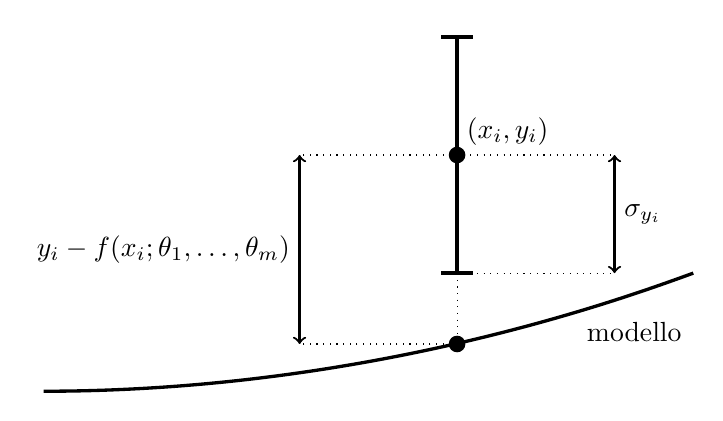
\begin{tikzpicture}
  \node at (0, 0) {};
  \pgfmathsetmacro{\x}{3.}
  \pgfmathsetmacro{\dx}{0.2}
  \pgfmathsetmacro{\qx}{2.0}
  \pgfmathsetmacro{\dy}{1.5}
  \draw[very thick] (\x, 0) -- (\x, -2*\dy);
  \draw[very thick] (\x-\dx, 0) -- (\x+\dx, 0);
  \draw[very thick] (\x-\dx, -2*\dy) -- (\x+\dx, -2*\dy);
  \fill (\x, -\dy) circle [radius=3pt];
  \node[anchor=south west] at (\x, -\dy) {$(x_i, y_i)$};
  \draw[style=dotted] (\x, -\dy) -- (\x + \qx, -\dy);
  \draw[style=dotted] (\x, -2*\dy) -- (\x + \qx, -2*\dy);
  \draw[thick,{<[scale=1.5]}-{>[scale=1.5]}]
  (\x + \qx, -\dy) -- (\x + \qx, -2*\dy);
  \node[anchor=west] at (\x + \qx, -1.5*\dy) {$\sigma_{y_i}$};
  \draw[very thick] (-0.75*\x, -3*\dy) parabola (2*\x,-2*\dy);
  \fill (\x, -2.6*\dy) circle [radius=3pt];
  \draw[style=dotted] (\x, -2*\dy) -- (\x, -2.6*\dy);
  \draw[style=dotted] (\x, -\dy) -- (\x - \qx, -\dy);
  \draw[style=dotted] (\x, -2.6*\dy) -- (\x - \qx, -2.6*\dy);
  \draw[thick,{<[scale=1.5]}-{>[scale=1.5]}]
  (\x - \qx, -\dy) -- (\x - \qx, -2.6*\dy);
  \node[anchor=east] at (\x - \qx, -1.8*\dy)
       {$y_i - f(x_i; \theta_1,\ldots,\theta_m)$};
  \node at (1.75*\x, -2.5*\dy) {modello};
\end{tikzpicture}
}{
    \caption{Significato geometrico dell'$i$-esimo termine della
      somma~\eqref{eq:somma_chiquadro_fit}: il quadrato della distanza
      tra dati e modello (per un insieme di valori dei parametri) misurate in
      barre d'errore.}
    \label{fig:termine_chi2}
  }
\end{figure}

Cominciamo dunque con il costruire la somma, che per motivi che saranno chiari
tra un attimo chiameremo \emph{chi quadro}
\begin{align}\label{eq:somma_chiquadro_fit}
  \chisquare{\theta_1,\ldots,\theta_m} = \sum_{i = 1}^{n}\left(
  \frac{y_i - f(x_i; \theta_1,\ldots,\theta_m)}{\sigma_{y_i}}
  \right)^2.
\end{align}
A questo livello il $\chisq$ non è altro che la \emph{somma dei quadrati
  delle differenze tra dati e modello, misurate in unità di barre d'errore}.
(Non sarete sorpresi del fatto che abbiamo elevato al quadrato le distanze---al
solito è per evitare che fluttuazioni positive e fluttuazioni negative si
cancellino a vicenda.) \`E chiaro allora che questa quantità misura, in un
qualche senso, la distanza complessiva tra una serie di dati ed un modello, in
funzione del valore dei parametri da cui il modello dipende: più piccolo è
il $\chisq$, migliore l'accordo tra dati e modello---e viceversa.

Ora che abbiamo una misura oggettiva dell'accordo tra dati e modello, possiamo
trovare la funzione di \bestfit\ semplicemente minimizzando il nostro
$\chisq$ rispetto agli $m$ parametri del modello:
\begin{align}\label{eq:minimizzazione_chi_quadro}
  \begin{cases}
    \pd{\chisq}{\theta_1}{\hat{\theta}_1,\ldots,\hat{\theta}_m} = 0\\
    \hspace*{30pt}\vdots \\
    \pd{\chisq}{\theta_m}{\hat{\theta}_1,\ldots,\hat{\theta}_m} = 0.\\
   \end{cases}
\end{align}
La~\eqref{eq:minimizzazione_chi_quadro} fornisce un insieme di $m$ equazioni
che, almeno in linea di principio, ci permettono di ricavare gli $m$ valori
di \bestfit\ $\hat{\theta}_1,\ldots,\hat{\theta}_m$ per i parametri.


\subsection{Fit dei minimi quadrati nel caso costante: la media pesata}
\label{sec:media_pesata}

L'esempio più semplice di fit ad un parametro (che chiameremo, per fissare
le idee, $q$) è quello con una funzione costante---cioè indipendente dalla
variabile $x$:
\begin{align*}
  f(x; q) = q \quad \text{(costante)}.
\end{align*}
Illustreremo questo primo caso pedissequamente in ogni passaggio. Il $\chisq$
si scrive come
\begin{align*}
  \chisquare{q} = \sum_{i = 1}^{n}\left(\frac{y_i - q}{\sigma_{y_i}}\right)^2.
\end{align*}
(Notiamo esplicitamente che in questo caso le nostre $n$ misure sperimentali non
saranno coppie ordinate $(x_i$, $y_i$) ma singoli valori $y_i$, poiché nel
modello la variabile indipendente non gioca alcun ruolo.) La condizione di
minimo si scrive ponendo uguale a zero la derivata totale del $\chisq$ rispetto
all'unico parametro
\begin{align}\label{eq:min_chisq_const}
  \td{\chisq}{q}{\hat{q}} =
  -2 \sum_{i = 1}^{n} \left(\frac{y_i - \hat{q}}{\sigma^2_{y_i}}\right) = 0.
\end{align}
Si tratta di un'equazione lineare in $\hat{q}$ che si risolve banalmente, con
poche manipolazioni algebriche, nella forma
\begin{align}\label{eq:media_pesata}
  \hat{q} = \frac{\sum_{i = 1}^{n}\frac{y_i}{\sigma^2_{y_i}}}%
      {\sum_{i = 1}^{n}\frac{1}{\sigma^2_{y_i}}}.
\end{align}
L'espressione~\eqref{eq:media_pesata} si chiama \emph{media pesata} delle $y_i$
e costituisce la procedura statisticamente corretta con cui si combinano misure
indipendenti della stessa quantità---ad esempio risultati di esperimenti
diversi che misurano la stessa grandezza. Il motivo del nome sta nel fatto che
se introduciamo le quantità (che chiameremo \emph{pesi})
\begin{align*}
  w_i = \frac{1}{\sigma^2_{y_i}},
\end{align*}
allora la~\eqref{eq:media_pesata} può essere riscritta nella forma
equivalente, ma più compatta
\begin{align}\label{eq:media_pesata_2}
  \hat{q} = \frac{\sum_{i = 1}^{n} w_iy_i}{\sum_{i = 1}^{n}w_i},
\end{align}
in cui la struttura della media pesata è più facilmente riconoscibile.
Impariamo, come corollario, che i pesi statisticamente corretti da assegnare
alle misure sono dunque gli inversi dei quadrati delle rispettive
incertezze---che, almeno a livello qualitativo, ha senso in quanto le misure
con le incertezze più grandi debbono contare meno nella media.

A questo punto ci rimane da stimare l'incertezza da associare alla nostra stima
$\hat{q}$ di $q$. Formalmente dobbiamo, cioè, calcolare la varianza di
$\hat{q}$
\begin{align}\label{eq:media_pesata_err}
  \sigma^2_q & = \var{\frac{\sum_{i = 1}^{n} w_iy_i}{\sum_{i = 1}^{n}w_i}} =
  \frac{\var{\sum_{i = 1}^{n} w_iy_i}}{\left(\sum_{i = 1}^{n}w_i\right)^2} =
  \frac{\sum_{i = 1}^{n} \var{w_iy_i}}{\left(\sum_{i = 1}^{n}w_i\right)^2} =
  \frac{\sum_{i = 1}^{n} w_i^2\var{y_i}}{\left(\sum_{i = 1}^{n}w_i\right)^2} =
  \nonumber\\
  & = \frac{\sum_{i = 1}^{n} w_i}{\left(\sum_{i = 1}^{n}w_i\right)^2} =
  \frac{1}{\sum_{i = 1}^{n} w_i} =
  \frac{1}{\sum_{i = 1}^n \frac{1}{\sigma^2_i}}.
\end{align}
Il calcolo non è esattamente banale, ma la cosa fondamentale da ricordare
è che, in questo contesto, le $y_i$ sono le variabili casuali mentre
i $\sigma_{y_i}$, e di conseguenza i $w_i$, sono per ipotesi costanti note a
priori, per cui passano fuori (elevate al quadrato, naturalmente) dall'operatore
varianza. Detto questo motiviamo brevemente (ed in ordine) ciascun singolo
passaggio:
\begin{enumerate}
\item abbiamo sfruttato il fatto che $\var{cx} = c^2 \var{x}$,
  cfr.~\eqref{eq:varianza_cost_molt};
\item la varianza della somma è pari alla somma delle varianze
  poiché le $y_i$ sono indipendenti, cfr.~\eqref{eq:media_varianza_somma_ind};
\item abbiamo sfruttato di nuovo il fatto che $\var{cx} = c^2 \var{x}$,
  cfr.~\eqref{eq:varianza_cost_molt};
\item semplice sostituzione: $\var{y_i} = \sigma^2_{y_i} = \nicefrac{1}{w_i}$.
\end{enumerate}
In altre parole il quadrato dell'incertezza su $\hat{q}$ è l'inverso della
somma degli inversi delle incertezze (al quadrato) sulle misure di partenza.
Non è difficile convincersi che $\sigma_q$ è strettamente minore di ciascun
$\sigma_{y_i}$---come è lecito aspettarsi sulla base del fatto che tutte le
misure, più o meno a seconda dell'incertezza associata, contribuiscono
all'informazione.

\begin{examplebox}
  \begin{example}\label{exp:media_pesata}
    Cinque gruppi sperimentali (che chiameremo A\ldots E) misurano
    indipendentemente l'indice di rifrazione dell'acqua ottenendo i valori:
    $n_A = 1.325 \pm 0.012$,
    $n_B = 1.36 \pm 0.05$,
    $n_C = 1.32 \pm 0.01$,
    $n_D = 1.338 \pm 0.005$,
    $n_E = 1.335 \pm 0.006$.
    Se si vogliono combinare le misure per fornire una stima $\hat{n}$ del
    misurando che includa in modo consistente tutta l'informazione disponibile
    il modo corretto di procedere è quello di eseguire una media pesata
    \begin{align*}
      \hat{n} = 1.3339 \pm 0.0034 \quad \text{oppure} \quad
      \hat{n} = 1.334 \pm 0.003.
    \end{align*}
    Il calcolo è implementato nel frammento~\ref{snip:weighted_average} ed
    il risultato è illustrato graficamente nella
    figura~\ref{fig:media_pesata}.
  \end{example}
\end{examplebox}

\pgffigone{media_pesata}{
  Illustrazione del calcolo della media pesata dei valori dell'indice di
  rifrazione nell'esempio~\ref{exp:media_pesata}. La linea continua rappresenta
  il valore della media pesata in questione e le due linee tratteggiate indicano
  l'incertezza (a $1\sigma$) associata. Notiamo esplicitamente che la larghezza
  della banda di incertezza è più piccola della più piccola tra le
  incertezze di misura (quella del gruppo D).
}

\snip{weighted_average}{%
  Frammento di codice per il calcolo della media pesata delle misure dell'indice
  di rifrazione dell'acqua dell'esempio~\ref{exp:media_pesata}. La funzione
  prende in ingresso le liste dei valori delle misure e degli errori
  associati e restituisce la media pesata e l'incertezza associata. Il
  risultato è illustrato graficamente nella figura~\ref{fig:media_pesata}.
  Notiamo, per completezza, che l'incertezza $\sigma_q$ sulla media pesata
  è più piccola del più piccolo tra gli errori di misura.
}


\subsection{Fit dei minimi quadrati nel caso lineare}
\label{sec:min_chisq_lineare}

Il fit dei minimi quadrati nel caso lineare non è solo un esercizio di
notevole importanza pratica; essendo uno degli esempi più semplici di fit a
più di un parametro permette di discutere alcuni aspetti del problema
generale della stima dei parametri che non emergono nella media pesata.
Il nostro modello è in questo caso
\begin{align*}
  f(x; q, m) = mx + q
\end{align*}
da cui
\begin{align*}
  \chisquare{q, m} =
  \sum_{i = 1}^{n}\left(\frac{y_i - mx_i - q}{\sigma_{y_i}}\right)^2.
\end{align*}
Come anticipato, questa volta abbiamo due condizioni di minimo per ricavare
i valori dei due parametri
\begin{align}\label{eq:min_chisq_lineare}
  \begin{cases}
    \displaystyle
    \pd{\chisq}{q}{\hat{q}, \hat{m}} = - 2\sum_{i = 1}^{n}\left(
    \frac{y_i - \hat{m}x_i - \hat{q}}{\sigma_{y_i}^2}\right) = 0\\
    \displaystyle
    \pd{\chisq}{m}{\hat{q}, \hat{m}} = - 2\sum_{i = 1}^{n}\left(
    \frac{y_i - \hat{m}x_i - \hat{q}}{\sigma_{y_i}^2}\right)x_i = 0
  \end{cases}
\end{align}
Allo scopo di semplificare la notazione per il calcolo esplicito della
soluzione, introduciamo alcune quantità---che dipendono solamente dalle misure
sperimentali e \emph{non} dai valori dei parametri del modello, ed i cui valori
numerici possono essere calcolati banalmente una volta che abbiamo a
disposizione le misure stesse:
\begin{align}
  S_x^0 = \sum_{i = 1}^{n} \frac{1}{\sigma_{y_i}^2} \quad
  S_x^1 = \sum_{i = 1}^{n} \frac{x_i}{\sigma_{y_i}^2} \quad
  S_x^2 = \sum_{i = 1}^{n} \frac{x_i^2}{\sigma_{y_i}^2} \quad
  S_{xy}^0 = \sum_{i = 1}^{n} \frac{y_i}{\sigma_{y_i}^2} \quad
  S_{xy}^1 = \sum_{i = 1}^{n} \frac{x_iy_i}{\sigma_{y_i}^2},
\end{align}
col che possiamo allora riscrivere le condizioni di minimo come
\begin{align*}
  \begin{cases}
    \hat{q}S_x^0 + \hat{m}S_x^1 = S_{xy}^0\\
    \hat{q}S_x^1  + \hat{m}S_x^2 = S_{xy}^1
  \end{cases} \quad \text{ovvero, in forma matriciale} \quad
  \begin{bmatrix}
    S_x^0 & S_x^1\\
    S_x^1 & S_x^2
  \end{bmatrix}
  \begin{bmatrix}
    \hat{q}\\
    \hat{m}
  \end{bmatrix} =
  \begin{bmatrix}
    S_{xy}^0\\
    S_{xy}^1
  \end{bmatrix}.
\end{align*}
L'algebra è tediosa, ma concettualmente il calcolo procede esattamente come
per la media pesata nella sezione precedente per cui forniamo direttamente i
risultati. Detta $D$ la quantità
\begin{align*}
  D = S_x^0S_x^2 - (S_x^1)^2
\end{align*}
(che non è altro che il determinante della matrice $2 \times 2$
corrispondente al nostro sistema lineare) si ha:
\begin{align}\label{eq:fit_mq_lineare}
  \begin{cases}
    \displaystyle \hat{q} = \frac{S_{xy}^0 S_x^2 - S_{xy}^1 S_x^1}{D}\\
    \displaystyle \hat{m} = \frac{S_{xy}^1 S_x^0 - S_{xy}^0 S_x^1}{D}
  \end{cases}
  \quad \text{con errori associati} \quad
  \begin{cases}
    \displaystyle \sigma_q^2 = \frac{S_x^2}{D}\\
    \displaystyle \sigma_m^2 = \frac{S_x^0}{D}.
  \end{cases}
\end{align}
Notiamo esplicitamente che, ai fini del calcolo delle incertezze, le uniche
somme che dipendono dalle nostre variabili casuali $y_i$ sono $S_{xy}^0$ ed
$S_{xy}^1$---le altre tre sono semplici \emph{costanti} e possono essere
trattate come tali nel calcolo delle varianze. Per completezza le
quantità rilevanti sono
\begin{align}
  \var{S_{xy}^0} & = \var{\sum_{i = 1}^{n} \frac{y_i}{\sigma_{y_i}^2}} =
  \sum_{i = 1}^{n} \var{\frac{y_i}{\sigma_{y_i}^2}} =
  \sum_{i = 1}^{n} \frac{\var{y_i}}{\sigma_{y_i}^4} =
  \sum_{i = 1}^{n} \frac{1}{\sigma_{y_i}^2} = S_x^0\\
  \var{S_{xy}^1} & =  \var{\sum_{i = 1}^{n} \frac{x_iy_i}{\sigma_{y_i}^2}} =
  \sum_{i = 1}^{n} \var{\frac{x_iy_i}{\sigma_{y_i}^2}} =
  \sum_{i = 1}^{n} \frac{x^2_i\var{y_i}}{\sigma_{y_i}^4} =
  \sum_{i = 1}^{n} \frac{x^2_i}{\sigma_{y_i}^2} = S_x^2 \\
  \cov{S_{xy}^0}{S_{xy}^1} & =
  \cov{\sum_{i = 1}^{n}\frac{y_i}{\sigma_{y_i}^2}}%
      {\sum_{j = 1}^{n}\frac{x_jy_j}{\sigma_{y_j}^2}} =
  \sum_{i, j = 1}^n \frac{x_j}{\sigma^2_{y_i} \sigma^2_{y_j}}\,\cov{y_i}{y_j} =
  \sum_{i = 1}^{n} \frac{x_i}{\sigma_{y_i}^2} = S_x^1,
\end{align}
(nell'ultima relazione abbiamo utilizzato il fatto che $\cov{y_i}{y_j}$ si
annulla per $i \neq j$ ed è uguale a $\sigma^2_{y_i}$ per $i = j$.
Per completezza calcoliamo esplicitamente l'incertezza su $\hat{q}$, lasciando
quella su $\hat{m}$ per esercizio
\begin{align*}
  \sigma^2_q & = \frac{1}{D^2} \left[
    (S_x^2)^2\var{S_{xy}^0} + (S_x^1)^2\var{S_{xy}^1} -
    2S_x^2S_x^1\cov{S_{xy}^0}{S_{xy}^1}
    \right] =\\
  & = \frac{1}{D^2} \left[
    (S_x^2)^2S_x^0 + (S_x^1)^2S_x^2 -
    2S_x^2(S_x^1)^2
    \right] =
  \frac{1}{D^2} \left[ (S_x^2)^2S_x^0 - (S_x^1)^2S_x^2 \right] =
  \frac{S_x^2}{D^2} \left[ S_x^2S_x^0 - (S_x^1)^2 \right] = \frac{S_x^2}{D}.
\end{align*}
(L'unica cosa da ricordare qui è che
$\var{x_1 - x_2} = \var{x_1} + \var{x_2} - 2\cov{x_1}{x_2}$.)
Il frammento di codice~\ref{snip:linear_least_squares} mostra una
implementazione, elementare ma funzionante, dell'algoritmo.

\snip{linear_least_squares}{%
  Esempio di implementazione (funzionante) di un fit dei
  minimi quadrati con un modello lineare. Per chiarezza, i nomi delle variabili
  utilizzate ricalcano da vicino quelli usati nel testo.
}


\subsection{La covarianza tra i parametri nel fit lineare}

A questo punto possiamo chiederci se le quantità $\hat{q}$ e $\hat{m}$ che
abbiamo appena calcolato siano \emph{indipendenti} o meno---e la risposta è
no: anche se le misure $y_i$ da cui partiamo sono, per ipotesi, indipendenti
l'intercetta ed il coefficiente angolare di \bestfit\ sono (negativamente)
correlati. (Non stupirà il fatto che questa non è una peculiarità del
fit dei minimi quadrati lineare ma è una proprietà che vale in generale, a
meno che non si utilizzino tecniche specifiche per evitare la correlazione tra
i parametri di \bestfit.)

In effetti abbiamo già in mano tutti gli ingredienti che ci servono per
calcolare la covarianza cercata, ovverosia
\begin{align}
  \cov{\hat{q}}{\hat{m}} & =
  \cov{\frac{S_{xy}^0 S_x^2 - S_{xy}^1 S_x^1}{D}}%
      {\frac{S_{xy}^1 S_x^0 - S_{xy}^0 S_x^1}{D}} =
      \frac{1}{D^2} \left[
        S_x^0S_x^2\cov{S_{xy}^0}{S_{xy}^1} + \right.\nonumber\\
       & \left. - S_x^1S_x^2\cov{S_{xy}^0}{S_{xy}^0} -
        S_x^0S_x^1\cov{S_{xy}^1}{S_{xy}^1} +
        (S_x^1)^2 \cov{S_{xy}^1}{S_{xy}^0}\right] = \nonumber\\
      & = \frac{1}{D^2} \left[
        S_x^0S_x^1S_x^2 - S_x^0S_x^1S_x^2 - S_x^0S_x^1S_x^2 + (S_x^1)^3
        \right]
      = -\frac{S_x^1\left(S_x^0S_x^2 - (S_x^1)^2 \right)}{D^2} =
      -\frac{S_x^1}{D}.
\end{align}
Ne segue banalmente che le matrici di covarianza e di correlazione tra i
parametri del fit si scrivono come
\begin{align}
  \Sigma = \frac{1}{D}
  \begin{bmatrix}
    S_x^2 & -S_x^1\\
    -S_x^1 & S_x^0
  \end{bmatrix}
  \quad \text{e} \quad
  R =
  \begin{bmatrix}
    1 & -\frac{S_x^1}{\sqrt{S_x^0S_x^2}}\\
    -\frac{S_x^1}{\sqrt{S_x^0S_x^2}} & 1
  \end{bmatrix}
\end{align}

Che la correlazione tra intercetta e coefficiente angolare in un fit sia
diversa da zero (e di segno negativo) non dovrebbe stupire---lo abbiamo già
visto implicitamente parlando della propagazione dell'errore massimo ed è
illustrato nuovamente in figura~\ref{fig:correlazione_inter_coeff}. Il livello
di correlazione tra i parametri aumenta all'aumentare del braccio di leva del
fit e nel limite in cui la dispersione tra i valori $x_i$ è molto più
piccola (in modulo) dei valori numerici degli $x_i$ stessi---cioè quando nella
variabile indipendente i punti sono molto più distanti dall'origine di quanto
non lo siano tra loro stessi---si ha la situazione interessante:
\begin{align}
  x_i \approx \tilde{x} \quad i=1 \ldots n
  \quad \text{da cui} \quad
  S_x^1 \approx \tilde{x} S_x^0, \quad
  S_x^2 \approx \tilde{x}^2 S_x^0
  \quad \text{e infine} \quad
  \corr{\hat{q}}{\hat{m}} = -\frac{S_x^1}{\sqrt{S_x^0S_x^2}} \rightarrow -1.
\end{align}

\pgffigone{correlazione_inter_coeff}{
  Illustrazione grafica della correlazione negativa tra intercetta e
  coefficiente angolare in un fit dei minimi quadrati con un modello lineare.
  La linea continua rappresenta la retta di \bestfit. Le linee
  tratteggiate $r_1$ ed $r_2$ mostrano che se incrementiamo (diminuiamo) il
  valore del coefficiente angolare, per far sì che la retta corrispondente
  continui ad essere un fit accettabile, siamo costretti a diminuire
  (incrementare) il valore dell'intercetta. La barra verticale al
  centro rappresenta l'incertezza (chiaramente assurda) sul valore del modello
  nel punto $x = 5.5$ ottenuta propagando gli errori senza considerare la
  correlazione tra $\hat{q}$ ed $\hat{m}$.
}

Dal punto di vista pratico la cosa è rilevante. Se vogliamo semplicemente
riportare gli errori sui parametri le~\eqref{eq:fit_mq_lineare} sono
sufficienti, ma se vogliamo propagare l'errore su una funzione dei
parametri (ad esempio sull'interpolazione o l'estrapolazione della retta di
\bestfit), allora il fatto che gli elementi fuori dalla diagonale della
matrice di covarianza siano non nulli ci dice che
la~\eqref{eq:propagazione_errore_stat_ind} non vale e siamo costretti ad
utilizzare la~\eqref{eq:propagazione_errore_stat}, come illustrato
nell'esempio~\ref{exp:propagazione_errori_corr}.

\begin{examplebox}
  \begin{example}\label{exp:propagazione_errori_corr}
    Con riferimento al fit lineare in figura~\ref{fig:correlazione_inter_coeff}
    (che include i valori numerici dei parametri e delle incertezze associate)
    supponiamo di voler utilizzare il nostro modello di \bestfit\ per
    stimare l'incertezza di misura associata al valore della variabile
    indipendente $f(x_0)$ in $x_0 = 5.5$. Se propagassimo banalmente gli errori
    come se $\hat{q}$ ed $\hat{m}$ fossero scorrelate avremmo
    \begin{align}
      \sigma^2_f = x_0^2 \sigma_m^2 + \sigma_q^2 \quad \text{ovvero} \quad
      \sigma_f = 0.90
    \end{align}
    che è chiaramente assurdo, come illustrato dalla barra di errore grigia
    in corrispondenza di $x_0$ nella figura~\ref{fig:correlazione_inter_coeff}.
    Il problema è che in questo caso il coefficiente di correlazione tra i
    parametri è prossimo a~$-1$ ed il risultato corretto è
    \begin{align}
      \sigma^2_f = x_0^2 \sigma_m^2 + \sigma_q^2 -
      2x_0\corr{\hat{q}}{\hat{m}}\sigma_q\sigma_m
      \quad \text{ovvero} \quad
      \sigma_f = 0.030
    \end{align}
    che è molto più ragionevole. La differenza tra i due numeri è un
    fattore $20$---non stiamo parlando di una cosa da poco.
  \end{example}
\end{examplebox}


\subsection{Fit dei minimi quadrati con un polinomio di grado arbitrario}

\danger La discussione che abbiamo fatto nelle due sezioni precedenti può
essere generalizzata senza enormi difficoltà (anche se i calcoli tendono a
diventare complicati piuttosto rapidamente) al caso praticamente rilevante del
fit dei minimi quadrati con un polinomio di grado $k$ arbitrario---cioè
del modello
\begin{align}
  f(x; a_0, a_1 \ldots a_k) = a_0 + a_1 x + \cdots + a_k x^k.
\end{align}
L'espressione per il $\chisq$ da minimizzare si scrive in questo caso come
\begin{align*}
  \chisq(a_0, a_1 \ldots a_k) = \sum_{i = 1}^n
  \left( \frac{y_i - (a_0 + a_1 x_i + \cdots + a_k x_i^k)}{\sigma_{y_i}} \right)^2
\end{align*}
e la sua derivata rispetto al generico parametro $a_l$ è banalmente
\begin{align*}
  \td{\chisq}{a_l}{a_0, a_1 \ldots a_k} = -2 \sum_{i = 1}^n
  \left( \frac{y_i - (a_0 + a_1 x_i + \cdots + a_k x_i^k)}{\sigma^2_{y_i}} \right)
  x_i^l.
\end{align*}
Le $k + 1$ condizioni di minimo~\eqref{eq:minimizzazione_chi_quadro} portano
ad un sistema di $k + 1$ equazioni lineari nei parametri
\begin{align}
  \begin{cases}
    \hat{a}_0 \sum_{i = 1}^n \frac{1}{\sigma^2_{y_i}} +
    \hat{a}_1 \sum_{i = 1}^n \frac{x_i}{\sigma^2_{y_i}} + \cdots  +
    \hat{a}_k \sum_{i = 1}^n \frac{x_i^k}{\sigma^2_{y_i}} =
    \sum_{i = 1}^n \frac{y_i}{\sigma^2_{y_i}} \\[8pt]
    \hat{a}_0 \sum_{i = 1}^n \frac{x_i}{\sigma^2_{y_i}} +
    \hat{a}_1 \sum_{i = 1}^n \frac{x_i^2}{\sigma^2_{y_i}} + \cdots  +
    \hat{a}_k \sum_{i = 1}^n \frac{x_i^{k + 1}}{\sigma^2_{y_i}} =
    \sum_{i = 1}^n \frac{x_i y_i}{\sigma^2_{y_i}} \\
    \hspace*{30pt}\vdots \\
    \hat{a}_0 \sum_{i = 1}^n \frac{x_i^k}{\sigma^2_{y_i}} +
    \hat{a}_1 \sum_{i = 1}^n \frac{x_i^{k + 1}}{\sigma^2_{y_i}} + \cdots  +
    \hat{a}_k \sum_{i = 1}^n \frac{x_i^{2k}}{\sigma^2_{y_i}} =
    \sum_{i = 1}^n \frac{x_i^k y_i}{\sigma^2_{y_i}}
   \end{cases}
\end{align}
Definiamo allora, sul modello di ciò che abbiamo fatto nel caso del fit dei
minimi quadrati lineare, le quantità
\begin{align*}
  S_x^l = \sum_{i = 1}^n \frac{x_i^l}{\sigma^2_{y_i}} \quad \text{e} \quad
  S_{xy}^l = \sum_{i = 1}^n \frac{x_i^l y_i}{\sigma^2_{y_i}},
\end{align*}
che, come prima, dipendono solamente dai dati e non dal modello---in altre
parole, una volta che abbiamo le nostre misure, sono delle semplici somme
il cui valore numerico può essere banalmente calcolato.
Il nostro sistema di equazioni può allora essere riscritto in forma matriciale
come
\begin{align}
  \begin{bmatrix}
    S_x^0 & S_x^1 & \cdots & S_x^k\\
    S_x^1 & S_x^2 & \cdots & S_x^{k+1}\\
    \vdots & \vdots & \ddots & \vdots\\
    S_x^k & S_x^{k+1} & \cdots & S_x^{2k}
  \end{bmatrix}
  \begin{bmatrix}
    \hat{a}_0\\
    \hat{a}_1\\
    \vdots\\
    \hat{a}_k
  \end{bmatrix} =
  \begin{bmatrix}
    S_{xy}^0\\
    S_{xy}^1\\
    \vdots\\
    S_{xy}^k
  \end{bmatrix}
\end{align}
a la soluzione passa attraverso una inversione di matrice
\begin{align}
  \begin{bmatrix}
    \hat{a}_0\\
    \hat{a}_1\\
    \vdots\\
    \hat{a}_k
  \end{bmatrix} =
  \begin{bmatrix}
    S_x^0 & S_x^1 & \cdots & S_x^k\\
    S_x^1 & S_x^2 & \cdots & S_x^{k+1}\\
    \vdots & \vdots & \ddots & \vdots\\
    S_x^k & S_x^{k+1} & \cdots & S_x^{2k}
  \end{bmatrix}^{-1}
  \begin{bmatrix}
    S_{xy}^0\\
    S_{xy}^1\\
    \vdots\\
    S_{xy}^k
  \end{bmatrix}
\end{align}
che può essere eseguita utilizzando i metodi ordinari dell'algebra lineare.
(Al di là della soluzione esplicita, la cosa essenziale da ricordare
è che il fit dei minimi quadrati con un polinomio generico porta ad
un insieme di equazioni lineari nei parametri che possono essere risolte
in forma chiusa.)


\subsection{Fit dei minimi quadrati non pesato}

Quando le incertezze di misura $\sigma_{y_i}$ non dipendono dall'indice $i$
(cioè hanno lo stesso valore $\sigma_y$ per tutti i punti sperimentali)
possono passare fuori dal segno di sommatoria e si può utilizzare
l'espressione
\begin{align*}
  \sum_{i = 1}^n (y_i - f(x_i; \theta_1, \ldots, \theta_m))^2
\end{align*}
come quantità da minimizzare nel fit. Va da sé che i $\sigma_{y_i}$ sono
ancora necessari per stimare le incertezze da associare ai parametri e per
calcolare il $\chisq$ del fit, ma le nostre formule si semplificano
sensibilmente. In questo caso si parla di fit dei minimi quadrati
\emph{non pesato}.

Così, per fissare le idee, i risultati che abbiamo ricavato per la media
pesata nella sezione~\ref{sec:media_pesata} divengono, nel caso non pesato
\begin{align}
  \hat{q} = \frac{1}{n}\sum_{i = 1}^n y_i \quad \text{e} \quad
  \sigma_q = \frac{\sigma_y}{\sqrt{n}},
\end{align}
cioè la miglior stima della nostra costante di fit $q$ è data dalla media
aritmetica delle misure $y_i$ (il che non è sorprendente) e per quanto
riguarda l'incertezza associata non abbiamo fatto altro che riscoprire per una
via diversa la formula~\eqref{eq:stdev_media} per la deviazione standard della
media.


\section{Il test del \texorpdfstring{$\chisq$}{chi2}}
\label{sec:test_chi2}

Ora che abbiamo inquadrato il problema generale di \bestfit, e lo abbiamo
risolto nei casi più semplici, è tempo di tornare alla seconda domanda
con cui abbiamo aperto questo capitolo, ovvero: come si fa a decidere se un
fit è soddisfacente o meno? \`E chiaro che, mentre il processo di
minimizzazione del $\chisq$ ci fornisce i valori ottimali dei parametri, la
risposta a questa altra domanda deve essere in qualche modo contenuta nel
valore numerico del $\chisq$ stesso
\begin{align*}
  \chisquare{\hat{\theta}_1,\ldots,\hat{\theta}_m} = \sum_{i = 1}^{n}\left(
  \frac{y_i - f(x_i; \hat{\theta}_1,\ldots,\hat{\theta}_m)}{\sigma_{y_i}}
  \right)^2
\end{align*}
che il fit restituisce in corrispondenza del minimo---ed in questa sezione
cercheremo di capire come.


\subsection{Il contenuto fisico del \texorpdfstring{$\chisq$}{chi2}:
  quanti gradi di libertà?}

Se assumiamo per un attimo che il nostro modello costituisca una descrizione
accurata della realtà e che le incertezze di misura siano stimate
correttamente, allora ogni singolo termine della somma (almeno nel caso in cui
immaginiamo che esso sia calcolato in corrispondenza dei valori veri
$\overline{\theta}_1 \ldots \overline{\theta}_m$ dei parametri)
\begin{align*}
  \zeta_i = \frac{y_i -
    f(x_i; \overline{\theta}_1,\ldots,\overline{\theta}_m)}{\sigma_{y_i}},
\end{align*}
sarà distribuito per definizione come una variabile Gaussiana. Di più: come
una Gaussiana in forma standard, nel senso che
\begin{align*}
  \expect{\zeta_i} &= \expect{\frac{y_i -
      f(x_i; \overline{\theta}_1,\ldots,\overline{\theta}_m)}{\sigma_{y_i}}} =
  \frac{1}{\sigma_{y_i}}\expect{y_i -
    f(x_i; \overline{\theta}_1 \ldots \overline{\theta}_m)} = 0\\
  \var{\zeta_i} &= \expect{\zeta^2} = \frac{1}{\sigma^2_{y_i}}\expect{\left(y_i -
    f(x_i; \overline{\theta}_1 \ldots \overline{\theta}_m)\right)^2} = 1.
\end{align*}
Ora, dato che nella~\eqref{eq:somma_chiquadro_fit} ogni $\zeta_i$ è elevato
al quadrato, la nostra somma è, formalmente, una somma di $n$ variabili
Gaussiane in forma standard al quadrato, e noi abbiamo calcolato esplicitamente
nella sezione~\ref{sec:pdf_chi2} la sua funzione di distribuzione: una
distribuzione del $\chisq$ ad $n$ gradi di libertà. Sappiamo in particolare
che
\begin{align}
  \expect{\chisq(\overline{\theta}_1 \ldots \overline{\theta}_m)} = n
  \quad \text{e} \quad
  \var{\chisq(\overline{\theta}_1 \ldots \overline{\theta}_m)} = 2n.
\end{align}

Possiamo chiederci se tutto questo valga anche se calcoliamo la nostra somma
in corrispondenza dei valori di \bestfit\ dei parametri anziché nei
valori (che peraltro non conosciamo) veri. Ebbene, sotto ipotesi relativamente
deboli la quantità $\chisq(\hat{\theta}_1 \ldots \hat{\theta}_n)$ è
ancora distribuita come un $\chisq$ (cosa che non dimostreremo), ma il numero
rilevante di gradi di libertà non è, in generale, pari al numero $n$ di
misure. Cerchiamo di capire perché.

Supponiamo di fittare la stessa serie di dati con un modello costante $y = q$
ed un modello lineare $y = mx + q$. Ora, è ovvio che, poiché il modello
lineare contiene al suo interno quello costante come caso particolare, esso è
in grado di generare, tra le altre, tutte le funzioni costanti che il primo
modello è in grado di generare. In altre parole il minimo $\chisq$ restituito
da un fit lineare sarà per definizione più piccolo (o al massimo uguale) a
quello restituito da un fit con una costante. Si tratta di una prima
realizzazione importante: il numero di gradi di libertà del nostro problema
non può dipendere solo dal numero di punti che fittiamo---in qualche modo
deve dipendere anche dal numero di parametri liberi che utilizziamo nel fit.
D'altra parte, se torniamo per un attimo al caso limite del fit con un
polinomio di grado $n - 1$, che per definizione passa per tutti i punti, è
chiaro che in quel caso il $\chisq$ del fit è identicamente nullo ed
il nostro numero di gradi di libertà deve essere $0$.

Cambiamo per un attimo prospettiva. Da un punto di vista dei principi primi,
il numero di gradi di libertà del nostro problema è, per definizione, pari
al numero di termini indipendenti nella somma~\eqref{eq:somma_chiquadro_fit}.
Allora è chiaro che per ogni parametro che fittiamo dai nostri dati
introduciamo un vincolo---cioè una relazione tra i dati stessi---che porta
alla diminuzione di un'unità nel numero di gradi di libertà%
\footnote{Ad essere precisi, questo è tecnicamente vero solo nel caso in cui
  il vincolo sia di tipo lineare, ma si tratta di un dettaglio che è
  rilevante solo raramente, in pratica.}.
(Se avete l'impressione che questo vi ricordi qualcosa che abbiamo già visto,
è buon segno---rileggete con attenzione quello che abbiamo detto a proposito
della stima imparziale della varianza campione nella
sezione~\ref{sec:media_varianza_campione}, perché il parallelo con il fatto
che la sostituzione di $\mu$ con $m$ nel numeratore della formula per la
varianza stessa richiedesse la sostituzione di $n$ con $n-1$ al denominatore è
perfettamente calzante).
In definitiva \emph{il numero di gradi di libertà è pari al numero dei punti
  sperimentali $n$ meno il numero di parametri $m$ che stimiamo dal fit}
\begin{align}\label{eq:ndof_fit_punti}
  \nu = n - m.
\end{align}
Vedremo nella sezione~\ref{sec:test_chi2_distribuzione} che nel caso del test
del $\chisq$ per una distribuzione ci sarà un altro piccolo colpo di scena,
ma per il momento questo ci basta.

\begin{examplebox}
  \begin{example}
    Supponiamo di avere una serie di $n$ misure $y_i$, con relative incertezze,
    e di voler verificare con un test del $\chisq$ l'ipotesi che esse siano
    compatibili con una costante $q$. Se questa costante è nota a priori (ad
    esempio dalla teoria), allora il numero di gradi di libertà del problema
    è $\nu = n$. Se, viceversa, abbiamo stimato $q$ a partire dai dati,
    ad esempio mediante un fit dei minimi quadrati, allora
    la~\eqref{eq:media_pesata} ci permette di calcolare il valore di uno
    qualsiasi degli $y_i$, una volta noti i valori di tutti gli altri (oltre
    ovviamente a $\hat{q}$). A questo punto gli $n$ termini della
    somma~\eqref{eq:somma_chiquadro_fit} non sono più tutti indipendenti
    l'uno dall'altro, ed il numero di gradi di libertà è $\nu = n - 1$.
  \end{example}
\end{examplebox}

In pratica, nel prosieguo, indicheremo semplicemente con $\chisq$ la quantità $\chisquare{\hat{\theta}_1,\ldots,\hat{\theta}_m}$, e ci riferiremo ad essa come
\emph{il $\chisq$ del \fit}, con l'intendimento che
\begin{align*}
  \expect{\chisq} = \nu \quad \text{e} \quad \var{\chisq} = 2\nu.
\end{align*}
Ne approfittiamo per introdurre una quantità che si trova spesso usata in
pratica, ovvero il $\chisq$~\emph{ridotto} o $\chisq$~\emph{per grado di libertà}
\begin{align}
  \chisq_\nu = \frac{\chisq}{\nu},
\end{align}
che, banalmente, gode delle proprietà
\begin{align*}
  \expect{\chisq_\nu} = 1 \quad \text{e} \quad \var{\chisq_\nu} = \frac{2}{\nu}.
\end{align*}
(La prima in particolare è semplice da ricordare: il $\chisq$ ridotto del
fit è in media $1$.)



\subsection{Il test del \texorpdfstring{$\chisq$}{chi2} per una serie di dati}
\label{sec:test_chi2_serie}

Siamo finalmente pronti per cominciare. In figura~\ref{fig:chi2_test_ok} è
mostrato un fit ad una serie di $16$ punti sperimentali con un modello
quadratico $f(x) = lx^2 + mx + q$. Il modello ha $3$ parametri per cui sappiamo
che il numero di gradi di libertà del problema è $\nu = 16 - 3 = 13$.

\pgffigone{chi2_test_ok}{
  Esempio di fit ad una serie di dati con un modello quadratico
  $f(x) = lx^2 + mx + q$. Il modello ha $3$ parametri e la serie $16$ punti
  per cui il numero di gradi di libertà è $\nu = 16 - 3 = 13$.
  Il valore del $\chisq$ restituito dal fit è $8.7$. Per completezza
  i contributi di ciascun punto alla somma~\eqref{eq:somma_chiquadro_fit} sono
  riportati sul grafico accanto ai punti stessi---e si tratta di un esercizio
  che è bene abituarsi a fare "ad occhio", perché spesso è utile
  saper stimare approssimativamente il $\chisq$ di un fit senza un calcolatore
  a disposizione.
}

Se osserviamo attentamente la figura, non vi è niente che ci possa indurre a
pensare che questo sia un cattivo fit: i punti sembrano oscillare attorno al
modello di \bestfit\ con differenze dell'ordine delle barre d'errore;
$7$~punti stanno sotto al modello e $9$ sopra, dove in media ce ne aspetteremmo
$8$ e $8$, e non si notano regioni in cui il modello sovrastima o sottostima
sistematicamente i dati; vi sono esattamente $3$ punti che distano
più di una barra d'errore dal modello, quando in media ce ne aspettiamo il
$32\%$ (ovverosia $1$ meno il $68\%$), cioè circa $5$. Insomma, niente che
non vada. Ma cosa ci dice in questo caso il valore del $\chisq$ restituito dal
fit---che, come indicato in figura, è $8.7$?

Ricordiamo ancora una volta le regole del gioco: stiamo dicendo che se noi
eseguissimo molte volte lo stesso esperimento in condizioni di ripetitività,
i punti sperimentali sarebbero diversi ogni volta, così come i valori di
\bestfit\ dei parametri del modello ed il valore del $\chisq$ riportato
dal fit stesso. Se però (i) il modello è appropriato per il sistema fisico
che stiamo studiando e (ii) le incertezze di misura sono stimate in modo
statisticamente corretto (e sono Gaussiane), allora il $\chisq$ del fit
è una variabile casuale distribuita come un chi quadro (appunto) con il numero
appropriato di gradi di libertà.

E nel nostro caso specifico? Beh, $\nu = 13$, per cui ci aspettiamo che il
$\chisq$ valga in media $\mu = \nu = 13$, con una deviazione standard di
$\sigma = \sqrt{2\nu} \approx 5.10$. Il valore $8.7$ che abbiamo ottenuto è
entro una deviazione standard dalla media, per cui non abbiamo niente di cui
preoccuparci. Possiamo fare di più: possiamo consultare le tavole in
appendice~\ref{sec:tavola_chisq1}, da cui leggiamo che per un $\chisq$ a
$13$ gradi di libertà
\begin{align*}
  \prob{\chisq_{13} \leq 8.7} \approx 20\%
\end{align*}
(abbiamo interpolato più o meno ad occhio tra i valori $7.04$ e $9.30$ che si
trovano in tabella): se ripetessimo molte volte l'esperimento nel $20\%$ dei
casi otterremo un $\chisq$ minore e nell'$80\%$ dei casi un $\chisq$ maggiore,
ma il punto è che nessuno di questi due numeri è \emph{troppo vicino} a $0$,
per cui possiamo concludere che il nostro fit è un buon fit. Ora, questa è
materia scivolosa che si presta facilmente a fraintendimenti per cui è bene
chiarire le cose via via che si presentano.
\emph{Dire che un fit è un buon fit non equivale a dire che il modello è
  corretto.} (Per inciso, non si può mai dire che un modello è
corretto perché in futuro misure più precise potrebbero dimostrare che non
lo è. Può sembrare triste, ma l'unica cosa che si può veramente concludere
in Fisica è che un modello è sbagliato.)
Invece: \emph{Dire che un fit è un buon fit equivale a dire che non abbiamo
ragioni per rigettare il nostro modello.} Teniamolo ben in mente, perché non
si tratta di semplice semantica, e ne parleremo più diffusamente nella
sezione~\ref{sec:pvalue}.

Abbiamo sviscerato in modo esaustivo il caso (relativamente semplice) in cui
tutto va bene, ed è ora giunto il momento di esaminare in dettaglio l'ampia
zoologia dei \emph{fit cattivi}. Iniziamo con i due casi in cui il $\chisq$ è
troppo alto mostrati
in figura~\ref{fig:chi2_test_modello_cattivo_chi2_test_errori_sottostimati},
che rappresentano un fit lineare degli stessi dati di
figura~\ref{fig:chi2_test_ok} ed un fit quadratico ove però le barre d'errore
sono state deliberatamente rimpicciolite.

\pgffigtwo{chi2_test_modello_cattivo}{chi2_test_errori_sottostimati}{
  Esempi di fit lineare (a sinistra) e quadratico (a destra) degli stessi punti
  sperimentali di figura~\ref{fig:chi2_test_ok}---nel secondo caso le barre
  d'errore sono state volutamente ridotte. In entrambi i casi il valore del
  $\chisq$ è troppo alto, ed indica un cattivo fit. (Notiamo
  esplicitamente che il fit lineare ha $2$ parametri anziché $3$, per cui il
  numero di gradi di libertà passa da $13$ a $14$.)
}

Per prima cosa: con $14$ gradi di libertà ci aspettiamo un $\chisq$ di
$14$ con una deviazione standard di $\sqrt{28} \approx 5.29$, mentre con $13$
gradi di libertà, come già sappiamo, ci aspettiamo un $\chisq$ di $13$
con una deviazione standard di $\sqrt{26} \approx 5.10$. In entrambi i casi
mostrati in
figura~\ref{fig:chi2_test_modello_cattivo_chi2_test_errori_sottostimati} il
valore del $\chisq$ restituito dal fit dista qualcosa dell'ordine di $7$--$8$
deviazioni standard dalla media---cioè è troppo grande. (Ora, visto che
abbiamo detto che il $\chisq$ è una sorta di misura della distanza
complessiva del modello dai dati, il fatto che sia troppo grande deve essere
male, non vi pare?) Possiamo di nuovo consultare le tavole in
appendice~\ref{sec:tavola_chisq1}, che in questo caso ci dicono
\begin{align*}
  \prob{\chisq_{14} \leq 51.2} > 99.99\% \quad \text{e} \quad
  \prob{\chisq_{13} \leq 54.2} > 99.99\%.
\end{align*}
Fermiamoci un secondo: stiamo dicendo che se ripetessimo l'esperimento e se (i)
il modello fosse corretto e (ii) gli errori stimati correttamente, allora la
probabilità di ottenere un $\chisq$ minore di quello che abbiamo ottenuto
sarebbe maggiore del $99.99\%$. Cioè che, nelle nostre due ipotesi, otterremo
un $\chisq$ pari o maggiore a quello che abbiamo ottenuto in meno (e
probabilmente molto meno) di un caso su $10000$. A questo punto siamo costretti
a scegliere tra due possibilità: o siamo stati incredibilmente sfortunati,
oppure una delle nostre due assunzioni (o entrambe) non è verificata.
Da Fisici, optiamo per la seconda---ed anticipiamo che la soglia per decidere
in un verso o nell'altro è completamente arbitraria, ma ci torneremo più in
dettaglio nella sezione~\ref{sec:pvalue}.

Allora, se il $\chisq$ è troppo grande si hanno due casi, che sono legati uno
ad uno alle nostre due ipotesi di lavoro: o il numeratore della
somma~\eqref{eq:somma_chiquadro_fit} è troppo grande (cioè il nostro
modello non è adeguato a fittare i dati) oppure il denominatore è troppo
piccolo (cioè gli errori sono sottostimati). La differenza è, anche
visualmente, ovvia nei due grafici in
figura~\ref{fig:chi2_test_modello_cattivo_chi2_test_errori_sottostimati}: in
quello a sinistra si vede chiaramente che i punti sperimentali hanno una certa
concavità che il modello lineare non è in grado di catturare (nella parte
centrale ci sono $8$ punti consecutivi che stanno sotto al modello); in quello
a destra gli errori sono semplicemente troppo piccoli. Nella realtà le due
cose possono presentarsi insieme in modo difficilmente fattorizzabile, ma è
ugualmente importante allenare l'occhio ad identificare questo tipo di
situazioni.

Non abbiamo ancora finito. Ci rimane da trattare il caso in cui il $\chisq$
è troppo piccolo. (Se siete tentati di dire che un $\chisq$ piccolo non è
un problema perché implica che il modello è molto vicino ai dati, non
smettete di leggere perché vi sbagliate---e di grosso).

\pgffigtwo{chi2_test_overfitting}{chi2_test_errori_sovrastimati}{
  Esempi di fit con un polinomio di grado $4$ (a sinistra) e quadratico (a
  destra) degli stessi punti sperimentali in figura~\ref{fig:chi2_test_ok}---nel
  secondo caso le barre d'errore sono state volutamente allargate. In entrambi
  i casi il valore del $\chisq$ è troppo basso, ed indica un cattivo
  fit.
}

La figura~\ref{fig:chi2_test_overfitting_chi2_test_errori_sovrastimati} mostra
un esempio di fit dei dati in figura~\ref{fig:chi2_test_ok} con un
polinomio di grado $4$ ed un fit quadratico in cui gli errori sono stati
volutamente aumentati. Dalle tabelle in appendice~\ref{sec:tavola_chisq1}
leggiamo
\begin{align*}
  \prob{\chisq_{11} \leq 4.1} \approx 2\% \quad \text{e} \quad
  \prob{\chisq_{13} \leq 1.4} < 0.5\%.
\end{align*}
Cioè: se ripetessimo l'esperimento e se (i) il modello fosse corretto e (ii)
gli errori stimati correttamente, la probabilità di ottenere un $\chisq$ pari
a quello ottenuto o più piccolo sarebbe molto piccola---otterremmo quasi
sempre un $\chisq$ più grande. Da Fisici, allora, dobbiamo accettare di nuovo
che evidentemente una delle nostre ipotesi di lavoro (o entrambe) non è
verificata. Il ragionamento procede esattamente come prima, e una delle
possibilità è che abbiamo banalmente sovrastimato gli errori, come mostrato
nel pannello di destra della
figura~\ref{fig:chi2_test_overfitting_chi2_test_errori_sovrastimati}.
Ma ce n'è un'altra, e cioè che il nostro modello sia troppo
\emph{flessibile}; quando ciò accade, esso tende ad adattarsi alle
fluttuazioni statistiche dei dati, ed il fit diviene artificialmente troppo
buono, con un $\chisq$ corrispondentemente troppo piccolo---ma se ripetessimo
l'esperimento su campione di dati diverso, il nostro modello di \bestfit\
sarebbe con ogni probabilità pessimo. Per completezza, questo fenomeno è
noto come \foreign{over-fitting}, e l'esempio estremo è di nuovo l'interpolazione
con un polinomio di grado $n - 1$ che abbiamo tirato in ballo più volte
dall'inizio del capitolo.


\subsection{Il grafico dei residui}
\label{sec:grafico_residui}

Una rappresentazione utile del fit che si trova spesso usata in pratica
è il cosiddetto \emph{grafico dei residui}, in cui si mostra, in funzione
della variabile indipendente, la differenza tra i punti misurati ed il modello,
calcolato in corrispondenza dei valori di \bestfit\ dei parametri (e
dunque senza incertezze associate):
\begin{align*}
  r_i = y_i - f(x_i; \hat{\theta}_1, \ldots, \hat{\theta}_m)
  \quad \text{e} \quad
  \sigma_{r_i} = \sigma_{y_i}.
\end{align*}
Il modello di \bestfit\ coincide dunque con l'asse $y = 0$ e le
differenze tra dati e modello sono visualizzate in modo più efficace che non
in un grafico semplice in cui dati e modello sono banalmente sovrapposti.
Spesso il grafico dei residui è combinato con il grafico ordinario nella
forma di due pannelli sovrapposti, come mostrato in
figura~\ref{fig:chi2_test_residui}.

\pgffigone{chi2_test_residui}{
  Esempio di grafico dei residui corrispondente al grafico di sinistra della
  figura~\ref{fig:chi2_test_modello_cattivo_chi2_test_errori_sottostimati}
  Il pannello inferiore (dei residui, appunto) mostra direttamente le
  deviazioni dei punti misurati rispetto al modello, e rende più facile
  valutare qualitativamente la bontà del fit. Notiamo esplicitamente che,
  poiché il modello è calcolato in un punto fissato, i valori numerici delle
  incertezze associate ai residui sono identiche alle incertezze di misura
  di partenza $\sigma_{y_i}$.
}


\subsection{Fit dei minimi quadrati e test del \texorpdfstring{$\chisq$}{chi2}
  per una distribuzione}
\label{sec:test_chi2_distribuzione}

Supponiamo adesso di voler fare un fit dei minimi quadrati o un test del
$\chisq$ nel caso di una distribuzione---ad esempio, potremmo lanciare un dado
a sei facce per $100$ volte e vedere se l'ipotesi che il dado sia equo può
essere rigettata. Oppure potremmo voler confrontare in senso statistico un
istogramma con una distribuzione di variabile continua (e.g., una Gaussiana).
\`E chiaro che questo problema è legato a quanto abbiamo detto fino a questo
momento nella prima parte del capitolo. Ma come possiamo costruire una grandezza
che sia l'equivalente della~\eqref{eq:somma_chiquadro_fit} in questo nuovo
contesto?

La differenza fondamentale è che qui non abbiamo a che vedere con misure
sperimentali, ma con \emph{conteggi}. Cominciamo con l'indicare con $o_i$ le
occorrenze osservate in corrispondenza dell'$i$-esimo valore della nostra
variabile discreta o dell'$i$-esimo canale del nostro istogramma. Il modello,
d'altra parte, ci permetterà in generale (eventualmente in funzione dei
suoi parametri) di calcolare le occorrenze attese $e_i$ nella forma
\begin{align}
  e_i(\theta_1, \ldots, \theta_m) =
  \begin{cases}
    \displaystyle N \prob{x_i; \theta_1, \ldots, \theta_m} &
    \text{per una distribuzione di variabile discreta}\\
    \displaystyle N \int_{x_i}^{x_{i+1}} p(x; \theta_1, \ldots, \theta_m)dx
    & \text{per un istogramma}
  \end{cases}
\end{align}
dove l'ultimo integrale è inteso tra gli estremi dell'$i$-esimo canale
dell'istogramma ed $N$ è il numero totale $N = \sum_i o_i$ di occorrenze
osservate.

\begin{examplebox}
  \begin{example}
    Nel caso dei nostri $100$ lanci di un dado le occorrenze osservate $o_i$
    sono banalmente il numero di volte in cui ogni faccia è uscita.
    (Notiamo che si ha il vincolo $\sum_{i=1}^6 o_i = 100$.) Se ipotizziamo che
    il dado sia equo, il nostro modello prevede che le occorrenze attese siano
    identiche tra loro e pari a $e_i = \nicefrac{100}{6}$.
  \end{example}
\end{examplebox}

Con questi ingredienti possiamo scrivere quella che anticipiamo essere la
risposta corretta alla nostra domanda iniziale, ovvero:
\begin{align}\label{eq:somma_chiquadro_dist}
  \chisq = \sum_{i = 1}^n
  \frac{(o_i - e_i(\theta_1, \ldots, \theta_m))^2}
       {e_i(\theta_1, \ldots, \theta_m)}
       \quad \text{o più semplicemente} \quad
       \chisq = \sum_{i = 1}^n\frac{(o_i - e_i)^2}{e_i}.
\end{align}
Fermiamoci per un secondo. Non vi è dubbio che
la~\eqref{eq:somma_chiquadro_dist} ricordi, almeno superficialmente,
la~\eqref{eq:somma_chiquadro_fit}.
Il numeratore $(o_i - e_i(\theta_1, \ldots, \theta_m))^2$ è banalmente la
riscrittura di $(y_i - f(x_i; \theta_1, \ldots, \theta_m))^2$,
a patto di identificare $o_i \rightarrow y_i$---ciò che abbiamo misurato---ed
$e_i(\theta_1,\ldots,\theta_m) \rightarrow f(x_i;\theta_1,\ldots,\theta_m)$---%
ovvero ciò che prevede il modello.
Al denominatore abbiamo bisogno di una stima dell'errore di misura, che in
questo caso coinciderà con la deviazione standard della distribuzione dei
conteggi attesi $e_i$. Ma noi siamo abituati (lo abbiamo visto per le
distribuzioni binomiale e Poissoniana) al fatto che gli errori sui conteggi
scalano con la radice dei conteggi stessi $\sigma_{e_i} \approx \sqrt{e_i}$
ovvero $\sigma^2_{e_i} \approx e_i$. La~\eqref{eq:somma_chiquadro_dist} è
dunque perfettamente ragionevole, sulla base di tutto quello che abbiamo
imparato fino a questo momento.

C'è ancora un punto, sottile ma estremamente importante, da discutere.
Nei casi in cui il numero totale $N$ di eventi (o conteggi) è
\emph{fissato}---ad esempio perché abbiamo deciso a priori di lanciare la
nostra moneta o il nostro dado $100$~volte---gli $n$ elementi della
somma~\eqref{eq:somma_chiquadro_dist} non sono più tutti indipendenti tra di
loro, perché non sono più indipendenti tra di loro le grandezze $o_i$.
Se conosciamo il valore di $n-1$ occorrenze possiamo calcolare banalmente la
rimanente attraverso
\begin{align*}
  o_k = N - \sum_{i \neq k} o_i, \quad \text{ad esempio} \quad
  o_n = N - \sum_{i = 0}^{n - 1} o_i.
\end{align*}
Ma si tratta di una cosa cui siamo ormai avvezzi: abbiamo un vincolo ulteriore
che riduce di una unità il numero di gradi di libertà, per cui nel contesto
del test del $\chisq$ per una distribuzione la~\eqref{eq:ndof_fit_punti} diviene
\begin{align}\label{eq:ndof_fit_dist}
  \nu = n - m - 1.
\end{align}
Ovvero: quando si ha a che fare con una variabile casuale discreta o un
istogramma ed il numero totale di conteggi è fissato, \emph{il numero di
  gradi di libertà è pari al numero dei dati sperimentali $n$ meno il
  numero di parametri $m$ che stimiamo dal fit meno $1$}.


\subsection{Poissoniana o binomiale? Un semplice esempio}

\`E arrivato il momento di osservare più da vicino
la~\eqref{eq:somma_chiquadro_dist}. Molti di voi saranno saltati sulla sedia
gridando: certo! La statistica dei conteggi è Poissoniana, e dato un numero
di conteggi medio $e_i$ la deviazione standard corrispondente è $\sqrt{e_i}$,
per cui il denominatore della~\eqref{eq:somma_chiquadro_dist} rappresenta
esattamente l'equivalente del quadrato dell'errore di misura. Di più:
poiché se gli $e_i$ sono abbastanza grandi la distribuzione di Poisson può
essere approssimata con una Gaussiana, la~\eqref{eq:somma_chiquadro_dist} tende
in questo limite alla somma di $n$ variabili Gaussiane in forma standard
indipendenti, per cui ha proprio il significato di un $\chisq$.

Tutto questo è vero quando il numero totale di conteggi non è fissato, ma
nel caso tipico in cui decidiamo a priori quante volte vogliamo ripetere un
esperimento (e.g., i nostri soliti $100$ lanci di un dado) le cose sono più
complicate---anche se la~\eqref{eq:somma_chiquadro_dist}, come vedremo tra un
attimo, costituisce ancora la risposta corretta. In questo caso, se consideriamo
l'$i$-esimo valore della variabile casuale in questione (o l'$i$-esimo canale
dell'istogramma) \emph{contro tutti gli altri}, non è difficile rendersi conto
che il problema è in realtà binomiale. Per chiarire le idee con un
esempio, se (con la consueta fantasia) lanciamo un dado a $6$ facce per $100$
volte, il numero di volte $o_2$ in cui esce la faccia $2$ sarà una
variabile casuale distribuita secondo una binomiale
$\binomialpdf[100, \nicefrac{1}{6}]{o_2}$. In generale, detta $p_i = \prob{x_i}$
la probabilità elementare che l'esito del nostro esperimento coincida con il
valore $i$-esimo $x_i$ della variabile casuale in questione o cada nel canale
$i$-esimo del nostro istogramma, le occorrenze corrispondenti $o_i$ saranno
distribuite come una binomiale $\binomialpdf[N, p_i]{o_i}$, con
\begin{align}
  \expect{o_i} = N p_i = e_i \quad \text{e} \quad
  \var{o_i} = N p_i(1 - p_i) \neq e_i.
\end{align}
Il problema sta proprio nel fatto che in questo caso la varianza delle
occorrenze attese è diversa dal valore di aspettazione delle occorrenze
stesse, ed uno può legittimamente chiedersi dove sia finito il fattore
$(1 - p_i)$ che, ingenuamente, ci aspetteremmo di vedere al denominatore
della~\eqref{eq:somma_chiquadro_dist}. Lo vediamo in pratica con un esempio
elementare.

Supponiamo dunque di lanciare una moneta $N$ volte e di ottenere un numero di
teste $o_t$ ed un numero di croci $o_c$. A costo di essere pedanti ripetiamo che
la somma $o_t + o_c = N$ è fissata per cui $o_c$ ed $o_t$ non sono
indipendenti---e.g., il numero di croci è fissato dal numero di teste nella
forma di $o_c = N - o_t$. Indichiamo con $p$ la probabilità che l'uscita sia
testa, e fissiamo $p = \nicefrac{1}{2}$ a priori perché vogliamo verificare
l'ipotesi che la moneta sia equa. In queste condizioni il modello, che è
completamente specificato e non ha parametri liberi se non la normalizzazione,
prevede
\begin{align*}
  e_t = N p \quad \text{e} \quad
  e_c = N(1 - p),
\end{align*}
per cui il nostro conteggio del numero di gradi di libertà è
$\nu = n - m - 1 = 2 - 0 - 1 = 1$. Proviamo a mettere tutto insieme e scrivere
la~\eqref{eq:somma_chiquadro_dist} nel nostro caso specifico
\begin{align*}
  \chisq & = \frac{(o_t - e_t)^2}{e_t} + \frac{(o_c - e_c)^2}{e_c} =
  \frac{(o_t - N p)^2}{N p} + \frac{(o_c - N(1 - p))^2}{N(1 - p)} = \\
  & = \frac{(1 - p)(o_t - N p)^2 + p(o_c - N(1 - p))^2}{N p(1 - p)} =
  \frac{(1 - p)(o_t - N p)^2 + p(o_t - N p)^2}{N p(1 - p)} =
  \frac{(o_t - N p)^2}{N p(1 - p)} =\\
  & = \frac{(o_t - e_t)^2}{e_t(1 - p)}.
\end{align*}
(Nel terzultimo passaggio abbiamo eliminato $o_c$ sfruttando la condizione di
normalizzazione.) La nostra semplice manipolazione algebrica ha sortito due
effetti distinti. Il primo è che, una volta scritta in funzione delle sole
variabili indipendenti, la~\eqref{eq:somma_chiquadro_dist} ha un solo termine
(e quindi, come avevamo anticipato) un solo grado di libertà anziché due.
La seconda è che adesso al denominatore riconosciamo la varianza del numero
atteso di teste $e_t$ nell'ipotesi (corretta) che essa sia distribuita come una
binomiale.

Il gioco funziona anche per $n > 2$ e, con un leggero abuso di
termini, potremmo dire che la~\eqref{eq:somma_chiquadro_dist} è corretta
perché \emph{maschera} da somma di $n$ variabili Poissoniane indipendenti---in
una forma elegante e simmetrica---quella che in realtà è la somma di
$n - 1$ variabili binomiali.

Ora, quando i valori medi attesi $e_i$ sono abbastanza grandi%
\footnote{Non esiste un limite netto a cosa significhi \emph{abbastanza grande},
  anche se in alcuni testi si trova $e_i \geq 5$. Se il numero di occorrenze
  per un determinato termine della somma è però inferiore ad $1$ o $2$
  conviene sicuramente aggregare il termine stesso con uno (o più) dei vicini
  prima di calcolare il $\chisq$.}
la distribuzione (binomiale) di ciascun termine della somma tende ad una
Gaussiana in forma standard ed il cerchio si chiude, poiché
la~\eqref{eq:somma_chiquadro_dist} acquista, sia pure solo approssimativamente,
il significato di una variabile $\chisq$ e tutto quello che abbiamo discusso
nella sezione precedente, \emph{mutatis mutandis}, vale anche qui. (Per inciso,
abbiamo discusso il caso di una distribuzione nel contesto del test del
$\chisq$, ma va da sé che il tutto si applica anche alla stima di parametri
mediante fit dei minimi quadrati.)

\begin{examplebox}
  \begin{example}\label{exp:chi2_dado_1}
    Si lancia un dado a sei facce per $100$ volte, ottenendo per le facce
    $1 \ldots 6$ le seguenti occorrenze: $13$, $12$, $14$, $20$, $22$, $19$.
    Possiamo concludere che il dado non è equo?
    \begin{minipage}{0.65\textwidth}
      Si tratta di una semplice applicazione del test del $\chisq$, in cui
      il numero atteso di occorrenze per ciascuna faccia è \nicefrac{100}{6}.
      Possiamo usare la tabella qui di fianco per costruire la
      somma~\eqref{eq:somma_chiquadro_dist}. Abbiamo $n = 6$ punti e, poiché
      il modello è completamente specificato (non abbiamo stimato nessun
      parametro dai dati) il numero di gradi di libertà del problema è
      $\nu = 6 - 0 - 1 = 5$. Il valore del $\chisq$ che abbiamo ottenuto è
      $5.24$, che è abbondantemente entro una deviazione standard dalla media
      attesa per $5$ gradi di libertà, per cui non abbiamo ragione di pensare
      che il dado sia truccato.
    \end{minipage}\hfill\begin{minipage}[c]{0.3\textwidth}
    \begin{tabular}{lll}
        \hline
        $o_i$ & $e_i$ & $\nicefrac{(o_i - e_i)^2}{e_i}$\\
        \hline
        \hline
        $13$ & $16.67$ & $0.808$\\
        $12$ & $16.67$ & $1.308$\\
        $14$ & $16.67$ & $0.428$\\
        $20$ & $16.67$ & $0.665$\\
        $22$ & $16.67$ & $1.704$\\
        $19$ & $16.67$ & $0.326$\\
        \hline
        $100$ & $100$ & $5.24$\\
        \hline
      \end{tabular}
    \end{minipage}
  \end{example}

  \begin{example}\label{exp:chi2_dado_2}
    Si lancia un dado a sei facce per $10000$ volte, ottenendo per le facce
    $1 \ldots 6$ le seguenti occorrenze: $1300$, $1200$, $1400$, $2000$, $2200$,
    $1900$ (si tratta dell'esempio precedente in cui abbiamo moltiplicato tutti
    i numeri per un fattore $100$). Cambiano le conclusioni?
    Anche senza costruire esplicitamente la tabella possiamo notare che in
    questo caso stiamo moltiplicando tutti i numeratori della somma per $100^2$
    ed i denominatori per $100$, per cui l'effetto netto sarà che il $\chisq$
    in questo caso è $100$ volte più grande. Il numero di gradi di
    libertà è ancora $5$ e con un $\chisq$ di $524$ per $5$ gradi di
    libertà possiamo affermare senza ombra di dubbio che il dado è
    truccato.
  \end{example}
\end{examplebox}


\subsection{Il concetto di \emph{\texorpdfstring{$p$}{p}-value}}
\label{sec:pvalue}

Possiamo riassumere sommariamente quanto visto nelle sezioni precedenti dicendo
che, quando facciamo un test del $\chisq$ per un fit con $\nu$ gradi di
libertà, ci aspettiamo il valore numerico del $\chisq$ stesso sia in media
$\nu$, con una deviazione standard di $\sqrt{2\nu}$. Se il risultato è entro
$2$--$3$ deviazioni standard dalla media, non abbiamo ragione di rigettare il
modello. Se il $\chisq$ è troppo grande, questo significa che il modello è
inadeguato oppure gli errori sono sottostimati---o una combinazione delle due
cose. Se il $\chisq$ è troppo piccolo, ciò significa che il modello ha
troppi parametri oppure gli errori sono sovrastimati---o, di nuovo, una
combinazione delle due. Ora, il test del $\chisq$ è il primo esempio di
\emph{verifica delle ipotesi} che incontriamo nel nostro percorso. Fino a
questo momento ci siamo concentrati sulla sua applicazione al problema della
bontà di un fit, ma più in generale, il $\chisq$ è una \emph{statistica}
(o \foreign{test statistics} in inglese) che può essere utilizzato anche quando
non è esplicitamente in gioco un fit.

In effetti gli esempi~\ref{exp:chi2_dado_1} e~\ref{exp:chi2_dado_2} sono
rappresentativi della situazione in cui il modello che utilizziamo per il test
è completamente specificato indipendentemente dalle osservazioni, e noi siamo
semplicemente interessati a verificare la presenza o meno di un effetto fisico
("il dado è truccato?"). Possiamo anche riformulare il problema ribaltando
la logica e chiederci se abbiamo elementi per rigettare l'ipotesi che l'effetto
fisico che cerchiamo \emph{non} sia all'opera ("il dado è equo?"").
Quest'ultima si chiama tipicamente \emph{ipotesi nulla} e si denota con $H_0$,
e nel contesto della verifica delle ipotesi si definisce \pvalue\ la
\emph{probabilità di ottenere un risultato (e.g., un valore di $\chisq$)
  uguale o più estremo di quello che abbiamo ottenuto, assumendo che
  l'ipotesi nulla sia verificata}. Si tratta di una definizione piuttosto
involuta, ma intuitivamente possiamo dire che il \pvalue\ misura il livello
di incompatibilità di un particolare insieme di dati con un modello
statistico---e più è piccolo il \pvalue, più è grande questa
incompatibilità. Un valore troppo piccolo di \pvalue\ può allora essere
interpretato come un'evidenza a sfavore dell'ipotesi nulla---sempre che tutte
le assunzioni che vanno nel calcolo del \pvalue\ stesso siano verificate.

Quello di \pvalue\ è uno dei concetti più controversi nella statistica
moderna~\cite{dagostini_pvalues,asa_pvalues}, tanto che il suo uso è stato
recentemente bandito, non senza che questo destasse scalpore, da una nota
rivista scientifica Statunitense: \foreign{Basic and Applied Social Psychology}.
E il motivo di fondo della controversia è il fatto che la letteratura---sia
quella specialistica che quella divulgativa---è costellata di cattivi esempi
in cui il concetto di \pvalue, usato in modo fondamentalmente scorretto, ha
generato confusione e disinformazione (per non parlare dei casi in cui il
\pvalue\ è stato usato in modo deliberatamente fraudolento per supportare
conclusioni non corroborate dai dati). Questo è dunque un buon momento per
chiarire cosa \emph{non è} il \pvalue.

\begin{itemize}
\item \emph{Il \pvalue\ non è la probabilità che l'ipotesi nulla sia
  corretta}. La differenza può sembrare sottile, ma tornate per un attimo a
  rileggere la nostra definizione iniziale: essa è un'affermazione
  probabilistica a proposito dei dati (in relazione ad una certa ipotesi $H_0$)
  e non a proposito dell'ipotesi. In altre parole, a questo punto dovremmo
  avere gli strumenti per capire al volo che le probabilità condizionate
  $\prob{\text{dati} \cond H_0}$ e $\prob{H_0 \cond \text{dati}}$ non sono la
  stessa cosa. Così come non diremmo mai che la probabilità che un senatore
  sia donna è uguale alla probabilità che una donna sia senatore, allo
  stesso modo non dobbiamo farci ingannare da questo.
\item A maggior ragione \emph{il \pvalue\ non è la probabilità che
  l'ipotesi alternativa ad $H_0$ sia errata}---ovverosia $(1 - \text{\pvalue})$
  non è la probabilità che l'ipotesi alternativa ad $H_0$ sia corretta.
\item \emph{Il \pvalue\ non è la probabilità che quello che abbiamo
  osservato sia semplicemente l'effetto di una fluttuazione statistica}.
  Il calcolo del~\pvalue\ è basato esattamente sull'assunzione che
  la nostra osservazione sia il prodotto del caso (sotto l'ipotesi nulla) per
  cui è chiaro che non può essere utilizzato per stimare la probabilità
  di questa assunzione.
\item \emph{Il \pvalue\ non è la probabilità di rigettare per sbaglio
  l'ipotesi nulla}. Di nuovo: la nostra definizione di \pvalue\ è
  un'affermazione a proposito dei dati, non dell'ipotesi nulla.
\end{itemize}

\begin{examplebox}
  \begin{example}
    Supponiamo di aver lanciato un dado a sei facce per $100000$ volte e di
    aver fatto un test del $\chisq$, come negli esempi~\ref{exp:chi2_dado_1}
    e~\ref{exp:chi2_dado_2}, che ha fornito questa volta un valore di $35.5$.
    La nostra ipotesi nulla $H_0$ è il fatto che il dado sia equo.
    Si tratta di un'ipotesi completamente specificata, che costituisce una
    descrizione completa del nostro problema e ci permette di calcolare le
    occorrenze attese da utilizzare nel test del $\chisq$.
    Il \pvalue\ coincide con la probabilità che un $\chisq$ a $5$ gradi di
    libertà sia maggiore o uguale a $35.5$ e può essere calcolato facilmente
    con un \foreign{computer}
    \begin{align*}
      \text{\pvalue} = \prob{\chisq_5 \geq 35.5} \approx 1.2 \times 10^{-6}.
    \end{align*}
    Ora, quello che in sostanza il \pvalue\ ci dice in questo caso è che
    se il dado fosse equo e noi ripetessimo il nostro esperimento (cioè i
    nostri $100000$ lanci) molte volte, allora otterremmo un $\chisq$ maggiore
    o uguale a quello che abbiamo ottenuto in questo primo tentativo ($35.5$)
    circa una volta su un milione.
    In questo caso il valore basso di \pvalue\ può essere interpretato come
    un'evidenza a sfavore dell'ipotesi nulla---cioè siamo costretti ad
    accettare che il dado non sia equo. Detto questo:
    \begin{itemize}
    \item $1.2 \times 10^{-6}$ non è la probabilità che il dado sia equo;
    \item $(1 - 1.2 \times 10^{-6})$ non è la probabilità che il dado non
      sia equo;
    \item $1.2 \times 10^{-6}$ non è la probabilità di aver osservato una
      fluttuazione statistica;
    \item $1.2 \times 10^{-6}$ non è la probabilità di commettere un errore
      dicendo che il dado non è equo.
    \end{itemize}
  \end{example}

    \begin{example}
    Un test del $\chisq$ sui dati relativi ai decessi per incidenti nella
    cavalleria Prussiana riportati nella tabella~\ref{tab:cavalleria_prussiana}
    fornisce un valore di $0.60$ per $5 - 1 - 1 = 3$ gradi di libertà,
    corrispondente ad un \pvalue\ di circa il $10\%$, per cui non abbiamo motivi
    per rigettare l'ipotesi che la distribuzione che regola il fenomeno sia
    Poissoniana.
  \end{example}

  \begin{example}
    Un test del $\chisq$ sui dati relativi ai bombardamenti di Londra riportati
    nella tabella~\ref{tab:bombe_su_londra} fornisce un valore di $1.17$ per
    $6 - 1 - 1 = 4$ gradi di libertà, con un \pvalue\ del $12\%$, per cui, di
    nuovo, non abbiamo motivi per rigettare l'ipotesi che la distribuzione
    sottostante sia Poissoniana.
  \end{example}
\end{examplebox}

Parte della confusione nasce in pratica dal fatto che tutte le cose che il
\pvalue\ \emph{non è} che abbiamo appena elencato sono grandezze
interessanti---per molti aspetti più del \pvalue\ stesso. Sarebbe bello avere
una risposta generale alla domanda: "qual è la probabilità che l'ipotesi
nulla sia corretta?" ma il fatto è che, purtroppo, questa è una domanda
intrinsecamente più complicata di quella (purtroppo più involuta) cui il
\pvalue\ risponde. Da un punto di vista operativo la situazione è aggravata
dall'usanza inveterata (propria soprattutto delle Scienze \foreign{soft}) di
utilizzare una soglia fissata (tipicamente $p = 0.05$) sul \pvalue\ per decidere
se una determinata ipotesi può essere rigettata sulla base di una misura o un
esperimento. Noi adotteremo il punto di vista (sobrio) che l'utilizzo
appropriato del \pvalue\ può essere utile ricordando che esso non è, di
per sé, una buona misura della correttezza di un modello o di un ipotesi.

Concludiamo questa sezione menzionando il fatto che in Fisica la soglia
standard che si usa per annunciare una scoperta è molto più stringente
del $p = 0.05$ di cui sopra---si usa invece la regola delle $5\sigma$ di cui
forse avere sentito parlare. In questo contesto $5\sigma$ si riferisce ad
una distribuzione Gaussiana e si può tradurre facilmente nel \pvalue\
corrispondente leggendo la tabella in appendice~\ref{sec:tavola_erf5}
\begin{align*}
  \text{\pvalue} = \prob{z \geq 5} \approx 2.87 \times 10^{-7}.
\end{align*}
Tanto per fissare le idee: la probabilità di ottenere $22$ teste di seguito
lanciando una moneta equa è
$p = \nicefrac{1}{2^{22}} \approx 2.38 \times 10^{-7}$, simile al \pvalue\
corrispondente alle famose $5\sigma$---per cui in effetti stiamo dicendo che
un Fisico ha bisogno di vedere con in suoi occhi $22$ teste di seguito prima
di dichiarare che una moneta non è equa.

\snip{p_value}{%
  Frammento di codice per il calcolo del \pvalue\ corrispondente ad un test del
  $\chi^2$ ad un numero arbitrario di gradi di libertà. (Il programma utilizza
  la funzione cumulativa della distribuzione del $\chi^2$ fornita dal modulo
  \scipymodule{stats}.) Si confrontino i valori stampati con la
  quelli che si possono leggere nella tabella in appendice~\ref{sec:tavola_chisq1}.
}



\subsection{Fit dei minimi quadrati e  test del \texorpdfstring{$\chisq$}{chi2}
  con errori non Gaussiani}

Nonostante il formalismo che abbiamo sviluppato presupponga che le incertezze
di misura siano Gaussiane, non tarderete ad accorgervi che in genere questo è
un punto cui non viene prestata troppa attenzione, e sia il fit dei minimi
quadrati che il test del $\chisq$ sono largamente utilizzati, in pratica,
indipendentemente dal modello specifico di incertezze. Va da sé che il
problema può essere risolto completamente caso per caso---analiticamente o
con metodi Monte Carlo---ma in questa sezione ci limitiamo ad alcune
considerazioni di carattere generale, rivisitando passo per passo quello che
abbiamo detto e cercando di capire cosa resta valido e cosa cambia se lasciamo
cadere l'assunzione che gli errori siano Gaussiani.

Per prima cosa la~\eqref{eq:somma_chiquadro_fit} rimane una misura ragionevole
della distanza complessiva tra dati e modello nella maggior parte dei casi, per
cui i valori dei parametri che si ottengono dalla sua minimizzazione sono per lo
più ragionevoli anche se le incertezze di misura non sono Gaussiane. Fanno
potenzialmente eccezione i casi in cui gli errori di misura sono notevolmente
asimmetrici---che è un caso che si presenta, ad esempio, quando si ha a che
fare con una distribuzione con pochi conteggi.

Il calcolo delle incertezze di misura, sul modello
delle~\eqref{eq:media_pesata_err} e~\eqref{eq:fit_mq_lineare}, si basa
essenzialmente sul fatto che per variabili casuali indipendenti la varianza
della somma è uguale alla somma delle varianze---che è vero
indifferentemente dalla distribuzione generatrice. Dunque se abbiamo stimato
gli errori come la deviazione standard della distribuzione generatrice
corrispondente, le incertezze sui valori di \bestfit\ dei parametri
restituite dal fit saranno tendenzialmente ragionevoli
anche nel caso non Gaussiano. (Avrete anche notato che, per lo meno nei casi
più semplici, la stima dei parametri coinvolge delle somme quindi, per il
teorema centrale del limite, è plausibile che la distribuzione a posteriori
dei parametri sia Gaussiana anche se gli errori sulle grandezze misurate non lo
sono.)

Il test del $\chisq$ è il punto in cui sorgono i veri problemi---nel senso che
se gli errori non sono Gaussiani, allora per definizione
la~\eqref{eq:somma_chiquadro_fit} non è distribuita come una variabile
$\chisq$ e la maggior parte delle cose che abbiamo detto non è più vera.
In pratica, se abbiamo stimato gli errori come la deviazione standard della
distribuzione generatrice, allora il singolo termine della somma è ancora
il quadrato di una variabile casuale $\zeta$ con media $0$ e varianza $1$, per
cui è ancora vero che
\begin{align*}
  \expect{\zeta^2} = 1 \quad \text{e} \quad
  \expect{\chisq(\hat{\theta}_1, \ldots \hat{\theta}_m)} = \nu
\end{align*}
Se il numero di gradi di libertà del problema è abbastanza grande, il
teorema centrale del limite ci viene di nuovo in aiuto garantendo che la
distribuzione della nostra somma sia asintoticamente Gaussiana, ma la sua
varianza non sarà più, in generale, $2\nu$.

Di fatto noi sappiamo la risposta esatta almeno per un caso praticamente
rilevante---ovvero quello di errori uniformi (per esempio se utilizziamo uno
strumento digitale ed assumiamo come incertezza la risoluzione strumentale
diviso la $\sqrt{12}$). Nella sezione~\ref{sec:pdf_quadrato_uniforme} abbiamo
visto che la varianza del quadrato di una distribuzione uniforme con varianza
$1$ è $\nicefrac{4}{5}$, per cui in questa situazione avremo
\begin{align*}
  \var{\chisq(\hat{\theta}_1, \ldots \hat{\theta}_m)} = \frac{4}{5}\nu.
\end{align*}
Meno della metà della varianza della corrispondente distribuzione del
$\chisq$: se convertiamo in probabilità il valore del $\chisq$ ottenuto con
errori non Gaussiani utilizzando le tavole in appendice~\ref{sec:tavola_chisq1}
possiamo sbagliare di grosso. In questo caso se $\nu$ è abbastanza grande
possiamo utilizzare l'approssimazione Gaussiana (con la deviazione standard
opportuna). Nel caso generale è necessario calcolare la densità di
probabilità rilevante---analiticamente oppure attraverso una simulazione
Monte Carlo.


\section{Il fit in pratica: metodi numerici}

Riprendiamo il filo della discussione e torniamo a parlare del problema
generale dei fit. Nel contesto dei minimi quadrati il sistema di
equazioni~\eqref{eq:minimizzazione_chi_quadro} ci fornisce una strategia
generale per ricavare i valori di \bestfit\ dei parametri del modello e
le incertezze di misura associate, e abbiamo visto che
le~\eqref{eq:minimizzazione_chi_quadro} si possono risolvere in forma chiusa
per lo meno nei casi più semplici. Possiamo ritenerci soddisfatti?

La risposta alla domanda è senza dubbio no, perché non è troppo difficile
trovare un esempio di modello in cui le cose non vanno così lisce.
Consideriamo ad esempio la famiglia di funzioni
\begin{align}\label{eq:modello_seno}
  f(x; \omega) = \sin(\omega x).
\end{align}
In questo caso se, come abbiamo fatto nel caso costante o lineare, scriviamo il
$\chisq$ e minimizziamo rispetto ad $\omega$ otteniamo l'equazione
\begin{align}\label{eq:min_chisq_sin}
  \td{\chisq}{\omega}{\hat{\omega}} =
  -2\sum_{i = 1}^n \left( \frac{y_i - \sin(\hat\omega x_i)}{\sigma^2_{y_i}} \right)
  x_i \cos(\hat\omega x_i) = 0
\end{align}
che non c'è alcuna speranza di risolvere analiticamente in forma chiusa.
Notiamo esplicitamente che si tratta di un problema ad un solo parametro, e
nemmeno particolarmente esotico, per cui se non siamo in grado di risolvere
questo tutta la teoria che abbiamo sviluppato non sarà di grande utilità
pratica.

La differenza fondamentale tra la~\eqref{eq:min_chisq_sin}
la~\eqref{eq:min_chisq_const} e la~\eqref{eq:min_chisq_lineare} è che
la prima equazione è non lineare nei parametri. Si parla in questo caso
di fit dei minimi quadrati non lineare%
\footnote{Vale la pena di sottolineare che il termine \emph{lineare} in questo
  contesto, non si riferisce al modello, ma al sistema di
  equazioni~\eqref{eq:minimizzazione_chi_quadro} che permettono di ricavare
  i valori di \bestfit\ minimizzando il $\chisq$.}
e, come vedremo tra un attimo,
la tecnica standard per affrontare il problema è quello dell'utilizzo di
metodi numerici iterativi.


\subsection{Digressione: il metodo di Newton in una dimensione}

Supponiamo di essere interessati a trovare il valore numerico della radice
(o delle radici, nel caso ce ne fossero più di una) di una generica equazione
$f(x) = 0$ e supponiamo che l'equazione non si possa risolvere analiticamente
in forma chiusa. Tanto per fissare le idee, il problema in questione potrebbe
essere
\begin{align*}
  \cos x - x = 0 \quad \text{ovvero} \quad \cos x = x
\end{align*}
(in questo caso la radice è unica e si trova nell'intervallo
$\cinterval{0}{1}$). Il metodo di Newton è uno dei metodi numerici più
semplici per attaccare questo tipo di problema e lo discutiamo brevemente a
scopo esemplificativo.

\pgffigone{metodo_newton}{
  Illustrazione dei primi due passi del metodo di Newton per la stima delle
  radici dell'equazione $\cos x - x = 0$ con la scelta del valore iniziale
  $x_0 = 9$. I valori numerici per i primi $6$ passi dell'algoritmo sono
  elencati nella tabella~\ref{tab:metodo_newton}.
}

Supponiamo dunque di partire da un generico punto $x_0$ e sviluppare la
nostra funzione in serie di Taylor al prim'ordine attorno al punto stesso
\begin{align*}
  f(x) \approx f(x_0) + \td{f}{x}{x_0} (x - x_0).
\end{align*}
Ora, se vogliamo trovare i valori di $x$ per cui $f(x) = 0$, che è il nostro
problema di partenza, la condizione precedente si può riscrivere come
\begin{align*}
  x \approx x_0 - \frac{f(x_0)}{\td{f}{x}{x_0}}.
\end{align*}
Apparentemente non siamo andati molto avanti, perché: (i) la nostra equazione
è approssimata e (ii) non è più semplice di quella da cui siamo partiti.
Eppure la relazione che abbiamo ricavato ci fornisce l'idea per una strategia
iterativa che potrebbe funzionare in pratica: data una stima $x_n$ della
soluzione, possiamo procedere per ricorrenza e ricavare una stima
(sperabilmente) più accurata della nostra radice come
\begin{align}\label{eq:metodo_newton}
  x_{n+1} = x_n - \frac{f(x_n)}{\td{f}{x}{x_n}}.
\end{align}
Geometricamente $x_{n + 1}$ non è nient'altro che la coordinata di intersezione
della retta tangente ad $f$ nel punto $x_n$ con l'asse delle $x$, e quello che
stiamo dicendo è che questa intersezione è, sotto opportune condizioni, una
stima più accurata della radice dell'equazione di quanto non fosse il punto di
partenza. Una discussione dettagliata delle limitazioni del metodo di Newton
esula dai nostri scopi---è ovvio, ad esempio, che se ad una data iterazione
incontriamo un massimo di $f(x)$, la~\eqref{eq:metodo_newton} diverge poiché
il denominatore della frazione si annulla. Purtuttavia si tratta di un buon
esempio per illustrare i tratti salienti di un tipico metodo numerico iterativo,
in cui si parte da una stima (anche grossolana) del parametro che vogliamo
stimare e questa stima viene aggiornata mediante un algoritmo che converge (se
tutto va bene) al valore cercato.

Il procedimento è illustrato in figura~\ref{fig:metodo_newton} (per i primi
due passi, ed una scelta del valore iniziale $x_0 = 9$) nel caso
$f(x) = \cos x - x$ menzionato prima---in cui la nostra relazione per
ricorrenza~\eqref{eq:metodo_newton} si legge
\begin{align*}
  x_{n+1} = x_n + \frac{(\cos x_n - x_n)}{(\sin x_n + 1)}.
\end{align*}
I valori numerici forniti dai primi $6$ passi dell'algoritmo sono elencati
nella tabella~\ref{tab:metodo_newton} che, insieme alla figura, illustra
chiaramente come il metodo di Newton possegga, almeno in questo caso, tutte le
proprietà desiderabili di un algoritmo iterativo:
\begin{enumerate}
\item il valore fornito dal passo $n$ è più vicino alla soluzione
  di quello fornito dal passo $n - 1$, cioè l'algoritmo converge alla
  radice cercata in modo monotono;
\item la convergenza è rapida, nel senso che sono necessari pochi passi
  per ottenere una stima accurata della radice cercata;
\item le differenze $\delta = x_n - x_{n-1}$ tra due valori forniti da passi
  successivi dell'algoritmo tendono a decrescere rapidamente al crescere di
  $n$---tipicamente dopo pochi passi una nuova iterazione non modifica
  il valore restituito dal passo precedente.
\end{enumerate}
L'ultima proprietà è particolarmente significativa, poiché, in condizioni
ordinarie, il cambiamento relativo nel valore numerico della stima della radice
è un buon indice di quanto siamo vicini alla soluzione corretta e può essere
utilizzato come criterio per interrompere il processo iterativo---in altre
parole: ci fermiamo quando continuare non cambia più le cose in modo
apprezzabile.

\begin{table}[htbp]
  \tablehstack{
    \begin{tabular}{lll}
      \hline
      $n$ & $x_n$ & $\delta = x_n - x_{n - 1}$ \\
      \hline
      \hline
      %% Creator: Matplotlib, PGF backend
%%
%% To include the figure in your LaTeX document, write
%%   \input{<filename>.pgf}
%%
%% Make sure the required packages are loaded in your preamble
%%   \usepackage{pgf}
%%
%% Also ensure that all the required font packages are loaded; for instance,
%% the lmodern package is sometimes necessary when using math font.
%%   \usepackage{lmodern}
%%
%% Figures using additional raster images can only be included by \input if
%% they are in the same directory as the main LaTeX file. For loading figures
%% from other directories you can use the `import` package
%%   \usepackage{import}
%%
%% and then include the figures with
%%   \import{<path to file>}{<filename>.pgf}
%%
%% Matplotlib used the following preamble
%%   \usepackage[nice]{nicefrac}
%%   \usepackage{amsmath}
%%   \usepackage[utf8]{inputenc}
%%   \DeclareUnicodeCharacter{2212}{\ensuremath{-}}
%%
\begingroup%
\makeatletter%
\begin{pgfpicture}%
\pgfpathrectangle{\pgfpointorigin}{\pgfqpoint{3.190000in}{2.650000in}}%
\pgfusepath{use as bounding box, clip}%
\begin{pgfscope}%
\pgfsetbuttcap%
\pgfsetmiterjoin%
\definecolor{currentfill}{rgb}{1.000000,1.000000,1.000000}%
\pgfsetfillcolor{currentfill}%
\pgfsetlinewidth{0.000000pt}%
\definecolor{currentstroke}{rgb}{1.000000,1.000000,1.000000}%
\pgfsetstrokecolor{currentstroke}%
\pgfsetdash{}{0pt}%
\pgfpathmoveto{\pgfqpoint{0.000000in}{0.000000in}}%
\pgfpathlineto{\pgfqpoint{3.190000in}{0.000000in}}%
\pgfpathlineto{\pgfqpoint{3.190000in}{2.650000in}}%
\pgfpathlineto{\pgfqpoint{0.000000in}{2.650000in}}%
\pgfpathlineto{\pgfqpoint{0.000000in}{0.000000in}}%
\pgfpathclose%
\pgfusepath{fill}%
\end{pgfscope}%
\begin{pgfscope}%
\pgfsetbuttcap%
\pgfsetmiterjoin%
\definecolor{currentfill}{rgb}{1.000000,1.000000,1.000000}%
\pgfsetfillcolor{currentfill}%
\pgfsetlinewidth{0.000000pt}%
\definecolor{currentstroke}{rgb}{0.000000,0.000000,0.000000}%
\pgfsetstrokecolor{currentstroke}%
\pgfsetstrokeopacity{0.000000}%
\pgfsetdash{}{0pt}%
\pgfpathmoveto{\pgfqpoint{0.622050in}{0.424000in}}%
\pgfpathlineto{\pgfqpoint{3.030500in}{0.424000in}}%
\pgfpathlineto{\pgfqpoint{3.030500in}{2.544000in}}%
\pgfpathlineto{\pgfqpoint{0.622050in}{2.544000in}}%
\pgfpathlineto{\pgfqpoint{0.622050in}{0.424000in}}%
\pgfpathclose%
\pgfusepath{fill}%
\end{pgfscope}%
\begin{pgfscope}%
\pgfsetbuttcap%
\pgfsetroundjoin%
\definecolor{currentfill}{rgb}{0.000000,0.000000,0.000000}%
\pgfsetfillcolor{currentfill}%
\pgfsetlinewidth{0.803000pt}%
\definecolor{currentstroke}{rgb}{0.000000,0.000000,0.000000}%
\pgfsetstrokecolor{currentstroke}%
\pgfsetdash{}{0pt}%
\pgfsys@defobject{currentmarker}{\pgfqpoint{0.000000in}{-0.048611in}}{\pgfqpoint{0.000000in}{0.000000in}}{%
\pgfpathmoveto{\pgfqpoint{0.000000in}{0.000000in}}%
\pgfpathlineto{\pgfqpoint{0.000000in}{-0.048611in}}%
\pgfusepath{stroke,fill}%
}%
\begin{pgfscope}%
\pgfsys@transformshift{0.622050in}{0.424000in}%
\pgfsys@useobject{currentmarker}{}%
\end{pgfscope}%
\end{pgfscope}%
\begin{pgfscope}%
\definecolor{textcolor}{rgb}{0.000000,0.000000,0.000000}%
\pgfsetstrokecolor{textcolor}%
\pgfsetfillcolor{textcolor}%
\pgftext[x=0.622050in,y=0.326778in,,top]{\color{textcolor}\rmfamily\fontsize{9.000000}{10.800000}\selectfont \(\displaystyle {\ensuremath{-}2}\)}%
\end{pgfscope}%
\begin{pgfscope}%
\pgfsetbuttcap%
\pgfsetroundjoin%
\definecolor{currentfill}{rgb}{0.000000,0.000000,0.000000}%
\pgfsetfillcolor{currentfill}%
\pgfsetlinewidth{0.803000pt}%
\definecolor{currentstroke}{rgb}{0.000000,0.000000,0.000000}%
\pgfsetstrokecolor{currentstroke}%
\pgfsetdash{}{0pt}%
\pgfsys@defobject{currentmarker}{\pgfqpoint{0.000000in}{-0.048611in}}{\pgfqpoint{0.000000in}{0.000000in}}{%
\pgfpathmoveto{\pgfqpoint{0.000000in}{0.000000in}}%
\pgfpathlineto{\pgfqpoint{0.000000in}{-0.048611in}}%
\pgfusepath{stroke,fill}%
}%
\begin{pgfscope}%
\pgfsys@transformshift{1.023458in}{0.424000in}%
\pgfsys@useobject{currentmarker}{}%
\end{pgfscope}%
\end{pgfscope}%
\begin{pgfscope}%
\definecolor{textcolor}{rgb}{0.000000,0.000000,0.000000}%
\pgfsetstrokecolor{textcolor}%
\pgfsetfillcolor{textcolor}%
\pgftext[x=1.023458in,y=0.326778in,,top]{\color{textcolor}\rmfamily\fontsize{9.000000}{10.800000}\selectfont \(\displaystyle {0}\)}%
\end{pgfscope}%
\begin{pgfscope}%
\pgfsetbuttcap%
\pgfsetroundjoin%
\definecolor{currentfill}{rgb}{0.000000,0.000000,0.000000}%
\pgfsetfillcolor{currentfill}%
\pgfsetlinewidth{0.803000pt}%
\definecolor{currentstroke}{rgb}{0.000000,0.000000,0.000000}%
\pgfsetstrokecolor{currentstroke}%
\pgfsetdash{}{0pt}%
\pgfsys@defobject{currentmarker}{\pgfqpoint{0.000000in}{-0.048611in}}{\pgfqpoint{0.000000in}{0.000000in}}{%
\pgfpathmoveto{\pgfqpoint{0.000000in}{0.000000in}}%
\pgfpathlineto{\pgfqpoint{0.000000in}{-0.048611in}}%
\pgfusepath{stroke,fill}%
}%
\begin{pgfscope}%
\pgfsys@transformshift{1.424867in}{0.424000in}%
\pgfsys@useobject{currentmarker}{}%
\end{pgfscope}%
\end{pgfscope}%
\begin{pgfscope}%
\definecolor{textcolor}{rgb}{0.000000,0.000000,0.000000}%
\pgfsetstrokecolor{textcolor}%
\pgfsetfillcolor{textcolor}%
\pgftext[x=1.424867in,y=0.326778in,,top]{\color{textcolor}\rmfamily\fontsize{9.000000}{10.800000}\selectfont \(\displaystyle {2}\)}%
\end{pgfscope}%
\begin{pgfscope}%
\pgfsetbuttcap%
\pgfsetroundjoin%
\definecolor{currentfill}{rgb}{0.000000,0.000000,0.000000}%
\pgfsetfillcolor{currentfill}%
\pgfsetlinewidth{0.803000pt}%
\definecolor{currentstroke}{rgb}{0.000000,0.000000,0.000000}%
\pgfsetstrokecolor{currentstroke}%
\pgfsetdash{}{0pt}%
\pgfsys@defobject{currentmarker}{\pgfqpoint{0.000000in}{-0.048611in}}{\pgfqpoint{0.000000in}{0.000000in}}{%
\pgfpathmoveto{\pgfqpoint{0.000000in}{0.000000in}}%
\pgfpathlineto{\pgfqpoint{0.000000in}{-0.048611in}}%
\pgfusepath{stroke,fill}%
}%
\begin{pgfscope}%
\pgfsys@transformshift{1.826275in}{0.424000in}%
\pgfsys@useobject{currentmarker}{}%
\end{pgfscope}%
\end{pgfscope}%
\begin{pgfscope}%
\definecolor{textcolor}{rgb}{0.000000,0.000000,0.000000}%
\pgfsetstrokecolor{textcolor}%
\pgfsetfillcolor{textcolor}%
\pgftext[x=1.826275in,y=0.326778in,,top]{\color{textcolor}\rmfamily\fontsize{9.000000}{10.800000}\selectfont \(\displaystyle {4}\)}%
\end{pgfscope}%
\begin{pgfscope}%
\pgfsetbuttcap%
\pgfsetroundjoin%
\definecolor{currentfill}{rgb}{0.000000,0.000000,0.000000}%
\pgfsetfillcolor{currentfill}%
\pgfsetlinewidth{0.803000pt}%
\definecolor{currentstroke}{rgb}{0.000000,0.000000,0.000000}%
\pgfsetstrokecolor{currentstroke}%
\pgfsetdash{}{0pt}%
\pgfsys@defobject{currentmarker}{\pgfqpoint{0.000000in}{-0.048611in}}{\pgfqpoint{0.000000in}{0.000000in}}{%
\pgfpathmoveto{\pgfqpoint{0.000000in}{0.000000in}}%
\pgfpathlineto{\pgfqpoint{0.000000in}{-0.048611in}}%
\pgfusepath{stroke,fill}%
}%
\begin{pgfscope}%
\pgfsys@transformshift{2.227683in}{0.424000in}%
\pgfsys@useobject{currentmarker}{}%
\end{pgfscope}%
\end{pgfscope}%
\begin{pgfscope}%
\definecolor{textcolor}{rgb}{0.000000,0.000000,0.000000}%
\pgfsetstrokecolor{textcolor}%
\pgfsetfillcolor{textcolor}%
\pgftext[x=2.227683in,y=0.326778in,,top]{\color{textcolor}\rmfamily\fontsize{9.000000}{10.800000}\selectfont \(\displaystyle {6}\)}%
\end{pgfscope}%
\begin{pgfscope}%
\pgfsetbuttcap%
\pgfsetroundjoin%
\definecolor{currentfill}{rgb}{0.000000,0.000000,0.000000}%
\pgfsetfillcolor{currentfill}%
\pgfsetlinewidth{0.803000pt}%
\definecolor{currentstroke}{rgb}{0.000000,0.000000,0.000000}%
\pgfsetstrokecolor{currentstroke}%
\pgfsetdash{}{0pt}%
\pgfsys@defobject{currentmarker}{\pgfqpoint{0.000000in}{-0.048611in}}{\pgfqpoint{0.000000in}{0.000000in}}{%
\pgfpathmoveto{\pgfqpoint{0.000000in}{0.000000in}}%
\pgfpathlineto{\pgfqpoint{0.000000in}{-0.048611in}}%
\pgfusepath{stroke,fill}%
}%
\begin{pgfscope}%
\pgfsys@transformshift{2.629092in}{0.424000in}%
\pgfsys@useobject{currentmarker}{}%
\end{pgfscope}%
\end{pgfscope}%
\begin{pgfscope}%
\definecolor{textcolor}{rgb}{0.000000,0.000000,0.000000}%
\pgfsetstrokecolor{textcolor}%
\pgfsetfillcolor{textcolor}%
\pgftext[x=2.629092in,y=0.326778in,,top]{\color{textcolor}\rmfamily\fontsize{9.000000}{10.800000}\selectfont \(\displaystyle {8}\)}%
\end{pgfscope}%
\begin{pgfscope}%
\pgfsetbuttcap%
\pgfsetroundjoin%
\definecolor{currentfill}{rgb}{0.000000,0.000000,0.000000}%
\pgfsetfillcolor{currentfill}%
\pgfsetlinewidth{0.803000pt}%
\definecolor{currentstroke}{rgb}{0.000000,0.000000,0.000000}%
\pgfsetstrokecolor{currentstroke}%
\pgfsetdash{}{0pt}%
\pgfsys@defobject{currentmarker}{\pgfqpoint{0.000000in}{-0.048611in}}{\pgfqpoint{0.000000in}{0.000000in}}{%
\pgfpathmoveto{\pgfqpoint{0.000000in}{0.000000in}}%
\pgfpathlineto{\pgfqpoint{0.000000in}{-0.048611in}}%
\pgfusepath{stroke,fill}%
}%
\begin{pgfscope}%
\pgfsys@transformshift{3.030500in}{0.424000in}%
\pgfsys@useobject{currentmarker}{}%
\end{pgfscope}%
\end{pgfscope}%
\begin{pgfscope}%
\definecolor{textcolor}{rgb}{0.000000,0.000000,0.000000}%
\pgfsetstrokecolor{textcolor}%
\pgfsetfillcolor{textcolor}%
\pgftext[x=3.030500in,y=0.326778in,,top]{\color{textcolor}\rmfamily\fontsize{9.000000}{10.800000}\selectfont \(\displaystyle {10}\)}%
\end{pgfscope}%
\begin{pgfscope}%
\definecolor{textcolor}{rgb}{0.000000,0.000000,0.000000}%
\pgfsetstrokecolor{textcolor}%
\pgfsetfillcolor{textcolor}%
\pgftext[x=1.826275in,y=0.160111in,,top]{\color{textcolor}\rmfamily\fontsize{9.000000}{10.800000}\selectfont \(\displaystyle x\)}%
\end{pgfscope}%
\begin{pgfscope}%
\pgfsetbuttcap%
\pgfsetroundjoin%
\definecolor{currentfill}{rgb}{0.000000,0.000000,0.000000}%
\pgfsetfillcolor{currentfill}%
\pgfsetlinewidth{0.803000pt}%
\definecolor{currentstroke}{rgb}{0.000000,0.000000,0.000000}%
\pgfsetstrokecolor{currentstroke}%
\pgfsetdash{}{0pt}%
\pgfsys@defobject{currentmarker}{\pgfqpoint{-0.048611in}{0.000000in}}{\pgfqpoint{-0.000000in}{0.000000in}}{%
\pgfpathmoveto{\pgfqpoint{-0.000000in}{0.000000in}}%
\pgfpathlineto{\pgfqpoint{-0.048611in}{0.000000in}}%
\pgfusepath{stroke,fill}%
}%
\begin{pgfscope}%
\pgfsys@transformshift{0.622050in}{0.650536in}%
\pgfsys@useobject{currentmarker}{}%
\end{pgfscope}%
\end{pgfscope}%
\begin{pgfscope}%
\definecolor{textcolor}{rgb}{0.000000,0.000000,0.000000}%
\pgfsetstrokecolor{textcolor}%
\pgfsetfillcolor{textcolor}%
\pgftext[x=0.296434in, y=0.607133in, left, base]{\color{textcolor}\rmfamily\fontsize{9.000000}{10.800000}\selectfont \(\displaystyle {\ensuremath{-}10}\)}%
\end{pgfscope}%
\begin{pgfscope}%
\pgfsetbuttcap%
\pgfsetroundjoin%
\definecolor{currentfill}{rgb}{0.000000,0.000000,0.000000}%
\pgfsetfillcolor{currentfill}%
\pgfsetlinewidth{0.803000pt}%
\definecolor{currentstroke}{rgb}{0.000000,0.000000,0.000000}%
\pgfsetstrokecolor{currentstroke}%
\pgfsetdash{}{0pt}%
\pgfsys@defobject{currentmarker}{\pgfqpoint{-0.048611in}{0.000000in}}{\pgfqpoint{-0.000000in}{0.000000in}}{%
\pgfpathmoveto{\pgfqpoint{-0.000000in}{0.000000in}}%
\pgfpathlineto{\pgfqpoint{-0.048611in}{0.000000in}}%
\pgfusepath{stroke,fill}%
}%
\begin{pgfscope}%
\pgfsys@transformshift{0.622050in}{0.960813in}%
\pgfsys@useobject{currentmarker}{}%
\end{pgfscope}%
\end{pgfscope}%
\begin{pgfscope}%
\definecolor{textcolor}{rgb}{0.000000,0.000000,0.000000}%
\pgfsetstrokecolor{textcolor}%
\pgfsetfillcolor{textcolor}%
\pgftext[x=0.360670in, y=0.917410in, left, base]{\color{textcolor}\rmfamily\fontsize{9.000000}{10.800000}\selectfont \(\displaystyle {\ensuremath{-}8}\)}%
\end{pgfscope}%
\begin{pgfscope}%
\pgfsetbuttcap%
\pgfsetroundjoin%
\definecolor{currentfill}{rgb}{0.000000,0.000000,0.000000}%
\pgfsetfillcolor{currentfill}%
\pgfsetlinewidth{0.803000pt}%
\definecolor{currentstroke}{rgb}{0.000000,0.000000,0.000000}%
\pgfsetstrokecolor{currentstroke}%
\pgfsetdash{}{0pt}%
\pgfsys@defobject{currentmarker}{\pgfqpoint{-0.048611in}{0.000000in}}{\pgfqpoint{-0.000000in}{0.000000in}}{%
\pgfpathmoveto{\pgfqpoint{-0.000000in}{0.000000in}}%
\pgfpathlineto{\pgfqpoint{-0.048611in}{0.000000in}}%
\pgfusepath{stroke,fill}%
}%
\begin{pgfscope}%
\pgfsys@transformshift{0.622050in}{1.271089in}%
\pgfsys@useobject{currentmarker}{}%
\end{pgfscope}%
\end{pgfscope}%
\begin{pgfscope}%
\definecolor{textcolor}{rgb}{0.000000,0.000000,0.000000}%
\pgfsetstrokecolor{textcolor}%
\pgfsetfillcolor{textcolor}%
\pgftext[x=0.360670in, y=1.227687in, left, base]{\color{textcolor}\rmfamily\fontsize{9.000000}{10.800000}\selectfont \(\displaystyle {\ensuremath{-}6}\)}%
\end{pgfscope}%
\begin{pgfscope}%
\pgfsetbuttcap%
\pgfsetroundjoin%
\definecolor{currentfill}{rgb}{0.000000,0.000000,0.000000}%
\pgfsetfillcolor{currentfill}%
\pgfsetlinewidth{0.803000pt}%
\definecolor{currentstroke}{rgb}{0.000000,0.000000,0.000000}%
\pgfsetstrokecolor{currentstroke}%
\pgfsetdash{}{0pt}%
\pgfsys@defobject{currentmarker}{\pgfqpoint{-0.048611in}{0.000000in}}{\pgfqpoint{-0.000000in}{0.000000in}}{%
\pgfpathmoveto{\pgfqpoint{-0.000000in}{0.000000in}}%
\pgfpathlineto{\pgfqpoint{-0.048611in}{0.000000in}}%
\pgfusepath{stroke,fill}%
}%
\begin{pgfscope}%
\pgfsys@transformshift{0.622050in}{1.581366in}%
\pgfsys@useobject{currentmarker}{}%
\end{pgfscope}%
\end{pgfscope}%
\begin{pgfscope}%
\definecolor{textcolor}{rgb}{0.000000,0.000000,0.000000}%
\pgfsetstrokecolor{textcolor}%
\pgfsetfillcolor{textcolor}%
\pgftext[x=0.360670in, y=1.537964in, left, base]{\color{textcolor}\rmfamily\fontsize{9.000000}{10.800000}\selectfont \(\displaystyle {\ensuremath{-}4}\)}%
\end{pgfscope}%
\begin{pgfscope}%
\pgfsetbuttcap%
\pgfsetroundjoin%
\definecolor{currentfill}{rgb}{0.000000,0.000000,0.000000}%
\pgfsetfillcolor{currentfill}%
\pgfsetlinewidth{0.803000pt}%
\definecolor{currentstroke}{rgb}{0.000000,0.000000,0.000000}%
\pgfsetstrokecolor{currentstroke}%
\pgfsetdash{}{0pt}%
\pgfsys@defobject{currentmarker}{\pgfqpoint{-0.048611in}{0.000000in}}{\pgfqpoint{-0.000000in}{0.000000in}}{%
\pgfpathmoveto{\pgfqpoint{-0.000000in}{0.000000in}}%
\pgfpathlineto{\pgfqpoint{-0.048611in}{0.000000in}}%
\pgfusepath{stroke,fill}%
}%
\begin{pgfscope}%
\pgfsys@transformshift{0.622050in}{1.891643in}%
\pgfsys@useobject{currentmarker}{}%
\end{pgfscope}%
\end{pgfscope}%
\begin{pgfscope}%
\definecolor{textcolor}{rgb}{0.000000,0.000000,0.000000}%
\pgfsetstrokecolor{textcolor}%
\pgfsetfillcolor{textcolor}%
\pgftext[x=0.360670in, y=1.848240in, left, base]{\color{textcolor}\rmfamily\fontsize{9.000000}{10.800000}\selectfont \(\displaystyle {\ensuremath{-}2}\)}%
\end{pgfscope}%
\begin{pgfscope}%
\pgfsetbuttcap%
\pgfsetroundjoin%
\definecolor{currentfill}{rgb}{0.000000,0.000000,0.000000}%
\pgfsetfillcolor{currentfill}%
\pgfsetlinewidth{0.803000pt}%
\definecolor{currentstroke}{rgb}{0.000000,0.000000,0.000000}%
\pgfsetstrokecolor{currentstroke}%
\pgfsetdash{}{0pt}%
\pgfsys@defobject{currentmarker}{\pgfqpoint{-0.048611in}{0.000000in}}{\pgfqpoint{-0.000000in}{0.000000in}}{%
\pgfpathmoveto{\pgfqpoint{-0.000000in}{0.000000in}}%
\pgfpathlineto{\pgfqpoint{-0.048611in}{0.000000in}}%
\pgfusepath{stroke,fill}%
}%
\begin{pgfscope}%
\pgfsys@transformshift{0.622050in}{2.201920in}%
\pgfsys@useobject{currentmarker}{}%
\end{pgfscope}%
\end{pgfscope}%
\begin{pgfscope}%
\definecolor{textcolor}{rgb}{0.000000,0.000000,0.000000}%
\pgfsetstrokecolor{textcolor}%
\pgfsetfillcolor{textcolor}%
\pgftext[x=0.460592in, y=2.158517in, left, base]{\color{textcolor}\rmfamily\fontsize{9.000000}{10.800000}\selectfont \(\displaystyle {0}\)}%
\end{pgfscope}%
\begin{pgfscope}%
\pgfsetbuttcap%
\pgfsetroundjoin%
\definecolor{currentfill}{rgb}{0.000000,0.000000,0.000000}%
\pgfsetfillcolor{currentfill}%
\pgfsetlinewidth{0.803000pt}%
\definecolor{currentstroke}{rgb}{0.000000,0.000000,0.000000}%
\pgfsetstrokecolor{currentstroke}%
\pgfsetdash{}{0pt}%
\pgfsys@defobject{currentmarker}{\pgfqpoint{-0.048611in}{0.000000in}}{\pgfqpoint{-0.000000in}{0.000000in}}{%
\pgfpathmoveto{\pgfqpoint{-0.000000in}{0.000000in}}%
\pgfpathlineto{\pgfqpoint{-0.048611in}{0.000000in}}%
\pgfusepath{stroke,fill}%
}%
\begin{pgfscope}%
\pgfsys@transformshift{0.622050in}{2.512197in}%
\pgfsys@useobject{currentmarker}{}%
\end{pgfscope}%
\end{pgfscope}%
\begin{pgfscope}%
\definecolor{textcolor}{rgb}{0.000000,0.000000,0.000000}%
\pgfsetstrokecolor{textcolor}%
\pgfsetfillcolor{textcolor}%
\pgftext[x=0.460592in, y=2.468794in, left, base]{\color{textcolor}\rmfamily\fontsize{9.000000}{10.800000}\selectfont \(\displaystyle {2}\)}%
\end{pgfscope}%
\begin{pgfscope}%
\definecolor{textcolor}{rgb}{0.000000,0.000000,0.000000}%
\pgfsetstrokecolor{textcolor}%
\pgfsetfillcolor{textcolor}%
\pgftext[x=0.240879in,y=1.484000in,,bottom,rotate=90.000000]{\color{textcolor}\rmfamily\fontsize{9.000000}{10.800000}\selectfont \(\displaystyle f(x) = \cos x - x\)}%
\end{pgfscope}%
\begin{pgfscope}%
\pgfpathrectangle{\pgfqpoint{0.622050in}{0.424000in}}{\pgfqpoint{2.408450in}{2.120000in}}%
\pgfusepath{clip}%
\pgfsetrectcap%
\pgfsetroundjoin%
\pgfsetlinewidth{1.254687pt}%
\definecolor{currentstroke}{rgb}{0.000000,0.000000,0.000000}%
\pgfsetstrokecolor{currentstroke}%
\pgfsetdash{}{0pt}%
\pgfpathmoveto{\pgfqpoint{0.622050in}{2.447636in}}%
\pgfpathlineto{\pgfqpoint{0.646378in}{2.446363in}}%
\pgfpathlineto{\pgfqpoint{0.670706in}{2.445779in}}%
\pgfpathlineto{\pgfqpoint{0.695033in}{2.445618in}}%
\pgfpathlineto{\pgfqpoint{0.719361in}{2.445606in}}%
\pgfpathlineto{\pgfqpoint{0.743689in}{2.445468in}}%
\pgfpathlineto{\pgfqpoint{0.768017in}{2.444929in}}%
\pgfpathlineto{\pgfqpoint{0.792344in}{2.443722in}}%
\pgfpathlineto{\pgfqpoint{0.816672in}{2.441587in}}%
\pgfpathlineto{\pgfqpoint{0.841000in}{2.438282in}}%
\pgfpathlineto{\pgfqpoint{0.865328in}{2.433577in}}%
\pgfpathlineto{\pgfqpoint{0.889656in}{2.427267in}}%
\pgfpathlineto{\pgfqpoint{0.913983in}{2.419167in}}%
\pgfpathlineto{\pgfqpoint{0.938311in}{2.409122in}}%
\pgfpathlineto{\pgfqpoint{0.962639in}{2.397001in}}%
\pgfpathlineto{\pgfqpoint{0.986967in}{2.382708in}}%
\pgfpathlineto{\pgfqpoint{1.011294in}{2.366176in}}%
\pgfpathlineto{\pgfqpoint{1.035622in}{2.347371in}}%
\pgfpathlineto{\pgfqpoint{1.059950in}{2.326294in}}%
\pgfpathlineto{\pgfqpoint{1.084278in}{2.302978in}}%
\pgfpathlineto{\pgfqpoint{1.108606in}{2.277489in}}%
\pgfpathlineto{\pgfqpoint{1.132933in}{2.249925in}}%
\pgfpathlineto{\pgfqpoint{1.157261in}{2.220416in}}%
\pgfpathlineto{\pgfqpoint{1.181589in}{2.189117in}}%
\pgfpathlineto{\pgfqpoint{1.205917in}{2.156212in}}%
\pgfpathlineto{\pgfqpoint{1.230244in}{2.121908in}}%
\pgfpathlineto{\pgfqpoint{1.254572in}{2.086433in}}%
\pgfpathlineto{\pgfqpoint{1.278900in}{2.050031in}}%
\pgfpathlineto{\pgfqpoint{1.303228in}{2.012961in}}%
\pgfpathlineto{\pgfqpoint{1.327556in}{1.975490in}}%
\pgfpathlineto{\pgfqpoint{1.351883in}{1.937892in}}%
\pgfpathlineto{\pgfqpoint{1.376211in}{1.900444in}}%
\pgfpathlineto{\pgfqpoint{1.400539in}{1.863418in}}%
\pgfpathlineto{\pgfqpoint{1.424867in}{1.827083in}}%
\pgfpathlineto{\pgfqpoint{1.449194in}{1.791695in}}%
\pgfpathlineto{\pgfqpoint{1.473522in}{1.757497in}}%
\pgfpathlineto{\pgfqpoint{1.497850in}{1.724716in}}%
\pgfpathlineto{\pgfqpoint{1.522178in}{1.693557in}}%
\pgfpathlineto{\pgfqpoint{1.546506in}{1.664201in}}%
\pgfpathlineto{\pgfqpoint{1.570833in}{1.636803in}}%
\pgfpathlineto{\pgfqpoint{1.595161in}{1.611489in}}%
\pgfpathlineto{\pgfqpoint{1.619489in}{1.588354in}}%
\pgfpathlineto{\pgfqpoint{1.643817in}{1.567462in}}%
\pgfpathlineto{\pgfqpoint{1.668144in}{1.548844in}}%
\pgfpathlineto{\pgfqpoint{1.692472in}{1.532497in}}%
\pgfpathlineto{\pgfqpoint{1.716800in}{1.518384in}}%
\pgfpathlineto{\pgfqpoint{1.741128in}{1.506438in}}%
\pgfpathlineto{\pgfqpoint{1.765456in}{1.496557in}}%
\pgfpathlineto{\pgfqpoint{1.789783in}{1.488610in}}%
\pgfpathlineto{\pgfqpoint{1.814111in}{1.482438in}}%
\pgfpathlineto{\pgfqpoint{1.838439in}{1.477856in}}%
\pgfpathlineto{\pgfqpoint{1.862767in}{1.474655in}}%
\pgfpathlineto{\pgfqpoint{1.887094in}{1.472606in}}%
\pgfpathlineto{\pgfqpoint{1.911422in}{1.471463in}}%
\pgfpathlineto{\pgfqpoint{1.935750in}{1.470968in}}%
\pgfpathlineto{\pgfqpoint{1.960078in}{1.470850in}}%
\pgfpathlineto{\pgfqpoint{1.984406in}{1.470836in}}%
\pgfpathlineto{\pgfqpoint{2.008733in}{1.470651in}}%
\pgfpathlineto{\pgfqpoint{2.033061in}{1.470021in}}%
\pgfpathlineto{\pgfqpoint{2.057389in}{1.468679in}}%
\pgfpathlineto{\pgfqpoint{2.081717in}{1.466369in}}%
\pgfpathlineto{\pgfqpoint{2.106044in}{1.462850in}}%
\pgfpathlineto{\pgfqpoint{2.130372in}{1.457896in}}%
\pgfpathlineto{\pgfqpoint{2.154700in}{1.451304in}}%
\pgfpathlineto{\pgfqpoint{2.179028in}{1.442896in}}%
\pgfpathlineto{\pgfqpoint{2.203356in}{1.432519in}}%
\pgfpathlineto{\pgfqpoint{2.227683in}{1.420049in}}%
\pgfpathlineto{\pgfqpoint{2.252011in}{1.405393in}}%
\pgfpathlineto{\pgfqpoint{2.276339in}{1.388490in}}%
\pgfpathlineto{\pgfqpoint{2.300667in}{1.369312in}}%
\pgfpathlineto{\pgfqpoint{2.324994in}{1.347865in}}%
\pgfpathlineto{\pgfqpoint{2.349322in}{1.324188in}}%
\pgfpathlineto{\pgfqpoint{2.373650in}{1.298352in}}%
\pgfpathlineto{\pgfqpoint{2.397978in}{1.270460in}}%
\pgfpathlineto{\pgfqpoint{2.422306in}{1.240646in}}%
\pgfpathlineto{\pgfqpoint{2.446633in}{1.209071in}}%
\pgfpathlineto{\pgfqpoint{2.470961in}{1.175922in}}%
\pgfpathlineto{\pgfqpoint{2.495289in}{1.141411in}}%
\pgfpathlineto{\pgfqpoint{2.519617in}{1.105767in}}%
\pgfpathlineto{\pgfqpoint{2.543944in}{1.069237in}}%
\pgfpathlineto{\pgfqpoint{2.568272in}{1.032083in}}%
\pgfpathlineto{\pgfqpoint{2.592600in}{0.994572in}}%
\pgfpathlineto{\pgfqpoint{2.616928in}{0.956980in}}%
\pgfpathlineto{\pgfqpoint{2.641256in}{0.919583in}}%
\pgfpathlineto{\pgfqpoint{2.665583in}{0.882652in}}%
\pgfpathlineto{\pgfqpoint{2.689911in}{0.846454in}}%
\pgfpathlineto{\pgfqpoint{2.714239in}{0.811245in}}%
\pgfpathlineto{\pgfqpoint{2.738567in}{0.777264in}}%
\pgfpathlineto{\pgfqpoint{2.762894in}{0.744735in}}%
\pgfpathlineto{\pgfqpoint{2.787222in}{0.713860in}}%
\pgfpathlineto{\pgfqpoint{2.811550in}{0.684814in}}%
\pgfpathlineto{\pgfqpoint{2.835878in}{0.657750in}}%
\pgfpathlineto{\pgfqpoint{2.860206in}{0.632786in}}%
\pgfpathlineto{\pgfqpoint{2.884533in}{0.610015in}}%
\pgfpathlineto{\pgfqpoint{2.908861in}{0.589494in}}%
\pgfpathlineto{\pgfqpoint{2.933189in}{0.571249in}}%
\pgfpathlineto{\pgfqpoint{2.957517in}{0.555271in}}%
\pgfpathlineto{\pgfqpoint{2.981844in}{0.541519in}}%
\pgfpathlineto{\pgfqpoint{3.006172in}{0.529918in}}%
\pgfpathlineto{\pgfqpoint{3.030500in}{0.520364in}}%
\pgfusepath{stroke}%
\end{pgfscope}%
\begin{pgfscope}%
\pgfpathrectangle{\pgfqpoint{0.622050in}{0.424000in}}{\pgfqpoint{2.408450in}{2.120000in}}%
\pgfusepath{clip}%
\pgfsetbuttcap%
\pgfsetroundjoin%
\pgfsetlinewidth{1.254687pt}%
\definecolor{currentstroke}{rgb}{0.000000,0.000000,0.000000}%
\pgfsetstrokecolor{currentstroke}%
\pgfsetdash{{1.250000pt}{2.062500pt}}{0.000000pt}%
\pgfpathmoveto{\pgfqpoint{0.622050in}{2.201920in}}%
\pgfpathlineto{\pgfqpoint{0.646378in}{2.201920in}}%
\pgfpathlineto{\pgfqpoint{0.670706in}{2.201920in}}%
\pgfpathlineto{\pgfqpoint{0.695033in}{2.201920in}}%
\pgfpathlineto{\pgfqpoint{0.719361in}{2.201920in}}%
\pgfpathlineto{\pgfqpoint{0.743689in}{2.201920in}}%
\pgfpathlineto{\pgfqpoint{0.768017in}{2.201920in}}%
\pgfpathlineto{\pgfqpoint{0.792344in}{2.201920in}}%
\pgfpathlineto{\pgfqpoint{0.816672in}{2.201920in}}%
\pgfpathlineto{\pgfqpoint{0.841000in}{2.201920in}}%
\pgfpathlineto{\pgfqpoint{0.865328in}{2.201920in}}%
\pgfpathlineto{\pgfqpoint{0.889656in}{2.201920in}}%
\pgfpathlineto{\pgfqpoint{0.913983in}{2.201920in}}%
\pgfpathlineto{\pgfqpoint{0.938311in}{2.201920in}}%
\pgfpathlineto{\pgfqpoint{0.962639in}{2.201920in}}%
\pgfpathlineto{\pgfqpoint{0.986967in}{2.201920in}}%
\pgfpathlineto{\pgfqpoint{1.011294in}{2.201920in}}%
\pgfpathlineto{\pgfqpoint{1.035622in}{2.201920in}}%
\pgfpathlineto{\pgfqpoint{1.059950in}{2.201920in}}%
\pgfpathlineto{\pgfqpoint{1.084278in}{2.201920in}}%
\pgfpathlineto{\pgfqpoint{1.108606in}{2.201920in}}%
\pgfpathlineto{\pgfqpoint{1.132933in}{2.201920in}}%
\pgfpathlineto{\pgfqpoint{1.157261in}{2.201920in}}%
\pgfpathlineto{\pgfqpoint{1.181589in}{2.201920in}}%
\pgfpathlineto{\pgfqpoint{1.205917in}{2.201920in}}%
\pgfpathlineto{\pgfqpoint{1.230244in}{2.201920in}}%
\pgfpathlineto{\pgfqpoint{1.254572in}{2.201920in}}%
\pgfpathlineto{\pgfqpoint{1.278900in}{2.201920in}}%
\pgfpathlineto{\pgfqpoint{1.303228in}{2.201920in}}%
\pgfpathlineto{\pgfqpoint{1.327556in}{2.201920in}}%
\pgfpathlineto{\pgfqpoint{1.351883in}{2.201920in}}%
\pgfpathlineto{\pgfqpoint{1.376211in}{2.201920in}}%
\pgfpathlineto{\pgfqpoint{1.400539in}{2.201920in}}%
\pgfpathlineto{\pgfqpoint{1.424867in}{2.201920in}}%
\pgfpathlineto{\pgfqpoint{1.449194in}{2.201920in}}%
\pgfpathlineto{\pgfqpoint{1.473522in}{2.201920in}}%
\pgfpathlineto{\pgfqpoint{1.497850in}{2.201920in}}%
\pgfpathlineto{\pgfqpoint{1.522178in}{2.201920in}}%
\pgfpathlineto{\pgfqpoint{1.546506in}{2.201920in}}%
\pgfpathlineto{\pgfqpoint{1.570833in}{2.201920in}}%
\pgfpathlineto{\pgfqpoint{1.595161in}{2.201920in}}%
\pgfpathlineto{\pgfqpoint{1.619489in}{2.201920in}}%
\pgfpathlineto{\pgfqpoint{1.643817in}{2.201920in}}%
\pgfpathlineto{\pgfqpoint{1.668144in}{2.201920in}}%
\pgfpathlineto{\pgfqpoint{1.692472in}{2.201920in}}%
\pgfpathlineto{\pgfqpoint{1.716800in}{2.201920in}}%
\pgfpathlineto{\pgfqpoint{1.741128in}{2.201920in}}%
\pgfpathlineto{\pgfqpoint{1.765456in}{2.201920in}}%
\pgfpathlineto{\pgfqpoint{1.789783in}{2.201920in}}%
\pgfpathlineto{\pgfqpoint{1.814111in}{2.201920in}}%
\pgfpathlineto{\pgfqpoint{1.838439in}{2.201920in}}%
\pgfpathlineto{\pgfqpoint{1.862767in}{2.201920in}}%
\pgfpathlineto{\pgfqpoint{1.887094in}{2.201920in}}%
\pgfpathlineto{\pgfqpoint{1.911422in}{2.201920in}}%
\pgfpathlineto{\pgfqpoint{1.935750in}{2.201920in}}%
\pgfpathlineto{\pgfqpoint{1.960078in}{2.201920in}}%
\pgfpathlineto{\pgfqpoint{1.984406in}{2.201920in}}%
\pgfpathlineto{\pgfqpoint{2.008733in}{2.201920in}}%
\pgfpathlineto{\pgfqpoint{2.033061in}{2.201920in}}%
\pgfpathlineto{\pgfqpoint{2.057389in}{2.201920in}}%
\pgfpathlineto{\pgfqpoint{2.081717in}{2.201920in}}%
\pgfpathlineto{\pgfqpoint{2.106044in}{2.201920in}}%
\pgfpathlineto{\pgfqpoint{2.130372in}{2.201920in}}%
\pgfpathlineto{\pgfqpoint{2.154700in}{2.201920in}}%
\pgfpathlineto{\pgfqpoint{2.179028in}{2.201920in}}%
\pgfpathlineto{\pgfqpoint{2.203356in}{2.201920in}}%
\pgfpathlineto{\pgfqpoint{2.227683in}{2.201920in}}%
\pgfpathlineto{\pgfqpoint{2.252011in}{2.201920in}}%
\pgfpathlineto{\pgfqpoint{2.276339in}{2.201920in}}%
\pgfpathlineto{\pgfqpoint{2.300667in}{2.201920in}}%
\pgfpathlineto{\pgfqpoint{2.324994in}{2.201920in}}%
\pgfpathlineto{\pgfqpoint{2.349322in}{2.201920in}}%
\pgfpathlineto{\pgfqpoint{2.373650in}{2.201920in}}%
\pgfpathlineto{\pgfqpoint{2.397978in}{2.201920in}}%
\pgfpathlineto{\pgfqpoint{2.422306in}{2.201920in}}%
\pgfpathlineto{\pgfqpoint{2.446633in}{2.201920in}}%
\pgfpathlineto{\pgfqpoint{2.470961in}{2.201920in}}%
\pgfpathlineto{\pgfqpoint{2.495289in}{2.201920in}}%
\pgfpathlineto{\pgfqpoint{2.519617in}{2.201920in}}%
\pgfpathlineto{\pgfqpoint{2.543944in}{2.201920in}}%
\pgfpathlineto{\pgfqpoint{2.568272in}{2.201920in}}%
\pgfpathlineto{\pgfqpoint{2.592600in}{2.201920in}}%
\pgfpathlineto{\pgfqpoint{2.616928in}{2.201920in}}%
\pgfpathlineto{\pgfqpoint{2.641256in}{2.201920in}}%
\pgfpathlineto{\pgfqpoint{2.665583in}{2.201920in}}%
\pgfpathlineto{\pgfqpoint{2.689911in}{2.201920in}}%
\pgfpathlineto{\pgfqpoint{2.714239in}{2.201920in}}%
\pgfpathlineto{\pgfqpoint{2.738567in}{2.201920in}}%
\pgfpathlineto{\pgfqpoint{2.762894in}{2.201920in}}%
\pgfpathlineto{\pgfqpoint{2.787222in}{2.201920in}}%
\pgfpathlineto{\pgfqpoint{2.811550in}{2.201920in}}%
\pgfpathlineto{\pgfqpoint{2.835878in}{2.201920in}}%
\pgfpathlineto{\pgfqpoint{2.860206in}{2.201920in}}%
\pgfpathlineto{\pgfqpoint{2.884533in}{2.201920in}}%
\pgfpathlineto{\pgfqpoint{2.908861in}{2.201920in}}%
\pgfpathlineto{\pgfqpoint{2.933189in}{2.201920in}}%
\pgfpathlineto{\pgfqpoint{2.957517in}{2.201920in}}%
\pgfpathlineto{\pgfqpoint{2.981844in}{2.201920in}}%
\pgfpathlineto{\pgfqpoint{3.006172in}{2.201920in}}%
\pgfpathlineto{\pgfqpoint{3.030500in}{2.201920in}}%
\pgfusepath{stroke}%
\end{pgfscope}%
\begin{pgfscope}%
\pgfpathrectangle{\pgfqpoint{0.622050in}{0.424000in}}{\pgfqpoint{2.408450in}{2.120000in}}%
\pgfusepath{clip}%
\pgfsetbuttcap%
\pgfsetroundjoin%
\definecolor{currentfill}{rgb}{0.000000,0.000000,0.000000}%
\pgfsetfillcolor{currentfill}%
\pgfsetlinewidth{1.003750pt}%
\definecolor{currentstroke}{rgb}{0.000000,0.000000,0.000000}%
\pgfsetstrokecolor{currentstroke}%
\pgfsetdash{}{0pt}%
\pgfsys@defobject{currentmarker}{\pgfqpoint{-0.020833in}{-0.020833in}}{\pgfqpoint{0.020833in}{0.020833in}}{%
\pgfpathmoveto{\pgfqpoint{0.000000in}{-0.020833in}}%
\pgfpathcurveto{\pgfqpoint{0.005525in}{-0.020833in}}{\pgfqpoint{0.010825in}{-0.018638in}}{\pgfqpoint{0.014731in}{-0.014731in}}%
\pgfpathcurveto{\pgfqpoint{0.018638in}{-0.010825in}}{\pgfqpoint{0.020833in}{-0.005525in}}{\pgfqpoint{0.020833in}{0.000000in}}%
\pgfpathcurveto{\pgfqpoint{0.020833in}{0.005525in}}{\pgfqpoint{0.018638in}{0.010825in}}{\pgfqpoint{0.014731in}{0.014731in}}%
\pgfpathcurveto{\pgfqpoint{0.010825in}{0.018638in}}{\pgfqpoint{0.005525in}{0.020833in}}{\pgfqpoint{0.000000in}{0.020833in}}%
\pgfpathcurveto{\pgfqpoint{-0.005525in}{0.020833in}}{\pgfqpoint{-0.010825in}{0.018638in}}{\pgfqpoint{-0.014731in}{0.014731in}}%
\pgfpathcurveto{\pgfqpoint{-0.018638in}{0.010825in}}{\pgfqpoint{-0.020833in}{0.005525in}}{\pgfqpoint{-0.020833in}{0.000000in}}%
\pgfpathcurveto{\pgfqpoint{-0.020833in}{-0.005525in}}{\pgfqpoint{-0.018638in}{-0.010825in}}{\pgfqpoint{-0.014731in}{-0.014731in}}%
\pgfpathcurveto{\pgfqpoint{-0.010825in}{-0.018638in}}{\pgfqpoint{-0.005525in}{-0.020833in}}{\pgfqpoint{0.000000in}{-0.020833in}}%
\pgfpathlineto{\pgfqpoint{0.000000in}{-0.020833in}}%
\pgfpathclose%
\pgfusepath{stroke,fill}%
}%
\begin{pgfscope}%
\pgfsys@transformshift{2.829796in}{2.201920in}%
\pgfsys@useobject{currentmarker}{}%
\end{pgfscope}%
\end{pgfscope}%
\begin{pgfscope}%
\pgfpathrectangle{\pgfqpoint{0.622050in}{0.424000in}}{\pgfqpoint{2.408450in}{2.120000in}}%
\pgfusepath{clip}%
\pgfsetbuttcap%
\pgfsetroundjoin%
\pgfsetlinewidth{1.254687pt}%
\definecolor{currentstroke}{rgb}{0.320000,0.320000,0.320000}%
\pgfsetstrokecolor{currentstroke}%
\pgfsetdash{{3.750000pt}{3.750000pt}}{0.000000pt}%
\pgfpathmoveto{\pgfqpoint{2.829796in}{2.201920in}}%
\pgfpathlineto{\pgfqpoint{2.829796in}{0.664323in}}%
\pgfusepath{stroke}%
\end{pgfscope}%
\begin{pgfscope}%
\pgfpathrectangle{\pgfqpoint{0.622050in}{0.424000in}}{\pgfqpoint{2.408450in}{2.120000in}}%
\pgfusepath{clip}%
\pgfsetbuttcap%
\pgfsetroundjoin%
\definecolor{currentfill}{rgb}{0.000000,0.000000,0.000000}%
\pgfsetfillcolor{currentfill}%
\pgfsetlinewidth{1.003750pt}%
\definecolor{currentstroke}{rgb}{0.000000,0.000000,0.000000}%
\pgfsetstrokecolor{currentstroke}%
\pgfsetdash{}{0pt}%
\pgfsys@defobject{currentmarker}{\pgfqpoint{-0.020833in}{-0.020833in}}{\pgfqpoint{0.020833in}{0.020833in}}{%
\pgfpathmoveto{\pgfqpoint{0.000000in}{-0.020833in}}%
\pgfpathcurveto{\pgfqpoint{0.005525in}{-0.020833in}}{\pgfqpoint{0.010825in}{-0.018638in}}{\pgfqpoint{0.014731in}{-0.014731in}}%
\pgfpathcurveto{\pgfqpoint{0.018638in}{-0.010825in}}{\pgfqpoint{0.020833in}{-0.005525in}}{\pgfqpoint{0.020833in}{0.000000in}}%
\pgfpathcurveto{\pgfqpoint{0.020833in}{0.005525in}}{\pgfqpoint{0.018638in}{0.010825in}}{\pgfqpoint{0.014731in}{0.014731in}}%
\pgfpathcurveto{\pgfqpoint{0.010825in}{0.018638in}}{\pgfqpoint{0.005525in}{0.020833in}}{\pgfqpoint{0.000000in}{0.020833in}}%
\pgfpathcurveto{\pgfqpoint{-0.005525in}{0.020833in}}{\pgfqpoint{-0.010825in}{0.018638in}}{\pgfqpoint{-0.014731in}{0.014731in}}%
\pgfpathcurveto{\pgfqpoint{-0.018638in}{0.010825in}}{\pgfqpoint{-0.020833in}{0.005525in}}{\pgfqpoint{-0.020833in}{0.000000in}}%
\pgfpathcurveto{\pgfqpoint{-0.020833in}{-0.005525in}}{\pgfqpoint{-0.018638in}{-0.010825in}}{\pgfqpoint{-0.014731in}{-0.014731in}}%
\pgfpathcurveto{\pgfqpoint{-0.010825in}{-0.018638in}}{\pgfqpoint{-0.005525in}{-0.020833in}}{\pgfqpoint{0.000000in}{-0.020833in}}%
\pgfpathlineto{\pgfqpoint{0.000000in}{-0.020833in}}%
\pgfpathclose%
\pgfusepath{stroke,fill}%
}%
\begin{pgfscope}%
\pgfsys@transformshift{2.829796in}{0.664323in}%
\pgfsys@useobject{currentmarker}{}%
\end{pgfscope}%
\end{pgfscope}%
\begin{pgfscope}%
\pgfpathrectangle{\pgfqpoint{0.622050in}{0.424000in}}{\pgfqpoint{2.408450in}{2.120000in}}%
\pgfusepath{clip}%
\pgfsetbuttcap%
\pgfsetroundjoin%
\pgfsetlinewidth{1.254687pt}%
\definecolor{currentstroke}{rgb}{0.320000,0.320000,0.320000}%
\pgfsetstrokecolor{currentstroke}%
\pgfsetdash{{3.750000pt}{3.750000pt}}{0.000000pt}%
\pgfpathmoveto{\pgfqpoint{2.829796in}{0.664323in}}%
\pgfpathlineto{\pgfqpoint{1.421129in}{2.201920in}}%
\pgfusepath{stroke}%
\end{pgfscope}%
\begin{pgfscope}%
\pgfpathrectangle{\pgfqpoint{0.622050in}{0.424000in}}{\pgfqpoint{2.408450in}{2.120000in}}%
\pgfusepath{clip}%
\pgfsetbuttcap%
\pgfsetroundjoin%
\definecolor{currentfill}{rgb}{0.000000,0.000000,0.000000}%
\pgfsetfillcolor{currentfill}%
\pgfsetlinewidth{1.003750pt}%
\definecolor{currentstroke}{rgb}{0.000000,0.000000,0.000000}%
\pgfsetstrokecolor{currentstroke}%
\pgfsetdash{}{0pt}%
\pgfsys@defobject{currentmarker}{\pgfqpoint{-0.020833in}{-0.020833in}}{\pgfqpoint{0.020833in}{0.020833in}}{%
\pgfpathmoveto{\pgfqpoint{0.000000in}{-0.020833in}}%
\pgfpathcurveto{\pgfqpoint{0.005525in}{-0.020833in}}{\pgfqpoint{0.010825in}{-0.018638in}}{\pgfqpoint{0.014731in}{-0.014731in}}%
\pgfpathcurveto{\pgfqpoint{0.018638in}{-0.010825in}}{\pgfqpoint{0.020833in}{-0.005525in}}{\pgfqpoint{0.020833in}{0.000000in}}%
\pgfpathcurveto{\pgfqpoint{0.020833in}{0.005525in}}{\pgfqpoint{0.018638in}{0.010825in}}{\pgfqpoint{0.014731in}{0.014731in}}%
\pgfpathcurveto{\pgfqpoint{0.010825in}{0.018638in}}{\pgfqpoint{0.005525in}{0.020833in}}{\pgfqpoint{0.000000in}{0.020833in}}%
\pgfpathcurveto{\pgfqpoint{-0.005525in}{0.020833in}}{\pgfqpoint{-0.010825in}{0.018638in}}{\pgfqpoint{-0.014731in}{0.014731in}}%
\pgfpathcurveto{\pgfqpoint{-0.018638in}{0.010825in}}{\pgfqpoint{-0.020833in}{0.005525in}}{\pgfqpoint{-0.020833in}{0.000000in}}%
\pgfpathcurveto{\pgfqpoint{-0.020833in}{-0.005525in}}{\pgfqpoint{-0.018638in}{-0.010825in}}{\pgfqpoint{-0.014731in}{-0.014731in}}%
\pgfpathcurveto{\pgfqpoint{-0.010825in}{-0.018638in}}{\pgfqpoint{-0.005525in}{-0.020833in}}{\pgfqpoint{0.000000in}{-0.020833in}}%
\pgfpathlineto{\pgfqpoint{0.000000in}{-0.020833in}}%
\pgfpathclose%
\pgfusepath{stroke,fill}%
}%
\begin{pgfscope}%
\pgfsys@transformshift{1.421129in}{2.201920in}%
\pgfsys@useobject{currentmarker}{}%
\end{pgfscope}%
\end{pgfscope}%
\begin{pgfscope}%
\pgfpathrectangle{\pgfqpoint{0.622050in}{0.424000in}}{\pgfqpoint{2.408450in}{2.120000in}}%
\pgfusepath{clip}%
\pgfsetbuttcap%
\pgfsetroundjoin%
\pgfsetlinewidth{1.254687pt}%
\definecolor{currentstroke}{rgb}{0.320000,0.320000,0.320000}%
\pgfsetstrokecolor{currentstroke}%
\pgfsetdash{{3.750000pt}{3.750000pt}}{0.000000pt}%
\pgfpathmoveto{\pgfqpoint{1.421129in}{2.201920in}}%
\pgfpathlineto{\pgfqpoint{1.421129in}{1.832611in}}%
\pgfusepath{stroke}%
\end{pgfscope}%
\begin{pgfscope}%
\pgfpathrectangle{\pgfqpoint{0.622050in}{0.424000in}}{\pgfqpoint{2.408450in}{2.120000in}}%
\pgfusepath{clip}%
\pgfsetbuttcap%
\pgfsetroundjoin%
\definecolor{currentfill}{rgb}{0.000000,0.000000,0.000000}%
\pgfsetfillcolor{currentfill}%
\pgfsetlinewidth{1.003750pt}%
\definecolor{currentstroke}{rgb}{0.000000,0.000000,0.000000}%
\pgfsetstrokecolor{currentstroke}%
\pgfsetdash{}{0pt}%
\pgfsys@defobject{currentmarker}{\pgfqpoint{-0.020833in}{-0.020833in}}{\pgfqpoint{0.020833in}{0.020833in}}{%
\pgfpathmoveto{\pgfqpoint{0.000000in}{-0.020833in}}%
\pgfpathcurveto{\pgfqpoint{0.005525in}{-0.020833in}}{\pgfqpoint{0.010825in}{-0.018638in}}{\pgfqpoint{0.014731in}{-0.014731in}}%
\pgfpathcurveto{\pgfqpoint{0.018638in}{-0.010825in}}{\pgfqpoint{0.020833in}{-0.005525in}}{\pgfqpoint{0.020833in}{0.000000in}}%
\pgfpathcurveto{\pgfqpoint{0.020833in}{0.005525in}}{\pgfqpoint{0.018638in}{0.010825in}}{\pgfqpoint{0.014731in}{0.014731in}}%
\pgfpathcurveto{\pgfqpoint{0.010825in}{0.018638in}}{\pgfqpoint{0.005525in}{0.020833in}}{\pgfqpoint{0.000000in}{0.020833in}}%
\pgfpathcurveto{\pgfqpoint{-0.005525in}{0.020833in}}{\pgfqpoint{-0.010825in}{0.018638in}}{\pgfqpoint{-0.014731in}{0.014731in}}%
\pgfpathcurveto{\pgfqpoint{-0.018638in}{0.010825in}}{\pgfqpoint{-0.020833in}{0.005525in}}{\pgfqpoint{-0.020833in}{0.000000in}}%
\pgfpathcurveto{\pgfqpoint{-0.020833in}{-0.005525in}}{\pgfqpoint{-0.018638in}{-0.010825in}}{\pgfqpoint{-0.014731in}{-0.014731in}}%
\pgfpathcurveto{\pgfqpoint{-0.010825in}{-0.018638in}}{\pgfqpoint{-0.005525in}{-0.020833in}}{\pgfqpoint{0.000000in}{-0.020833in}}%
\pgfpathlineto{\pgfqpoint{0.000000in}{-0.020833in}}%
\pgfpathclose%
\pgfusepath{stroke,fill}%
}%
\begin{pgfscope}%
\pgfsys@transformshift{1.421129in}{1.832611in}%
\pgfsys@useobject{currentmarker}{}%
\end{pgfscope}%
\end{pgfscope}%
\begin{pgfscope}%
\pgfpathrectangle{\pgfqpoint{0.622050in}{0.424000in}}{\pgfqpoint{2.408450in}{2.120000in}}%
\pgfusepath{clip}%
\pgfsetbuttcap%
\pgfsetroundjoin%
\pgfsetlinewidth{1.254687pt}%
\definecolor{currentstroke}{rgb}{0.320000,0.320000,0.320000}%
\pgfsetstrokecolor{currentstroke}%
\pgfsetdash{{3.750000pt}{3.750000pt}}{0.000000pt}%
\pgfpathmoveto{\pgfqpoint{1.421129in}{1.832611in}}%
\pgfpathlineto{\pgfqpoint{1.171881in}{2.201920in}}%
\pgfusepath{stroke}%
\end{pgfscope}%
\begin{pgfscope}%
\pgfpathrectangle{\pgfqpoint{0.622050in}{0.424000in}}{\pgfqpoint{2.408450in}{2.120000in}}%
\pgfusepath{clip}%
\pgfsetbuttcap%
\pgfsetroundjoin%
\definecolor{currentfill}{rgb}{0.000000,0.000000,0.000000}%
\pgfsetfillcolor{currentfill}%
\pgfsetlinewidth{1.003750pt}%
\definecolor{currentstroke}{rgb}{0.000000,0.000000,0.000000}%
\pgfsetstrokecolor{currentstroke}%
\pgfsetdash{}{0pt}%
\pgfsys@defobject{currentmarker}{\pgfqpoint{-0.020833in}{-0.020833in}}{\pgfqpoint{0.020833in}{0.020833in}}{%
\pgfpathmoveto{\pgfqpoint{0.000000in}{-0.020833in}}%
\pgfpathcurveto{\pgfqpoint{0.005525in}{-0.020833in}}{\pgfqpoint{0.010825in}{-0.018638in}}{\pgfqpoint{0.014731in}{-0.014731in}}%
\pgfpathcurveto{\pgfqpoint{0.018638in}{-0.010825in}}{\pgfqpoint{0.020833in}{-0.005525in}}{\pgfqpoint{0.020833in}{0.000000in}}%
\pgfpathcurveto{\pgfqpoint{0.020833in}{0.005525in}}{\pgfqpoint{0.018638in}{0.010825in}}{\pgfqpoint{0.014731in}{0.014731in}}%
\pgfpathcurveto{\pgfqpoint{0.010825in}{0.018638in}}{\pgfqpoint{0.005525in}{0.020833in}}{\pgfqpoint{0.000000in}{0.020833in}}%
\pgfpathcurveto{\pgfqpoint{-0.005525in}{0.020833in}}{\pgfqpoint{-0.010825in}{0.018638in}}{\pgfqpoint{-0.014731in}{0.014731in}}%
\pgfpathcurveto{\pgfqpoint{-0.018638in}{0.010825in}}{\pgfqpoint{-0.020833in}{0.005525in}}{\pgfqpoint{-0.020833in}{0.000000in}}%
\pgfpathcurveto{\pgfqpoint{-0.020833in}{-0.005525in}}{\pgfqpoint{-0.018638in}{-0.010825in}}{\pgfqpoint{-0.014731in}{-0.014731in}}%
\pgfpathcurveto{\pgfqpoint{-0.010825in}{-0.018638in}}{\pgfqpoint{-0.005525in}{-0.020833in}}{\pgfqpoint{0.000000in}{-0.020833in}}%
\pgfpathlineto{\pgfqpoint{0.000000in}{-0.020833in}}%
\pgfpathclose%
\pgfusepath{stroke,fill}%
}%
\begin{pgfscope}%
\pgfsys@transformshift{1.171881in}{2.201920in}%
\pgfsys@useobject{currentmarker}{}%
\end{pgfscope}%
\end{pgfscope}%
\begin{pgfscope}%
\pgfpathrectangle{\pgfqpoint{0.622050in}{0.424000in}}{\pgfqpoint{2.408450in}{2.120000in}}%
\pgfusepath{clip}%
\pgfsetbuttcap%
\pgfsetroundjoin%
\pgfsetlinewidth{1.254687pt}%
\definecolor{currentstroke}{rgb}{0.320000,0.320000,0.320000}%
\pgfsetstrokecolor{currentstroke}%
\pgfsetdash{{3.750000pt}{3.750000pt}}{0.000000pt}%
\pgfpathmoveto{\pgfqpoint{1.171881in}{2.201920in}}%
\pgfpathlineto{\pgfqpoint{1.171881in}{2.201809in}}%
\pgfusepath{stroke}%
\end{pgfscope}%
\begin{pgfscope}%
\pgfpathrectangle{\pgfqpoint{0.622050in}{0.424000in}}{\pgfqpoint{2.408450in}{2.120000in}}%
\pgfusepath{clip}%
\pgfsetbuttcap%
\pgfsetroundjoin%
\definecolor{currentfill}{rgb}{0.000000,0.000000,0.000000}%
\pgfsetfillcolor{currentfill}%
\pgfsetlinewidth{1.003750pt}%
\definecolor{currentstroke}{rgb}{0.000000,0.000000,0.000000}%
\pgfsetstrokecolor{currentstroke}%
\pgfsetdash{}{0pt}%
\pgfsys@defobject{currentmarker}{\pgfqpoint{-0.020833in}{-0.020833in}}{\pgfqpoint{0.020833in}{0.020833in}}{%
\pgfpathmoveto{\pgfqpoint{0.000000in}{-0.020833in}}%
\pgfpathcurveto{\pgfqpoint{0.005525in}{-0.020833in}}{\pgfqpoint{0.010825in}{-0.018638in}}{\pgfqpoint{0.014731in}{-0.014731in}}%
\pgfpathcurveto{\pgfqpoint{0.018638in}{-0.010825in}}{\pgfqpoint{0.020833in}{-0.005525in}}{\pgfqpoint{0.020833in}{0.000000in}}%
\pgfpathcurveto{\pgfqpoint{0.020833in}{0.005525in}}{\pgfqpoint{0.018638in}{0.010825in}}{\pgfqpoint{0.014731in}{0.014731in}}%
\pgfpathcurveto{\pgfqpoint{0.010825in}{0.018638in}}{\pgfqpoint{0.005525in}{0.020833in}}{\pgfqpoint{0.000000in}{0.020833in}}%
\pgfpathcurveto{\pgfqpoint{-0.005525in}{0.020833in}}{\pgfqpoint{-0.010825in}{0.018638in}}{\pgfqpoint{-0.014731in}{0.014731in}}%
\pgfpathcurveto{\pgfqpoint{-0.018638in}{0.010825in}}{\pgfqpoint{-0.020833in}{0.005525in}}{\pgfqpoint{-0.020833in}{0.000000in}}%
\pgfpathcurveto{\pgfqpoint{-0.020833in}{-0.005525in}}{\pgfqpoint{-0.018638in}{-0.010825in}}{\pgfqpoint{-0.014731in}{-0.014731in}}%
\pgfpathcurveto{\pgfqpoint{-0.010825in}{-0.018638in}}{\pgfqpoint{-0.005525in}{-0.020833in}}{\pgfqpoint{0.000000in}{-0.020833in}}%
\pgfpathlineto{\pgfqpoint{0.000000in}{-0.020833in}}%
\pgfpathclose%
\pgfusepath{stroke,fill}%
}%
\begin{pgfscope}%
\pgfsys@transformshift{1.171881in}{2.201809in}%
\pgfsys@useobject{currentmarker}{}%
\end{pgfscope}%
\end{pgfscope}%
\begin{pgfscope}%
\pgfsetrectcap%
\pgfsetmiterjoin%
\pgfsetlinewidth{0.803000pt}%
\definecolor{currentstroke}{rgb}{0.000000,0.000000,0.000000}%
\pgfsetstrokecolor{currentstroke}%
\pgfsetdash{}{0pt}%
\pgfpathmoveto{\pgfqpoint{0.622050in}{0.424000in}}%
\pgfpathlineto{\pgfqpoint{0.622050in}{2.544000in}}%
\pgfusepath{stroke}%
\end{pgfscope}%
\begin{pgfscope}%
\pgfsetrectcap%
\pgfsetmiterjoin%
\pgfsetlinewidth{0.803000pt}%
\definecolor{currentstroke}{rgb}{0.000000,0.000000,0.000000}%
\pgfsetstrokecolor{currentstroke}%
\pgfsetdash{}{0pt}%
\pgfpathmoveto{\pgfqpoint{3.030500in}{0.424000in}}%
\pgfpathlineto{\pgfqpoint{3.030500in}{2.544000in}}%
\pgfusepath{stroke}%
\end{pgfscope}%
\begin{pgfscope}%
\pgfsetrectcap%
\pgfsetmiterjoin%
\pgfsetlinewidth{0.803000pt}%
\definecolor{currentstroke}{rgb}{0.000000,0.000000,0.000000}%
\pgfsetstrokecolor{currentstroke}%
\pgfsetdash{}{0pt}%
\pgfpathmoveto{\pgfqpoint{0.622050in}{0.424000in}}%
\pgfpathlineto{\pgfqpoint{3.030500in}{0.424000in}}%
\pgfusepath{stroke}%
\end{pgfscope}%
\begin{pgfscope}%
\pgfsetrectcap%
\pgfsetmiterjoin%
\pgfsetlinewidth{0.803000pt}%
\definecolor{currentstroke}{rgb}{0.000000,0.000000,0.000000}%
\pgfsetstrokecolor{currentstroke}%
\pgfsetdash{}{0pt}%
\pgfpathmoveto{\pgfqpoint{0.622050in}{2.544000in}}%
\pgfpathlineto{\pgfqpoint{3.030500in}{2.544000in}}%
\pgfusepath{stroke}%
\end{pgfscope}%
\begin{pgfscope}%
\definecolor{textcolor}{rgb}{0.000000,0.000000,0.000000}%
\pgfsetstrokecolor{textcolor}%
\pgfsetfillcolor{textcolor}%
\pgftext[x=2.829796in,y=2.279489in,,bottom]{\color{textcolor}\rmfamily\fontsize{9.000000}{10.800000}\selectfont \(\displaystyle x_0\)}%
\end{pgfscope}%
\begin{pgfscope}%
\definecolor{textcolor}{rgb}{0.000000,0.000000,0.000000}%
\pgfsetstrokecolor{textcolor}%
\pgfsetfillcolor{textcolor}%
\pgftext[x=1.421129in,y=2.279489in,,bottom]{\color{textcolor}\rmfamily\fontsize{9.000000}{10.800000}\selectfont \(\displaystyle x_1\)}%
\end{pgfscope}%
\begin{pgfscope}%
\definecolor{textcolor}{rgb}{0.000000,0.000000,0.000000}%
\pgfsetstrokecolor{textcolor}%
\pgfsetfillcolor{textcolor}%
\pgftext[x=1.171881in,y=2.279489in,,bottom]{\color{textcolor}\rmfamily\fontsize{9.000000}{10.800000}\selectfont \(\displaystyle x_2\)}%
\end{pgfscope}%
\end{pgfpicture}%
\makeatother%
\endgroup%
\\
      \hline
  \end{tabular}}{
    \caption{Valori numerici forniti dai primi $6$ passi del metodo di Newton
      applicato alla ricerca della radice dell'equazione $\cos x - x = 0$,
      partendo dal valore iniziale $x_0 = 9$
      (vedi figura~\ref{fig:metodo_newton}). Si noti come già alla sesta
      iterazione la stima della radice non cambia nelle prime $12$ cifre
      significative.}
    \label{tab:metodo_newton}
  }
\end{table}


\subsection{Minimi quadrati non lineari e metodi iterativi}
\label{sec:fit_numerici}

Torniamo al nostro problema di partenza, ovvero ai fit.  Supponiamo di avere un
punto materiale che si muove di moto circolare uniforme su di una circonferenza
di raggio~$1$~m e di voler stimare la pulsazione angolare $\omega$ del moto dal
fit di una serie di misure della proiezione della posizione del punto sull'asse
$y$ ad istanti di tempo fissati---come mostrato in
figura~\ref{fig:fit_numerico_seno}. Si tratta di un esempio puramente accademico
che ci permette però di discutere in pratica il problema generale (non
lineare) del fit dei minimi quadrati in uno dei casi più semplici tra quelli
che non ammettono una soluzione analitica in forma chiusa, ovvero con il
modello~\eqref{eq:modello_seno}.

\pgffigone{fit_numerico_seno}{
  Esempio di fit numerico iterativo di una serie di dati con il
  modello~\eqref{eq:modello_seno}, realizzato con la funzione
  \scipyfunc{optimize.curve_fit}. Il fit restituisce un valore
  $\hat\omega = 1.2005 \pm 0.0011$~rad~s$^{-1}$, con un $\chisq$ pari a $11.6$
  (per $19$ gradi di libertà). Il grafico dei residui mostra chiaramente che,
  come indicato dal valore del $\chisq$, il fit è un buon fit, poiché i
  punti misurati tendono ad oscillare attorno al modello in modo apparentemente
  casuale e l'entità caratteristica delle fluttuazioni è dello stesso
  ordine di grandezza delle incertezze di misura.
}

Qualsiasi programma di analisi dati che si rispetti fornisce almeno un
\emph{motore} di fit che permette di eseguire un fit dei minimi quadrati
(lineare o non lineare) di una serie di dati, utilizzando come modello
una funzione arbitraria dipendente da uno o più parametri. Questi motori
di fit, va da sé, non trovano il minimo del $\chisq$ risolvendo il
problema analiticamente come abbiamo fatto noi nel caso costante e lineare
(e, d'altra parte, sappiamo che ciò non è in generale possibile).
Lo fanno invece iterativamente, partendo da una stima iniziale dei parametri,
anche grossolana (tipicamente fornita dall'utente), e provando valori diversi
per i parametri stessi fino ad arrivare ragionevolmente vicino al minimo
globale (se tutto va bene, ovviamente). Per fissare le idee potete immaginare
che il calcolatore campioni per voi il valore del $\chisq$ in una regione
rappresentativa dello spazio dei parametri e vi restituisca le coordinate del
punto in cui il $\chisq$ stesso assume il valore minimo. Esistono strategie
computazionalmente efficienti per trovare questo minimo---ed il metodo di
Netwon che abbiamo descritto sommariamente è un esempio che funziona nei
casi più semplici---ma l'argomento va ben al di là dello scopo di queste
dispense, per cui non ci dilunghiamo oltre.

Il modulo \scipymodule{optimize} offre un'interfaccia al fit
dei minimi quadrati non lineare attraverso la funzione \scipyfunc{optimize.curve_fit},
che utilizzeremo in questa sezione per illustrare i tratti generali dei
metodi iterativi di fit, ma resta inteso che esiste una varietà
sconfinata di programmi di analisi dati che offrono alternative altrettanto
buone o addirittura migliori. Per i nostri scopi, la \emph{segnatura} della
funzione \scipyfunc{optimize.curve_fit} è
\begin{align}
  \text{\foreign{popt, pcov = scipy.optimize.curve\_fit(f, xdata, ydata, p$0$=None, sigma=None)}.}
\end{align}
(Ad essere onesti la cosa è significativamente più complicata, ma i
parametri che abbiamo elencato sono sufficienti per una discussione iniziale.
Torneremo sull'argomento nella sezione~\ref{sec:dettagli_curve_fit}, ed il
lettore può trovare tutti i dettagli mancanti nella documentazione ufficiale
disponibile su web%
\footnote{\url{http://scipy.github.io/devdocs/generated/scipy.optimize.curve_fit.html}}).
Passiamo dunque brevemente in rassegna, in ordine di
apparizione, i parametri che il nostro motore di fit richiede.
\begin{enumerate}
\item \foreign{f}: il nostro modello, ovvero la funzione di fit. \`E definita
  dall'utente nella forma di una funzione di \python\ che deve accettare
  la variabile indipendente come primo argomento, ed i parametri del modello
  come argomenti aggiuntivi (in ordine). Un punto importante da tenere a mente
  è che questa funzione deve essere capace di operare su \nparray, per cui è
  buona regola utilizzare le funzioni native di \numpy\ al suo interno.
\item \foreign{xdata}: il vettore delle coordinate $x_i$ delle misure.
  Può essere una lista di \python\ o un \nparray.
\item \foreign{ydata}: il vettore delle coordinate $y_i$ delle misure.
  Può essere una lista di \python\ o un \nparray, e la
  sua lunghezza deve essere uguale a quella di \foreign{xdata}.
\item \foreign{p$0$}: i valori iniziali dei parametri del modello, nella forma di
  una lista o tupla di \python\ o un \nparray---in ogni caso di
  lunghezza pari al numero di parametri. (Se il modello ha un solo parametro, un
  numero in virgola mobile va bene.)
\item \foreign{sigma}: le incertezze di misura $\sigma_{y_i}$ sui valori
  $y_i$---tipicamente una lista di \python\ o un \nparray\ della
  stessa lunghezza di \foreign{xdata} e \foreign{ydata}.
\end{enumerate}
Avrete notato che i due argomenti finali \foreign{p$0$} e \foreign{sigma} sono
opzionali (si vede dal fatto che hanno valori di \foreign{default} assegnati nella
segnatura della funzione). Nel caso in cui essi non siano specificati
esplicitamente dall'utente, il programma li fissa a sequenze di $1$ della
lunghezza opportuna---cioè i valori iniziali dei parametri sono fissati tutti
ad $1$ e le incertezze di misura sulla $y$ sono pure fissate tutte ad $1$.

Bene: sappiamo tutto sugli argomenti che possiamo passare al nostro motore
di fit. Ci rimane da discutere qual è il significato della coppia di oggetti
che la funzione ci restituisce.
\begin{enumerate}
\item \foreign{popt}: un \nparray\ di lunghezza $m$
  contenente i valori ottimali dei parametri del modello. In altre parole
  queste sono proprio le stime dei parametri che cerchiamo.
\item \foreign{pcov}: la matrice di covarianza $m \times m$ tra i parametri del
  modello. Ricordiamo che le incertezze sui parametri sono le radici quadrate
  degli elementi diagonali della matrice stessa.
\end{enumerate}

\snip[0.64]{fit_sin}{
  Frammento di codice per il fit della serie di dati in
  figura~\ref{fig:fit_numerico_seno} con il modello~\eqref{eq:modello_seno}.
  Per operare su \nparray, nella definizione del modello alla
  linea~7 abbiamo utilizzato la funzione $\sin$ di \numpy, piuttosto che quella
  del modulo \pymodule{math} della libreria standard di \python. I dati sono
  generati aggiungendo al modello in ingresso \emph{rumore} Gaussiano con media
  nulla e deviazione standard pari all'incertezza di misura su $y$. Il fit vero
  e proprio è eseguito alla linea~17. L'utilizzo di \code{*popt} anziché
  \code{popt} nel calcolo del $\chisq$ alla riga~18 è un dettaglio tecnico
  interno a \python\ che consente di passare l'intero vettore dei valori di
  \bestfit\ dei parametri alla funzione---potete leggere
  \href{https://docs.python.org/3/tutorial/controlflow.html\#more-on-defining-functions}{qui}
  tutti i dettagli. Notate che la stima finale di $\omega$ è compatibile,
  con il valore utilizzato per generare i dati.
}

A questo punto siamo pronti per analizzare in dettaglio il frammento di
codice~\ref{snip:fit_sin}. Guardatelo attentamente, leggete la didascalia, e
cercate di collegare i singoli pezzi con quanto abbiamo detto fino ad ora.


\subsection{Il problema dei valori iniziali}

La peculiarità fondamentale dei minimi quadrati lineari è che, per
definizione, tutte le derivate parziali del $\chisq$ rispetto ai parametri sono
lineari nei parametri stessi. Questo vuol dire che, se guardiamo il $\chisq$
come una funzione del parametri, la dipendenza sarà di tipo quadratico per
ciascuno di essi. In un problema semplice ad un parametro come la media pesata
il $\chisq$ in funzione del valore di \bestfit\ sarà una parabola e,
più in generale, un paraboloide in dimensione $m$ (dove $m$ è, al solito,
il numero di parametri). Una conseguenza immediata di questa semplice
osservazione è che in generale un problema di minimi quadrati lineare ha un
solo minimo globale---che è il motivo per cui, nei casi di modelli costante
e lineare, è stato possibile scrivere in forma chiusa la soluzione.

Ora, tutto questo non è vero in generale. In un fit dei minimi quadrati
non lineare non vi è nessuna garanzia che il $\chisq$ abbia un solo
minimo---tutt'altro: esso può avere un numero arbitrariamente grande di minimi
locali che rendono non banale, come vedremo tra un attimo, il problema di
trovare la soluzione iterativamente. E non si tratta, è importante
sottolinearlo, di una questione puramente accademica---nel senso che non è
necessario andare a cercare esempi \foreign{ad hoc} particolarmente esotici
perché questo tipo di difficoltà si manifesti.

\pgffigtwo{media_pesata_chisq}{fit_numerico_seno_chisq}{
  Esempi di andamenti del valore del $\chisq$ in funzione del parametro del
  modello di fit per la media pesata dell'esempio~\ref{exp:media_pesata}
  (a sinistra) per il fit con il modello~\eqref{eq:modello_seno} dei
  dati in figura~\ref{fig:fit_numerico_seno} (a destra). Il primo è un
  problema dei minimi quadrati lineare, il secondo non lineare.
}

Tutto questo è illustrato per due semplici problemi uni-dimensionali in
figura~\ref{fig:media_pesata_chisq_fit_numerico_seno_chisq} ove il $\chisq$ è
mostrato in funzione del parametro di fit per la media pesata
dell'esempio~\ref{exp:media_pesata} e per il fit con il
modello~\eqref{eq:modello_seno} dei dati in figura~\ref{fig:fit_numerico_seno}.
I due grafici sono interessanti almeno per due motivi. Il primo è che essi ci
permettono di visualizzare il processo di fit, almeno nel caso semplice di un
solo parametro, come il moto di un punto materiale lungo un profilo rigido sotto
l'azione delle forza di gravità. L'analogia non è esatta, ma il paragone è
calzante. Nel nostro caso abbiamo costruito il profilo del $\chisq$ in funzione
del valore del parametro con la forza bruta---campionandolo su una griglia
regolare di punti. E la forza bruta è un possibile, anche se inefficiente,
algoritmo di fit. Un buon metodo iterativo di fit non è altro che un
algoritmo efficiente per far arrivare il nostro punto sul minimo del $\chisq$
il più velocemente possibile.

La seconda cosa interessante è il diverso ruolo che i valori iniziali dei
parametri rivestono nel caso lineare ed in quello non lineare. Nel primo
la convergenza è garantita dal fatto che il $\chisq$ ha un solo minimo, e
partire da un punto molto lontano dal minimo stesso influisce solo sul numero di
passi (e quindi sul tempo) necessari per arrivare alla convergenza. Nel caso non
lineare la situazione è completamente differente, perché in generale
il fit convergerà al minimo più vicino al punto corrispondente ai
valori iniziali dei parametri (ricordate l'analogia con la pallina che rotola
sul profilo del $\chisq$) e se questo è solamente un minimo locale,
allora i valori di \bestfit\ che otteniamo sono semplicemente errati.
La cosa è estremamente rilevante dal punto di vista pratico. Il fit
mostrato in figura~\ref{fig:fit_numerico_seno} corrisponde al minimo globale
attorno a $\omega \approx 1.2$ nel grafico di destra di
figura~\ref{fig:media_pesata_chisq_fit_numerico_seno_chisq}---questo perché,
come mostrato nel frammento~\ref{snip:fit_sin} abbiamo scelto $\omega = 1$
come valore iniziale del nostro parametro. Se fossimo partiti da un valore
iniziale diverso, il fit ci avrebbe restituito un valore diverso---ed
errato---per il parametro, come mostrato in
figura~\ref{fig:fit_numerico_errato}.

\pgffigone{fit_numerico_errato}{
  Esempio di mancata convergenza di un fit dei minimi quadrati non
  lineare in cui il valore iniziale del parametro non era abbastanza vicino al
  minimo globale. Il codice utilizzato per il fit è identico a quello
  mostrato nel frammento~\ref{snip:fit_sin}, con l'unica differenza che questa
  volta abbiamo scelto $\omega = 3.2$ come valore iniziale. Il valore finale
  del parametro restituito dal fit è
  $\hat\omega = 3.299 \pm 0.014$~s$^{-1}$, con un $\chisq$ (orribile) di
  $4068$ per $19$ gradi di libertà. (Il grafico dei residui è altrettanto
  orribile.) Notiamo, per completezza, che il valore a cui converge il
  fit in questo caso particolare corrisponde al minimo locale più
  prominente alla destra del minimo globale nel grafico di destra di
  figura~\ref{fig:media_pesata_chisq_fit_numerico_seno_chisq}.
}

Abbiamo capito che in pratica i fit di tipo numerico sono sensibili ai
valori iniziali dei parametri che scegliamo. Lo abbiamo visto chiaramente in
un caso relativamente semplice con un solo parametro ed è naturale aspettarsi
che le cose non possano che peggiorare quando i parametri in gioco sono molti.
A questo punto uno può chiedersi legittimamente: come facciamo ad accorgerci
quando il fit non è andato a buon fine? La risposta è semplice: il
valore del $\chisq$ ed il grafico dei residui sono due indicatori chiari che
dovremmo essere perfettamente in grado di interpretare (vedi
figura~\ref{fig:fit_numerico_errato}). La seconda domanda ovvia è: cosa
facciamo nei casi in cui il fit non converge alla soluzione corretta?
Anche qui la risposta è semplice: ci lasciamo guidare dai dati e cerchiamo
per quanto possibile di assegnare valori iniziali ragionevoli (cioè vicini
alla soluzione) ai parametri prima di ripetere il fit, come illustrato
con un esempio concreto nella prossima sezione.


\subsection{Un esempio di fit complesso}

In questa sezione ci soffermiamo brevemente, a scopo illustrativo, su un
problema di fit a molti parametri che descrive un sistema fisico
relativamente semplice---un oscillatore armonico smorzato--- e lo facciamo non
tanto perché il problema sia particolarmente instabile da un punto di vista
numerico, quanto perché si tratta di una buona palestra per imparare a
ragionare su come si scelgono in modo sensato i valori iniziali dei parametri.

Supponiamo dunque di aver campionato a tempi fissati la posizione $y$ del nostro
oscillatore in funzione del tempo. Il modello è in questo caso
\begin{align}\label{eq:fit_pendolo_smorzato}
  f(t; A, \omega, \phi, \lambda, C) =
  A e^{-\lambda t}\sin(\omega t + \phi) + C.
\end{align}
Abbiamo in totale $5$ parametri: $A$ rappresenta la semi-ampiezza iniziale di
oscillazione, $e^{-\lambda t}$ è il termine di smorzamento (che è esponenziale
se assumiamo che la forza di attrito dipenda linearmente dalla velocità),
$\sin(\omega x + \phi)$ è il termine oscillatorio (in cui sia la pulsazione
angolare che la fase sono incognite) e $C$ rappresenta una costante di
\foreign{offset} che tiene conto del fatto che l'oscillazione non è
necessariamente centrata in $0$.

\begin{figure}[htbp]
  %% Creator: Matplotlib, PGF backend
%%
%% To include the figure in your LaTeX document, write
%%   \input{<filename>.pgf}
%%
%% Make sure the required packages are loaded in your preamble
%%   \usepackage{pgf}
%%
%% Also ensure that all the required font packages are loaded; for instance,
%% the lmodern package is sometimes necessary when using math font.
%%   \usepackage{lmodern}
%%
%% Figures using additional raster images can only be included by \input if
%% they are in the same directory as the main LaTeX file. For loading figures
%% from other directories you can use the `import` package
%%   \usepackage{import}
%%
%% and then include the figures with
%%   \import{<path to file>}{<filename>.pgf}
%%
%% Matplotlib used the following preamble
%%   \usepackage[nice]{nicefrac}
%%   \usepackage{amsmath}
%%   \usepackage[utf8]{inputenc}
%%   \DeclareUnicodeCharacter{2212}{\ensuremath{-}}
%%
\begingroup%
\makeatletter%
\begin{pgfpicture}%
\pgfpathrectangle{\pgfpointorigin}{\pgfqpoint{6.380000in}{2.650000in}}%
\pgfusepath{use as bounding box, clip}%
\begin{pgfscope}%
\pgfsetbuttcap%
\pgfsetmiterjoin%
\definecolor{currentfill}{rgb}{1.000000,1.000000,1.000000}%
\pgfsetfillcolor{currentfill}%
\pgfsetlinewidth{0.000000pt}%
\definecolor{currentstroke}{rgb}{1.000000,1.000000,1.000000}%
\pgfsetstrokecolor{currentstroke}%
\pgfsetdash{}{0pt}%
\pgfpathmoveto{\pgfqpoint{0.000000in}{0.000000in}}%
\pgfpathlineto{\pgfqpoint{6.380000in}{0.000000in}}%
\pgfpathlineto{\pgfqpoint{6.380000in}{2.650000in}}%
\pgfpathlineto{\pgfqpoint{0.000000in}{2.650000in}}%
\pgfpathlineto{\pgfqpoint{0.000000in}{0.000000in}}%
\pgfpathclose%
\pgfusepath{fill}%
\end{pgfscope}%
\begin{pgfscope}%
\pgfsetbuttcap%
\pgfsetmiterjoin%
\definecolor{currentfill}{rgb}{1.000000,1.000000,1.000000}%
\pgfsetfillcolor{currentfill}%
\pgfsetlinewidth{0.000000pt}%
\definecolor{currentstroke}{rgb}{0.000000,0.000000,0.000000}%
\pgfsetstrokecolor{currentstroke}%
\pgfsetstrokeopacity{0.000000}%
\pgfsetdash{}{0pt}%
\pgfpathmoveto{\pgfqpoint{0.622050in}{0.424000in}}%
\pgfpathlineto{\pgfqpoint{6.220500in}{0.424000in}}%
\pgfpathlineto{\pgfqpoint{6.220500in}{2.544000in}}%
\pgfpathlineto{\pgfqpoint{0.622050in}{2.544000in}}%
\pgfpathlineto{\pgfqpoint{0.622050in}{0.424000in}}%
\pgfpathclose%
\pgfusepath{fill}%
\end{pgfscope}%
\begin{pgfscope}%
\pgfsetbuttcap%
\pgfsetroundjoin%
\definecolor{currentfill}{rgb}{0.000000,0.000000,0.000000}%
\pgfsetfillcolor{currentfill}%
\pgfsetlinewidth{0.803000pt}%
\definecolor{currentstroke}{rgb}{0.000000,0.000000,0.000000}%
\pgfsetstrokecolor{currentstroke}%
\pgfsetdash{}{0pt}%
\pgfsys@defobject{currentmarker}{\pgfqpoint{0.000000in}{-0.048611in}}{\pgfqpoint{0.000000in}{0.000000in}}{%
\pgfpathmoveto{\pgfqpoint{0.000000in}{0.000000in}}%
\pgfpathlineto{\pgfqpoint{0.000000in}{-0.048611in}}%
\pgfusepath{stroke,fill}%
}%
\begin{pgfscope}%
\pgfsys@transformshift{0.622050in}{0.424000in}%
\pgfsys@useobject{currentmarker}{}%
\end{pgfscope}%
\end{pgfscope}%
\begin{pgfscope}%
\definecolor{textcolor}{rgb}{0.000000,0.000000,0.000000}%
\pgfsetstrokecolor{textcolor}%
\pgfsetfillcolor{textcolor}%
\pgftext[x=0.622050in,y=0.326778in,,top]{\color{textcolor}\rmfamily\fontsize{9.000000}{10.800000}\selectfont \(\displaystyle {0}\)}%
\end{pgfscope}%
\begin{pgfscope}%
\pgfsetbuttcap%
\pgfsetroundjoin%
\definecolor{currentfill}{rgb}{0.000000,0.000000,0.000000}%
\pgfsetfillcolor{currentfill}%
\pgfsetlinewidth{0.803000pt}%
\definecolor{currentstroke}{rgb}{0.000000,0.000000,0.000000}%
\pgfsetstrokecolor{currentstroke}%
\pgfsetdash{}{0pt}%
\pgfsys@defobject{currentmarker}{\pgfqpoint{0.000000in}{-0.048611in}}{\pgfqpoint{0.000000in}{0.000000in}}{%
\pgfpathmoveto{\pgfqpoint{0.000000in}{0.000000in}}%
\pgfpathlineto{\pgfqpoint{0.000000in}{-0.048611in}}%
\pgfusepath{stroke,fill}%
}%
\begin{pgfscope}%
\pgfsys@transformshift{1.322329in}{0.424000in}%
\pgfsys@useobject{currentmarker}{}%
\end{pgfscope}%
\end{pgfscope}%
\begin{pgfscope}%
\definecolor{textcolor}{rgb}{0.000000,0.000000,0.000000}%
\pgfsetstrokecolor{textcolor}%
\pgfsetfillcolor{textcolor}%
\pgftext[x=1.322329in,y=0.326778in,,top]{\color{textcolor}\rmfamily\fontsize{9.000000}{10.800000}\selectfont \(\displaystyle {5}\)}%
\end{pgfscope}%
\begin{pgfscope}%
\pgfsetbuttcap%
\pgfsetroundjoin%
\definecolor{currentfill}{rgb}{0.000000,0.000000,0.000000}%
\pgfsetfillcolor{currentfill}%
\pgfsetlinewidth{0.803000pt}%
\definecolor{currentstroke}{rgb}{0.000000,0.000000,0.000000}%
\pgfsetstrokecolor{currentstroke}%
\pgfsetdash{}{0pt}%
\pgfsys@defobject{currentmarker}{\pgfqpoint{0.000000in}{-0.048611in}}{\pgfqpoint{0.000000in}{0.000000in}}{%
\pgfpathmoveto{\pgfqpoint{0.000000in}{0.000000in}}%
\pgfpathlineto{\pgfqpoint{0.000000in}{-0.048611in}}%
\pgfusepath{stroke,fill}%
}%
\begin{pgfscope}%
\pgfsys@transformshift{2.022608in}{0.424000in}%
\pgfsys@useobject{currentmarker}{}%
\end{pgfscope}%
\end{pgfscope}%
\begin{pgfscope}%
\definecolor{textcolor}{rgb}{0.000000,0.000000,0.000000}%
\pgfsetstrokecolor{textcolor}%
\pgfsetfillcolor{textcolor}%
\pgftext[x=2.022608in,y=0.326778in,,top]{\color{textcolor}\rmfamily\fontsize{9.000000}{10.800000}\selectfont \(\displaystyle {10}\)}%
\end{pgfscope}%
\begin{pgfscope}%
\pgfsetbuttcap%
\pgfsetroundjoin%
\definecolor{currentfill}{rgb}{0.000000,0.000000,0.000000}%
\pgfsetfillcolor{currentfill}%
\pgfsetlinewidth{0.803000pt}%
\definecolor{currentstroke}{rgb}{0.000000,0.000000,0.000000}%
\pgfsetstrokecolor{currentstroke}%
\pgfsetdash{}{0pt}%
\pgfsys@defobject{currentmarker}{\pgfqpoint{0.000000in}{-0.048611in}}{\pgfqpoint{0.000000in}{0.000000in}}{%
\pgfpathmoveto{\pgfqpoint{0.000000in}{0.000000in}}%
\pgfpathlineto{\pgfqpoint{0.000000in}{-0.048611in}}%
\pgfusepath{stroke,fill}%
}%
\begin{pgfscope}%
\pgfsys@transformshift{2.722887in}{0.424000in}%
\pgfsys@useobject{currentmarker}{}%
\end{pgfscope}%
\end{pgfscope}%
\begin{pgfscope}%
\definecolor{textcolor}{rgb}{0.000000,0.000000,0.000000}%
\pgfsetstrokecolor{textcolor}%
\pgfsetfillcolor{textcolor}%
\pgftext[x=2.722887in,y=0.326778in,,top]{\color{textcolor}\rmfamily\fontsize{9.000000}{10.800000}\selectfont \(\displaystyle {15}\)}%
\end{pgfscope}%
\begin{pgfscope}%
\pgfsetbuttcap%
\pgfsetroundjoin%
\definecolor{currentfill}{rgb}{0.000000,0.000000,0.000000}%
\pgfsetfillcolor{currentfill}%
\pgfsetlinewidth{0.803000pt}%
\definecolor{currentstroke}{rgb}{0.000000,0.000000,0.000000}%
\pgfsetstrokecolor{currentstroke}%
\pgfsetdash{}{0pt}%
\pgfsys@defobject{currentmarker}{\pgfqpoint{0.000000in}{-0.048611in}}{\pgfqpoint{0.000000in}{0.000000in}}{%
\pgfpathmoveto{\pgfqpoint{0.000000in}{0.000000in}}%
\pgfpathlineto{\pgfqpoint{0.000000in}{-0.048611in}}%
\pgfusepath{stroke,fill}%
}%
\begin{pgfscope}%
\pgfsys@transformshift{3.423166in}{0.424000in}%
\pgfsys@useobject{currentmarker}{}%
\end{pgfscope}%
\end{pgfscope}%
\begin{pgfscope}%
\definecolor{textcolor}{rgb}{0.000000,0.000000,0.000000}%
\pgfsetstrokecolor{textcolor}%
\pgfsetfillcolor{textcolor}%
\pgftext[x=3.423166in,y=0.326778in,,top]{\color{textcolor}\rmfamily\fontsize{9.000000}{10.800000}\selectfont \(\displaystyle {20}\)}%
\end{pgfscope}%
\begin{pgfscope}%
\pgfsetbuttcap%
\pgfsetroundjoin%
\definecolor{currentfill}{rgb}{0.000000,0.000000,0.000000}%
\pgfsetfillcolor{currentfill}%
\pgfsetlinewidth{0.803000pt}%
\definecolor{currentstroke}{rgb}{0.000000,0.000000,0.000000}%
\pgfsetstrokecolor{currentstroke}%
\pgfsetdash{}{0pt}%
\pgfsys@defobject{currentmarker}{\pgfqpoint{0.000000in}{-0.048611in}}{\pgfqpoint{0.000000in}{0.000000in}}{%
\pgfpathmoveto{\pgfqpoint{0.000000in}{0.000000in}}%
\pgfpathlineto{\pgfqpoint{0.000000in}{-0.048611in}}%
\pgfusepath{stroke,fill}%
}%
\begin{pgfscope}%
\pgfsys@transformshift{4.123445in}{0.424000in}%
\pgfsys@useobject{currentmarker}{}%
\end{pgfscope}%
\end{pgfscope}%
\begin{pgfscope}%
\definecolor{textcolor}{rgb}{0.000000,0.000000,0.000000}%
\pgfsetstrokecolor{textcolor}%
\pgfsetfillcolor{textcolor}%
\pgftext[x=4.123445in,y=0.326778in,,top]{\color{textcolor}\rmfamily\fontsize{9.000000}{10.800000}\selectfont \(\displaystyle {25}\)}%
\end{pgfscope}%
\begin{pgfscope}%
\pgfsetbuttcap%
\pgfsetroundjoin%
\definecolor{currentfill}{rgb}{0.000000,0.000000,0.000000}%
\pgfsetfillcolor{currentfill}%
\pgfsetlinewidth{0.803000pt}%
\definecolor{currentstroke}{rgb}{0.000000,0.000000,0.000000}%
\pgfsetstrokecolor{currentstroke}%
\pgfsetdash{}{0pt}%
\pgfsys@defobject{currentmarker}{\pgfqpoint{0.000000in}{-0.048611in}}{\pgfqpoint{0.000000in}{0.000000in}}{%
\pgfpathmoveto{\pgfqpoint{0.000000in}{0.000000in}}%
\pgfpathlineto{\pgfqpoint{0.000000in}{-0.048611in}}%
\pgfusepath{stroke,fill}%
}%
\begin{pgfscope}%
\pgfsys@transformshift{4.823724in}{0.424000in}%
\pgfsys@useobject{currentmarker}{}%
\end{pgfscope}%
\end{pgfscope}%
\begin{pgfscope}%
\definecolor{textcolor}{rgb}{0.000000,0.000000,0.000000}%
\pgfsetstrokecolor{textcolor}%
\pgfsetfillcolor{textcolor}%
\pgftext[x=4.823724in,y=0.326778in,,top]{\color{textcolor}\rmfamily\fontsize{9.000000}{10.800000}\selectfont \(\displaystyle {30}\)}%
\end{pgfscope}%
\begin{pgfscope}%
\pgfsetbuttcap%
\pgfsetroundjoin%
\definecolor{currentfill}{rgb}{0.000000,0.000000,0.000000}%
\pgfsetfillcolor{currentfill}%
\pgfsetlinewidth{0.803000pt}%
\definecolor{currentstroke}{rgb}{0.000000,0.000000,0.000000}%
\pgfsetstrokecolor{currentstroke}%
\pgfsetdash{}{0pt}%
\pgfsys@defobject{currentmarker}{\pgfqpoint{0.000000in}{-0.048611in}}{\pgfqpoint{0.000000in}{0.000000in}}{%
\pgfpathmoveto{\pgfqpoint{0.000000in}{0.000000in}}%
\pgfpathlineto{\pgfqpoint{0.000000in}{-0.048611in}}%
\pgfusepath{stroke,fill}%
}%
\begin{pgfscope}%
\pgfsys@transformshift{5.524003in}{0.424000in}%
\pgfsys@useobject{currentmarker}{}%
\end{pgfscope}%
\end{pgfscope}%
\begin{pgfscope}%
\definecolor{textcolor}{rgb}{0.000000,0.000000,0.000000}%
\pgfsetstrokecolor{textcolor}%
\pgfsetfillcolor{textcolor}%
\pgftext[x=5.524003in,y=0.326778in,,top]{\color{textcolor}\rmfamily\fontsize{9.000000}{10.800000}\selectfont \(\displaystyle {35}\)}%
\end{pgfscope}%
\begin{pgfscope}%
\definecolor{textcolor}{rgb}{0.000000,0.000000,0.000000}%
\pgfsetstrokecolor{textcolor}%
\pgfsetfillcolor{textcolor}%
\pgftext[x=3.421275in,y=0.160111in,,top]{\color{textcolor}\rmfamily\fontsize{9.000000}{10.800000}\selectfont \(\displaystyle t\)~[s]}%
\end{pgfscope}%
\begin{pgfscope}%
\pgfsetbuttcap%
\pgfsetroundjoin%
\definecolor{currentfill}{rgb}{0.000000,0.000000,0.000000}%
\pgfsetfillcolor{currentfill}%
\pgfsetlinewidth{0.803000pt}%
\definecolor{currentstroke}{rgb}{0.000000,0.000000,0.000000}%
\pgfsetstrokecolor{currentstroke}%
\pgfsetdash{}{0pt}%
\pgfsys@defobject{currentmarker}{\pgfqpoint{-0.048611in}{0.000000in}}{\pgfqpoint{-0.000000in}{0.000000in}}{%
\pgfpathmoveto{\pgfqpoint{-0.000000in}{0.000000in}}%
\pgfpathlineto{\pgfqpoint{-0.048611in}{0.000000in}}%
\pgfusepath{stroke,fill}%
}%
\begin{pgfscope}%
\pgfsys@transformshift{0.622050in}{0.424000in}%
\pgfsys@useobject{currentmarker}{}%
\end{pgfscope}%
\end{pgfscope}%
\begin{pgfscope}%
\definecolor{textcolor}{rgb}{0.000000,0.000000,0.000000}%
\pgfsetstrokecolor{textcolor}%
\pgfsetfillcolor{textcolor}%
\pgftext[x=0.332121in, y=0.380597in, left, base]{\color{textcolor}\rmfamily\fontsize{9.000000}{10.800000}\selectfont \(\displaystyle {360}\)}%
\end{pgfscope}%
\begin{pgfscope}%
\pgfsetbuttcap%
\pgfsetroundjoin%
\definecolor{currentfill}{rgb}{0.000000,0.000000,0.000000}%
\pgfsetfillcolor{currentfill}%
\pgfsetlinewidth{0.803000pt}%
\definecolor{currentstroke}{rgb}{0.000000,0.000000,0.000000}%
\pgfsetstrokecolor{currentstroke}%
\pgfsetdash{}{0pt}%
\pgfsys@defobject{currentmarker}{\pgfqpoint{-0.048611in}{0.000000in}}{\pgfqpoint{-0.000000in}{0.000000in}}{%
\pgfpathmoveto{\pgfqpoint{-0.000000in}{0.000000in}}%
\pgfpathlineto{\pgfqpoint{-0.048611in}{0.000000in}}%
\pgfusepath{stroke,fill}%
}%
\begin{pgfscope}%
\pgfsys@transformshift{0.622050in}{0.689000in}%
\pgfsys@useobject{currentmarker}{}%
\end{pgfscope}%
\end{pgfscope}%
\begin{pgfscope}%
\definecolor{textcolor}{rgb}{0.000000,0.000000,0.000000}%
\pgfsetstrokecolor{textcolor}%
\pgfsetfillcolor{textcolor}%
\pgftext[x=0.332121in, y=0.645597in, left, base]{\color{textcolor}\rmfamily\fontsize{9.000000}{10.800000}\selectfont \(\displaystyle {380}\)}%
\end{pgfscope}%
\begin{pgfscope}%
\pgfsetbuttcap%
\pgfsetroundjoin%
\definecolor{currentfill}{rgb}{0.000000,0.000000,0.000000}%
\pgfsetfillcolor{currentfill}%
\pgfsetlinewidth{0.803000pt}%
\definecolor{currentstroke}{rgb}{0.000000,0.000000,0.000000}%
\pgfsetstrokecolor{currentstroke}%
\pgfsetdash{}{0pt}%
\pgfsys@defobject{currentmarker}{\pgfqpoint{-0.048611in}{0.000000in}}{\pgfqpoint{-0.000000in}{0.000000in}}{%
\pgfpathmoveto{\pgfqpoint{-0.000000in}{0.000000in}}%
\pgfpathlineto{\pgfqpoint{-0.048611in}{0.000000in}}%
\pgfusepath{stroke,fill}%
}%
\begin{pgfscope}%
\pgfsys@transformshift{0.622050in}{0.954000in}%
\pgfsys@useobject{currentmarker}{}%
\end{pgfscope}%
\end{pgfscope}%
\begin{pgfscope}%
\definecolor{textcolor}{rgb}{0.000000,0.000000,0.000000}%
\pgfsetstrokecolor{textcolor}%
\pgfsetfillcolor{textcolor}%
\pgftext[x=0.332121in, y=0.910597in, left, base]{\color{textcolor}\rmfamily\fontsize{9.000000}{10.800000}\selectfont \(\displaystyle {400}\)}%
\end{pgfscope}%
\begin{pgfscope}%
\pgfsetbuttcap%
\pgfsetroundjoin%
\definecolor{currentfill}{rgb}{0.000000,0.000000,0.000000}%
\pgfsetfillcolor{currentfill}%
\pgfsetlinewidth{0.803000pt}%
\definecolor{currentstroke}{rgb}{0.000000,0.000000,0.000000}%
\pgfsetstrokecolor{currentstroke}%
\pgfsetdash{}{0pt}%
\pgfsys@defobject{currentmarker}{\pgfqpoint{-0.048611in}{0.000000in}}{\pgfqpoint{-0.000000in}{0.000000in}}{%
\pgfpathmoveto{\pgfqpoint{-0.000000in}{0.000000in}}%
\pgfpathlineto{\pgfqpoint{-0.048611in}{0.000000in}}%
\pgfusepath{stroke,fill}%
}%
\begin{pgfscope}%
\pgfsys@transformshift{0.622050in}{1.219000in}%
\pgfsys@useobject{currentmarker}{}%
\end{pgfscope}%
\end{pgfscope}%
\begin{pgfscope}%
\definecolor{textcolor}{rgb}{0.000000,0.000000,0.000000}%
\pgfsetstrokecolor{textcolor}%
\pgfsetfillcolor{textcolor}%
\pgftext[x=0.332121in, y=1.175597in, left, base]{\color{textcolor}\rmfamily\fontsize{9.000000}{10.800000}\selectfont \(\displaystyle {420}\)}%
\end{pgfscope}%
\begin{pgfscope}%
\pgfsetbuttcap%
\pgfsetroundjoin%
\definecolor{currentfill}{rgb}{0.000000,0.000000,0.000000}%
\pgfsetfillcolor{currentfill}%
\pgfsetlinewidth{0.803000pt}%
\definecolor{currentstroke}{rgb}{0.000000,0.000000,0.000000}%
\pgfsetstrokecolor{currentstroke}%
\pgfsetdash{}{0pt}%
\pgfsys@defobject{currentmarker}{\pgfqpoint{-0.048611in}{0.000000in}}{\pgfqpoint{-0.000000in}{0.000000in}}{%
\pgfpathmoveto{\pgfqpoint{-0.000000in}{0.000000in}}%
\pgfpathlineto{\pgfqpoint{-0.048611in}{0.000000in}}%
\pgfusepath{stroke,fill}%
}%
\begin{pgfscope}%
\pgfsys@transformshift{0.622050in}{1.484000in}%
\pgfsys@useobject{currentmarker}{}%
\end{pgfscope}%
\end{pgfscope}%
\begin{pgfscope}%
\definecolor{textcolor}{rgb}{0.000000,0.000000,0.000000}%
\pgfsetstrokecolor{textcolor}%
\pgfsetfillcolor{textcolor}%
\pgftext[x=0.332121in, y=1.440597in, left, base]{\color{textcolor}\rmfamily\fontsize{9.000000}{10.800000}\selectfont \(\displaystyle {440}\)}%
\end{pgfscope}%
\begin{pgfscope}%
\pgfsetbuttcap%
\pgfsetroundjoin%
\definecolor{currentfill}{rgb}{0.000000,0.000000,0.000000}%
\pgfsetfillcolor{currentfill}%
\pgfsetlinewidth{0.803000pt}%
\definecolor{currentstroke}{rgb}{0.000000,0.000000,0.000000}%
\pgfsetstrokecolor{currentstroke}%
\pgfsetdash{}{0pt}%
\pgfsys@defobject{currentmarker}{\pgfqpoint{-0.048611in}{0.000000in}}{\pgfqpoint{-0.000000in}{0.000000in}}{%
\pgfpathmoveto{\pgfqpoint{-0.000000in}{0.000000in}}%
\pgfpathlineto{\pgfqpoint{-0.048611in}{0.000000in}}%
\pgfusepath{stroke,fill}%
}%
\begin{pgfscope}%
\pgfsys@transformshift{0.622050in}{1.749000in}%
\pgfsys@useobject{currentmarker}{}%
\end{pgfscope}%
\end{pgfscope}%
\begin{pgfscope}%
\definecolor{textcolor}{rgb}{0.000000,0.000000,0.000000}%
\pgfsetstrokecolor{textcolor}%
\pgfsetfillcolor{textcolor}%
\pgftext[x=0.332121in, y=1.705597in, left, base]{\color{textcolor}\rmfamily\fontsize{9.000000}{10.800000}\selectfont \(\displaystyle {460}\)}%
\end{pgfscope}%
\begin{pgfscope}%
\pgfsetbuttcap%
\pgfsetroundjoin%
\definecolor{currentfill}{rgb}{0.000000,0.000000,0.000000}%
\pgfsetfillcolor{currentfill}%
\pgfsetlinewidth{0.803000pt}%
\definecolor{currentstroke}{rgb}{0.000000,0.000000,0.000000}%
\pgfsetstrokecolor{currentstroke}%
\pgfsetdash{}{0pt}%
\pgfsys@defobject{currentmarker}{\pgfqpoint{-0.048611in}{0.000000in}}{\pgfqpoint{-0.000000in}{0.000000in}}{%
\pgfpathmoveto{\pgfqpoint{-0.000000in}{0.000000in}}%
\pgfpathlineto{\pgfqpoint{-0.048611in}{0.000000in}}%
\pgfusepath{stroke,fill}%
}%
\begin{pgfscope}%
\pgfsys@transformshift{0.622050in}{2.014000in}%
\pgfsys@useobject{currentmarker}{}%
\end{pgfscope}%
\end{pgfscope}%
\begin{pgfscope}%
\definecolor{textcolor}{rgb}{0.000000,0.000000,0.000000}%
\pgfsetstrokecolor{textcolor}%
\pgfsetfillcolor{textcolor}%
\pgftext[x=0.332121in, y=1.970597in, left, base]{\color{textcolor}\rmfamily\fontsize{9.000000}{10.800000}\selectfont \(\displaystyle {480}\)}%
\end{pgfscope}%
\begin{pgfscope}%
\pgfsetbuttcap%
\pgfsetroundjoin%
\definecolor{currentfill}{rgb}{0.000000,0.000000,0.000000}%
\pgfsetfillcolor{currentfill}%
\pgfsetlinewidth{0.803000pt}%
\definecolor{currentstroke}{rgb}{0.000000,0.000000,0.000000}%
\pgfsetstrokecolor{currentstroke}%
\pgfsetdash{}{0pt}%
\pgfsys@defobject{currentmarker}{\pgfqpoint{-0.048611in}{0.000000in}}{\pgfqpoint{-0.000000in}{0.000000in}}{%
\pgfpathmoveto{\pgfqpoint{-0.000000in}{0.000000in}}%
\pgfpathlineto{\pgfqpoint{-0.048611in}{0.000000in}}%
\pgfusepath{stroke,fill}%
}%
\begin{pgfscope}%
\pgfsys@transformshift{0.622050in}{2.279000in}%
\pgfsys@useobject{currentmarker}{}%
\end{pgfscope}%
\end{pgfscope}%
\begin{pgfscope}%
\definecolor{textcolor}{rgb}{0.000000,0.000000,0.000000}%
\pgfsetstrokecolor{textcolor}%
\pgfsetfillcolor{textcolor}%
\pgftext[x=0.332121in, y=2.235597in, left, base]{\color{textcolor}\rmfamily\fontsize{9.000000}{10.800000}\selectfont \(\displaystyle {500}\)}%
\end{pgfscope}%
\begin{pgfscope}%
\pgfsetbuttcap%
\pgfsetroundjoin%
\definecolor{currentfill}{rgb}{0.000000,0.000000,0.000000}%
\pgfsetfillcolor{currentfill}%
\pgfsetlinewidth{0.803000pt}%
\definecolor{currentstroke}{rgb}{0.000000,0.000000,0.000000}%
\pgfsetstrokecolor{currentstroke}%
\pgfsetdash{}{0pt}%
\pgfsys@defobject{currentmarker}{\pgfqpoint{-0.048611in}{0.000000in}}{\pgfqpoint{-0.000000in}{0.000000in}}{%
\pgfpathmoveto{\pgfqpoint{-0.000000in}{0.000000in}}%
\pgfpathlineto{\pgfqpoint{-0.048611in}{0.000000in}}%
\pgfusepath{stroke,fill}%
}%
\begin{pgfscope}%
\pgfsys@transformshift{0.622050in}{2.544000in}%
\pgfsys@useobject{currentmarker}{}%
\end{pgfscope}%
\end{pgfscope}%
\begin{pgfscope}%
\definecolor{textcolor}{rgb}{0.000000,0.000000,0.000000}%
\pgfsetstrokecolor{textcolor}%
\pgfsetfillcolor{textcolor}%
\pgftext[x=0.332121in, y=2.500597in, left, base]{\color{textcolor}\rmfamily\fontsize{9.000000}{10.800000}\selectfont \(\displaystyle {520}\)}%
\end{pgfscope}%
\begin{pgfscope}%
\definecolor{textcolor}{rgb}{0.000000,0.000000,0.000000}%
\pgfsetstrokecolor{textcolor}%
\pgfsetfillcolor{textcolor}%
\pgftext[x=0.276565in,y=1.484000in,,bottom,rotate=90.000000]{\color{textcolor}\rmfamily\fontsize{9.000000}{10.800000}\selectfont y~[u. a.]}%
\end{pgfscope}%
\begin{pgfscope}%
\pgfpathrectangle{\pgfqpoint{0.622050in}{0.424000in}}{\pgfqpoint{5.598450in}{2.120000in}}%
\pgfusepath{clip}%
\pgfsetrectcap%
\pgfsetroundjoin%
\pgfsetlinewidth{1.254687pt}%
\definecolor{currentstroke}{rgb}{0.000000,0.000000,0.000000}%
\pgfsetstrokecolor{currentstroke}%
\pgfsetdash{}{0pt}%
\pgfpathmoveto{\pgfqpoint{0.622050in}{0.942433in}}%
\pgfpathlineto{\pgfqpoint{0.627654in}{0.852700in}}%
\pgfpathlineto{\pgfqpoint{0.633258in}{0.782394in}}%
\pgfpathlineto{\pgfqpoint{0.638862in}{0.733683in}}%
\pgfpathlineto{\pgfqpoint{0.644466in}{0.708051in}}%
\pgfpathlineto{\pgfqpoint{0.650070in}{0.706258in}}%
\pgfpathlineto{\pgfqpoint{0.655674in}{0.728313in}}%
\pgfpathlineto{\pgfqpoint{0.661278in}{0.773477in}}%
\pgfpathlineto{\pgfqpoint{0.666882in}{0.840287in}}%
\pgfpathlineto{\pgfqpoint{0.678091in}{1.029682in}}%
\pgfpathlineto{\pgfqpoint{0.689299in}{1.272633in}}%
\pgfpathlineto{\pgfqpoint{0.717319in}{1.908842in}}%
\pgfpathlineto{\pgfqpoint{0.728527in}{2.091644in}}%
\pgfpathlineto{\pgfqpoint{0.734131in}{2.154647in}}%
\pgfpathlineto{\pgfqpoint{0.739735in}{2.195927in}}%
\pgfpathlineto{\pgfqpoint{0.745339in}{2.214230in}}%
\pgfpathlineto{\pgfqpoint{0.750943in}{2.209028in}}%
\pgfpathlineto{\pgfqpoint{0.756547in}{2.180531in}}%
\pgfpathlineto{\pgfqpoint{0.762151in}{2.129678in}}%
\pgfpathlineto{\pgfqpoint{0.767755in}{2.058109in}}%
\pgfpathlineto{\pgfqpoint{0.778964in}{1.862544in}}%
\pgfpathlineto{\pgfqpoint{0.795776in}{1.487624in}}%
\pgfpathlineto{\pgfqpoint{0.812588in}{1.109015in}}%
\pgfpathlineto{\pgfqpoint{0.823796in}{0.907056in}}%
\pgfpathlineto{\pgfqpoint{0.829400in}{0.831217in}}%
\pgfpathlineto{\pgfqpoint{0.835004in}{0.775451in}}%
\pgfpathlineto{\pgfqpoint{0.840608in}{0.741469in}}%
\pgfpathlineto{\pgfqpoint{0.846212in}{0.730293in}}%
\pgfpathlineto{\pgfqpoint{0.851816in}{0.742230in}}%
\pgfpathlineto{\pgfqpoint{0.857420in}{0.776859in}}%
\pgfpathlineto{\pgfqpoint{0.863024in}{0.833048in}}%
\pgfpathlineto{\pgfqpoint{0.868628in}{0.908994in}}%
\pgfpathlineto{\pgfqpoint{0.879836in}{1.109924in}}%
\pgfpathlineto{\pgfqpoint{0.896649in}{1.483485in}}%
\pgfpathlineto{\pgfqpoint{0.913461in}{1.850076in}}%
\pgfpathlineto{\pgfqpoint{0.924669in}{2.039672in}}%
\pgfpathlineto{\pgfqpoint{0.930273in}{2.108575in}}%
\pgfpathlineto{\pgfqpoint{0.935877in}{2.157188in}}%
\pgfpathlineto{\pgfqpoint{0.941481in}{2.184026in}}%
\pgfpathlineto{\pgfqpoint{0.947085in}{2.188289in}}%
\pgfpathlineto{\pgfqpoint{0.952689in}{2.169889in}}%
\pgfpathlineto{\pgfqpoint{0.958293in}{2.129447in}}%
\pgfpathlineto{\pgfqpoint{0.963897in}{2.068277in}}%
\pgfpathlineto{\pgfqpoint{0.969501in}{1.988337in}}%
\pgfpathlineto{\pgfqpoint{0.980709in}{1.782836in}}%
\pgfpathlineto{\pgfqpoint{1.019938in}{0.961262in}}%
\pgfpathlineto{\pgfqpoint{1.025542in}{0.880731in}}%
\pgfpathlineto{\pgfqpoint{1.031146in}{0.818730in}}%
\pgfpathlineto{\pgfqpoint{1.036750in}{0.777167in}}%
\pgfpathlineto{\pgfqpoint{1.042354in}{0.757305in}}%
\pgfpathlineto{\pgfqpoint{1.047958in}{0.759725in}}%
\pgfpathlineto{\pgfqpoint{1.053562in}{0.784308in}}%
\pgfpathlineto{\pgfqpoint{1.059166in}{0.830237in}}%
\pgfpathlineto{\pgfqpoint{1.064770in}{0.896030in}}%
\pgfpathlineto{\pgfqpoint{1.075978in}{1.078241in}}%
\pgfpathlineto{\pgfqpoint{1.092791in}{1.431844in}}%
\pgfpathlineto{\pgfqpoint{1.109603in}{1.792845in}}%
\pgfpathlineto{\pgfqpoint{1.120811in}{1.987602in}}%
\pgfpathlineto{\pgfqpoint{1.126415in}{2.061581in}}%
\pgfpathlineto{\pgfqpoint{1.132019in}{2.116735in}}%
\pgfpathlineto{\pgfqpoint{1.137623in}{2.151370in}}%
\pgfpathlineto{\pgfqpoint{1.143227in}{2.164439in}}%
\pgfpathlineto{\pgfqpoint{1.148831in}{2.155576in}}%
\pgfpathlineto{\pgfqpoint{1.154435in}{2.125102in}}%
\pgfpathlineto{\pgfqpoint{1.160039in}{2.074015in}}%
\pgfpathlineto{\pgfqpoint{1.165643in}{2.003960in}}%
\pgfpathlineto{\pgfqpoint{1.176851in}{1.816405in}}%
\pgfpathlineto{\pgfqpoint{1.193664in}{1.463684in}}%
\pgfpathlineto{\pgfqpoint{1.210476in}{1.113749in}}%
\pgfpathlineto{\pgfqpoint{1.221684in}{0.930583in}}%
\pgfpathlineto{\pgfqpoint{1.227288in}{0.863149in}}%
\pgfpathlineto{\pgfqpoint{1.232892in}{0.814770in}}%
\pgfpathlineto{\pgfqpoint{1.238496in}{0.786927in}}%
\pgfpathlineto{\pgfqpoint{1.244100in}{0.780451in}}%
\pgfpathlineto{\pgfqpoint{1.249704in}{0.795505in}}%
\pgfpathlineto{\pgfqpoint{1.255308in}{0.831574in}}%
\pgfpathlineto{\pgfqpoint{1.260912in}{0.887483in}}%
\pgfpathlineto{\pgfqpoint{1.266516in}{0.961441in}}%
\pgfpathlineto{\pgfqpoint{1.277724in}{1.153588in}}%
\pgfpathlineto{\pgfqpoint{1.300141in}{1.623484in}}%
\pgfpathlineto{\pgfqpoint{1.311349in}{1.842593in}}%
\pgfpathlineto{\pgfqpoint{1.322557in}{2.014020in}}%
\pgfpathlineto{\pgfqpoint{1.328161in}{2.074934in}}%
\pgfpathlineto{\pgfqpoint{1.333765in}{2.116629in}}%
\pgfpathlineto{\pgfqpoint{1.339369in}{2.137835in}}%
\pgfpathlineto{\pgfqpoint{1.344973in}{2.137927in}}%
\pgfpathlineto{\pgfqpoint{1.350577in}{2.116944in}}%
\pgfpathlineto{\pgfqpoint{1.356181in}{2.075586in}}%
\pgfpathlineto{\pgfqpoint{1.361785in}{2.015190in}}%
\pgfpathlineto{\pgfqpoint{1.372993in}{1.845550in}}%
\pgfpathlineto{\pgfqpoint{1.384201in}{1.629393in}}%
\pgfpathlineto{\pgfqpoint{1.406618in}{1.168130in}}%
\pgfpathlineto{\pgfqpoint{1.417826in}{0.980440in}}%
\pgfpathlineto{\pgfqpoint{1.423430in}{0.908356in}}%
\pgfpathlineto{\pgfqpoint{1.429034in}{0.853918in}}%
\pgfpathlineto{\pgfqpoint{1.434638in}{0.818799in}}%
\pgfpathlineto{\pgfqpoint{1.440242in}{0.804063in}}%
\pgfpathlineto{\pgfqpoint{1.445846in}{0.810132in}}%
\pgfpathlineto{\pgfqpoint{1.451450in}{0.836773in}}%
\pgfpathlineto{\pgfqpoint{1.457054in}{0.883112in}}%
\pgfpathlineto{\pgfqpoint{1.462658in}{0.947655in}}%
\pgfpathlineto{\pgfqpoint{1.473866in}{1.122605in}}%
\pgfpathlineto{\pgfqpoint{1.490678in}{1.455506in}}%
\pgfpathlineto{\pgfqpoint{1.507491in}{1.789398in}}%
\pgfpathlineto{\pgfqpoint{1.518699in}{1.966226in}}%
\pgfpathlineto{\pgfqpoint{1.524303in}{2.032136in}}%
\pgfpathlineto{\pgfqpoint{1.529907in}{2.080160in}}%
\pgfpathlineto{\pgfqpoint{1.535511in}{2.108826in}}%
\pgfpathlineto{\pgfqpoint{1.541115in}{2.117275in}}%
\pgfpathlineto{\pgfqpoint{1.546719in}{2.105279in}}%
\pgfpathlineto{\pgfqpoint{1.552323in}{2.073257in}}%
\pgfpathlineto{\pgfqpoint{1.557927in}{2.022252in}}%
\pgfpathlineto{\pgfqpoint{1.563531in}{1.953902in}}%
\pgfpathlineto{\pgfqpoint{1.574739in}{1.774353in}}%
\pgfpathlineto{\pgfqpoint{1.591551in}{1.442892in}}%
\pgfpathlineto{\pgfqpoint{1.608364in}{1.119828in}}%
\pgfpathlineto{\pgfqpoint{1.619572in}{0.954016in}}%
\pgfpathlineto{\pgfqpoint{1.625176in}{0.894263in}}%
\pgfpathlineto{\pgfqpoint{1.630780in}{0.852574in}}%
\pgfpathlineto{\pgfqpoint{1.636384in}{0.830221in}}%
\pgfpathlineto{\pgfqpoint{1.641988in}{0.827866in}}%
\pgfpathlineto{\pgfqpoint{1.647592in}{0.845545in}}%
\pgfpathlineto{\pgfqpoint{1.653196in}{0.882664in}}%
\pgfpathlineto{\pgfqpoint{1.658800in}{0.938019in}}%
\pgfpathlineto{\pgfqpoint{1.670008in}{1.095833in}}%
\pgfpathlineto{\pgfqpoint{1.681216in}{1.299099in}}%
\pgfpathlineto{\pgfqpoint{1.709236in}{1.833993in}}%
\pgfpathlineto{\pgfqpoint{1.720445in}{1.988673in}}%
\pgfpathlineto{\pgfqpoint{1.726049in}{2.042304in}}%
\pgfpathlineto{\pgfqpoint{1.731653in}{2.077754in}}%
\pgfpathlineto{\pgfqpoint{1.737257in}{2.093948in}}%
\pgfpathlineto{\pgfqpoint{1.742861in}{2.090414in}}%
\pgfpathlineto{\pgfqpoint{1.748465in}{2.067303in}}%
\pgfpathlineto{\pgfqpoint{1.754069in}{2.025379in}}%
\pgfpathlineto{\pgfqpoint{1.759673in}{1.965993in}}%
\pgfpathlineto{\pgfqpoint{1.770881in}{1.802915in}}%
\pgfpathlineto{\pgfqpoint{1.787693in}{1.488856in}}%
\pgfpathlineto{\pgfqpoint{1.804505in}{1.170408in}}%
\pgfpathlineto{\pgfqpoint{1.815714in}{0.999815in}}%
\pgfpathlineto{\pgfqpoint{1.821318in}{0.935474in}}%
\pgfpathlineto{\pgfqpoint{1.826922in}{0.887913in}}%
\pgfpathlineto{\pgfqpoint{1.832526in}{0.858591in}}%
\pgfpathlineto{\pgfqpoint{1.838130in}{0.848391in}}%
\pgfpathlineto{\pgfqpoint{1.843734in}{0.857597in}}%
\pgfpathlineto{\pgfqpoint{1.849338in}{0.885880in}}%
\pgfpathlineto{\pgfqpoint{1.854942in}{0.932316in}}%
\pgfpathlineto{\pgfqpoint{1.860546in}{0.995412in}}%
\pgfpathlineto{\pgfqpoint{1.871754in}{1.163078in}}%
\pgfpathlineto{\pgfqpoint{1.888566in}{1.476131in}}%
\pgfpathlineto{\pgfqpoint{1.905378in}{1.784601in}}%
\pgfpathlineto{\pgfqpoint{1.916586in}{1.944861in}}%
\pgfpathlineto{\pgfqpoint{1.922191in}{2.003390in}}%
\pgfpathlineto{\pgfqpoint{1.927795in}{2.044950in}}%
\pgfpathlineto{\pgfqpoint{1.933399in}{2.068270in}}%
\pgfpathlineto{\pgfqpoint{1.939003in}{2.072655in}}%
\pgfpathlineto{\pgfqpoint{1.944607in}{2.058004in}}%
\pgfpathlineto{\pgfqpoint{1.950211in}{2.024815in}}%
\pgfpathlineto{\pgfqpoint{1.955815in}{1.974165in}}%
\pgfpathlineto{\pgfqpoint{1.961419in}{1.907678in}}%
\pgfpathlineto{\pgfqpoint{1.972627in}{1.736089in}}%
\pgfpathlineto{\pgfqpoint{2.011855in}{1.045458in}}%
\pgfpathlineto{\pgfqpoint{2.017459in}{0.977237in}}%
\pgfpathlineto{\pgfqpoint{2.023064in}{0.924492in}}%
\pgfpathlineto{\pgfqpoint{2.028668in}{0.888849in}}%
\pgfpathlineto{\pgfqpoint{2.034272in}{0.871392in}}%
\pgfpathlineto{\pgfqpoint{2.039876in}{0.872633in}}%
\pgfpathlineto{\pgfqpoint{2.045480in}{0.892495in}}%
\pgfpathlineto{\pgfqpoint{2.051084in}{0.930319in}}%
\pgfpathlineto{\pgfqpoint{2.056688in}{0.984883in}}%
\pgfpathlineto{\pgfqpoint{2.067896in}{1.136783in}}%
\pgfpathlineto{\pgfqpoint{2.079104in}{1.329064in}}%
\pgfpathlineto{\pgfqpoint{2.101520in}{1.736526in}}%
\pgfpathlineto{\pgfqpoint{2.112728in}{1.900996in}}%
\pgfpathlineto{\pgfqpoint{2.118332in}{1.963732in}}%
\pgfpathlineto{\pgfqpoint{2.123936in}{2.010734in}}%
\pgfpathlineto{\pgfqpoint{2.129541in}{2.040560in}}%
\pgfpathlineto{\pgfqpoint{2.135145in}{2.052306in}}%
\pgfpathlineto{\pgfqpoint{2.140749in}{2.045641in}}%
\pgfpathlineto{\pgfqpoint{2.146353in}{2.020810in}}%
\pgfpathlineto{\pgfqpoint{2.151957in}{1.978627in}}%
\pgfpathlineto{\pgfqpoint{2.157561in}{1.920450in}}%
\pgfpathlineto{\pgfqpoint{2.168769in}{1.763984in}}%
\pgfpathlineto{\pgfqpoint{2.185581in}{1.468443in}}%
\pgfpathlineto{\pgfqpoint{2.202393in}{1.174037in}}%
\pgfpathlineto{\pgfqpoint{2.213601in}{1.019254in}}%
\pgfpathlineto{\pgfqpoint{2.219205in}{0.962001in}}%
\pgfpathlineto{\pgfqpoint{2.224809in}{0.920681in}}%
\pgfpathlineto{\pgfqpoint{2.230414in}{0.896560in}}%
\pgfpathlineto{\pgfqpoint{2.236018in}{0.890360in}}%
\pgfpathlineto{\pgfqpoint{2.241622in}{0.902241in}}%
\pgfpathlineto{\pgfqpoint{2.247226in}{0.931793in}}%
\pgfpathlineto{\pgfqpoint{2.252830in}{0.978055in}}%
\pgfpathlineto{\pgfqpoint{2.258434in}{1.039542in}}%
\pgfpathlineto{\pgfqpoint{2.269642in}{1.199943in}}%
\pgfpathlineto{\pgfqpoint{2.286454in}{1.494001in}}%
\pgfpathlineto{\pgfqpoint{2.303266in}{1.778657in}}%
\pgfpathlineto{\pgfqpoint{2.314474in}{1.923625in}}%
\pgfpathlineto{\pgfqpoint{2.320078in}{1.975414in}}%
\pgfpathlineto{\pgfqpoint{2.325682in}{2.011124in}}%
\pgfpathlineto{\pgfqpoint{2.331286in}{2.029668in}}%
\pgfpathlineto{\pgfqpoint{2.336891in}{2.030496in}}%
\pgfpathlineto{\pgfqpoint{2.342495in}{2.013619in}}%
\pgfpathlineto{\pgfqpoint{2.348099in}{1.979600in}}%
\pgfpathlineto{\pgfqpoint{2.353703in}{1.929541in}}%
\pgfpathlineto{\pgfqpoint{2.364911in}{1.788161in}}%
\pgfpathlineto{\pgfqpoint{2.376119in}{1.607292in}}%
\pgfpathlineto{\pgfqpoint{2.404139in}{1.135202in}}%
\pgfpathlineto{\pgfqpoint{2.415347in}{1.000143in}}%
\pgfpathlineto{\pgfqpoint{2.420951in}{0.953784in}}%
\pgfpathlineto{\pgfqpoint{2.426555in}{0.923594in}}%
\pgfpathlineto{\pgfqpoint{2.432159in}{0.910490in}}%
\pgfpathlineto{\pgfqpoint{2.437764in}{0.914847in}}%
\pgfpathlineto{\pgfqpoint{2.443368in}{0.936496in}}%
\pgfpathlineto{\pgfqpoint{2.448972in}{0.974723in}}%
\pgfpathlineto{\pgfqpoint{2.454576in}{1.028295in}}%
\pgfpathlineto{\pgfqpoint{2.465784in}{1.174208in}}%
\pgfpathlineto{\pgfqpoint{2.482596in}{1.453098in}}%
\pgfpathlineto{\pgfqpoint{2.499408in}{1.733961in}}%
\pgfpathlineto{\pgfqpoint{2.510616in}{1.883350in}}%
\pgfpathlineto{\pgfqpoint{2.516220in}{1.939283in}}%
\pgfpathlineto{\pgfqpoint{2.521824in}{1.980262in}}%
\pgfpathlineto{\pgfqpoint{2.527428in}{2.005033in}}%
\pgfpathlineto{\pgfqpoint{2.533032in}{2.012849in}}%
\pgfpathlineto{\pgfqpoint{2.538636in}{2.003500in}}%
\pgfpathlineto{\pgfqpoint{2.544241in}{1.977311in}}%
\pgfpathlineto{\pgfqpoint{2.549845in}{1.935139in}}%
\pgfpathlineto{\pgfqpoint{2.555449in}{1.878338in}}%
\pgfpathlineto{\pgfqpoint{2.566657in}{1.728490in}}%
\pgfpathlineto{\pgfqpoint{2.583469in}{1.450690in}}%
\pgfpathlineto{\pgfqpoint{2.600281in}{1.178819in}}%
\pgfpathlineto{\pgfqpoint{2.611489in}{1.038639in}}%
\pgfpathlineto{\pgfqpoint{2.617093in}{0.987865in}}%
\pgfpathlineto{\pgfqpoint{2.622697in}{0.952201in}}%
\pgfpathlineto{\pgfqpoint{2.628301in}{0.932735in}}%
\pgfpathlineto{\pgfqpoint{2.633905in}{0.930045in}}%
\pgfpathlineto{\pgfqpoint{2.639509in}{0.944184in}}%
\pgfpathlineto{\pgfqpoint{2.645114in}{0.974675in}}%
\pgfpathlineto{\pgfqpoint{2.650718in}{1.020527in}}%
\pgfpathlineto{\pgfqpoint{2.656322in}{1.080274in}}%
\pgfpathlineto{\pgfqpoint{2.667530in}{1.233466in}}%
\pgfpathlineto{\pgfqpoint{2.706758in}{1.843169in}}%
\pgfpathlineto{\pgfqpoint{2.712362in}{1.902620in}}%
\pgfpathlineto{\pgfqpoint{2.717966in}{1.948262in}}%
\pgfpathlineto{\pgfqpoint{2.723570in}{1.978689in}}%
\pgfpathlineto{\pgfqpoint{2.729174in}{1.992978in}}%
\pgfpathlineto{\pgfqpoint{2.734778in}{1.990711in}}%
\pgfpathlineto{\pgfqpoint{2.740382in}{1.971993in}}%
\pgfpathlineto{\pgfqpoint{2.745986in}{1.937443in}}%
\pgfpathlineto{\pgfqpoint{2.751591in}{1.888176in}}%
\pgfpathlineto{\pgfqpoint{2.762799in}{1.752202in}}%
\pgfpathlineto{\pgfqpoint{2.779611in}{1.489141in}}%
\pgfpathlineto{\pgfqpoint{2.796423in}{1.221311in}}%
\pgfpathlineto{\pgfqpoint{2.807631in}{1.077225in}}%
\pgfpathlineto{\pgfqpoint{2.813235in}{1.022649in}}%
\pgfpathlineto{\pgfqpoint{2.818839in}{0.982097in}}%
\pgfpathlineto{\pgfqpoint{2.824443in}{0.956815in}}%
\pgfpathlineto{\pgfqpoint{2.830047in}{0.947567in}}%
\pgfpathlineto{\pgfqpoint{2.835651in}{0.954609in}}%
\pgfpathlineto{\pgfqpoint{2.841255in}{0.977691in}}%
\pgfpathlineto{\pgfqpoint{2.846859in}{1.016054in}}%
\pgfpathlineto{\pgfqpoint{2.852464in}{1.068466in}}%
\pgfpathlineto{\pgfqpoint{2.863672in}{1.208363in}}%
\pgfpathlineto{\pgfqpoint{2.880484in}{1.470693in}}%
\pgfpathlineto{\pgfqpoint{2.897296in}{1.730240in}}%
\pgfpathlineto{\pgfqpoint{2.908504in}{1.865689in}}%
\pgfpathlineto{\pgfqpoint{2.914108in}{1.915397in}}%
\pgfpathlineto{\pgfqpoint{2.919712in}{1.950914in}}%
\pgfpathlineto{\pgfqpoint{2.925316in}{1.971153in}}%
\pgfpathlineto{\pgfqpoint{2.930920in}{1.975511in}}%
\pgfpathlineto{\pgfqpoint{2.936524in}{1.963880in}}%
\pgfpathlineto{\pgfqpoint{2.942128in}{1.936658in}}%
\pgfpathlineto{\pgfqpoint{2.947732in}{1.894730in}}%
\pgfpathlineto{\pgfqpoint{2.953336in}{1.839440in}}%
\pgfpathlineto{\pgfqpoint{2.964545in}{1.696180in}}%
\pgfpathlineto{\pgfqpoint{3.003773in}{1.115656in}}%
\pgfpathlineto{\pgfqpoint{3.009377in}{1.057870in}}%
\pgfpathlineto{\pgfqpoint{3.014981in}{1.013010in}}%
\pgfpathlineto{\pgfqpoint{3.020585in}{0.982460in}}%
\pgfpathlineto{\pgfqpoint{3.026189in}{0.967147in}}%
\pgfpathlineto{\pgfqpoint{3.031793in}{0.967524in}}%
\pgfpathlineto{\pgfqpoint{3.037397in}{0.983547in}}%
\pgfpathlineto{\pgfqpoint{3.043001in}{1.014683in}}%
\pgfpathlineto{\pgfqpoint{3.048605in}{1.059925in}}%
\pgfpathlineto{\pgfqpoint{3.059814in}{1.186542in}}%
\pgfpathlineto{\pgfqpoint{3.071022in}{1.347451in}}%
\pgfpathlineto{\pgfqpoint{3.093438in}{1.689859in}}%
\pgfpathlineto{\pgfqpoint{3.104646in}{1.828739in}}%
\pgfpathlineto{\pgfqpoint{3.110250in}{1.881932in}}%
\pgfpathlineto{\pgfqpoint{3.115854in}{1.921977in}}%
\pgfpathlineto{\pgfqpoint{3.121458in}{1.947643in}}%
\pgfpathlineto{\pgfqpoint{3.127062in}{1.958154in}}%
\pgfpathlineto{\pgfqpoint{3.132666in}{1.953210in}}%
\pgfpathlineto{\pgfqpoint{3.138270in}{1.932996in}}%
\pgfpathlineto{\pgfqpoint{3.143874in}{1.898177in}}%
\pgfpathlineto{\pgfqpoint{3.149478in}{1.849874in}}%
\pgfpathlineto{\pgfqpoint{3.160686in}{1.719357in}}%
\pgfpathlineto{\pgfqpoint{3.177499in}{1.471741in}}%
\pgfpathlineto{\pgfqpoint{3.194311in}{1.224066in}}%
\pgfpathlineto{\pgfqpoint{3.205519in}{1.093281in}}%
\pgfpathlineto{\pgfqpoint{3.211123in}{1.044680in}}%
\pgfpathlineto{\pgfqpoint{3.216727in}{1.009403in}}%
\pgfpathlineto{\pgfqpoint{3.222331in}{0.988527in}}%
\pgfpathlineto{\pgfqpoint{3.227935in}{0.982681in}}%
\pgfpathlineto{\pgfqpoint{3.233539in}{0.992018in}}%
\pgfpathlineto{\pgfqpoint{3.239143in}{1.016215in}}%
\pgfpathlineto{\pgfqpoint{3.244747in}{1.054484in}}%
\pgfpathlineto{\pgfqpoint{3.250351in}{1.105596in}}%
\pgfpathlineto{\pgfqpoint{3.261559in}{1.239484in}}%
\pgfpathlineto{\pgfqpoint{3.278372in}{1.485960in}}%
\pgfpathlineto{\pgfqpoint{3.295184in}{1.725534in}}%
\pgfpathlineto{\pgfqpoint{3.306392in}{1.848114in}}%
\pgfpathlineto{\pgfqpoint{3.311996in}{1.892135in}}%
\pgfpathlineto{\pgfqpoint{3.317600in}{1.922706in}}%
\pgfpathlineto{\pgfqpoint{3.323204in}{1.938895in}}%
\pgfpathlineto{\pgfqpoint{3.328808in}{1.940221in}}%
\pgfpathlineto{\pgfqpoint{3.334412in}{1.926673in}}%
\pgfpathlineto{\pgfqpoint{3.340016in}{1.898704in}}%
\pgfpathlineto{\pgfqpoint{3.345620in}{1.857222in}}%
\pgfpathlineto{\pgfqpoint{3.356828in}{1.739408in}}%
\pgfpathlineto{\pgfqpoint{3.368036in}{1.588077in}}%
\pgfpathlineto{\pgfqpoint{3.396057in}{1.191151in}}%
\pgfpathlineto{\pgfqpoint{3.407265in}{1.076859in}}%
\pgfpathlineto{\pgfqpoint{3.412869in}{1.037390in}}%
\pgfpathlineto{\pgfqpoint{3.418473in}{1.011454in}}%
\pgfpathlineto{\pgfqpoint{3.424077in}{0.999837in}}%
\pgfpathlineto{\pgfqpoint{3.429681in}{1.002876in}}%
\pgfpathlineto{\pgfqpoint{3.435285in}{1.020448in}}%
\pgfpathlineto{\pgfqpoint{3.440889in}{1.051971in}}%
\pgfpathlineto{\pgfqpoint{3.446493in}{1.096429in}}%
\pgfpathlineto{\pgfqpoint{3.457701in}{1.218112in}}%
\pgfpathlineto{\pgfqpoint{3.474514in}{1.451738in}}%
\pgfpathlineto{\pgfqpoint{3.491326in}{1.687982in}}%
\pgfpathlineto{\pgfqpoint{3.502534in}{1.814177in}}%
\pgfpathlineto{\pgfqpoint{3.508138in}{1.861635in}}%
\pgfpathlineto{\pgfqpoint{3.513742in}{1.896593in}}%
\pgfpathlineto{\pgfqpoint{3.519346in}{1.917978in}}%
\pgfpathlineto{\pgfqpoint{3.524950in}{1.925148in}}%
\pgfpathlineto{\pgfqpoint{3.530554in}{1.917904in}}%
\pgfpathlineto{\pgfqpoint{3.536158in}{1.896503in}}%
\pgfpathlineto{\pgfqpoint{3.541762in}{1.861644in}}%
\pgfpathlineto{\pgfqpoint{3.547366in}{1.814448in}}%
\pgfpathlineto{\pgfqpoint{3.558574in}{1.689399in}}%
\pgfpathlineto{\pgfqpoint{3.575386in}{1.456587in}}%
\pgfpathlineto{\pgfqpoint{3.592199in}{1.227811in}}%
\pgfpathlineto{\pgfqpoint{3.603407in}{1.109313in}}%
\pgfpathlineto{\pgfqpoint{3.609011in}{1.066178in}}%
\pgfpathlineto{\pgfqpoint{3.614615in}{1.035680in}}%
\pgfpathlineto{\pgfqpoint{3.620219in}{1.018751in}}%
\pgfpathlineto{\pgfqpoint{3.625823in}{1.015894in}}%
\pgfpathlineto{\pgfqpoint{3.631427in}{1.027173in}}%
\pgfpathlineto{\pgfqpoint{3.637031in}{1.052206in}}%
\pgfpathlineto{\pgfqpoint{3.642635in}{1.090178in}}%
\pgfpathlineto{\pgfqpoint{3.648239in}{1.139875in}}%
\pgfpathlineto{\pgfqpoint{3.659447in}{1.267795in}}%
\pgfpathlineto{\pgfqpoint{3.698676in}{1.780342in}}%
\pgfpathlineto{\pgfqpoint{3.704280in}{1.830711in}}%
\pgfpathlineto{\pgfqpoint{3.709884in}{1.869544in}}%
\pgfpathlineto{\pgfqpoint{3.715488in}{1.895646in}}%
\pgfpathlineto{\pgfqpoint{3.721092in}{1.908224in}}%
\pgfpathlineto{\pgfqpoint{3.726696in}{1.906909in}}%
\pgfpathlineto{\pgfqpoint{3.732300in}{1.891769in}}%
\pgfpathlineto{\pgfqpoint{3.737904in}{1.863308in}}%
\pgfpathlineto{\pgfqpoint{3.743508in}{1.822445in}}%
\pgfpathlineto{\pgfqpoint{3.754716in}{1.709082in}}%
\pgfpathlineto{\pgfqpoint{3.771528in}{1.488751in}}%
\pgfpathlineto{\pgfqpoint{3.788341in}{1.263506in}}%
\pgfpathlineto{\pgfqpoint{3.799549in}{1.141820in}}%
\pgfpathlineto{\pgfqpoint{3.805153in}{1.095533in}}%
\pgfpathlineto{\pgfqpoint{3.810757in}{1.060968in}}%
\pgfpathlineto{\pgfqpoint{3.816361in}{1.039187in}}%
\pgfpathlineto{\pgfqpoint{3.821965in}{1.030847in}}%
\pgfpathlineto{\pgfqpoint{3.827569in}{1.036184in}}%
\pgfpathlineto{\pgfqpoint{3.833173in}{1.055003in}}%
\pgfpathlineto{\pgfqpoint{3.838777in}{1.086687in}}%
\pgfpathlineto{\pgfqpoint{3.844381in}{1.130217in}}%
\pgfpathlineto{\pgfqpoint{3.855589in}{1.246932in}}%
\pgfpathlineto{\pgfqpoint{3.872401in}{1.466744in}}%
\pgfpathlineto{\pgfqpoint{3.889214in}{1.685114in}}%
\pgfpathlineto{\pgfqpoint{3.900422in}{1.799583in}}%
\pgfpathlineto{\pgfqpoint{3.906026in}{1.841791in}}%
\pgfpathlineto{\pgfqpoint{3.911630in}{1.872132in}}%
\pgfpathlineto{\pgfqpoint{3.917234in}{1.889678in}}%
\pgfpathlineto{\pgfqpoint{3.922838in}{1.893904in}}%
\pgfpathlineto{\pgfqpoint{3.928442in}{1.884702in}}%
\pgfpathlineto{\pgfqpoint{3.934046in}{1.862389in}}%
\pgfpathlineto{\pgfqpoint{3.939650in}{1.827689in}}%
\pgfpathlineto{\pgfqpoint{3.945254in}{1.781718in}}%
\pgfpathlineto{\pgfqpoint{3.956462in}{1.662120in}}%
\pgfpathlineto{\pgfqpoint{3.978878in}{1.369179in}}%
\pgfpathlineto{\pgfqpoint{3.990086in}{1.232394in}}%
\pgfpathlineto{\pgfqpoint{4.001295in}{1.125236in}}%
\pgfpathlineto{\pgfqpoint{4.006899in}{1.087091in}}%
\pgfpathlineto{\pgfqpoint{4.012503in}{1.060917in}}%
\pgfpathlineto{\pgfqpoint{4.018107in}{1.047512in}}%
\pgfpathlineto{\pgfqpoint{4.023711in}{1.047270in}}%
\pgfpathlineto{\pgfqpoint{4.029315in}{1.060174in}}%
\pgfpathlineto{\pgfqpoint{4.034919in}{1.085792in}}%
\pgfpathlineto{\pgfqpoint{4.040523in}{1.123296in}}%
\pgfpathlineto{\pgfqpoint{4.051731in}{1.228828in}}%
\pgfpathlineto{\pgfqpoint{4.062939in}{1.363475in}}%
\pgfpathlineto{\pgfqpoint{4.085355in}{1.651198in}}%
\pgfpathlineto{\pgfqpoint{4.096564in}{1.768459in}}%
\pgfpathlineto{\pgfqpoint{4.102168in}{1.813554in}}%
\pgfpathlineto{\pgfqpoint{4.107772in}{1.847662in}}%
\pgfpathlineto{\pgfqpoint{4.113376in}{1.869735in}}%
\pgfpathlineto{\pgfqpoint{4.118980in}{1.879104in}}%
\pgfpathlineto{\pgfqpoint{4.124584in}{1.875501in}}%
\pgfpathlineto{\pgfqpoint{4.130188in}{1.859063in}}%
\pgfpathlineto{\pgfqpoint{4.135792in}{1.830332in}}%
\pgfpathlineto{\pgfqpoint{4.141396in}{1.790234in}}%
\pgfpathlineto{\pgfqpoint{4.152604in}{1.681373in}}%
\pgfpathlineto{\pgfqpoint{4.169416in}{1.473923in}}%
\pgfpathlineto{\pgfqpoint{4.186228in}{1.265575in}}%
\pgfpathlineto{\pgfqpoint{4.197436in}{1.155077in}}%
\pgfpathlineto{\pgfqpoint{4.203041in}{1.113829in}}%
\pgfpathlineto{\pgfqpoint{4.208645in}{1.083719in}}%
\pgfpathlineto{\pgfqpoint{4.214249in}{1.065670in}}%
\pgfpathlineto{\pgfqpoint{4.219853in}{1.060224in}}%
\pgfpathlineto{\pgfqpoint{4.225457in}{1.067528in}}%
\pgfpathlineto{\pgfqpoint{4.231061in}{1.087326in}}%
\pgfpathlineto{\pgfqpoint{4.236665in}{1.118974in}}%
\pgfpathlineto{\pgfqpoint{4.242269in}{1.161454in}}%
\pgfpathlineto{\pgfqpoint{4.253477in}{1.273201in}}%
\pgfpathlineto{\pgfqpoint{4.270289in}{1.479783in}}%
\pgfpathlineto{\pgfqpoint{4.287101in}{1.681402in}}%
\pgfpathlineto{\pgfqpoint{4.298309in}{1.785041in}}%
\pgfpathlineto{\pgfqpoint{4.303914in}{1.822452in}}%
\pgfpathlineto{\pgfqpoint{4.309518in}{1.848612in}}%
\pgfpathlineto{\pgfqpoint{4.315122in}{1.862723in}}%
\pgfpathlineto{\pgfqpoint{4.320726in}{1.864366in}}%
\pgfpathlineto{\pgfqpoint{4.326330in}{1.853514in}}%
\pgfpathlineto{\pgfqpoint{4.331934in}{1.830532in}}%
\pgfpathlineto{\pgfqpoint{4.337538in}{1.796165in}}%
\pgfpathlineto{\pgfqpoint{4.348746in}{1.697999in}}%
\pgfpathlineto{\pgfqpoint{4.359954in}{1.571390in}}%
\pgfpathlineto{\pgfqpoint{4.387974in}{1.237680in}}%
\pgfpathlineto{\pgfqpoint{4.399182in}{1.140975in}}%
\pgfpathlineto{\pgfqpoint{4.404786in}{1.107380in}}%
\pgfpathlineto{\pgfqpoint{4.410391in}{1.085110in}}%
\pgfpathlineto{\pgfqpoint{4.415995in}{1.074842in}}%
\pgfpathlineto{\pgfqpoint{4.421599in}{1.076874in}}%
\pgfpathlineto{\pgfqpoint{4.427203in}{1.091118in}}%
\pgfpathlineto{\pgfqpoint{4.432807in}{1.117103in}}%
\pgfpathlineto{\pgfqpoint{4.438411in}{1.153991in}}%
\pgfpathlineto{\pgfqpoint{4.449619in}{1.255456in}}%
\pgfpathlineto{\pgfqpoint{4.466431in}{1.451153in}}%
\pgfpathlineto{\pgfqpoint{4.483243in}{1.649854in}}%
\pgfpathlineto{\pgfqpoint{4.494451in}{1.756447in}}%
\pgfpathlineto{\pgfqpoint{4.500055in}{1.796707in}}%
\pgfpathlineto{\pgfqpoint{4.505659in}{1.826519in}}%
\pgfpathlineto{\pgfqpoint{4.511264in}{1.844967in}}%
\pgfpathlineto{\pgfqpoint{4.516868in}{1.851495in}}%
\pgfpathlineto{\pgfqpoint{4.522472in}{1.845923in}}%
\pgfpathlineto{\pgfqpoint{4.528076in}{1.828449in}}%
\pgfpathlineto{\pgfqpoint{4.533680in}{1.799644in}}%
\pgfpathlineto{\pgfqpoint{4.539284in}{1.760434in}}%
\pgfpathlineto{\pgfqpoint{4.550492in}{1.656091in}}%
\pgfpathlineto{\pgfqpoint{4.567304in}{1.460993in}}%
\pgfpathlineto{\pgfqpoint{4.584116in}{1.268492in}}%
\pgfpathlineto{\pgfqpoint{4.595324in}{1.168332in}}%
\pgfpathlineto{\pgfqpoint{4.600928in}{1.131694in}}%
\pgfpathlineto{\pgfqpoint{4.606532in}{1.105624in}}%
\pgfpathlineto{\pgfqpoint{4.612136in}{1.090919in}}%
\pgfpathlineto{\pgfqpoint{4.617741in}{1.088019in}}%
\pgfpathlineto{\pgfqpoint{4.623345in}{1.096991in}}%
\pgfpathlineto{\pgfqpoint{4.628949in}{1.117531in}}%
\pgfpathlineto{\pgfqpoint{4.634553in}{1.148970in}}%
\pgfpathlineto{\pgfqpoint{4.640157in}{1.190301in}}%
\pgfpathlineto{\pgfqpoint{4.651365in}{1.297108in}}%
\pgfpathlineto{\pgfqpoint{4.690593in}{1.727957in}}%
\pgfpathlineto{\pgfqpoint{4.696197in}{1.770625in}}%
\pgfpathlineto{\pgfqpoint{4.701801in}{1.803658in}}%
\pgfpathlineto{\pgfqpoint{4.707405in}{1.826039in}}%
\pgfpathlineto{\pgfqpoint{4.713009in}{1.837086in}}%
\pgfpathlineto{\pgfqpoint{4.718614in}{1.836475in}}%
\pgfpathlineto{\pgfqpoint{4.724218in}{1.824249in}}%
\pgfpathlineto{\pgfqpoint{4.729822in}{1.800814in}}%
\pgfpathlineto{\pgfqpoint{4.735426in}{1.766927in}}%
\pgfpathlineto{\pgfqpoint{4.746634in}{1.672426in}}%
\pgfpathlineto{\pgfqpoint{4.757842in}{1.552648in}}%
\pgfpathlineto{\pgfqpoint{4.780258in}{1.298476in}}%
\pgfpathlineto{\pgfqpoint{4.791466in}{1.195717in}}%
\pgfpathlineto{\pgfqpoint{4.797070in}{1.156466in}}%
\pgfpathlineto{\pgfqpoint{4.802674in}{1.127013in}}%
\pgfpathlineto{\pgfqpoint{4.808278in}{1.108260in}}%
\pgfpathlineto{\pgfqpoint{4.813882in}{1.100776in}}%
\pgfpathlineto{\pgfqpoint{4.819486in}{1.104772in}}%
\pgfpathlineto{\pgfqpoint{4.825091in}{1.120102in}}%
\pgfpathlineto{\pgfqpoint{4.830695in}{1.146261in}}%
\pgfpathlineto{\pgfqpoint{4.836299in}{1.182407in}}%
\pgfpathlineto{\pgfqpoint{4.847507in}{1.279772in}}%
\pgfpathlineto{\pgfqpoint{4.864319in}{1.463947in}}%
\pgfpathlineto{\pgfqpoint{4.881131in}{1.647662in}}%
\pgfpathlineto{\pgfqpoint{4.892339in}{1.744390in}}%
\pgfpathlineto{\pgfqpoint{4.897943in}{1.780224in}}%
\pgfpathlineto{\pgfqpoint{4.903547in}{1.806135in}}%
\pgfpathlineto{\pgfqpoint{4.909151in}{1.821330in}}%
\pgfpathlineto{\pgfqpoint{4.914755in}{1.825353in}}%
\pgfpathlineto{\pgfqpoint{4.920359in}{1.818101in}}%
\pgfpathlineto{\pgfqpoint{4.925964in}{1.799823in}}%
\pgfpathlineto{\pgfqpoint{4.931568in}{1.771114in}}%
\pgfpathlineto{\pgfqpoint{4.937172in}{1.732895in}}%
\pgfpathlineto{\pgfqpoint{4.948380in}{1.633060in}}%
\pgfpathlineto{\pgfqpoint{4.965192in}{1.449784in}}%
\pgfpathlineto{\pgfqpoint{4.982004in}{1.272129in}}%
\pgfpathlineto{\pgfqpoint{4.993212in}{1.181513in}}%
\pgfpathlineto{\pgfqpoint{4.998816in}{1.149085in}}%
\pgfpathlineto{\pgfqpoint{5.004420in}{1.126671in}}%
\pgfpathlineto{\pgfqpoint{5.010024in}{1.114955in}}%
\pgfpathlineto{\pgfqpoint{5.015628in}{1.114284in}}%
\pgfpathlineto{\pgfqpoint{5.021232in}{1.124656in}}%
\pgfpathlineto{\pgfqpoint{5.026836in}{1.145725in}}%
\pgfpathlineto{\pgfqpoint{5.032441in}{1.176808in}}%
\pgfpathlineto{\pgfqpoint{5.043649in}{1.264756in}}%
\pgfpathlineto{\pgfqpoint{5.054857in}{1.377419in}}%
\pgfpathlineto{\pgfqpoint{5.082877in}{1.671956in}}%
\pgfpathlineto{\pgfqpoint{5.094085in}{1.756400in}}%
\pgfpathlineto{\pgfqpoint{5.099689in}{1.785444in}}%
\pgfpathlineto{\pgfqpoint{5.105293in}{1.804415in}}%
\pgfpathlineto{\pgfqpoint{5.110897in}{1.812738in}}%
\pgfpathlineto{\pgfqpoint{5.116501in}{1.810172in}}%
\pgfpathlineto{\pgfqpoint{5.122105in}{1.796820in}}%
\pgfpathlineto{\pgfqpoint{5.127709in}{1.773122in}}%
\pgfpathlineto{\pgfqpoint{5.133314in}{1.739841in}}%
\pgfpathlineto{\pgfqpoint{5.144522in}{1.649051in}}%
\pgfpathlineto{\pgfqpoint{5.161334in}{1.475262in}}%
\pgfpathlineto{\pgfqpoint{5.178146in}{1.300007in}}%
\pgfpathlineto{\pgfqpoint{5.189354in}{1.206658in}}%
\pgfpathlineto{\pgfqpoint{5.194958in}{1.171657in}}%
\pgfpathlineto{\pgfqpoint{5.200562in}{1.145966in}}%
\pgfpathlineto{\pgfqpoint{5.206166in}{1.130375in}}%
\pgfpathlineto{\pgfqpoint{5.211770in}{1.125352in}}%
\pgfpathlineto{\pgfqpoint{5.217374in}{1.131033in}}%
\pgfpathlineto{\pgfqpoint{5.222978in}{1.147221in}}%
\pgfpathlineto{\pgfqpoint{5.228582in}{1.173385in}}%
\pgfpathlineto{\pgfqpoint{5.234186in}{1.208686in}}%
\pgfpathlineto{\pgfqpoint{5.245395in}{1.301945in}}%
\pgfpathlineto{\pgfqpoint{5.262207in}{1.475079in}}%
\pgfpathlineto{\pgfqpoint{5.279019in}{1.644747in}}%
\pgfpathlineto{\pgfqpoint{5.290227in}{1.732361in}}%
\pgfpathlineto{\pgfqpoint{5.295831in}{1.764148in}}%
\pgfpathlineto{\pgfqpoint{5.301435in}{1.786525in}}%
\pgfpathlineto{\pgfqpoint{5.307039in}{1.798808in}}%
\pgfpathlineto{\pgfqpoint{5.312643in}{1.800631in}}%
\pgfpathlineto{\pgfqpoint{5.318247in}{1.791959in}}%
\pgfpathlineto{\pgfqpoint{5.323851in}{1.773084in}}%
\pgfpathlineto{\pgfqpoint{5.329455in}{1.744619in}}%
\pgfpathlineto{\pgfqpoint{5.335059in}{1.707475in}}%
\pgfpathlineto{\pgfqpoint{5.346268in}{1.612114in}}%
\pgfpathlineto{\pgfqpoint{5.385496in}{1.231740in}}%
\pgfpathlineto{\pgfqpoint{5.391100in}{1.194555in}}%
\pgfpathlineto{\pgfqpoint{5.396704in}{1.165967in}}%
\pgfpathlineto{\pgfqpoint{5.402308in}{1.146855in}}%
\pgfpathlineto{\pgfqpoint{5.407912in}{1.137802in}}%
\pgfpathlineto{\pgfqpoint{5.413516in}{1.139072in}}%
\pgfpathlineto{\pgfqpoint{5.419120in}{1.150603in}}%
\pgfpathlineto{\pgfqpoint{5.424724in}{1.172015in}}%
\pgfpathlineto{\pgfqpoint{5.430328in}{1.202615in}}%
\pgfpathlineto{\pgfqpoint{5.441536in}{1.287213in}}%
\pgfpathlineto{\pgfqpoint{5.458349in}{1.451130in}}%
\pgfpathlineto{\pgfqpoint{5.475161in}{1.618244in}}%
\pgfpathlineto{\pgfqpoint{5.486369in}{1.708271in}}%
\pgfpathlineto{\pgfqpoint{5.491973in}{1.742420in}}%
\pgfpathlineto{\pgfqpoint{5.497577in}{1.767835in}}%
\pgfpathlineto{\pgfqpoint{5.503181in}{1.783737in}}%
\pgfpathlineto{\pgfqpoint{5.508785in}{1.789645in}}%
\pgfpathlineto{\pgfqpoint{5.514389in}{1.785395in}}%
\pgfpathlineto{\pgfqpoint{5.519993in}{1.771139in}}%
\pgfpathlineto{\pgfqpoint{5.525597in}{1.747344in}}%
\pgfpathlineto{\pgfqpoint{5.531201in}{1.714775in}}%
\pgfpathlineto{\pgfqpoint{5.542409in}{1.627717in}}%
\pgfpathlineto{\pgfqpoint{5.559222in}{1.464233in}}%
\pgfpathlineto{\pgfqpoint{5.576034in}{1.302265in}}%
\pgfpathlineto{\pgfqpoint{5.587242in}{1.217615in}}%
\pgfpathlineto{\pgfqpoint{5.592846in}{1.186500in}}%
\pgfpathlineto{\pgfqpoint{5.598450in}{1.164224in}}%
\pgfpathlineto{\pgfqpoint{5.604054in}{1.151467in}}%
\pgfpathlineto{\pgfqpoint{5.609658in}{1.148611in}}%
\pgfpathlineto{\pgfqpoint{5.615262in}{1.155725in}}%
\pgfpathlineto{\pgfqpoint{5.620866in}{1.172568in}}%
\pgfpathlineto{\pgfqpoint{5.626470in}{1.198592in}}%
\pgfpathlineto{\pgfqpoint{5.632074in}{1.232961in}}%
\pgfpathlineto{\pgfqpoint{5.643282in}{1.322132in}}%
\pgfpathlineto{\pgfqpoint{5.665699in}{1.539844in}}%
\pgfpathlineto{\pgfqpoint{5.676907in}{1.641218in}}%
\pgfpathlineto{\pgfqpoint{5.688115in}{1.720423in}}%
\pgfpathlineto{\pgfqpoint{5.693719in}{1.748516in}}%
\pgfpathlineto{\pgfqpoint{5.699323in}{1.767696in}}%
\pgfpathlineto{\pgfqpoint{5.704927in}{1.777380in}}%
\pgfpathlineto{\pgfqpoint{5.710531in}{1.777282in}}%
\pgfpathlineto{\pgfqpoint{5.716135in}{1.767424in}}%
\pgfpathlineto{\pgfqpoint{5.721739in}{1.748136in}}%
\pgfpathlineto{\pgfqpoint{5.727343in}{1.720041in}}%
\pgfpathlineto{\pgfqpoint{5.738551in}{1.641271in}}%
\pgfpathlineto{\pgfqpoint{5.749759in}{1.541037in}}%
\pgfpathlineto{\pgfqpoint{5.772176in}{1.327450in}}%
\pgfpathlineto{\pgfqpoint{5.783384in}{1.240682in}}%
\pgfpathlineto{\pgfqpoint{5.788988in}{1.207404in}}%
\pgfpathlineto{\pgfqpoint{5.794592in}{1.182312in}}%
\pgfpathlineto{\pgfqpoint{5.800196in}{1.166178in}}%
\pgfpathlineto{\pgfqpoint{5.805800in}{1.159490in}}%
\pgfpathlineto{\pgfqpoint{5.811404in}{1.162439in}}%
\pgfpathlineto{\pgfqpoint{5.817008in}{1.174913in}}%
\pgfpathlineto{\pgfqpoint{5.822612in}{1.196503in}}%
\pgfpathlineto{\pgfqpoint{5.828216in}{1.226513in}}%
\pgfpathlineto{\pgfqpoint{5.839424in}{1.307729in}}%
\pgfpathlineto{\pgfqpoint{5.856236in}{1.462035in}}%
\pgfpathlineto{\pgfqpoint{5.873049in}{1.616585in}}%
\pgfpathlineto{\pgfqpoint{5.884257in}{1.698314in}}%
\pgfpathlineto{\pgfqpoint{5.889861in}{1.728730in}}%
\pgfpathlineto{\pgfqpoint{5.895465in}{1.750850in}}%
\pgfpathlineto{\pgfqpoint{5.901069in}{1.763996in}}%
\pgfpathlineto{\pgfqpoint{5.906673in}{1.767773in}}%
\pgfpathlineto{\pgfqpoint{5.912277in}{1.762082in}}%
\pgfpathlineto{\pgfqpoint{5.917881in}{1.747119in}}%
\pgfpathlineto{\pgfqpoint{5.923485in}{1.723373in}}%
\pgfpathlineto{\pgfqpoint{5.929089in}{1.691606in}}%
\pgfpathlineto{\pgfqpoint{5.940297in}{1.608275in}}%
\pgfpathlineto{\pgfqpoint{5.957109in}{1.454658in}}%
\pgfpathlineto{\pgfqpoint{5.973922in}{1.305141in}}%
\pgfpathlineto{\pgfqpoint{5.985130in}{1.228522in}}%
\pgfpathlineto{\pgfqpoint{5.990734in}{1.200960in}}%
\pgfpathlineto{\pgfqpoint{5.996338in}{1.181775in}}%
\pgfpathlineto{\pgfqpoint{6.001942in}{1.171552in}}%
\pgfpathlineto{\pgfqpoint{6.007546in}{1.170595in}}%
\pgfpathlineto{\pgfqpoint{6.013150in}{1.178916in}}%
\pgfpathlineto{\pgfqpoint{6.018754in}{1.196234in}}%
\pgfpathlineto{\pgfqpoint{6.024358in}{1.221990in}}%
\pgfpathlineto{\pgfqpoint{6.035566in}{1.295276in}}%
\pgfpathlineto{\pgfqpoint{6.046774in}{1.389537in}}%
\pgfpathlineto{\pgfqpoint{6.074795in}{1.637175in}}%
\pgfpathlineto{\pgfqpoint{6.086003in}{1.708631in}}%
\pgfpathlineto{\pgfqpoint{6.091607in}{1.733357in}}%
\pgfpathlineto{\pgfqpoint{6.097211in}{1.749652in}}%
\pgfpathlineto{\pgfqpoint{6.102815in}{1.757023in}}%
\pgfpathlineto{\pgfqpoint{6.108419in}{1.755255in}}%
\pgfpathlineto{\pgfqpoint{6.114023in}{1.744422in}}%
\pgfpathlineto{\pgfqpoint{6.119627in}{1.724882in}}%
\pgfpathlineto{\pgfqpoint{6.125231in}{1.697265in}}%
\pgfpathlineto{\pgfqpoint{6.136439in}{1.621554in}}%
\pgfpathlineto{\pgfqpoint{6.153251in}{1.475974in}}%
\pgfpathlineto{\pgfqpoint{6.170064in}{1.328564in}}%
\pgfpathlineto{\pgfqpoint{6.181272in}{1.249710in}}%
\pgfpathlineto{\pgfqpoint{6.186876in}{1.220014in}}%
\pgfpathlineto{\pgfqpoint{6.192480in}{1.198101in}}%
\pgfpathlineto{\pgfqpoint{6.198084in}{1.184643in}}%
\pgfpathlineto{\pgfqpoint{6.203688in}{1.180048in}}%
\pgfpathlineto{\pgfqpoint{6.209292in}{1.184440in}}%
\pgfpathlineto{\pgfqpoint{6.214896in}{1.197665in}}%
\pgfpathlineto{\pgfqpoint{6.220500in}{1.219290in}}%
\pgfpathlineto{\pgfqpoint{6.220500in}{1.219290in}}%
\pgfusepath{stroke}%
\end{pgfscope}%
\begin{pgfscope}%
\pgfpathrectangle{\pgfqpoint{0.622050in}{0.424000in}}{\pgfqpoint{5.598450in}{2.120000in}}%
\pgfusepath{clip}%
\pgfsetbuttcap%
\pgfsetroundjoin%
\pgfsetlinewidth{1.254687pt}%
\definecolor{currentstroke}{rgb}{0.501961,0.501961,0.501961}%
\pgfsetstrokecolor{currentstroke}%
\pgfsetdash{{3.750000pt}{3.750000pt}}{0.000000pt}%
\pgfpathmoveto{\pgfqpoint{0.622050in}{1.484000in}}%
\pgfpathlineto{\pgfqpoint{6.224282in}{1.484000in}}%
\pgfusepath{stroke}%
\end{pgfscope}%
\begin{pgfscope}%
\pgfpathrectangle{\pgfqpoint{0.622050in}{0.424000in}}{\pgfqpoint{5.598450in}{2.120000in}}%
\pgfusepath{clip}%
\pgfsetbuttcap%
\pgfsetroundjoin%
\pgfsetlinewidth{1.254687pt}%
\definecolor{currentstroke}{rgb}{0.501961,0.501961,0.501961}%
\pgfsetstrokecolor{currentstroke}%
\pgfsetdash{{3.750000pt}{3.750000pt}}{0.000000pt}%
\pgfpathmoveto{\pgfqpoint{0.622050in}{2.279000in}}%
\pgfpathlineto{\pgfqpoint{1.042217in}{2.279000in}}%
\pgfusepath{stroke}%
\end{pgfscope}%
\begin{pgfscope}%
\pgfpathrectangle{\pgfqpoint{0.622050in}{0.424000in}}{\pgfqpoint{5.598450in}{2.120000in}}%
\pgfusepath{clip}%
\pgfsetbuttcap%
\pgfsetroundjoin%
\pgfsetlinewidth{1.254687pt}%
\definecolor{currentstroke}{rgb}{0.501961,0.501961,0.501961}%
\pgfsetstrokecolor{currentstroke}%
\pgfsetdash{{3.750000pt}{3.750000pt}}{0.000000pt}%
\pgfpathmoveto{\pgfqpoint{1.602441in}{2.279000in}}%
\pgfpathlineto{\pgfqpoint{6.224282in}{2.279000in}}%
\pgfusepath{stroke}%
\end{pgfscope}%
\begin{pgfscope}%
\pgfpathrectangle{\pgfqpoint{0.622050in}{0.424000in}}{\pgfqpoint{5.598450in}{2.120000in}}%
\pgfusepath{clip}%
\pgfsetbuttcap%
\pgfsetroundjoin%
\pgfsetlinewidth{1.254687pt}%
\definecolor{currentstroke}{rgb}{0.501961,0.501961,0.501961}%
\pgfsetstrokecolor{currentstroke}%
\pgfsetdash{{3.750000pt}{3.750000pt}}{0.000000pt}%
\pgfpathmoveto{\pgfqpoint{0.622050in}{0.689000in}}%
\pgfpathlineto{\pgfqpoint{6.224282in}{0.689000in}}%
\pgfusepath{stroke}%
\end{pgfscope}%
\begin{pgfscope}%
\pgfpathrectangle{\pgfqpoint{0.622050in}{0.424000in}}{\pgfqpoint{5.598450in}{2.120000in}}%
\pgfusepath{clip}%
\pgfsetbuttcap%
\pgfsetroundjoin%
\definecolor{currentfill}{rgb}{0.000000,0.000000,0.000000}%
\pgfsetfillcolor{currentfill}%
\pgfsetlinewidth{1.003750pt}%
\definecolor{currentstroke}{rgb}{0.000000,0.000000,0.000000}%
\pgfsetstrokecolor{currentstroke}%
\pgfsetdash{}{0pt}%
\pgfsys@defobject{currentmarker}{\pgfqpoint{-0.027778in}{-0.027778in}}{\pgfqpoint{0.027778in}{0.027778in}}{%
\pgfpathmoveto{\pgfqpoint{0.000000in}{-0.027778in}}%
\pgfpathcurveto{\pgfqpoint{0.007367in}{-0.027778in}}{\pgfqpoint{0.014433in}{-0.024851in}}{\pgfqpoint{0.019642in}{-0.019642in}}%
\pgfpathcurveto{\pgfqpoint{0.024851in}{-0.014433in}}{\pgfqpoint{0.027778in}{-0.007367in}}{\pgfqpoint{0.027778in}{0.000000in}}%
\pgfpathcurveto{\pgfqpoint{0.027778in}{0.007367in}}{\pgfqpoint{0.024851in}{0.014433in}}{\pgfqpoint{0.019642in}{0.019642in}}%
\pgfpathcurveto{\pgfqpoint{0.014433in}{0.024851in}}{\pgfqpoint{0.007367in}{0.027778in}}{\pgfqpoint{0.000000in}{0.027778in}}%
\pgfpathcurveto{\pgfqpoint{-0.007367in}{0.027778in}}{\pgfqpoint{-0.014433in}{0.024851in}}{\pgfqpoint{-0.019642in}{0.019642in}}%
\pgfpathcurveto{\pgfqpoint{-0.024851in}{0.014433in}}{\pgfqpoint{-0.027778in}{0.007367in}}{\pgfqpoint{-0.027778in}{0.000000in}}%
\pgfpathcurveto{\pgfqpoint{-0.027778in}{-0.007367in}}{\pgfqpoint{-0.024851in}{-0.014433in}}{\pgfqpoint{-0.019642in}{-0.019642in}}%
\pgfpathcurveto{\pgfqpoint{-0.014433in}{-0.024851in}}{\pgfqpoint{-0.007367in}{-0.027778in}}{\pgfqpoint{0.000000in}{-0.027778in}}%
\pgfpathlineto{\pgfqpoint{0.000000in}{-0.027778in}}%
\pgfpathclose%
\pgfusepath{stroke,fill}%
}%
\begin{pgfscope}%
\pgfsys@transformshift{0.622050in}{0.954000in}%
\pgfsys@useobject{currentmarker}{}%
\end{pgfscope}%
\begin{pgfscope}%
\pgfsys@transformshift{0.629053in}{0.834750in}%
\pgfsys@useobject{currentmarker}{}%
\end{pgfscope}%
\begin{pgfscope}%
\pgfsys@transformshift{0.636056in}{0.768500in}%
\pgfsys@useobject{currentmarker}{}%
\end{pgfscope}%
\begin{pgfscope}%
\pgfsys@transformshift{0.643058in}{0.728750in}%
\pgfsys@useobject{currentmarker}{}%
\end{pgfscope}%
\begin{pgfscope}%
\pgfsys@transformshift{0.650201in}{0.715500in}%
\pgfsys@useobject{currentmarker}{}%
\end{pgfscope}%
\begin{pgfscope}%
\pgfsys@transformshift{0.657204in}{0.755250in}%
\pgfsys@useobject{currentmarker}{}%
\end{pgfscope}%
\begin{pgfscope}%
\pgfsys@transformshift{0.664207in}{0.821500in}%
\pgfsys@useobject{currentmarker}{}%
\end{pgfscope}%
\begin{pgfscope}%
\pgfsys@transformshift{0.671210in}{0.927500in}%
\pgfsys@useobject{currentmarker}{}%
\end{pgfscope}%
\begin{pgfscope}%
\pgfsys@transformshift{0.678212in}{1.046750in}%
\pgfsys@useobject{currentmarker}{}%
\end{pgfscope}%
\begin{pgfscope}%
\pgfsys@transformshift{0.685355in}{1.192500in}%
\pgfsys@useobject{currentmarker}{}%
\end{pgfscope}%
\begin{pgfscope}%
\pgfsys@transformshift{0.692358in}{1.351500in}%
\pgfsys@useobject{currentmarker}{}%
\end{pgfscope}%
\begin{pgfscope}%
\pgfsys@transformshift{0.699361in}{1.510500in}%
\pgfsys@useobject{currentmarker}{}%
\end{pgfscope}%
\begin{pgfscope}%
\pgfsys@transformshift{0.706364in}{1.682750in}%
\pgfsys@useobject{currentmarker}{}%
\end{pgfscope}%
\begin{pgfscope}%
\pgfsys@transformshift{0.713366in}{1.828500in}%
\pgfsys@useobject{currentmarker}{}%
\end{pgfscope}%
\begin{pgfscope}%
\pgfsys@transformshift{0.720369in}{1.974250in}%
\pgfsys@useobject{currentmarker}{}%
\end{pgfscope}%
\begin{pgfscope}%
\pgfsys@transformshift{0.727512in}{2.067000in}%
\pgfsys@useobject{currentmarker}{}%
\end{pgfscope}%
\begin{pgfscope}%
\pgfsys@transformshift{0.734515in}{2.159750in}%
\pgfsys@useobject{currentmarker}{}%
\end{pgfscope}%
\begin{pgfscope}%
\pgfsys@transformshift{0.741658in}{2.199500in}%
\pgfsys@useobject{currentmarker}{}%
\end{pgfscope}%
\begin{pgfscope}%
\pgfsys@transformshift{0.748660in}{2.199500in}%
\pgfsys@useobject{currentmarker}{}%
\end{pgfscope}%
\begin{pgfscope}%
\pgfsys@transformshift{0.755663in}{2.173000in}%
\pgfsys@useobject{currentmarker}{}%
\end{pgfscope}%
\begin{pgfscope}%
\pgfsys@transformshift{0.762666in}{2.106750in}%
\pgfsys@useobject{currentmarker}{}%
\end{pgfscope}%
\begin{pgfscope}%
\pgfsys@transformshift{0.769809in}{2.014000in}%
\pgfsys@useobject{currentmarker}{}%
\end{pgfscope}%
\begin{pgfscope}%
\pgfsys@transformshift{0.776812in}{1.894750in}%
\pgfsys@useobject{currentmarker}{}%
\end{pgfscope}%
\begin{pgfscope}%
\pgfsys@transformshift{0.783814in}{1.749000in}%
\pgfsys@useobject{currentmarker}{}%
\end{pgfscope}%
\begin{pgfscope}%
\pgfsys@transformshift{0.790817in}{1.603250in}%
\pgfsys@useobject{currentmarker}{}%
\end{pgfscope}%
\begin{pgfscope}%
\pgfsys@transformshift{0.797820in}{1.431000in}%
\pgfsys@useobject{currentmarker}{}%
\end{pgfscope}%
\begin{pgfscope}%
\pgfsys@transformshift{0.804963in}{1.272000in}%
\pgfsys@useobject{currentmarker}{}%
\end{pgfscope}%
\begin{pgfscope}%
\pgfsys@transformshift{0.811966in}{1.113000in}%
\pgfsys@useobject{currentmarker}{}%
\end{pgfscope}%
\begin{pgfscope}%
\pgfsys@transformshift{0.818968in}{0.993750in}%
\pgfsys@useobject{currentmarker}{}%
\end{pgfscope}%
\begin{pgfscope}%
\pgfsys@transformshift{0.825971in}{0.874500in}%
\pgfsys@useobject{currentmarker}{}%
\end{pgfscope}%
\begin{pgfscope}%
\pgfsys@transformshift{0.832974in}{0.795000in}%
\pgfsys@useobject{currentmarker}{}%
\end{pgfscope}%
\begin{pgfscope}%
\pgfsys@transformshift{0.839977in}{0.742000in}%
\pgfsys@useobject{currentmarker}{}%
\end{pgfscope}%
\begin{pgfscope}%
\pgfsys@transformshift{0.847120in}{0.742000in}%
\pgfsys@useobject{currentmarker}{}%
\end{pgfscope}%
\begin{pgfscope}%
\pgfsys@transformshift{0.854122in}{0.755250in}%
\pgfsys@useobject{currentmarker}{}%
\end{pgfscope}%
\begin{pgfscope}%
\pgfsys@transformshift{0.861125in}{0.821500in}%
\pgfsys@useobject{currentmarker}{}%
\end{pgfscope}%
\begin{pgfscope}%
\pgfsys@transformshift{0.868128in}{0.901000in}%
\pgfsys@useobject{currentmarker}{}%
\end{pgfscope}%
\begin{pgfscope}%
\pgfsys@transformshift{0.875131in}{1.033500in}%
\pgfsys@useobject{currentmarker}{}%
\end{pgfscope}%
\begin{pgfscope}%
\pgfsys@transformshift{0.882134in}{1.166000in}%
\pgfsys@useobject{currentmarker}{}%
\end{pgfscope}%
\begin{pgfscope}%
\pgfsys@transformshift{0.889276in}{1.325000in}%
\pgfsys@useobject{currentmarker}{}%
\end{pgfscope}%
\begin{pgfscope}%
\pgfsys@transformshift{0.896279in}{1.484000in}%
\pgfsys@useobject{currentmarker}{}%
\end{pgfscope}%
\begin{pgfscope}%
\pgfsys@transformshift{0.903282in}{1.643000in}%
\pgfsys@useobject{currentmarker}{}%
\end{pgfscope}%
\begin{pgfscope}%
\pgfsys@transformshift{0.910425in}{1.788750in}%
\pgfsys@useobject{currentmarker}{}%
\end{pgfscope}%
\begin{pgfscope}%
\pgfsys@transformshift{0.917428in}{1.921250in}%
\pgfsys@useobject{currentmarker}{}%
\end{pgfscope}%
\begin{pgfscope}%
\pgfsys@transformshift{0.924571in}{2.040500in}%
\pgfsys@useobject{currentmarker}{}%
\end{pgfscope}%
\begin{pgfscope}%
\pgfsys@transformshift{0.931573in}{2.120000in}%
\pgfsys@useobject{currentmarker}{}%
\end{pgfscope}%
\begin{pgfscope}%
\pgfsys@transformshift{0.938576in}{2.173000in}%
\pgfsys@useobject{currentmarker}{}%
\end{pgfscope}%
\begin{pgfscope}%
\pgfsys@transformshift{0.945579in}{2.186250in}%
\pgfsys@useobject{currentmarker}{}%
\end{pgfscope}%
\begin{pgfscope}%
\pgfsys@transformshift{0.952582in}{2.159750in}%
\pgfsys@useobject{currentmarker}{}%
\end{pgfscope}%
\begin{pgfscope}%
\pgfsys@transformshift{0.959584in}{2.106750in}%
\pgfsys@useobject{currentmarker}{}%
\end{pgfscope}%
\begin{pgfscope}%
\pgfsys@transformshift{0.966727in}{2.027250in}%
\pgfsys@useobject{currentmarker}{}%
\end{pgfscope}%
\begin{pgfscope}%
\pgfsys@transformshift{0.973730in}{1.908000in}%
\pgfsys@useobject{currentmarker}{}%
\end{pgfscope}%
\begin{pgfscope}%
\pgfsys@transformshift{0.980733in}{1.775500in}%
\pgfsys@useobject{currentmarker}{}%
\end{pgfscope}%
\begin{pgfscope}%
\pgfsys@transformshift{0.987736in}{1.616500in}%
\pgfsys@useobject{currentmarker}{}%
\end{pgfscope}%
\begin{pgfscope}%
\pgfsys@transformshift{0.994738in}{1.470750in}%
\pgfsys@useobject{currentmarker}{}%
\end{pgfscope}%
\begin{pgfscope}%
\pgfsys@transformshift{1.001741in}{1.311750in}%
\pgfsys@useobject{currentmarker}{}%
\end{pgfscope}%
\begin{pgfscope}%
\pgfsys@transformshift{1.008884in}{1.166000in}%
\pgfsys@useobject{currentmarker}{}%
\end{pgfscope}%
\begin{pgfscope}%
\pgfsys@transformshift{1.015887in}{1.020250in}%
\pgfsys@useobject{currentmarker}{}%
\end{pgfscope}%
\begin{pgfscope}%
\pgfsys@transformshift{1.022890in}{0.914250in}%
\pgfsys@useobject{currentmarker}{}%
\end{pgfscope}%
\begin{pgfscope}%
\pgfsys@transformshift{1.029892in}{0.821500in}%
\pgfsys@useobject{currentmarker}{}%
\end{pgfscope}%
\begin{pgfscope}%
\pgfsys@transformshift{1.036895in}{0.781750in}%
\pgfsys@useobject{currentmarker}{}%
\end{pgfscope}%
\begin{pgfscope}%
\pgfsys@transformshift{1.044038in}{0.755250in}%
\pgfsys@useobject{currentmarker}{}%
\end{pgfscope}%
\begin{pgfscope}%
\pgfsys@transformshift{1.051041in}{0.768500in}%
\pgfsys@useobject{currentmarker}{}%
\end{pgfscope}%
\begin{pgfscope}%
\pgfsys@transformshift{1.058044in}{0.821500in}%
\pgfsys@useobject{currentmarker}{}%
\end{pgfscope}%
\begin{pgfscope}%
\pgfsys@transformshift{1.065046in}{0.901000in}%
\pgfsys@useobject{currentmarker}{}%
\end{pgfscope}%
\begin{pgfscope}%
\pgfsys@transformshift{1.072049in}{1.007000in}%
\pgfsys@useobject{currentmarker}{}%
\end{pgfscope}%
\begin{pgfscope}%
\pgfsys@transformshift{1.079052in}{1.139500in}%
\pgfsys@useobject{currentmarker}{}%
\end{pgfscope}%
\begin{pgfscope}%
\pgfsys@transformshift{1.086335in}{1.285250in}%
\pgfsys@useobject{currentmarker}{}%
\end{pgfscope}%
\begin{pgfscope}%
\pgfsys@transformshift{1.093338in}{1.444250in}%
\pgfsys@useobject{currentmarker}{}%
\end{pgfscope}%
\begin{pgfscope}%
\pgfsys@transformshift{1.100341in}{1.603250in}%
\pgfsys@useobject{currentmarker}{}%
\end{pgfscope}%
\begin{pgfscope}%
\pgfsys@transformshift{1.107343in}{1.749000in}%
\pgfsys@useobject{currentmarker}{}%
\end{pgfscope}%
\begin{pgfscope}%
\pgfsys@transformshift{1.114346in}{1.881500in}%
\pgfsys@useobject{currentmarker}{}%
\end{pgfscope}%
\begin{pgfscope}%
\pgfsys@transformshift{1.121489in}{2.000750in}%
\pgfsys@useobject{currentmarker}{}%
\end{pgfscope}%
\begin{pgfscope}%
\pgfsys@transformshift{1.128492in}{2.080250in}%
\pgfsys@useobject{currentmarker}{}%
\end{pgfscope}%
\begin{pgfscope}%
\pgfsys@transformshift{1.135495in}{2.146500in}%
\pgfsys@useobject{currentmarker}{}%
\end{pgfscope}%
\begin{pgfscope}%
\pgfsys@transformshift{1.142497in}{2.159750in}%
\pgfsys@useobject{currentmarker}{}%
\end{pgfscope}%
\begin{pgfscope}%
\pgfsys@transformshift{1.149500in}{2.146500in}%
\pgfsys@useobject{currentmarker}{}%
\end{pgfscope}%
\begin{pgfscope}%
\pgfsys@transformshift{1.156503in}{2.106750in}%
\pgfsys@useobject{currentmarker}{}%
\end{pgfscope}%
\begin{pgfscope}%
\pgfsys@transformshift{1.163646in}{2.027250in}%
\pgfsys@useobject{currentmarker}{}%
\end{pgfscope}%
\begin{pgfscope}%
\pgfsys@transformshift{1.170649in}{1.921250in}%
\pgfsys@useobject{currentmarker}{}%
\end{pgfscope}%
\begin{pgfscope}%
\pgfsys@transformshift{1.177651in}{1.802000in}%
\pgfsys@useobject{currentmarker}{}%
\end{pgfscope}%
\begin{pgfscope}%
\pgfsys@transformshift{1.184654in}{1.656250in}%
\pgfsys@useobject{currentmarker}{}%
\end{pgfscope}%
\begin{pgfscope}%
\pgfsys@transformshift{1.191657in}{1.497250in}%
\pgfsys@useobject{currentmarker}{}%
\end{pgfscope}%
\begin{pgfscope}%
\pgfsys@transformshift{1.198660in}{1.351500in}%
\pgfsys@useobject{currentmarker}{}%
\end{pgfscope}%
\begin{pgfscope}%
\pgfsys@transformshift{1.205803in}{1.205750in}%
\pgfsys@useobject{currentmarker}{}%
\end{pgfscope}%
\begin{pgfscope}%
\pgfsys@transformshift{1.212805in}{1.073250in}%
\pgfsys@useobject{currentmarker}{}%
\end{pgfscope}%
\begin{pgfscope}%
\pgfsys@transformshift{1.219808in}{0.954000in}%
\pgfsys@useobject{currentmarker}{}%
\end{pgfscope}%
\begin{pgfscope}%
\pgfsys@transformshift{1.226811in}{0.874500in}%
\pgfsys@useobject{currentmarker}{}%
\end{pgfscope}%
\begin{pgfscope}%
\pgfsys@transformshift{1.233814in}{0.795000in}%
\pgfsys@useobject{currentmarker}{}%
\end{pgfscope}%
\begin{pgfscope}%
\pgfsys@transformshift{1.240957in}{0.781750in}%
\pgfsys@useobject{currentmarker}{}%
\end{pgfscope}%
\begin{pgfscope}%
\pgfsys@transformshift{1.247959in}{0.781750in}%
\pgfsys@useobject{currentmarker}{}%
\end{pgfscope}%
\begin{pgfscope}%
\pgfsys@transformshift{1.254962in}{0.834750in}%
\pgfsys@useobject{currentmarker}{}%
\end{pgfscope}%
\begin{pgfscope}%
\pgfsys@transformshift{1.262105in}{0.901000in}%
\pgfsys@useobject{currentmarker}{}%
\end{pgfscope}%
\begin{pgfscope}%
\pgfsys@transformshift{1.269108in}{1.007000in}%
\pgfsys@useobject{currentmarker}{}%
\end{pgfscope}%
\begin{pgfscope}%
\pgfsys@transformshift{1.276111in}{1.126250in}%
\pgfsys@useobject{currentmarker}{}%
\end{pgfscope}%
\begin{pgfscope}%
\pgfsys@transformshift{1.283253in}{1.258750in}%
\pgfsys@useobject{currentmarker}{}%
\end{pgfscope}%
\begin{pgfscope}%
\pgfsys@transformshift{1.290256in}{1.404500in}%
\pgfsys@useobject{currentmarker}{}%
\end{pgfscope}%
\begin{pgfscope}%
\pgfsys@transformshift{1.297259in}{1.563500in}%
\pgfsys@useobject{currentmarker}{}%
\end{pgfscope}%
\begin{pgfscope}%
\pgfsys@transformshift{1.304262in}{1.709250in}%
\pgfsys@useobject{currentmarker}{}%
\end{pgfscope}%
\begin{pgfscope}%
\pgfsys@transformshift{1.311265in}{1.855000in}%
\pgfsys@useobject{currentmarker}{}%
\end{pgfscope}%
\begin{pgfscope}%
\pgfsys@transformshift{1.318267in}{1.961000in}%
\pgfsys@useobject{currentmarker}{}%
\end{pgfscope}%
\begin{pgfscope}%
\pgfsys@transformshift{1.325410in}{2.053750in}%
\pgfsys@useobject{currentmarker}{}%
\end{pgfscope}%
\begin{pgfscope}%
\pgfsys@transformshift{1.332413in}{2.106750in}%
\pgfsys@useobject{currentmarker}{}%
\end{pgfscope}%
\begin{pgfscope}%
\pgfsys@transformshift{1.339416in}{2.146500in}%
\pgfsys@useobject{currentmarker}{}%
\end{pgfscope}%
\begin{pgfscope}%
\pgfsys@transformshift{1.346419in}{2.133250in}%
\pgfsys@useobject{currentmarker}{}%
\end{pgfscope}%
\begin{pgfscope}%
\pgfsys@transformshift{1.353421in}{2.093500in}%
\pgfsys@useobject{currentmarker}{}%
\end{pgfscope}%
\begin{pgfscope}%
\pgfsys@transformshift{1.360564in}{2.027250in}%
\pgfsys@useobject{currentmarker}{}%
\end{pgfscope}%
\begin{pgfscope}%
\pgfsys@transformshift{1.367567in}{1.934500in}%
\pgfsys@useobject{currentmarker}{}%
\end{pgfscope}%
\begin{pgfscope}%
\pgfsys@transformshift{1.374570in}{1.815250in}%
\pgfsys@useobject{currentmarker}{}%
\end{pgfscope}%
\begin{pgfscope}%
\pgfsys@transformshift{1.381573in}{1.682750in}%
\pgfsys@useobject{currentmarker}{}%
\end{pgfscope}%
\begin{pgfscope}%
\pgfsys@transformshift{1.388575in}{1.537000in}%
\pgfsys@useobject{currentmarker}{}%
\end{pgfscope}%
\begin{pgfscope}%
\pgfsys@transformshift{1.395578in}{1.391250in}%
\pgfsys@useobject{currentmarker}{}%
\end{pgfscope}%
\begin{pgfscope}%
\pgfsys@transformshift{1.402721in}{1.245500in}%
\pgfsys@useobject{currentmarker}{}%
\end{pgfscope}%
\begin{pgfscope}%
\pgfsys@transformshift{1.409724in}{1.113000in}%
\pgfsys@useobject{currentmarker}{}%
\end{pgfscope}%
\begin{pgfscope}%
\pgfsys@transformshift{1.416727in}{0.993750in}%
\pgfsys@useobject{currentmarker}{}%
\end{pgfscope}%
\begin{pgfscope}%
\pgfsys@transformshift{1.423729in}{0.901000in}%
\pgfsys@useobject{currentmarker}{}%
\end{pgfscope}%
\begin{pgfscope}%
\pgfsys@transformshift{1.430732in}{0.834750in}%
\pgfsys@useobject{currentmarker}{}%
\end{pgfscope}%
\begin{pgfscope}%
\pgfsys@transformshift{1.437875in}{0.808250in}%
\pgfsys@useobject{currentmarker}{}%
\end{pgfscope}%
\begin{pgfscope}%
\pgfsys@transformshift{1.445018in}{0.808250in}%
\pgfsys@useobject{currentmarker}{}%
\end{pgfscope}%
\begin{pgfscope}%
\pgfsys@transformshift{1.452021in}{0.834750in}%
\pgfsys@useobject{currentmarker}{}%
\end{pgfscope}%
\begin{pgfscope}%
\pgfsys@transformshift{1.459023in}{0.901000in}%
\pgfsys@useobject{currentmarker}{}%
\end{pgfscope}%
\begin{pgfscope}%
\pgfsys@transformshift{1.466026in}{0.993750in}%
\pgfsys@useobject{currentmarker}{}%
\end{pgfscope}%
\begin{pgfscope}%
\pgfsys@transformshift{1.473029in}{1.113000in}%
\pgfsys@useobject{currentmarker}{}%
\end{pgfscope}%
\begin{pgfscope}%
\pgfsys@transformshift{1.480172in}{1.232250in}%
\pgfsys@useobject{currentmarker}{}%
\end{pgfscope}%
\begin{pgfscope}%
\pgfsys@transformshift{1.487175in}{1.378000in}%
\pgfsys@useobject{currentmarker}{}%
\end{pgfscope}%
\begin{pgfscope}%
\pgfsys@transformshift{1.494177in}{1.523750in}%
\pgfsys@useobject{currentmarker}{}%
\end{pgfscope}%
\begin{pgfscope}%
\pgfsys@transformshift{1.501180in}{1.669500in}%
\pgfsys@useobject{currentmarker}{}%
\end{pgfscope}%
\begin{pgfscope}%
\pgfsys@transformshift{1.508183in}{1.802000in}%
\pgfsys@useobject{currentmarker}{}%
\end{pgfscope}%
\begin{pgfscope}%
\pgfsys@transformshift{1.515186in}{1.921250in}%
\pgfsys@useobject{currentmarker}{}%
\end{pgfscope}%
\begin{pgfscope}%
\pgfsys@transformshift{1.522329in}{2.014000in}%
\pgfsys@useobject{currentmarker}{}%
\end{pgfscope}%
\begin{pgfscope}%
\pgfsys@transformshift{1.529331in}{2.080250in}%
\pgfsys@useobject{currentmarker}{}%
\end{pgfscope}%
\begin{pgfscope}%
\pgfsys@transformshift{1.536334in}{2.106750in}%
\pgfsys@useobject{currentmarker}{}%
\end{pgfscope}%
\begin{pgfscope}%
\pgfsys@transformshift{1.543337in}{2.120000in}%
\pgfsys@useobject{currentmarker}{}%
\end{pgfscope}%
\begin{pgfscope}%
\pgfsys@transformshift{1.550340in}{2.080250in}%
\pgfsys@useobject{currentmarker}{}%
\end{pgfscope}%
\begin{pgfscope}%
\pgfsys@transformshift{1.557343in}{2.027250in}%
\pgfsys@useobject{currentmarker}{}%
\end{pgfscope}%
\begin{pgfscope}%
\pgfsys@transformshift{1.564485in}{1.934500in}%
\pgfsys@useobject{currentmarker}{}%
\end{pgfscope}%
\begin{pgfscope}%
\pgfsys@transformshift{1.571488in}{1.841750in}%
\pgfsys@useobject{currentmarker}{}%
\end{pgfscope}%
\begin{pgfscope}%
\pgfsys@transformshift{1.578491in}{1.709250in}%
\pgfsys@useobject{currentmarker}{}%
\end{pgfscope}%
\begin{pgfscope}%
\pgfsys@transformshift{1.585494in}{1.576750in}%
\pgfsys@useobject{currentmarker}{}%
\end{pgfscope}%
\begin{pgfscope}%
\pgfsys@transformshift{1.592497in}{1.417750in}%
\pgfsys@useobject{currentmarker}{}%
\end{pgfscope}%
\begin{pgfscope}%
\pgfsys@transformshift{1.599639in}{1.285250in}%
\pgfsys@useobject{currentmarker}{}%
\end{pgfscope}%
\begin{pgfscope}%
\pgfsys@transformshift{1.606642in}{1.152750in}%
\pgfsys@useobject{currentmarker}{}%
\end{pgfscope}%
\begin{pgfscope}%
\pgfsys@transformshift{1.613785in}{1.033500in}%
\pgfsys@useobject{currentmarker}{}%
\end{pgfscope}%
\begin{pgfscope}%
\pgfsys@transformshift{1.620788in}{0.940750in}%
\pgfsys@useobject{currentmarker}{}%
\end{pgfscope}%
\begin{pgfscope}%
\pgfsys@transformshift{1.627791in}{0.874500in}%
\pgfsys@useobject{currentmarker}{}%
\end{pgfscope}%
\begin{pgfscope}%
\pgfsys@transformshift{1.634793in}{0.834750in}%
\pgfsys@useobject{currentmarker}{}%
\end{pgfscope}%
\begin{pgfscope}%
\pgfsys@transformshift{1.641936in}{0.821500in}%
\pgfsys@useobject{currentmarker}{}%
\end{pgfscope}%
\begin{pgfscope}%
\pgfsys@transformshift{1.648939in}{0.848000in}%
\pgfsys@useobject{currentmarker}{}%
\end{pgfscope}%
\begin{pgfscope}%
\pgfsys@transformshift{1.655942in}{0.901000in}%
\pgfsys@useobject{currentmarker}{}%
\end{pgfscope}%
\begin{pgfscope}%
\pgfsys@transformshift{1.662945in}{0.980500in}%
\pgfsys@useobject{currentmarker}{}%
\end{pgfscope}%
\begin{pgfscope}%
\pgfsys@transformshift{1.669947in}{1.086500in}%
\pgfsys@useobject{currentmarker}{}%
\end{pgfscope}%
\begin{pgfscope}%
\pgfsys@transformshift{1.676950in}{1.219000in}%
\pgfsys@useobject{currentmarker}{}%
\end{pgfscope}%
\begin{pgfscope}%
\pgfsys@transformshift{1.684093in}{1.351500in}%
\pgfsys@useobject{currentmarker}{}%
\end{pgfscope}%
\begin{pgfscope}%
\pgfsys@transformshift{1.691096in}{1.484000in}%
\pgfsys@useobject{currentmarker}{}%
\end{pgfscope}%
\begin{pgfscope}%
\pgfsys@transformshift{1.698099in}{1.629750in}%
\pgfsys@useobject{currentmarker}{}%
\end{pgfscope}%
\begin{pgfscope}%
\pgfsys@transformshift{1.705101in}{1.762250in}%
\pgfsys@useobject{currentmarker}{}%
\end{pgfscope}%
\begin{pgfscope}%
\pgfsys@transformshift{1.712104in}{1.881500in}%
\pgfsys@useobject{currentmarker}{}%
\end{pgfscope}%
\begin{pgfscope}%
\pgfsys@transformshift{1.719247in}{1.974250in}%
\pgfsys@useobject{currentmarker}{}%
\end{pgfscope}%
\begin{pgfscope}%
\pgfsys@transformshift{1.726250in}{2.040500in}%
\pgfsys@useobject{currentmarker}{}%
\end{pgfscope}%
\begin{pgfscope}%
\pgfsys@transformshift{1.733253in}{2.093500in}%
\pgfsys@useobject{currentmarker}{}%
\end{pgfscope}%
\begin{pgfscope}%
\pgfsys@transformshift{1.740255in}{2.093500in}%
\pgfsys@useobject{currentmarker}{}%
\end{pgfscope}%
\begin{pgfscope}%
\pgfsys@transformshift{1.747258in}{2.080250in}%
\pgfsys@useobject{currentmarker}{}%
\end{pgfscope}%
\begin{pgfscope}%
\pgfsys@transformshift{1.754261in}{2.027250in}%
\pgfsys@useobject{currentmarker}{}%
\end{pgfscope}%
\begin{pgfscope}%
\pgfsys@transformshift{1.761404in}{1.947750in}%
\pgfsys@useobject{currentmarker}{}%
\end{pgfscope}%
\begin{pgfscope}%
\pgfsys@transformshift{1.768407in}{1.841750in}%
\pgfsys@useobject{currentmarker}{}%
\end{pgfscope}%
\begin{pgfscope}%
\pgfsys@transformshift{1.775409in}{1.735750in}%
\pgfsys@useobject{currentmarker}{}%
\end{pgfscope}%
\begin{pgfscope}%
\pgfsys@transformshift{1.782552in}{1.590000in}%
\pgfsys@useobject{currentmarker}{}%
\end{pgfscope}%
\begin{pgfscope}%
\pgfsys@transformshift{1.789555in}{1.457500in}%
\pgfsys@useobject{currentmarker}{}%
\end{pgfscope}%
\begin{pgfscope}%
\pgfsys@transformshift{1.796698in}{1.311750in}%
\pgfsys@useobject{currentmarker}{}%
\end{pgfscope}%
\begin{pgfscope}%
\pgfsys@transformshift{1.803701in}{1.192500in}%
\pgfsys@useobject{currentmarker}{}%
\end{pgfscope}%
\begin{pgfscope}%
\pgfsys@transformshift{1.810703in}{1.073250in}%
\pgfsys@useobject{currentmarker}{}%
\end{pgfscope}%
\begin{pgfscope}%
\pgfsys@transformshift{1.817706in}{0.980500in}%
\pgfsys@useobject{currentmarker}{}%
\end{pgfscope}%
\begin{pgfscope}%
\pgfsys@transformshift{1.824709in}{0.901000in}%
\pgfsys@useobject{currentmarker}{}%
\end{pgfscope}%
\begin{pgfscope}%
\pgfsys@transformshift{1.831712in}{0.861250in}%
\pgfsys@useobject{currentmarker}{}%
\end{pgfscope}%
\begin{pgfscope}%
\pgfsys@transformshift{1.838855in}{0.848000in}%
\pgfsys@useobject{currentmarker}{}%
\end{pgfscope}%
\begin{pgfscope}%
\pgfsys@transformshift{1.845857in}{0.861250in}%
\pgfsys@useobject{currentmarker}{}%
\end{pgfscope}%
\begin{pgfscope}%
\pgfsys@transformshift{1.852860in}{0.914250in}%
\pgfsys@useobject{currentmarker}{}%
\end{pgfscope}%
\begin{pgfscope}%
\pgfsys@transformshift{1.859863in}{0.980500in}%
\pgfsys@useobject{currentmarker}{}%
\end{pgfscope}%
\begin{pgfscope}%
\pgfsys@transformshift{1.866866in}{1.073250in}%
\pgfsys@useobject{currentmarker}{}%
\end{pgfscope}%
\begin{pgfscope}%
\pgfsys@transformshift{1.873869in}{1.192500in}%
\pgfsys@useobject{currentmarker}{}%
\end{pgfscope}%
\begin{pgfscope}%
\pgfsys@transformshift{1.881011in}{1.325000in}%
\pgfsys@useobject{currentmarker}{}%
\end{pgfscope}%
\begin{pgfscope}%
\pgfsys@transformshift{1.888014in}{1.457500in}%
\pgfsys@useobject{currentmarker}{}%
\end{pgfscope}%
\begin{pgfscope}%
\pgfsys@transformshift{1.895017in}{1.590000in}%
\pgfsys@useobject{currentmarker}{}%
\end{pgfscope}%
\begin{pgfscope}%
\pgfsys@transformshift{1.902020in}{1.722500in}%
\pgfsys@useobject{currentmarker}{}%
\end{pgfscope}%
\begin{pgfscope}%
\pgfsys@transformshift{1.909023in}{1.841750in}%
\pgfsys@useobject{currentmarker}{}%
\end{pgfscope}%
\begin{pgfscope}%
\pgfsys@transformshift{1.916025in}{1.934500in}%
\pgfsys@useobject{currentmarker}{}%
\end{pgfscope}%
\begin{pgfscope}%
\pgfsys@transformshift{1.923168in}{2.014000in}%
\pgfsys@useobject{currentmarker}{}%
\end{pgfscope}%
\begin{pgfscope}%
\pgfsys@transformshift{1.930171in}{2.053750in}%
\pgfsys@useobject{currentmarker}{}%
\end{pgfscope}%
\begin{pgfscope}%
\pgfsys@transformshift{1.937174in}{2.067000in}%
\pgfsys@useobject{currentmarker}{}%
\end{pgfscope}%
\begin{pgfscope}%
\pgfsys@transformshift{1.944177in}{2.067000in}%
\pgfsys@useobject{currentmarker}{}%
\end{pgfscope}%
\begin{pgfscope}%
\pgfsys@transformshift{1.951179in}{2.027250in}%
\pgfsys@useobject{currentmarker}{}%
\end{pgfscope}%
\begin{pgfscope}%
\pgfsys@transformshift{1.958462in}{1.947750in}%
\pgfsys@useobject{currentmarker}{}%
\end{pgfscope}%
\begin{pgfscope}%
\pgfsys@transformshift{1.965465in}{1.868250in}%
\pgfsys@useobject{currentmarker}{}%
\end{pgfscope}%
\begin{pgfscope}%
\pgfsys@transformshift{1.972468in}{1.749000in}%
\pgfsys@useobject{currentmarker}{}%
\end{pgfscope}%
\begin{pgfscope}%
\pgfsys@transformshift{1.979471in}{1.616500in}%
\pgfsys@useobject{currentmarker}{}%
\end{pgfscope}%
\begin{pgfscope}%
\pgfsys@transformshift{1.986473in}{1.484000in}%
\pgfsys@useobject{currentmarker}{}%
\end{pgfscope}%
\begin{pgfscope}%
\pgfsys@transformshift{1.993476in}{1.351500in}%
\pgfsys@useobject{currentmarker}{}%
\end{pgfscope}%
\begin{pgfscope}%
\pgfsys@transformshift{2.000619in}{1.219000in}%
\pgfsys@useobject{currentmarker}{}%
\end{pgfscope}%
\begin{pgfscope}%
\pgfsys@transformshift{2.007622in}{1.113000in}%
\pgfsys@useobject{currentmarker}{}%
\end{pgfscope}%
\begin{pgfscope}%
\pgfsys@transformshift{2.014625in}{1.007000in}%
\pgfsys@useobject{currentmarker}{}%
\end{pgfscope}%
\begin{pgfscope}%
\pgfsys@transformshift{2.021627in}{0.940750in}%
\pgfsys@useobject{currentmarker}{}%
\end{pgfscope}%
\begin{pgfscope}%
\pgfsys@transformshift{2.028630in}{0.887750in}%
\pgfsys@useobject{currentmarker}{}%
\end{pgfscope}%
\begin{pgfscope}%
\pgfsys@transformshift{2.035773in}{0.874500in}%
\pgfsys@useobject{currentmarker}{}%
\end{pgfscope}%
\begin{pgfscope}%
\pgfsys@transformshift{2.042776in}{0.874500in}%
\pgfsys@useobject{currentmarker}{}%
\end{pgfscope}%
\begin{pgfscope}%
\pgfsys@transformshift{2.049779in}{0.914250in}%
\pgfsys@useobject{currentmarker}{}%
\end{pgfscope}%
\begin{pgfscope}%
\pgfsys@transformshift{2.056781in}{0.980500in}%
\pgfsys@useobject{currentmarker}{}%
\end{pgfscope}%
\begin{pgfscope}%
\pgfsys@transformshift{2.063784in}{1.073250in}%
\pgfsys@useobject{currentmarker}{}%
\end{pgfscope}%
\begin{pgfscope}%
\pgfsys@transformshift{2.070787in}{1.179250in}%
\pgfsys@useobject{currentmarker}{}%
\end{pgfscope}%
\begin{pgfscope}%
\pgfsys@transformshift{2.077930in}{1.298500in}%
\pgfsys@useobject{currentmarker}{}%
\end{pgfscope}%
\begin{pgfscope}%
\pgfsys@transformshift{2.084933in}{1.431000in}%
\pgfsys@useobject{currentmarker}{}%
\end{pgfscope}%
\begin{pgfscope}%
\pgfsys@transformshift{2.091935in}{1.563500in}%
\pgfsys@useobject{currentmarker}{}%
\end{pgfscope}%
\begin{pgfscope}%
\pgfsys@transformshift{2.098938in}{1.682750in}%
\pgfsys@useobject{currentmarker}{}%
\end{pgfscope}%
\begin{pgfscope}%
\pgfsys@transformshift{2.105941in}{1.802000in}%
\pgfsys@useobject{currentmarker}{}%
\end{pgfscope}%
\begin{pgfscope}%
\pgfsys@transformshift{2.112944in}{1.894750in}%
\pgfsys@useobject{currentmarker}{}%
\end{pgfscope}%
\begin{pgfscope}%
\pgfsys@transformshift{2.120087in}{1.974250in}%
\pgfsys@useobject{currentmarker}{}%
\end{pgfscope}%
\begin{pgfscope}%
\pgfsys@transformshift{2.127089in}{2.027250in}%
\pgfsys@useobject{currentmarker}{}%
\end{pgfscope}%
\begin{pgfscope}%
\pgfsys@transformshift{2.134232in}{2.053750in}%
\pgfsys@useobject{currentmarker}{}%
\end{pgfscope}%
\begin{pgfscope}%
\pgfsys@transformshift{2.141235in}{2.040500in}%
\pgfsys@useobject{currentmarker}{}%
\end{pgfscope}%
\begin{pgfscope}%
\pgfsys@transformshift{2.148238in}{2.014000in}%
\pgfsys@useobject{currentmarker}{}%
\end{pgfscope}%
\begin{pgfscope}%
\pgfsys@transformshift{2.155381in}{1.947750in}%
\pgfsys@useobject{currentmarker}{}%
\end{pgfscope}%
\begin{pgfscope}%
\pgfsys@transformshift{2.162384in}{1.868250in}%
\pgfsys@useobject{currentmarker}{}%
\end{pgfscope}%
\begin{pgfscope}%
\pgfsys@transformshift{2.169386in}{1.762250in}%
\pgfsys@useobject{currentmarker}{}%
\end{pgfscope}%
\begin{pgfscope}%
\pgfsys@transformshift{2.176389in}{1.643000in}%
\pgfsys@useobject{currentmarker}{}%
\end{pgfscope}%
\begin{pgfscope}%
\pgfsys@transformshift{2.183392in}{1.510500in}%
\pgfsys@useobject{currentmarker}{}%
\end{pgfscope}%
\begin{pgfscope}%
\pgfsys@transformshift{2.190395in}{1.378000in}%
\pgfsys@useobject{currentmarker}{}%
\end{pgfscope}%
\begin{pgfscope}%
\pgfsys@transformshift{2.197538in}{1.258750in}%
\pgfsys@useobject{currentmarker}{}%
\end{pgfscope}%
\begin{pgfscope}%
\pgfsys@transformshift{2.204540in}{1.139500in}%
\pgfsys@useobject{currentmarker}{}%
\end{pgfscope}%
\begin{pgfscope}%
\pgfsys@transformshift{2.211543in}{1.046750in}%
\pgfsys@useobject{currentmarker}{}%
\end{pgfscope}%
\begin{pgfscope}%
\pgfsys@transformshift{2.218546in}{0.967250in}%
\pgfsys@useobject{currentmarker}{}%
\end{pgfscope}%
\begin{pgfscope}%
\pgfsys@transformshift{2.225549in}{0.914250in}%
\pgfsys@useobject{currentmarker}{}%
\end{pgfscope}%
\begin{pgfscope}%
\pgfsys@transformshift{2.232552in}{0.887750in}%
\pgfsys@useobject{currentmarker}{}%
\end{pgfscope}%
\begin{pgfscope}%
\pgfsys@transformshift{2.239694in}{0.901000in}%
\pgfsys@useobject{currentmarker}{}%
\end{pgfscope}%
\begin{pgfscope}%
\pgfsys@transformshift{2.246697in}{0.927500in}%
\pgfsys@useobject{currentmarker}{}%
\end{pgfscope}%
\begin{pgfscope}%
\pgfsys@transformshift{2.253700in}{0.980500in}%
\pgfsys@useobject{currentmarker}{}%
\end{pgfscope}%
\begin{pgfscope}%
\pgfsys@transformshift{2.260703in}{1.060000in}%
\pgfsys@useobject{currentmarker}{}%
\end{pgfscope}%
\begin{pgfscope}%
\pgfsys@transformshift{2.267706in}{1.166000in}%
\pgfsys@useobject{currentmarker}{}%
\end{pgfscope}%
\begin{pgfscope}%
\pgfsys@transformshift{2.274848in}{1.272000in}%
\pgfsys@useobject{currentmarker}{}%
\end{pgfscope}%
\begin{pgfscope}%
\pgfsys@transformshift{2.281851in}{1.404500in}%
\pgfsys@useobject{currentmarker}{}%
\end{pgfscope}%
\begin{pgfscope}%
\pgfsys@transformshift{2.288854in}{1.523750in}%
\pgfsys@useobject{currentmarker}{}%
\end{pgfscope}%
\begin{pgfscope}%
\pgfsys@transformshift{2.295857in}{1.656250in}%
\pgfsys@useobject{currentmarker}{}%
\end{pgfscope}%
\begin{pgfscope}%
\pgfsys@transformshift{2.302860in}{1.762250in}%
\pgfsys@useobject{currentmarker}{}%
\end{pgfscope}%
\begin{pgfscope}%
\pgfsys@transformshift{2.310002in}{1.868250in}%
\pgfsys@useobject{currentmarker}{}%
\end{pgfscope}%
\begin{pgfscope}%
\pgfsys@transformshift{2.317145in}{1.947750in}%
\pgfsys@useobject{currentmarker}{}%
\end{pgfscope}%
\begin{pgfscope}%
\pgfsys@transformshift{2.324148in}{2.000750in}%
\pgfsys@useobject{currentmarker}{}%
\end{pgfscope}%
\begin{pgfscope}%
\pgfsys@transformshift{2.331151in}{2.027250in}%
\pgfsys@useobject{currentmarker}{}%
\end{pgfscope}%
\begin{pgfscope}%
\pgfsys@transformshift{2.338154in}{2.027250in}%
\pgfsys@useobject{currentmarker}{}%
\end{pgfscope}%
\begin{pgfscope}%
\pgfsys@transformshift{2.345156in}{2.000750in}%
\pgfsys@useobject{currentmarker}{}%
\end{pgfscope}%
\begin{pgfscope}%
\pgfsys@transformshift{2.352159in}{1.947750in}%
\pgfsys@useobject{currentmarker}{}%
\end{pgfscope}%
\begin{pgfscope}%
\pgfsys@transformshift{2.359302in}{1.868250in}%
\pgfsys@useobject{currentmarker}{}%
\end{pgfscope}%
\begin{pgfscope}%
\pgfsys@transformshift{2.366305in}{1.775500in}%
\pgfsys@useobject{currentmarker}{}%
\end{pgfscope}%
\begin{pgfscope}%
\pgfsys@transformshift{2.373308in}{1.656250in}%
\pgfsys@useobject{currentmarker}{}%
\end{pgfscope}%
\begin{pgfscope}%
\pgfsys@transformshift{2.380310in}{1.537000in}%
\pgfsys@useobject{currentmarker}{}%
\end{pgfscope}%
\begin{pgfscope}%
\pgfsys@transformshift{2.387313in}{1.404500in}%
\pgfsys@useobject{currentmarker}{}%
\end{pgfscope}%
\begin{pgfscope}%
\pgfsys@transformshift{2.394456in}{1.285250in}%
\pgfsys@useobject{currentmarker}{}%
\end{pgfscope}%
\begin{pgfscope}%
\pgfsys@transformshift{2.401459in}{1.179250in}%
\pgfsys@useobject{currentmarker}{}%
\end{pgfscope}%
\begin{pgfscope}%
\pgfsys@transformshift{2.408462in}{1.073250in}%
\pgfsys@useobject{currentmarker}{}%
\end{pgfscope}%
\begin{pgfscope}%
\pgfsys@transformshift{2.415464in}{0.993750in}%
\pgfsys@useobject{currentmarker}{}%
\end{pgfscope}%
\begin{pgfscope}%
\pgfsys@transformshift{2.422467in}{0.940750in}%
\pgfsys@useobject{currentmarker}{}%
\end{pgfscope}%
\begin{pgfscope}%
\pgfsys@transformshift{2.429470in}{0.914250in}%
\pgfsys@useobject{currentmarker}{}%
\end{pgfscope}%
\begin{pgfscope}%
\pgfsys@transformshift{2.436613in}{0.914250in}%
\pgfsys@useobject{currentmarker}{}%
\end{pgfscope}%
\begin{pgfscope}%
\pgfsys@transformshift{2.443616in}{0.940750in}%
\pgfsys@useobject{currentmarker}{}%
\end{pgfscope}%
\begin{pgfscope}%
\pgfsys@transformshift{2.450618in}{0.980500in}%
\pgfsys@useobject{currentmarker}{}%
\end{pgfscope}%
\begin{pgfscope}%
\pgfsys@transformshift{2.457621in}{1.060000in}%
\pgfsys@useobject{currentmarker}{}%
\end{pgfscope}%
\begin{pgfscope}%
\pgfsys@transformshift{2.464624in}{1.152750in}%
\pgfsys@useobject{currentmarker}{}%
\end{pgfscope}%
\begin{pgfscope}%
\pgfsys@transformshift{2.471627in}{1.272000in}%
\pgfsys@useobject{currentmarker}{}%
\end{pgfscope}%
\begin{pgfscope}%
\pgfsys@transformshift{2.478770in}{1.378000in}%
\pgfsys@useobject{currentmarker}{}%
\end{pgfscope}%
\begin{pgfscope}%
\pgfsys@transformshift{2.485912in}{1.510500in}%
\pgfsys@useobject{currentmarker}{}%
\end{pgfscope}%
\begin{pgfscope}%
\pgfsys@transformshift{2.492915in}{1.616500in}%
\pgfsys@useobject{currentmarker}{}%
\end{pgfscope}%
\begin{pgfscope}%
\pgfsys@transformshift{2.499918in}{1.735750in}%
\pgfsys@useobject{currentmarker}{}%
\end{pgfscope}%
\begin{pgfscope}%
\pgfsys@transformshift{2.506921in}{1.828500in}%
\pgfsys@useobject{currentmarker}{}%
\end{pgfscope}%
\begin{pgfscope}%
\pgfsys@transformshift{2.514064in}{1.921250in}%
\pgfsys@useobject{currentmarker}{}%
\end{pgfscope}%
\begin{pgfscope}%
\pgfsys@transformshift{2.521066in}{1.974250in}%
\pgfsys@useobject{currentmarker}{}%
\end{pgfscope}%
\begin{pgfscope}%
\pgfsys@transformshift{2.528069in}{2.014000in}%
\pgfsys@useobject{currentmarker}{}%
\end{pgfscope}%
\begin{pgfscope}%
\pgfsys@transformshift{2.535072in}{2.014000in}%
\pgfsys@useobject{currentmarker}{}%
\end{pgfscope}%
\begin{pgfscope}%
\pgfsys@transformshift{2.542075in}{2.000750in}%
\pgfsys@useobject{currentmarker}{}%
\end{pgfscope}%
\begin{pgfscope}%
\pgfsys@transformshift{2.549078in}{1.934500in}%
\pgfsys@useobject{currentmarker}{}%
\end{pgfscope}%
\begin{pgfscope}%
\pgfsys@transformshift{2.556220in}{1.868250in}%
\pgfsys@useobject{currentmarker}{}%
\end{pgfscope}%
\begin{pgfscope}%
\pgfsys@transformshift{2.563223in}{1.775500in}%
\pgfsys@useobject{currentmarker}{}%
\end{pgfscope}%
\begin{pgfscope}%
\pgfsys@transformshift{2.570226in}{1.682750in}%
\pgfsys@useobject{currentmarker}{}%
\end{pgfscope}%
\begin{pgfscope}%
\pgfsys@transformshift{2.577229in}{1.563500in}%
\pgfsys@useobject{currentmarker}{}%
\end{pgfscope}%
\begin{pgfscope}%
\pgfsys@transformshift{2.584232in}{1.444250in}%
\pgfsys@useobject{currentmarker}{}%
\end{pgfscope}%
\begin{pgfscope}%
\pgfsys@transformshift{2.591234in}{1.311750in}%
\pgfsys@useobject{currentmarker}{}%
\end{pgfscope}%
\begin{pgfscope}%
\pgfsys@transformshift{2.598377in}{1.205750in}%
\pgfsys@useobject{currentmarker}{}%
\end{pgfscope}%
\begin{pgfscope}%
\pgfsys@transformshift{2.605380in}{1.113000in}%
\pgfsys@useobject{currentmarker}{}%
\end{pgfscope}%
\begin{pgfscope}%
\pgfsys@transformshift{2.612383in}{1.033500in}%
\pgfsys@useobject{currentmarker}{}%
\end{pgfscope}%
\begin{pgfscope}%
\pgfsys@transformshift{2.619386in}{0.967250in}%
\pgfsys@useobject{currentmarker}{}%
\end{pgfscope}%
\begin{pgfscope}%
\pgfsys@transformshift{2.626388in}{0.940750in}%
\pgfsys@useobject{currentmarker}{}%
\end{pgfscope}%
\begin{pgfscope}%
\pgfsys@transformshift{2.633531in}{0.927500in}%
\pgfsys@useobject{currentmarker}{}%
\end{pgfscope}%
\begin{pgfscope}%
\pgfsys@transformshift{2.640534in}{0.954000in}%
\pgfsys@useobject{currentmarker}{}%
\end{pgfscope}%
\begin{pgfscope}%
\pgfsys@transformshift{2.647537in}{0.993750in}%
\pgfsys@useobject{currentmarker}{}%
\end{pgfscope}%
\begin{pgfscope}%
\pgfsys@transformshift{2.654680in}{1.060000in}%
\pgfsys@useobject{currentmarker}{}%
\end{pgfscope}%
\begin{pgfscope}%
\pgfsys@transformshift{2.661682in}{1.139500in}%
\pgfsys@useobject{currentmarker}{}%
\end{pgfscope}%
\begin{pgfscope}%
\pgfsys@transformshift{2.668685in}{1.245500in}%
\pgfsys@useobject{currentmarker}{}%
\end{pgfscope}%
\begin{pgfscope}%
\pgfsys@transformshift{2.675828in}{1.364750in}%
\pgfsys@useobject{currentmarker}{}%
\end{pgfscope}%
\begin{pgfscope}%
\pgfsys@transformshift{2.682831in}{1.484000in}%
\pgfsys@useobject{currentmarker}{}%
\end{pgfscope}%
\begin{pgfscope}%
\pgfsys@transformshift{2.689834in}{1.603250in}%
\pgfsys@useobject{currentmarker}{}%
\end{pgfscope}%
\begin{pgfscope}%
\pgfsys@transformshift{2.696836in}{1.709250in}%
\pgfsys@useobject{currentmarker}{}%
\end{pgfscope}%
\begin{pgfscope}%
\pgfsys@transformshift{2.703839in}{1.815250in}%
\pgfsys@useobject{currentmarker}{}%
\end{pgfscope}%
\begin{pgfscope}%
\pgfsys@transformshift{2.710982in}{1.881500in}%
\pgfsys@useobject{currentmarker}{}%
\end{pgfscope}%
\begin{pgfscope}%
\pgfsys@transformshift{2.717985in}{1.947750in}%
\pgfsys@useobject{currentmarker}{}%
\end{pgfscope}%
\begin{pgfscope}%
\pgfsys@transformshift{2.724988in}{1.987500in}%
\pgfsys@useobject{currentmarker}{}%
\end{pgfscope}%
\begin{pgfscope}%
\pgfsys@transformshift{2.731990in}{2.000750in}%
\pgfsys@useobject{currentmarker}{}%
\end{pgfscope}%
\begin{pgfscope}%
\pgfsys@transformshift{2.738993in}{1.974250in}%
\pgfsys@useobject{currentmarker}{}%
\end{pgfscope}%
\begin{pgfscope}%
\pgfsys@transformshift{2.745996in}{1.934500in}%
\pgfsys@useobject{currentmarker}{}%
\end{pgfscope}%
\begin{pgfscope}%
\pgfsys@transformshift{2.753139in}{1.868250in}%
\pgfsys@useobject{currentmarker}{}%
\end{pgfscope}%
\begin{pgfscope}%
\pgfsys@transformshift{2.760142in}{1.788750in}%
\pgfsys@useobject{currentmarker}{}%
\end{pgfscope}%
\begin{pgfscope}%
\pgfsys@transformshift{2.767144in}{1.682750in}%
\pgfsys@useobject{currentmarker}{}%
\end{pgfscope}%
\begin{pgfscope}%
\pgfsys@transformshift{2.774147in}{1.576750in}%
\pgfsys@useobject{currentmarker}{}%
\end{pgfscope}%
\begin{pgfscope}%
\pgfsys@transformshift{2.781150in}{1.457500in}%
\pgfsys@useobject{currentmarker}{}%
\end{pgfscope}%
\begin{pgfscope}%
\pgfsys@transformshift{2.788153in}{1.351500in}%
\pgfsys@useobject{currentmarker}{}%
\end{pgfscope}%
\begin{pgfscope}%
\pgfsys@transformshift{2.795296in}{1.232250in}%
\pgfsys@useobject{currentmarker}{}%
\end{pgfscope}%
\begin{pgfscope}%
\pgfsys@transformshift{2.802298in}{1.139500in}%
\pgfsys@useobject{currentmarker}{}%
\end{pgfscope}%
\begin{pgfscope}%
\pgfsys@transformshift{2.809301in}{1.060000in}%
\pgfsys@useobject{currentmarker}{}%
\end{pgfscope}%
\begin{pgfscope}%
\pgfsys@transformshift{2.816304in}{0.993750in}%
\pgfsys@useobject{currentmarker}{}%
\end{pgfscope}%
\begin{pgfscope}%
\pgfsys@transformshift{2.823307in}{0.954000in}%
\pgfsys@useobject{currentmarker}{}%
\end{pgfscope}%
\begin{pgfscope}%
\pgfsys@transformshift{2.830590in}{0.940750in}%
\pgfsys@useobject{currentmarker}{}%
\end{pgfscope}%
\begin{pgfscope}%
\pgfsys@transformshift{2.837593in}{0.954000in}%
\pgfsys@useobject{currentmarker}{}%
\end{pgfscope}%
\begin{pgfscope}%
\pgfsys@transformshift{2.844595in}{1.007000in}%
\pgfsys@useobject{currentmarker}{}%
\end{pgfscope}%
\begin{pgfscope}%
\pgfsys@transformshift{2.851598in}{1.060000in}%
\pgfsys@useobject{currentmarker}{}%
\end{pgfscope}%
\begin{pgfscope}%
\pgfsys@transformshift{2.858601in}{1.139500in}%
\pgfsys@useobject{currentmarker}{}%
\end{pgfscope}%
\begin{pgfscope}%
\pgfsys@transformshift{2.865604in}{1.232250in}%
\pgfsys@useobject{currentmarker}{}%
\end{pgfscope}%
\begin{pgfscope}%
\pgfsys@transformshift{2.872747in}{1.338250in}%
\pgfsys@useobject{currentmarker}{}%
\end{pgfscope}%
\begin{pgfscope}%
\pgfsys@transformshift{2.879749in}{1.457500in}%
\pgfsys@useobject{currentmarker}{}%
\end{pgfscope}%
\begin{pgfscope}%
\pgfsys@transformshift{2.886752in}{1.576750in}%
\pgfsys@useobject{currentmarker}{}%
\end{pgfscope}%
\begin{pgfscope}%
\pgfsys@transformshift{2.893755in}{1.682750in}%
\pgfsys@useobject{currentmarker}{}%
\end{pgfscope}%
\begin{pgfscope}%
\pgfsys@transformshift{2.900758in}{1.775500in}%
\pgfsys@useobject{currentmarker}{}%
\end{pgfscope}%
\begin{pgfscope}%
\pgfsys@transformshift{2.907760in}{1.855000in}%
\pgfsys@useobject{currentmarker}{}%
\end{pgfscope}%
\begin{pgfscope}%
\pgfsys@transformshift{2.914903in}{1.921250in}%
\pgfsys@useobject{currentmarker}{}%
\end{pgfscope}%
\begin{pgfscope}%
\pgfsys@transformshift{2.921906in}{1.961000in}%
\pgfsys@useobject{currentmarker}{}%
\end{pgfscope}%
\begin{pgfscope}%
\pgfsys@transformshift{2.928909in}{1.974250in}%
\pgfsys@useobject{currentmarker}{}%
\end{pgfscope}%
\begin{pgfscope}%
\pgfsys@transformshift{2.935912in}{1.974250in}%
\pgfsys@useobject{currentmarker}{}%
\end{pgfscope}%
\begin{pgfscope}%
\pgfsys@transformshift{2.942914in}{1.934500in}%
\pgfsys@useobject{currentmarker}{}%
\end{pgfscope}%
\begin{pgfscope}%
\pgfsys@transformshift{2.950057in}{1.881500in}%
\pgfsys@useobject{currentmarker}{}%
\end{pgfscope}%
\begin{pgfscope}%
\pgfsys@transformshift{2.957060in}{1.802000in}%
\pgfsys@useobject{currentmarker}{}%
\end{pgfscope}%
\begin{pgfscope}%
\pgfsys@transformshift{2.964063in}{1.709250in}%
\pgfsys@useobject{currentmarker}{}%
\end{pgfscope}%
\begin{pgfscope}%
\pgfsys@transformshift{2.971066in}{1.590000in}%
\pgfsys@useobject{currentmarker}{}%
\end{pgfscope}%
\begin{pgfscope}%
\pgfsys@transformshift{2.978068in}{1.484000in}%
\pgfsys@useobject{currentmarker}{}%
\end{pgfscope}%
\begin{pgfscope}%
\pgfsys@transformshift{2.985071in}{1.364750in}%
\pgfsys@useobject{currentmarker}{}%
\end{pgfscope}%
\begin{pgfscope}%
\pgfsys@transformshift{2.992214in}{1.272000in}%
\pgfsys@useobject{currentmarker}{}%
\end{pgfscope}%
\begin{pgfscope}%
\pgfsys@transformshift{2.999217in}{1.166000in}%
\pgfsys@useobject{currentmarker}{}%
\end{pgfscope}%
\begin{pgfscope}%
\pgfsys@transformshift{3.006360in}{1.086500in}%
\pgfsys@useobject{currentmarker}{}%
\end{pgfscope}%
\begin{pgfscope}%
\pgfsys@transformshift{3.013363in}{1.020250in}%
\pgfsys@useobject{currentmarker}{}%
\end{pgfscope}%
\begin{pgfscope}%
\pgfsys@transformshift{3.020365in}{0.980500in}%
\pgfsys@useobject{currentmarker}{}%
\end{pgfscope}%
\begin{pgfscope}%
\pgfsys@transformshift{3.027368in}{0.967250in}%
\pgfsys@useobject{currentmarker}{}%
\end{pgfscope}%
\begin{pgfscope}%
\pgfsys@transformshift{3.034511in}{0.967250in}%
\pgfsys@useobject{currentmarker}{}%
\end{pgfscope}%
\begin{pgfscope}%
\pgfsys@transformshift{3.041514in}{0.993750in}%
\pgfsys@useobject{currentmarker}{}%
\end{pgfscope}%
\begin{pgfscope}%
\pgfsys@transformshift{3.048517in}{1.060000in}%
\pgfsys@useobject{currentmarker}{}%
\end{pgfscope}%
\begin{pgfscope}%
\pgfsys@transformshift{3.055519in}{1.126250in}%
\pgfsys@useobject{currentmarker}{}%
\end{pgfscope}%
\begin{pgfscope}%
\pgfsys@transformshift{3.062522in}{1.219000in}%
\pgfsys@useobject{currentmarker}{}%
\end{pgfscope}%
\begin{pgfscope}%
\pgfsys@transformshift{3.069665in}{1.325000in}%
\pgfsys@useobject{currentmarker}{}%
\end{pgfscope}%
\begin{pgfscope}%
\pgfsys@transformshift{3.076668in}{1.431000in}%
\pgfsys@useobject{currentmarker}{}%
\end{pgfscope}%
\begin{pgfscope}%
\pgfsys@transformshift{3.083671in}{1.550250in}%
\pgfsys@useobject{currentmarker}{}%
\end{pgfscope}%
\begin{pgfscope}%
\pgfsys@transformshift{3.090673in}{1.656250in}%
\pgfsys@useobject{currentmarker}{}%
\end{pgfscope}%
\begin{pgfscope}%
\pgfsys@transformshift{3.097676in}{1.749000in}%
\pgfsys@useobject{currentmarker}{}%
\end{pgfscope}%
\begin{pgfscope}%
\pgfsys@transformshift{3.104679in}{1.828500in}%
\pgfsys@useobject{currentmarker}{}%
\end{pgfscope}%
\begin{pgfscope}%
\pgfsys@transformshift{3.111822in}{1.894750in}%
\pgfsys@useobject{currentmarker}{}%
\end{pgfscope}%
\begin{pgfscope}%
\pgfsys@transformshift{3.118825in}{1.947750in}%
\pgfsys@useobject{currentmarker}{}%
\end{pgfscope}%
\begin{pgfscope}%
\pgfsys@transformshift{3.125827in}{1.961000in}%
\pgfsys@useobject{currentmarker}{}%
\end{pgfscope}%
\begin{pgfscope}%
\pgfsys@transformshift{3.132830in}{1.961000in}%
\pgfsys@useobject{currentmarker}{}%
\end{pgfscope}%
\begin{pgfscope}%
\pgfsys@transformshift{3.139833in}{1.921250in}%
\pgfsys@useobject{currentmarker}{}%
\end{pgfscope}%
\begin{pgfscope}%
\pgfsys@transformshift{3.146836in}{1.881500in}%
\pgfsys@useobject{currentmarker}{}%
\end{pgfscope}%
\begin{pgfscope}%
\pgfsys@transformshift{3.153979in}{1.802000in}%
\pgfsys@useobject{currentmarker}{}%
\end{pgfscope}%
\begin{pgfscope}%
\pgfsys@transformshift{3.160981in}{1.709250in}%
\pgfsys@useobject{currentmarker}{}%
\end{pgfscope}%
\begin{pgfscope}%
\pgfsys@transformshift{3.167984in}{1.616500in}%
\pgfsys@useobject{currentmarker}{}%
\end{pgfscope}%
\begin{pgfscope}%
\pgfsys@transformshift{3.174987in}{1.510500in}%
\pgfsys@useobject{currentmarker}{}%
\end{pgfscope}%
\begin{pgfscope}%
\pgfsys@transformshift{3.182130in}{1.391250in}%
\pgfsys@useobject{currentmarker}{}%
\end{pgfscope}%
\begin{pgfscope}%
\pgfsys@transformshift{3.189273in}{1.285250in}%
\pgfsys@useobject{currentmarker}{}%
\end{pgfscope}%
\begin{pgfscope}%
\pgfsys@transformshift{3.196275in}{1.192500in}%
\pgfsys@useobject{currentmarker}{}%
\end{pgfscope}%
\begin{pgfscope}%
\pgfsys@transformshift{3.203278in}{1.113000in}%
\pgfsys@useobject{currentmarker}{}%
\end{pgfscope}%
\begin{pgfscope}%
\pgfsys@transformshift{3.210281in}{1.046750in}%
\pgfsys@useobject{currentmarker}{}%
\end{pgfscope}%
\begin{pgfscope}%
\pgfsys@transformshift{3.217284in}{1.007000in}%
\pgfsys@useobject{currentmarker}{}%
\end{pgfscope}%
\begin{pgfscope}%
\pgfsys@transformshift{3.224287in}{0.980500in}%
\pgfsys@useobject{currentmarker}{}%
\end{pgfscope}%
\begin{pgfscope}%
\pgfsys@transformshift{3.231429in}{0.980500in}%
\pgfsys@useobject{currentmarker}{}%
\end{pgfscope}%
\begin{pgfscope}%
\pgfsys@transformshift{3.238432in}{1.007000in}%
\pgfsys@useobject{currentmarker}{}%
\end{pgfscope}%
\begin{pgfscope}%
\pgfsys@transformshift{3.245435in}{1.060000in}%
\pgfsys@useobject{currentmarker}{}%
\end{pgfscope}%
\begin{pgfscope}%
\pgfsys@transformshift{3.252438in}{1.126250in}%
\pgfsys@useobject{currentmarker}{}%
\end{pgfscope}%
\begin{pgfscope}%
\pgfsys@transformshift{3.259441in}{1.205750in}%
\pgfsys@useobject{currentmarker}{}%
\end{pgfscope}%
\begin{pgfscope}%
\pgfsys@transformshift{3.266443in}{1.311750in}%
\pgfsys@useobject{currentmarker}{}%
\end{pgfscope}%
\begin{pgfscope}%
\pgfsys@transformshift{3.273586in}{1.404500in}%
\pgfsys@useobject{currentmarker}{}%
\end{pgfscope}%
\begin{pgfscope}%
\pgfsys@transformshift{3.280589in}{1.523750in}%
\pgfsys@useobject{currentmarker}{}%
\end{pgfscope}%
\begin{pgfscope}%
\pgfsys@transformshift{3.287592in}{1.616500in}%
\pgfsys@useobject{currentmarker}{}%
\end{pgfscope}%
\begin{pgfscope}%
\pgfsys@transformshift{3.294595in}{1.722500in}%
\pgfsys@useobject{currentmarker}{}%
\end{pgfscope}%
\begin{pgfscope}%
\pgfsys@transformshift{3.301597in}{1.802000in}%
\pgfsys@useobject{currentmarker}{}%
\end{pgfscope}%
\begin{pgfscope}%
\pgfsys@transformshift{3.308740in}{1.868250in}%
\pgfsys@useobject{currentmarker}{}%
\end{pgfscope}%
\begin{pgfscope}%
\pgfsys@transformshift{3.315743in}{1.921250in}%
\pgfsys@useobject{currentmarker}{}%
\end{pgfscope}%
\begin{pgfscope}%
\pgfsys@transformshift{3.322746in}{1.947750in}%
\pgfsys@useobject{currentmarker}{}%
\end{pgfscope}%
\begin{pgfscope}%
\pgfsys@transformshift{3.329749in}{1.947750in}%
\pgfsys@useobject{currentmarker}{}%
\end{pgfscope}%
\begin{pgfscope}%
\pgfsys@transformshift{3.336751in}{1.921250in}%
\pgfsys@useobject{currentmarker}{}%
\end{pgfscope}%
\begin{pgfscope}%
\pgfsys@transformshift{3.343754in}{1.881500in}%
\pgfsys@useobject{currentmarker}{}%
\end{pgfscope}%
\begin{pgfscope}%
\pgfsys@transformshift{3.350897in}{1.802000in}%
\pgfsys@useobject{currentmarker}{}%
\end{pgfscope}%
\begin{pgfscope}%
\pgfsys@transformshift{3.358040in}{1.735750in}%
\pgfsys@useobject{currentmarker}{}%
\end{pgfscope}%
\begin{pgfscope}%
\pgfsys@transformshift{3.365043in}{1.629750in}%
\pgfsys@useobject{currentmarker}{}%
\end{pgfscope}%
\begin{pgfscope}%
\pgfsys@transformshift{3.372045in}{1.523750in}%
\pgfsys@useobject{currentmarker}{}%
\end{pgfscope}%
\begin{pgfscope}%
\pgfsys@transformshift{3.379048in}{1.417750in}%
\pgfsys@useobject{currentmarker}{}%
\end{pgfscope}%
\begin{pgfscope}%
\pgfsys@transformshift{3.386051in}{1.311750in}%
\pgfsys@useobject{currentmarker}{}%
\end{pgfscope}%
\begin{pgfscope}%
\pgfsys@transformshift{3.393194in}{1.219000in}%
\pgfsys@useobject{currentmarker}{}%
\end{pgfscope}%
\begin{pgfscope}%
\pgfsys@transformshift{3.400197in}{1.139500in}%
\pgfsys@useobject{currentmarker}{}%
\end{pgfscope}%
\begin{pgfscope}%
\pgfsys@transformshift{3.407199in}{1.073250in}%
\pgfsys@useobject{currentmarker}{}%
\end{pgfscope}%
\begin{pgfscope}%
\pgfsys@transformshift{3.414202in}{1.033500in}%
\pgfsys@useobject{currentmarker}{}%
\end{pgfscope}%
\begin{pgfscope}%
\pgfsys@transformshift{3.421205in}{0.993750in}%
\pgfsys@useobject{currentmarker}{}%
\end{pgfscope}%
\begin{pgfscope}%
\pgfsys@transformshift{3.428348in}{0.993750in}%
\pgfsys@useobject{currentmarker}{}%
\end{pgfscope}%
\begin{pgfscope}%
\pgfsys@transformshift{3.435351in}{1.007000in}%
\pgfsys@useobject{currentmarker}{}%
\end{pgfscope}%
\begin{pgfscope}%
\pgfsys@transformshift{3.442353in}{1.060000in}%
\pgfsys@useobject{currentmarker}{}%
\end{pgfscope}%
\begin{pgfscope}%
\pgfsys@transformshift{3.449356in}{1.113000in}%
\pgfsys@useobject{currentmarker}{}%
\end{pgfscope}%
\begin{pgfscope}%
\pgfsys@transformshift{3.456359in}{1.205750in}%
\pgfsys@useobject{currentmarker}{}%
\end{pgfscope}%
\begin{pgfscope}%
\pgfsys@transformshift{3.463362in}{1.285250in}%
\pgfsys@useobject{currentmarker}{}%
\end{pgfscope}%
\begin{pgfscope}%
\pgfsys@transformshift{3.470505in}{1.391250in}%
\pgfsys@useobject{currentmarker}{}%
\end{pgfscope}%
\begin{pgfscope}%
\pgfsys@transformshift{3.477507in}{1.497250in}%
\pgfsys@useobject{currentmarker}{}%
\end{pgfscope}%
\begin{pgfscope}%
\pgfsys@transformshift{3.484510in}{1.603250in}%
\pgfsys@useobject{currentmarker}{}%
\end{pgfscope}%
\begin{pgfscope}%
\pgfsys@transformshift{3.491513in}{1.696000in}%
\pgfsys@useobject{currentmarker}{}%
\end{pgfscope}%
\begin{pgfscope}%
\pgfsys@transformshift{3.498516in}{1.775500in}%
\pgfsys@useobject{currentmarker}{}%
\end{pgfscope}%
\begin{pgfscope}%
\pgfsys@transformshift{3.505519in}{1.841750in}%
\pgfsys@useobject{currentmarker}{}%
\end{pgfscope}%
\begin{pgfscope}%
\pgfsys@transformshift{3.512661in}{1.894750in}%
\pgfsys@useobject{currentmarker}{}%
\end{pgfscope}%
\begin{pgfscope}%
\pgfsys@transformshift{3.519664in}{1.921250in}%
\pgfsys@useobject{currentmarker}{}%
\end{pgfscope}%
\begin{pgfscope}%
\pgfsys@transformshift{3.526667in}{1.934500in}%
\pgfsys@useobject{currentmarker}{}%
\end{pgfscope}%
\begin{pgfscope}%
\pgfsys@transformshift{3.533810in}{1.908000in}%
\pgfsys@useobject{currentmarker}{}%
\end{pgfscope}%
\begin{pgfscope}%
\pgfsys@transformshift{3.540813in}{1.881500in}%
\pgfsys@useobject{currentmarker}{}%
\end{pgfscope}%
\begin{pgfscope}%
\pgfsys@transformshift{3.547955in}{1.815250in}%
\pgfsys@useobject{currentmarker}{}%
\end{pgfscope}%
\begin{pgfscope}%
\pgfsys@transformshift{3.554958in}{1.735750in}%
\pgfsys@useobject{currentmarker}{}%
\end{pgfscope}%
\begin{pgfscope}%
\pgfsys@transformshift{3.561961in}{1.643000in}%
\pgfsys@useobject{currentmarker}{}%
\end{pgfscope}%
\begin{pgfscope}%
\pgfsys@transformshift{3.568964in}{1.550250in}%
\pgfsys@useobject{currentmarker}{}%
\end{pgfscope}%
\begin{pgfscope}%
\pgfsys@transformshift{3.575967in}{1.444250in}%
\pgfsys@useobject{currentmarker}{}%
\end{pgfscope}%
\begin{pgfscope}%
\pgfsys@transformshift{3.582969in}{1.351500in}%
\pgfsys@useobject{currentmarker}{}%
\end{pgfscope}%
\begin{pgfscope}%
\pgfsys@transformshift{3.590112in}{1.245500in}%
\pgfsys@useobject{currentmarker}{}%
\end{pgfscope}%
\begin{pgfscope}%
\pgfsys@transformshift{3.597115in}{1.166000in}%
\pgfsys@useobject{currentmarker}{}%
\end{pgfscope}%
\begin{pgfscope}%
\pgfsys@transformshift{3.604118in}{1.099750in}%
\pgfsys@useobject{currentmarker}{}%
\end{pgfscope}%
\begin{pgfscope}%
\pgfsys@transformshift{3.611121in}{1.046750in}%
\pgfsys@useobject{currentmarker}{}%
\end{pgfscope}%
\begin{pgfscope}%
\pgfsys@transformshift{3.618123in}{1.020250in}%
\pgfsys@useobject{currentmarker}{}%
\end{pgfscope}%
\begin{pgfscope}%
\pgfsys@transformshift{3.625266in}{1.007000in}%
\pgfsys@useobject{currentmarker}{}%
\end{pgfscope}%
\begin{pgfscope}%
\pgfsys@transformshift{3.632269in}{1.020250in}%
\pgfsys@useobject{currentmarker}{}%
\end{pgfscope}%
\begin{pgfscope}%
\pgfsys@transformshift{3.639272in}{1.060000in}%
\pgfsys@useobject{currentmarker}{}%
\end{pgfscope}%
\begin{pgfscope}%
\pgfsys@transformshift{3.646275in}{1.113000in}%
\pgfsys@useobject{currentmarker}{}%
\end{pgfscope}%
\begin{pgfscope}%
\pgfsys@transformshift{3.653277in}{1.192500in}%
\pgfsys@useobject{currentmarker}{}%
\end{pgfscope}%
\begin{pgfscope}%
\pgfsys@transformshift{3.660280in}{1.272000in}%
\pgfsys@useobject{currentmarker}{}%
\end{pgfscope}%
\begin{pgfscope}%
\pgfsys@transformshift{3.667423in}{1.364750in}%
\pgfsys@useobject{currentmarker}{}%
\end{pgfscope}%
\begin{pgfscope}%
\pgfsys@transformshift{3.674426in}{1.470750in}%
\pgfsys@useobject{currentmarker}{}%
\end{pgfscope}%
\begin{pgfscope}%
\pgfsys@transformshift{3.681429in}{1.563500in}%
\pgfsys@useobject{currentmarker}{}%
\end{pgfscope}%
\begin{pgfscope}%
\pgfsys@transformshift{3.688431in}{1.669500in}%
\pgfsys@useobject{currentmarker}{}%
\end{pgfscope}%
\begin{pgfscope}%
\pgfsys@transformshift{3.695434in}{1.749000in}%
\pgfsys@useobject{currentmarker}{}%
\end{pgfscope}%
\begin{pgfscope}%
\pgfsys@transformshift{3.702437in}{1.815250in}%
\pgfsys@useobject{currentmarker}{}%
\end{pgfscope}%
\begin{pgfscope}%
\pgfsys@transformshift{3.709720in}{1.868250in}%
\pgfsys@useobject{currentmarker}{}%
\end{pgfscope}%
\begin{pgfscope}%
\pgfsys@transformshift{3.716723in}{1.908000in}%
\pgfsys@useobject{currentmarker}{}%
\end{pgfscope}%
\begin{pgfscope}%
\pgfsys@transformshift{3.723725in}{1.908000in}%
\pgfsys@useobject{currentmarker}{}%
\end{pgfscope}%
\begin{pgfscope}%
\pgfsys@transformshift{3.730728in}{1.908000in}%
\pgfsys@useobject{currentmarker}{}%
\end{pgfscope}%
\begin{pgfscope}%
\pgfsys@transformshift{3.737731in}{1.868250in}%
\pgfsys@useobject{currentmarker}{}%
\end{pgfscope}%
\begin{pgfscope}%
\pgfsys@transformshift{3.744874in}{1.815250in}%
\pgfsys@useobject{currentmarker}{}%
\end{pgfscope}%
\begin{pgfscope}%
\pgfsys@transformshift{3.751877in}{1.749000in}%
\pgfsys@useobject{currentmarker}{}%
\end{pgfscope}%
\begin{pgfscope}%
\pgfsys@transformshift{3.758879in}{1.669500in}%
\pgfsys@useobject{currentmarker}{}%
\end{pgfscope}%
\begin{pgfscope}%
\pgfsys@transformshift{3.765882in}{1.563500in}%
\pgfsys@useobject{currentmarker}{}%
\end{pgfscope}%
\begin{pgfscope}%
\pgfsys@transformshift{3.772885in}{1.470750in}%
\pgfsys@useobject{currentmarker}{}%
\end{pgfscope}%
\begin{pgfscope}%
\pgfsys@transformshift{3.779888in}{1.364750in}%
\pgfsys@useobject{currentmarker}{}%
\end{pgfscope}%
\begin{pgfscope}%
\pgfsys@transformshift{3.787031in}{1.285250in}%
\pgfsys@useobject{currentmarker}{}%
\end{pgfscope}%
\begin{pgfscope}%
\pgfsys@transformshift{3.794033in}{1.192500in}%
\pgfsys@useobject{currentmarker}{}%
\end{pgfscope}%
\begin{pgfscope}%
\pgfsys@transformshift{3.801036in}{1.126250in}%
\pgfsys@useobject{currentmarker}{}%
\end{pgfscope}%
\begin{pgfscope}%
\pgfsys@transformshift{3.808039in}{1.073250in}%
\pgfsys@useobject{currentmarker}{}%
\end{pgfscope}%
\begin{pgfscope}%
\pgfsys@transformshift{3.815042in}{1.033500in}%
\pgfsys@useobject{currentmarker}{}%
\end{pgfscope}%
\begin{pgfscope}%
\pgfsys@transformshift{3.822045in}{1.020250in}%
\pgfsys@useobject{currentmarker}{}%
\end{pgfscope}%
\begin{pgfscope}%
\pgfsys@transformshift{3.829187in}{1.033500in}%
\pgfsys@useobject{currentmarker}{}%
\end{pgfscope}%
\begin{pgfscope}%
\pgfsys@transformshift{3.836190in}{1.060000in}%
\pgfsys@useobject{currentmarker}{}%
\end{pgfscope}%
\begin{pgfscope}%
\pgfsys@transformshift{3.843193in}{1.113000in}%
\pgfsys@useobject{currentmarker}{}%
\end{pgfscope}%
\begin{pgfscope}%
\pgfsys@transformshift{3.850196in}{1.179250in}%
\pgfsys@useobject{currentmarker}{}%
\end{pgfscope}%
\begin{pgfscope}%
\pgfsys@transformshift{3.857199in}{1.258750in}%
\pgfsys@useobject{currentmarker}{}%
\end{pgfscope}%
\begin{pgfscope}%
\pgfsys@transformshift{3.864341in}{1.351500in}%
\pgfsys@useobject{currentmarker}{}%
\end{pgfscope}%
\begin{pgfscope}%
\pgfsys@transformshift{3.871344in}{1.457500in}%
\pgfsys@useobject{currentmarker}{}%
\end{pgfscope}%
\begin{pgfscope}%
\pgfsys@transformshift{3.878347in}{1.550250in}%
\pgfsys@useobject{currentmarker}{}%
\end{pgfscope}%
\begin{pgfscope}%
\pgfsys@transformshift{3.885490in}{1.643000in}%
\pgfsys@useobject{currentmarker}{}%
\end{pgfscope}%
\begin{pgfscope}%
\pgfsys@transformshift{3.892493in}{1.722500in}%
\pgfsys@useobject{currentmarker}{}%
\end{pgfscope}%
\begin{pgfscope}%
\pgfsys@transformshift{3.899495in}{1.788750in}%
\pgfsys@useobject{currentmarker}{}%
\end{pgfscope}%
\begin{pgfscope}%
\pgfsys@transformshift{3.906638in}{1.841750in}%
\pgfsys@useobject{currentmarker}{}%
\end{pgfscope}%
\begin{pgfscope}%
\pgfsys@transformshift{3.913641in}{1.881500in}%
\pgfsys@useobject{currentmarker}{}%
\end{pgfscope}%
\begin{pgfscope}%
\pgfsys@transformshift{3.920644in}{1.894750in}%
\pgfsys@useobject{currentmarker}{}%
\end{pgfscope}%
\begin{pgfscope}%
\pgfsys@transformshift{3.927647in}{1.894750in}%
\pgfsys@useobject{currentmarker}{}%
\end{pgfscope}%
\begin{pgfscope}%
\pgfsys@transformshift{3.934649in}{1.868250in}%
\pgfsys@useobject{currentmarker}{}%
\end{pgfscope}%
\begin{pgfscope}%
\pgfsys@transformshift{3.941652in}{1.815250in}%
\pgfsys@useobject{currentmarker}{}%
\end{pgfscope}%
\begin{pgfscope}%
\pgfsys@transformshift{3.948795in}{1.749000in}%
\pgfsys@useobject{currentmarker}{}%
\end{pgfscope}%
\begin{pgfscope}%
\pgfsys@transformshift{3.955798in}{1.669500in}%
\pgfsys@useobject{currentmarker}{}%
\end{pgfscope}%
\begin{pgfscope}%
\pgfsys@transformshift{3.962801in}{1.590000in}%
\pgfsys@useobject{currentmarker}{}%
\end{pgfscope}%
\begin{pgfscope}%
\pgfsys@transformshift{3.969803in}{1.484000in}%
\pgfsys@useobject{currentmarker}{}%
\end{pgfscope}%
\begin{pgfscope}%
\pgfsys@transformshift{3.976806in}{1.404500in}%
\pgfsys@useobject{currentmarker}{}%
\end{pgfscope}%
\begin{pgfscope}%
\pgfsys@transformshift{3.983949in}{1.298500in}%
\pgfsys@useobject{currentmarker}{}%
\end{pgfscope}%
\begin{pgfscope}%
\pgfsys@transformshift{3.990952in}{1.232250in}%
\pgfsys@useobject{currentmarker}{}%
\end{pgfscope}%
\begin{pgfscope}%
\pgfsys@transformshift{3.997955in}{1.152750in}%
\pgfsys@useobject{currentmarker}{}%
\end{pgfscope}%
\begin{pgfscope}%
\pgfsys@transformshift{4.004957in}{1.099750in}%
\pgfsys@useobject{currentmarker}{}%
\end{pgfscope}%
\begin{pgfscope}%
\pgfsys@transformshift{4.011960in}{1.060000in}%
\pgfsys@useobject{currentmarker}{}%
\end{pgfscope}%
\begin{pgfscope}%
\pgfsys@transformshift{4.018963in}{1.046750in}%
\pgfsys@useobject{currentmarker}{}%
\end{pgfscope}%
\begin{pgfscope}%
\pgfsys@transformshift{4.026106in}{1.046750in}%
\pgfsys@useobject{currentmarker}{}%
\end{pgfscope}%
\begin{pgfscope}%
\pgfsys@transformshift{4.033109in}{1.073250in}%
\pgfsys@useobject{currentmarker}{}%
\end{pgfscope}%
\begin{pgfscope}%
\pgfsys@transformshift{4.040111in}{1.113000in}%
\pgfsys@useobject{currentmarker}{}%
\end{pgfscope}%
\begin{pgfscope}%
\pgfsys@transformshift{4.047114in}{1.179250in}%
\pgfsys@useobject{currentmarker}{}%
\end{pgfscope}%
\begin{pgfscope}%
\pgfsys@transformshift{4.054257in}{1.258750in}%
\pgfsys@useobject{currentmarker}{}%
\end{pgfscope}%
\begin{pgfscope}%
\pgfsys@transformshift{4.061260in}{1.338250in}%
\pgfsys@useobject{currentmarker}{}%
\end{pgfscope}%
\begin{pgfscope}%
\pgfsys@transformshift{4.068403in}{1.431000in}%
\pgfsys@useobject{currentmarker}{}%
\end{pgfscope}%
\begin{pgfscope}%
\pgfsys@transformshift{4.075406in}{1.523750in}%
\pgfsys@useobject{currentmarker}{}%
\end{pgfscope}%
\begin{pgfscope}%
\pgfsys@transformshift{4.082408in}{1.616500in}%
\pgfsys@useobject{currentmarker}{}%
\end{pgfscope}%
\begin{pgfscope}%
\pgfsys@transformshift{4.089411in}{1.696000in}%
\pgfsys@useobject{currentmarker}{}%
\end{pgfscope}%
\begin{pgfscope}%
\pgfsys@transformshift{4.096414in}{1.775500in}%
\pgfsys@useobject{currentmarker}{}%
\end{pgfscope}%
\begin{pgfscope}%
\pgfsys@transformshift{4.103557in}{1.815250in}%
\pgfsys@useobject{currentmarker}{}%
\end{pgfscope}%
\begin{pgfscope}%
\pgfsys@transformshift{4.110560in}{1.855000in}%
\pgfsys@useobject{currentmarker}{}%
\end{pgfscope}%
\begin{pgfscope}%
\pgfsys@transformshift{4.117562in}{1.881500in}%
\pgfsys@useobject{currentmarker}{}%
\end{pgfscope}%
\begin{pgfscope}%
\pgfsys@transformshift{4.124565in}{1.881500in}%
\pgfsys@useobject{currentmarker}{}%
\end{pgfscope}%
\begin{pgfscope}%
\pgfsys@transformshift{4.131568in}{1.855000in}%
\pgfsys@useobject{currentmarker}{}%
\end{pgfscope}%
\begin{pgfscope}%
\pgfsys@transformshift{4.138571in}{1.815250in}%
\pgfsys@useobject{currentmarker}{}%
\end{pgfscope}%
\begin{pgfscope}%
\pgfsys@transformshift{4.145714in}{1.749000in}%
\pgfsys@useobject{currentmarker}{}%
\end{pgfscope}%
\begin{pgfscope}%
\pgfsys@transformshift{4.152716in}{1.682750in}%
\pgfsys@useobject{currentmarker}{}%
\end{pgfscope}%
\begin{pgfscope}%
\pgfsys@transformshift{4.159719in}{1.603250in}%
\pgfsys@useobject{currentmarker}{}%
\end{pgfscope}%
\begin{pgfscope}%
\pgfsys@transformshift{4.166722in}{1.510500in}%
\pgfsys@useobject{currentmarker}{}%
\end{pgfscope}%
\begin{pgfscope}%
\pgfsys@transformshift{4.173725in}{1.417750in}%
\pgfsys@useobject{currentmarker}{}%
\end{pgfscope}%
\begin{pgfscope}%
\pgfsys@transformshift{4.180728in}{1.338250in}%
\pgfsys@useobject{currentmarker}{}%
\end{pgfscope}%
\begin{pgfscope}%
\pgfsys@transformshift{4.187870in}{1.245500in}%
\pgfsys@useobject{currentmarker}{}%
\end{pgfscope}%
\begin{pgfscope}%
\pgfsys@transformshift{4.194873in}{1.179250in}%
\pgfsys@useobject{currentmarker}{}%
\end{pgfscope}%
\begin{pgfscope}%
\pgfsys@transformshift{4.201876in}{1.113000in}%
\pgfsys@useobject{currentmarker}{}%
\end{pgfscope}%
\begin{pgfscope}%
\pgfsys@transformshift{4.208879in}{1.086500in}%
\pgfsys@useobject{currentmarker}{}%
\end{pgfscope}%
\begin{pgfscope}%
\pgfsys@transformshift{4.215882in}{1.060000in}%
\pgfsys@useobject{currentmarker}{}%
\end{pgfscope}%
\begin{pgfscope}%
\pgfsys@transformshift{4.223024in}{1.060000in}%
\pgfsys@useobject{currentmarker}{}%
\end{pgfscope}%
\begin{pgfscope}%
\pgfsys@transformshift{4.230167in}{1.073250in}%
\pgfsys@useobject{currentmarker}{}%
\end{pgfscope}%
\begin{pgfscope}%
\pgfsys@transformshift{4.237170in}{1.126250in}%
\pgfsys@useobject{currentmarker}{}%
\end{pgfscope}%
\begin{pgfscope}%
\pgfsys@transformshift{4.244173in}{1.166000in}%
\pgfsys@useobject{currentmarker}{}%
\end{pgfscope}%
\begin{pgfscope}%
\pgfsys@transformshift{4.251176in}{1.245500in}%
\pgfsys@useobject{currentmarker}{}%
\end{pgfscope}%
\begin{pgfscope}%
\pgfsys@transformshift{4.258178in}{1.325000in}%
\pgfsys@useobject{currentmarker}{}%
\end{pgfscope}%
\begin{pgfscope}%
\pgfsys@transformshift{4.265321in}{1.417750in}%
\pgfsys@useobject{currentmarker}{}%
\end{pgfscope}%
\begin{pgfscope}%
\pgfsys@transformshift{4.272324in}{1.497250in}%
\pgfsys@useobject{currentmarker}{}%
\end{pgfscope}%
\begin{pgfscope}%
\pgfsys@transformshift{4.279327in}{1.590000in}%
\pgfsys@useobject{currentmarker}{}%
\end{pgfscope}%
\begin{pgfscope}%
\pgfsys@transformshift{4.286330in}{1.669500in}%
\pgfsys@useobject{currentmarker}{}%
\end{pgfscope}%
\begin{pgfscope}%
\pgfsys@transformshift{4.293332in}{1.749000in}%
\pgfsys@useobject{currentmarker}{}%
\end{pgfscope}%
\begin{pgfscope}%
\pgfsys@transformshift{4.300335in}{1.802000in}%
\pgfsys@useobject{currentmarker}{}%
\end{pgfscope}%
\begin{pgfscope}%
\pgfsys@transformshift{4.307478in}{1.841750in}%
\pgfsys@useobject{currentmarker}{}%
\end{pgfscope}%
\begin{pgfscope}%
\pgfsys@transformshift{4.314481in}{1.868250in}%
\pgfsys@useobject{currentmarker}{}%
\end{pgfscope}%
\begin{pgfscope}%
\pgfsys@transformshift{4.321484in}{1.868250in}%
\pgfsys@useobject{currentmarker}{}%
\end{pgfscope}%
\begin{pgfscope}%
\pgfsys@transformshift{4.328486in}{1.841750in}%
\pgfsys@useobject{currentmarker}{}%
\end{pgfscope}%
\begin{pgfscope}%
\pgfsys@transformshift{4.335489in}{1.815250in}%
\pgfsys@useobject{currentmarker}{}%
\end{pgfscope}%
\begin{pgfscope}%
\pgfsys@transformshift{4.342632in}{1.762250in}%
\pgfsys@useobject{currentmarker}{}%
\end{pgfscope}%
\begin{pgfscope}%
\pgfsys@transformshift{4.349635in}{1.696000in}%
\pgfsys@useobject{currentmarker}{}%
\end{pgfscope}%
\begin{pgfscope}%
\pgfsys@transformshift{4.356638in}{1.616500in}%
\pgfsys@useobject{currentmarker}{}%
\end{pgfscope}%
\begin{pgfscope}%
\pgfsys@transformshift{4.363640in}{1.537000in}%
\pgfsys@useobject{currentmarker}{}%
\end{pgfscope}%
\begin{pgfscope}%
\pgfsys@transformshift{4.370643in}{1.444250in}%
\pgfsys@useobject{currentmarker}{}%
\end{pgfscope}%
\begin{pgfscope}%
\pgfsys@transformshift{4.377646in}{1.351500in}%
\pgfsys@useobject{currentmarker}{}%
\end{pgfscope}%
\begin{pgfscope}%
\pgfsys@transformshift{4.384789in}{1.272000in}%
\pgfsys@useobject{currentmarker}{}%
\end{pgfscope}%
\begin{pgfscope}%
\pgfsys@transformshift{4.391792in}{1.192500in}%
\pgfsys@useobject{currentmarker}{}%
\end{pgfscope}%
\begin{pgfscope}%
\pgfsys@transformshift{4.398794in}{1.152750in}%
\pgfsys@useobject{currentmarker}{}%
\end{pgfscope}%
\begin{pgfscope}%
\pgfsys@transformshift{4.405937in}{1.099750in}%
\pgfsys@useobject{currentmarker}{}%
\end{pgfscope}%
\begin{pgfscope}%
\pgfsys@transformshift{4.412940in}{1.086500in}%
\pgfsys@useobject{currentmarker}{}%
\end{pgfscope}%
\begin{pgfscope}%
\pgfsys@transformshift{4.420083in}{1.073250in}%
\pgfsys@useobject{currentmarker}{}%
\end{pgfscope}%
\begin{pgfscope}%
\pgfsys@transformshift{4.427086in}{1.086500in}%
\pgfsys@useobject{currentmarker}{}%
\end{pgfscope}%
\begin{pgfscope}%
\pgfsys@transformshift{4.434088in}{1.126250in}%
\pgfsys@useobject{currentmarker}{}%
\end{pgfscope}%
\begin{pgfscope}%
\pgfsys@transformshift{4.441091in}{1.179250in}%
\pgfsys@useobject{currentmarker}{}%
\end{pgfscope}%
\begin{pgfscope}%
\pgfsys@transformshift{4.448094in}{1.232250in}%
\pgfsys@useobject{currentmarker}{}%
\end{pgfscope}%
\begin{pgfscope}%
\pgfsys@transformshift{4.455097in}{1.311750in}%
\pgfsys@useobject{currentmarker}{}%
\end{pgfscope}%
\begin{pgfscope}%
\pgfsys@transformshift{4.462240in}{1.391250in}%
\pgfsys@useobject{currentmarker}{}%
\end{pgfscope}%
\begin{pgfscope}%
\pgfsys@transformshift{4.469242in}{1.484000in}%
\pgfsys@useobject{currentmarker}{}%
\end{pgfscope}%
\begin{pgfscope}%
\pgfsys@transformshift{4.476245in}{1.563500in}%
\pgfsys@useobject{currentmarker}{}%
\end{pgfscope}%
\begin{pgfscope}%
\pgfsys@transformshift{4.483248in}{1.656250in}%
\pgfsys@useobject{currentmarker}{}%
\end{pgfscope}%
\begin{pgfscope}%
\pgfsys@transformshift{4.490251in}{1.722500in}%
\pgfsys@useobject{currentmarker}{}%
\end{pgfscope}%
\begin{pgfscope}%
\pgfsys@transformshift{4.497254in}{1.788750in}%
\pgfsys@useobject{currentmarker}{}%
\end{pgfscope}%
\begin{pgfscope}%
\pgfsys@transformshift{4.504396in}{1.815250in}%
\pgfsys@useobject{currentmarker}{}%
\end{pgfscope}%
\begin{pgfscope}%
\pgfsys@transformshift{4.511399in}{1.855000in}%
\pgfsys@useobject{currentmarker}{}%
\end{pgfscope}%
\begin{pgfscope}%
\pgfsys@transformshift{4.518402in}{1.855000in}%
\pgfsys@useobject{currentmarker}{}%
\end{pgfscope}%
\begin{pgfscope}%
\pgfsys@transformshift{4.525405in}{1.841750in}%
\pgfsys@useobject{currentmarker}{}%
\end{pgfscope}%
\begin{pgfscope}%
\pgfsys@transformshift{4.532408in}{1.802000in}%
\pgfsys@useobject{currentmarker}{}%
\end{pgfscope}%
\begin{pgfscope}%
\pgfsys@transformshift{4.539550in}{1.762250in}%
\pgfsys@useobject{currentmarker}{}%
\end{pgfscope}%
\begin{pgfscope}%
\pgfsys@transformshift{4.546553in}{1.696000in}%
\pgfsys@useobject{currentmarker}{}%
\end{pgfscope}%
\begin{pgfscope}%
\pgfsys@transformshift{4.553556in}{1.629750in}%
\pgfsys@useobject{currentmarker}{}%
\end{pgfscope}%
\begin{pgfscope}%
\pgfsys@transformshift{4.560559in}{1.537000in}%
\pgfsys@useobject{currentmarker}{}%
\end{pgfscope}%
\begin{pgfscope}%
\pgfsys@transformshift{4.567562in}{1.457500in}%
\pgfsys@useobject{currentmarker}{}%
\end{pgfscope}%
\begin{pgfscope}%
\pgfsys@transformshift{4.574564in}{1.378000in}%
\pgfsys@useobject{currentmarker}{}%
\end{pgfscope}%
\begin{pgfscope}%
\pgfsys@transformshift{4.581847in}{1.298500in}%
\pgfsys@useobject{currentmarker}{}%
\end{pgfscope}%
\begin{pgfscope}%
\pgfsys@transformshift{4.588850in}{1.219000in}%
\pgfsys@useobject{currentmarker}{}%
\end{pgfscope}%
\begin{pgfscope}%
\pgfsys@transformshift{4.595853in}{1.166000in}%
\pgfsys@useobject{currentmarker}{}%
\end{pgfscope}%
\begin{pgfscope}%
\pgfsys@transformshift{4.602856in}{1.126250in}%
\pgfsys@useobject{currentmarker}{}%
\end{pgfscope}%
\begin{pgfscope}%
\pgfsys@transformshift{4.609858in}{1.099750in}%
\pgfsys@useobject{currentmarker}{}%
\end{pgfscope}%
\begin{pgfscope}%
\pgfsys@transformshift{4.616861in}{1.086500in}%
\pgfsys@useobject{currentmarker}{}%
\end{pgfscope}%
\begin{pgfscope}%
\pgfsys@transformshift{4.624004in}{1.099750in}%
\pgfsys@useobject{currentmarker}{}%
\end{pgfscope}%
\begin{pgfscope}%
\pgfsys@transformshift{4.631007in}{1.126250in}%
\pgfsys@useobject{currentmarker}{}%
\end{pgfscope}%
\begin{pgfscope}%
\pgfsys@transformshift{4.638010in}{1.166000in}%
\pgfsys@useobject{currentmarker}{}%
\end{pgfscope}%
\begin{pgfscope}%
\pgfsys@transformshift{4.645012in}{1.232250in}%
\pgfsys@useobject{currentmarker}{}%
\end{pgfscope}%
\begin{pgfscope}%
\pgfsys@transformshift{4.652015in}{1.298500in}%
\pgfsys@useobject{currentmarker}{}%
\end{pgfscope}%
\begin{pgfscope}%
\pgfsys@transformshift{4.659158in}{1.391250in}%
\pgfsys@useobject{currentmarker}{}%
\end{pgfscope}%
\begin{pgfscope}%
\pgfsys@transformshift{4.666161in}{1.457500in}%
\pgfsys@useobject{currentmarker}{}%
\end{pgfscope}%
\begin{pgfscope}%
\pgfsys@transformshift{4.673164in}{1.550250in}%
\pgfsys@useobject{currentmarker}{}%
\end{pgfscope}%
\begin{pgfscope}%
\pgfsys@transformshift{4.680166in}{1.629750in}%
\pgfsys@useobject{currentmarker}{}%
\end{pgfscope}%
\begin{pgfscope}%
\pgfsys@transformshift{4.687169in}{1.696000in}%
\pgfsys@useobject{currentmarker}{}%
\end{pgfscope}%
\begin{pgfscope}%
\pgfsys@transformshift{4.694172in}{1.749000in}%
\pgfsys@useobject{currentmarker}{}%
\end{pgfscope}%
\begin{pgfscope}%
\pgfsys@transformshift{4.701315in}{1.802000in}%
\pgfsys@useobject{currentmarker}{}%
\end{pgfscope}%
\begin{pgfscope}%
\pgfsys@transformshift{4.708318in}{1.828500in}%
\pgfsys@useobject{currentmarker}{}%
\end{pgfscope}%
\begin{pgfscope}%
\pgfsys@transformshift{4.715320in}{1.841750in}%
\pgfsys@useobject{currentmarker}{}%
\end{pgfscope}%
\begin{pgfscope}%
\pgfsys@transformshift{4.722323in}{1.828500in}%
\pgfsys@useobject{currentmarker}{}%
\end{pgfscope}%
\begin{pgfscope}%
\pgfsys@transformshift{4.729326in}{1.802000in}%
\pgfsys@useobject{currentmarker}{}%
\end{pgfscope}%
\begin{pgfscope}%
\pgfsys@transformshift{4.736329in}{1.762250in}%
\pgfsys@useobject{currentmarker}{}%
\end{pgfscope}%
\begin{pgfscope}%
\pgfsys@transformshift{4.743472in}{1.709250in}%
\pgfsys@useobject{currentmarker}{}%
\end{pgfscope}%
\begin{pgfscope}%
\pgfsys@transformshift{4.750474in}{1.629750in}%
\pgfsys@useobject{currentmarker}{}%
\end{pgfscope}%
\begin{pgfscope}%
\pgfsys@transformshift{4.757617in}{1.563500in}%
\pgfsys@useobject{currentmarker}{}%
\end{pgfscope}%
\begin{pgfscope}%
\pgfsys@transformshift{4.764620in}{1.470750in}%
\pgfsys@useobject{currentmarker}{}%
\end{pgfscope}%
\begin{pgfscope}%
\pgfsys@transformshift{4.771623in}{1.391250in}%
\pgfsys@useobject{currentmarker}{}%
\end{pgfscope}%
\begin{pgfscope}%
\pgfsys@transformshift{4.778766in}{1.311750in}%
\pgfsys@useobject{currentmarker}{}%
\end{pgfscope}%
\begin{pgfscope}%
\pgfsys@transformshift{4.785769in}{1.245500in}%
\pgfsys@useobject{currentmarker}{}%
\end{pgfscope}%
\begin{pgfscope}%
\pgfsys@transformshift{4.792771in}{1.179250in}%
\pgfsys@useobject{currentmarker}{}%
\end{pgfscope}%
\begin{pgfscope}%
\pgfsys@transformshift{4.799774in}{1.139500in}%
\pgfsys@useobject{currentmarker}{}%
\end{pgfscope}%
\begin{pgfscope}%
\pgfsys@transformshift{4.806777in}{1.113000in}%
\pgfsys@useobject{currentmarker}{}%
\end{pgfscope}%
\begin{pgfscope}%
\pgfsys@transformshift{4.813780in}{1.099750in}%
\pgfsys@useobject{currentmarker}{}%
\end{pgfscope}%
\begin{pgfscope}%
\pgfsys@transformshift{4.820923in}{1.113000in}%
\pgfsys@useobject{currentmarker}{}%
\end{pgfscope}%
\begin{pgfscope}%
\pgfsys@transformshift{4.827925in}{1.139500in}%
\pgfsys@useobject{currentmarker}{}%
\end{pgfscope}%
\begin{pgfscope}%
\pgfsys@transformshift{4.834928in}{1.166000in}%
\pgfsys@useobject{currentmarker}{}%
\end{pgfscope}%
\begin{pgfscope}%
\pgfsys@transformshift{4.841931in}{1.232250in}%
\pgfsys@useobject{currentmarker}{}%
\end{pgfscope}%
\begin{pgfscope}%
\pgfsys@transformshift{4.848934in}{1.298500in}%
\pgfsys@useobject{currentmarker}{}%
\end{pgfscope}%
\begin{pgfscope}%
\pgfsys@transformshift{4.855936in}{1.378000in}%
\pgfsys@useobject{currentmarker}{}%
\end{pgfscope}%
\begin{pgfscope}%
\pgfsys@transformshift{4.863079in}{1.444250in}%
\pgfsys@useobject{currentmarker}{}%
\end{pgfscope}%
\begin{pgfscope}%
\pgfsys@transformshift{4.870082in}{1.537000in}%
\pgfsys@useobject{currentmarker}{}%
\end{pgfscope}%
\begin{pgfscope}%
\pgfsys@transformshift{4.877085in}{1.603250in}%
\pgfsys@useobject{currentmarker}{}%
\end{pgfscope}%
\begin{pgfscope}%
\pgfsys@transformshift{4.884088in}{1.669500in}%
\pgfsys@useobject{currentmarker}{}%
\end{pgfscope}%
\begin{pgfscope}%
\pgfsys@transformshift{4.891090in}{1.735750in}%
\pgfsys@useobject{currentmarker}{}%
\end{pgfscope}%
\begin{pgfscope}%
\pgfsys@transformshift{4.898233in}{1.775500in}%
\pgfsys@useobject{currentmarker}{}%
\end{pgfscope}%
\begin{pgfscope}%
\pgfsys@transformshift{4.905236in}{1.815250in}%
\pgfsys@useobject{currentmarker}{}%
\end{pgfscope}%
\begin{pgfscope}%
\pgfsys@transformshift{4.912239in}{1.828500in}%
\pgfsys@useobject{currentmarker}{}%
\end{pgfscope}%
\begin{pgfscope}%
\pgfsys@transformshift{4.919242in}{1.828500in}%
\pgfsys@useobject{currentmarker}{}%
\end{pgfscope}%
\begin{pgfscope}%
\pgfsys@transformshift{4.926244in}{1.802000in}%
\pgfsys@useobject{currentmarker}{}%
\end{pgfscope}%
\begin{pgfscope}%
\pgfsys@transformshift{4.933387in}{1.762250in}%
\pgfsys@useobject{currentmarker}{}%
\end{pgfscope}%
\begin{pgfscope}%
\pgfsys@transformshift{4.940530in}{1.709250in}%
\pgfsys@useobject{currentmarker}{}%
\end{pgfscope}%
\begin{pgfscope}%
\pgfsys@transformshift{4.947533in}{1.643000in}%
\pgfsys@useobject{currentmarker}{}%
\end{pgfscope}%
\begin{pgfscope}%
\pgfsys@transformshift{4.954536in}{1.563500in}%
\pgfsys@useobject{currentmarker}{}%
\end{pgfscope}%
\begin{pgfscope}%
\pgfsys@transformshift{4.961539in}{1.497250in}%
\pgfsys@useobject{currentmarker}{}%
\end{pgfscope}%
\begin{pgfscope}%
\pgfsys@transformshift{4.968541in}{1.404500in}%
\pgfsys@useobject{currentmarker}{}%
\end{pgfscope}%
\begin{pgfscope}%
\pgfsys@transformshift{4.975544in}{1.338250in}%
\pgfsys@useobject{currentmarker}{}%
\end{pgfscope}%
\begin{pgfscope}%
\pgfsys@transformshift{4.982687in}{1.258750in}%
\pgfsys@useobject{currentmarker}{}%
\end{pgfscope}%
\begin{pgfscope}%
\pgfsys@transformshift{4.989690in}{1.205750in}%
\pgfsys@useobject{currentmarker}{}%
\end{pgfscope}%
\begin{pgfscope}%
\pgfsys@transformshift{4.996693in}{1.152750in}%
\pgfsys@useobject{currentmarker}{}%
\end{pgfscope}%
\begin{pgfscope}%
\pgfsys@transformshift{5.003695in}{1.139500in}%
\pgfsys@useobject{currentmarker}{}%
\end{pgfscope}%
\begin{pgfscope}%
\pgfsys@transformshift{5.010698in}{1.113000in}%
\pgfsys@useobject{currentmarker}{}%
\end{pgfscope}%
\begin{pgfscope}%
\pgfsys@transformshift{5.017841in}{1.126250in}%
\pgfsys@useobject{currentmarker}{}%
\end{pgfscope}%
\begin{pgfscope}%
\pgfsys@transformshift{5.024844in}{1.139500in}%
\pgfsys@useobject{currentmarker}{}%
\end{pgfscope}%
\begin{pgfscope}%
\pgfsys@transformshift{5.031847in}{1.179250in}%
\pgfsys@useobject{currentmarker}{}%
\end{pgfscope}%
\begin{pgfscope}%
\pgfsys@transformshift{5.038849in}{1.219000in}%
\pgfsys@useobject{currentmarker}{}%
\end{pgfscope}%
\begin{pgfscope}%
\pgfsys@transformshift{5.045852in}{1.285250in}%
\pgfsys@useobject{currentmarker}{}%
\end{pgfscope}%
\begin{pgfscope}%
\pgfsys@transformshift{5.052855in}{1.364750in}%
\pgfsys@useobject{currentmarker}{}%
\end{pgfscope}%
\begin{pgfscope}%
\pgfsys@transformshift{5.059998in}{1.431000in}%
\pgfsys@useobject{currentmarker}{}%
\end{pgfscope}%
\begin{pgfscope}%
\pgfsys@transformshift{5.067001in}{1.510500in}%
\pgfsys@useobject{currentmarker}{}%
\end{pgfscope}%
\begin{pgfscope}%
\pgfsys@transformshift{5.074003in}{1.590000in}%
\pgfsys@useobject{currentmarker}{}%
\end{pgfscope}%
\begin{pgfscope}%
\pgfsys@transformshift{5.081006in}{1.656250in}%
\pgfsys@useobject{currentmarker}{}%
\end{pgfscope}%
\begin{pgfscope}%
\pgfsys@transformshift{5.088009in}{1.722500in}%
\pgfsys@useobject{currentmarker}{}%
\end{pgfscope}%
\begin{pgfscope}%
\pgfsys@transformshift{5.095012in}{1.762250in}%
\pgfsys@useobject{currentmarker}{}%
\end{pgfscope}%
\begin{pgfscope}%
\pgfsys@transformshift{5.102155in}{1.802000in}%
\pgfsys@useobject{currentmarker}{}%
\end{pgfscope}%
\begin{pgfscope}%
\pgfsys@transformshift{5.109297in}{1.815250in}%
\pgfsys@useobject{currentmarker}{}%
\end{pgfscope}%
\begin{pgfscope}%
\pgfsys@transformshift{5.116300in}{1.802000in}%
\pgfsys@useobject{currentmarker}{}%
\end{pgfscope}%
\begin{pgfscope}%
\pgfsys@transformshift{5.123303in}{1.788750in}%
\pgfsys@useobject{currentmarker}{}%
\end{pgfscope}%
\begin{pgfscope}%
\pgfsys@transformshift{5.130306in}{1.762250in}%
\pgfsys@useobject{currentmarker}{}%
\end{pgfscope}%
\begin{pgfscope}%
\pgfsys@transformshift{5.137449in}{1.709250in}%
\pgfsys@useobject{currentmarker}{}%
\end{pgfscope}%
\begin{pgfscope}%
\pgfsys@transformshift{5.144451in}{1.643000in}%
\pgfsys@useobject{currentmarker}{}%
\end{pgfscope}%
\begin{pgfscope}%
\pgfsys@transformshift{5.151454in}{1.590000in}%
\pgfsys@useobject{currentmarker}{}%
\end{pgfscope}%
\begin{pgfscope}%
\pgfsys@transformshift{5.158457in}{1.497250in}%
\pgfsys@useobject{currentmarker}{}%
\end{pgfscope}%
\begin{pgfscope}%
\pgfsys@transformshift{5.165460in}{1.431000in}%
\pgfsys@useobject{currentmarker}{}%
\end{pgfscope}%
\begin{pgfscope}%
\pgfsys@transformshift{5.172463in}{1.351500in}%
\pgfsys@useobject{currentmarker}{}%
\end{pgfscope}%
\begin{pgfscope}%
\pgfsys@transformshift{5.179605in}{1.285250in}%
\pgfsys@useobject{currentmarker}{}%
\end{pgfscope}%
\begin{pgfscope}%
\pgfsys@transformshift{5.186608in}{1.232250in}%
\pgfsys@useobject{currentmarker}{}%
\end{pgfscope}%
\begin{pgfscope}%
\pgfsys@transformshift{5.193611in}{1.179250in}%
\pgfsys@useobject{currentmarker}{}%
\end{pgfscope}%
\begin{pgfscope}%
\pgfsys@transformshift{5.200614in}{1.152750in}%
\pgfsys@useobject{currentmarker}{}%
\end{pgfscope}%
\begin{pgfscope}%
\pgfsys@transformshift{5.207617in}{1.139500in}%
\pgfsys@useobject{currentmarker}{}%
\end{pgfscope}%
\begin{pgfscope}%
\pgfsys@transformshift{5.214619in}{1.126250in}%
\pgfsys@useobject{currentmarker}{}%
\end{pgfscope}%
\begin{pgfscope}%
\pgfsys@transformshift{5.221762in}{1.152750in}%
\pgfsys@useobject{currentmarker}{}%
\end{pgfscope}%
\begin{pgfscope}%
\pgfsys@transformshift{5.228765in}{1.179250in}%
\pgfsys@useobject{currentmarker}{}%
\end{pgfscope}%
\begin{pgfscope}%
\pgfsys@transformshift{5.235768in}{1.232250in}%
\pgfsys@useobject{currentmarker}{}%
\end{pgfscope}%
\begin{pgfscope}%
\pgfsys@transformshift{5.242771in}{1.285250in}%
\pgfsys@useobject{currentmarker}{}%
\end{pgfscope}%
\begin{pgfscope}%
\pgfsys@transformshift{5.249773in}{1.351500in}%
\pgfsys@useobject{currentmarker}{}%
\end{pgfscope}%
\begin{pgfscope}%
\pgfsys@transformshift{5.256916in}{1.417750in}%
\pgfsys@useobject{currentmarker}{}%
\end{pgfscope}%
\begin{pgfscope}%
\pgfsys@transformshift{5.263919in}{1.497250in}%
\pgfsys@useobject{currentmarker}{}%
\end{pgfscope}%
\begin{pgfscope}%
\pgfsys@transformshift{5.270922in}{1.563500in}%
\pgfsys@useobject{currentmarker}{}%
\end{pgfscope}%
\begin{pgfscope}%
\pgfsys@transformshift{5.278065in}{1.643000in}%
\pgfsys@useobject{currentmarker}{}%
\end{pgfscope}%
\begin{pgfscope}%
\pgfsys@transformshift{5.285067in}{1.696000in}%
\pgfsys@useobject{currentmarker}{}%
\end{pgfscope}%
\begin{pgfscope}%
\pgfsys@transformshift{5.292070in}{1.749000in}%
\pgfsys@useobject{currentmarker}{}%
\end{pgfscope}%
\begin{pgfscope}%
\pgfsys@transformshift{5.299213in}{1.775500in}%
\pgfsys@useobject{currentmarker}{}%
\end{pgfscope}%
\begin{pgfscope}%
\pgfsys@transformshift{5.306216in}{1.802000in}%
\pgfsys@useobject{currentmarker}{}%
\end{pgfscope}%
\begin{pgfscope}%
\pgfsys@transformshift{5.313219in}{1.802000in}%
\pgfsys@useobject{currentmarker}{}%
\end{pgfscope}%
\begin{pgfscope}%
\pgfsys@transformshift{5.320221in}{1.788750in}%
\pgfsys@useobject{currentmarker}{}%
\end{pgfscope}%
\begin{pgfscope}%
\pgfsys@transformshift{5.327224in}{1.749000in}%
\pgfsys@useobject{currentmarker}{}%
\end{pgfscope}%
\begin{pgfscope}%
\pgfsys@transformshift{5.334367in}{1.709250in}%
\pgfsys@useobject{currentmarker}{}%
\end{pgfscope}%
\begin{pgfscope}%
\pgfsys@transformshift{5.341370in}{1.656250in}%
\pgfsys@useobject{currentmarker}{}%
\end{pgfscope}%
\begin{pgfscope}%
\pgfsys@transformshift{5.348373in}{1.590000in}%
\pgfsys@useobject{currentmarker}{}%
\end{pgfscope}%
\begin{pgfscope}%
\pgfsys@transformshift{5.355375in}{1.510500in}%
\pgfsys@useobject{currentmarker}{}%
\end{pgfscope}%
\begin{pgfscope}%
\pgfsys@transformshift{5.362378in}{1.444250in}%
\pgfsys@useobject{currentmarker}{}%
\end{pgfscope}%
\begin{pgfscope}%
\pgfsys@transformshift{5.369381in}{1.378000in}%
\pgfsys@useobject{currentmarker}{}%
\end{pgfscope}%
\begin{pgfscope}%
\pgfsys@transformshift{5.376524in}{1.311750in}%
\pgfsys@useobject{currentmarker}{}%
\end{pgfscope}%
\begin{pgfscope}%
\pgfsys@transformshift{5.383527in}{1.245500in}%
\pgfsys@useobject{currentmarker}{}%
\end{pgfscope}%
\begin{pgfscope}%
\pgfsys@transformshift{5.390529in}{1.192500in}%
\pgfsys@useobject{currentmarker}{}%
\end{pgfscope}%
\begin{pgfscope}%
\pgfsys@transformshift{5.397532in}{1.166000in}%
\pgfsys@useobject{currentmarker}{}%
\end{pgfscope}%
\begin{pgfscope}%
\pgfsys@transformshift{5.404535in}{1.139500in}%
\pgfsys@useobject{currentmarker}{}%
\end{pgfscope}%
\begin{pgfscope}%
\pgfsys@transformshift{5.411538in}{1.139500in}%
\pgfsys@useobject{currentmarker}{}%
\end{pgfscope}%
\begin{pgfscope}%
\pgfsys@transformshift{5.418681in}{1.152750in}%
\pgfsys@useobject{currentmarker}{}%
\end{pgfscope}%
\begin{pgfscope}%
\pgfsys@transformshift{5.425683in}{1.179250in}%
\pgfsys@useobject{currentmarker}{}%
\end{pgfscope}%
\begin{pgfscope}%
\pgfsys@transformshift{5.432686in}{1.219000in}%
\pgfsys@useobject{currentmarker}{}%
\end{pgfscope}%
\begin{pgfscope}%
\pgfsys@transformshift{5.439689in}{1.285250in}%
\pgfsys@useobject{currentmarker}{}%
\end{pgfscope}%
\begin{pgfscope}%
\pgfsys@transformshift{5.446692in}{1.338250in}%
\pgfsys@useobject{currentmarker}{}%
\end{pgfscope}%
\begin{pgfscope}%
\pgfsys@transformshift{5.453975in}{1.404500in}%
\pgfsys@useobject{currentmarker}{}%
\end{pgfscope}%
\begin{pgfscope}%
\pgfsys@transformshift{5.460977in}{1.484000in}%
\pgfsys@useobject{currentmarker}{}%
\end{pgfscope}%
\begin{pgfscope}%
\pgfsys@transformshift{5.467980in}{1.550250in}%
\pgfsys@useobject{currentmarker}{}%
\end{pgfscope}%
\begin{pgfscope}%
\pgfsys@transformshift{5.474983in}{1.616500in}%
\pgfsys@useobject{currentmarker}{}%
\end{pgfscope}%
\begin{pgfscope}%
\pgfsys@transformshift{5.481986in}{1.682750in}%
\pgfsys@useobject{currentmarker}{}%
\end{pgfscope}%
\begin{pgfscope}%
\pgfsys@transformshift{5.488989in}{1.722500in}%
\pgfsys@useobject{currentmarker}{}%
\end{pgfscope}%
\begin{pgfscope}%
\pgfsys@transformshift{5.496131in}{1.762250in}%
\pgfsys@useobject{currentmarker}{}%
\end{pgfscope}%
\begin{pgfscope}%
\pgfsys@transformshift{5.503134in}{1.775500in}%
\pgfsys@useobject{currentmarker}{}%
\end{pgfscope}%
\begin{pgfscope}%
\pgfsys@transformshift{5.510137in}{1.788750in}%
\pgfsys@useobject{currentmarker}{}%
\end{pgfscope}%
\begin{pgfscope}%
\pgfsys@transformshift{5.517140in}{1.775500in}%
\pgfsys@useobject{currentmarker}{}%
\end{pgfscope}%
\begin{pgfscope}%
\pgfsys@transformshift{5.524143in}{1.749000in}%
\pgfsys@useobject{currentmarker}{}%
\end{pgfscope}%
\begin{pgfscope}%
\pgfsys@transformshift{5.531145in}{1.709250in}%
\pgfsys@useobject{currentmarker}{}%
\end{pgfscope}%
\begin{pgfscope}%
\pgfsys@transformshift{5.538288in}{1.656250in}%
\pgfsys@useobject{currentmarker}{}%
\end{pgfscope}%
\begin{pgfscope}%
\pgfsys@transformshift{5.545291in}{1.603250in}%
\pgfsys@useobject{currentmarker}{}%
\end{pgfscope}%
\begin{pgfscope}%
\pgfsys@transformshift{5.552294in}{1.537000in}%
\pgfsys@useobject{currentmarker}{}%
\end{pgfscope}%
\begin{pgfscope}%
\pgfsys@transformshift{5.559297in}{1.457500in}%
\pgfsys@useobject{currentmarker}{}%
\end{pgfscope}%
\begin{pgfscope}%
\pgfsys@transformshift{5.566299in}{1.391250in}%
\pgfsys@useobject{currentmarker}{}%
\end{pgfscope}%
\begin{pgfscope}%
\pgfsys@transformshift{5.573442in}{1.325000in}%
\pgfsys@useobject{currentmarker}{}%
\end{pgfscope}%
\begin{pgfscope}%
\pgfsys@transformshift{5.580445in}{1.272000in}%
\pgfsys@useobject{currentmarker}{}%
\end{pgfscope}%
\begin{pgfscope}%
\pgfsys@transformshift{5.587448in}{1.219000in}%
\pgfsys@useobject{currentmarker}{}%
\end{pgfscope}%
\begin{pgfscope}%
\pgfsys@transformshift{5.594451in}{1.179250in}%
\pgfsys@useobject{currentmarker}{}%
\end{pgfscope}%
\begin{pgfscope}%
\pgfsys@transformshift{5.601453in}{1.166000in}%
\pgfsys@useobject{currentmarker}{}%
\end{pgfscope}%
\begin{pgfscope}%
\pgfsys@transformshift{5.608456in}{1.152750in}%
\pgfsys@useobject{currentmarker}{}%
\end{pgfscope}%
\begin{pgfscope}%
\pgfsys@transformshift{5.615599in}{1.166000in}%
\pgfsys@useobject{currentmarker}{}%
\end{pgfscope}%
\begin{pgfscope}%
\pgfsys@transformshift{5.622602in}{1.179250in}%
\pgfsys@useobject{currentmarker}{}%
\end{pgfscope}%
\begin{pgfscope}%
\pgfsys@transformshift{5.629745in}{1.232250in}%
\pgfsys@useobject{currentmarker}{}%
\end{pgfscope}%
\begin{pgfscope}%
\pgfsys@transformshift{5.636747in}{1.272000in}%
\pgfsys@useobject{currentmarker}{}%
\end{pgfscope}%
\begin{pgfscope}%
\pgfsys@transformshift{5.643750in}{1.338250in}%
\pgfsys@useobject{currentmarker}{}%
\end{pgfscope}%
\begin{pgfscope}%
\pgfsys@transformshift{5.650753in}{1.391250in}%
\pgfsys@useobject{currentmarker}{}%
\end{pgfscope}%
\begin{pgfscope}%
\pgfsys@transformshift{5.657896in}{1.470750in}%
\pgfsys@useobject{currentmarker}{}%
\end{pgfscope}%
\begin{pgfscope}%
\pgfsys@transformshift{5.664899in}{1.537000in}%
\pgfsys@useobject{currentmarker}{}%
\end{pgfscope}%
\begin{pgfscope}%
\pgfsys@transformshift{5.671901in}{1.603250in}%
\pgfsys@useobject{currentmarker}{}%
\end{pgfscope}%
\begin{pgfscope}%
\pgfsys@transformshift{5.678904in}{1.656250in}%
\pgfsys@useobject{currentmarker}{}%
\end{pgfscope}%
\begin{pgfscope}%
\pgfsys@transformshift{5.685907in}{1.709250in}%
\pgfsys@useobject{currentmarker}{}%
\end{pgfscope}%
\begin{pgfscope}%
\pgfsys@transformshift{5.693050in}{1.735750in}%
\pgfsys@useobject{currentmarker}{}%
\end{pgfscope}%
\begin{pgfscope}%
\pgfsys@transformshift{5.700053in}{1.775500in}%
\pgfsys@useobject{currentmarker}{}%
\end{pgfscope}%
\begin{pgfscope}%
\pgfsys@transformshift{5.707055in}{1.775500in}%
\pgfsys@useobject{currentmarker}{}%
\end{pgfscope}%
\begin{pgfscope}%
\pgfsys@transformshift{5.714058in}{1.775500in}%
\pgfsys@useobject{currentmarker}{}%
\end{pgfscope}%
\begin{pgfscope}%
\pgfsys@transformshift{5.721061in}{1.749000in}%
\pgfsys@useobject{currentmarker}{}%
\end{pgfscope}%
\begin{pgfscope}%
\pgfsys@transformshift{5.728064in}{1.709250in}%
\pgfsys@useobject{currentmarker}{}%
\end{pgfscope}%
\begin{pgfscope}%
\pgfsys@transformshift{5.735207in}{1.656250in}%
\pgfsys@useobject{currentmarker}{}%
\end{pgfscope}%
\begin{pgfscope}%
\pgfsys@transformshift{5.742209in}{1.603250in}%
\pgfsys@useobject{currentmarker}{}%
\end{pgfscope}%
\begin{pgfscope}%
\pgfsys@transformshift{5.749212in}{1.537000in}%
\pgfsys@useobject{currentmarker}{}%
\end{pgfscope}%
\begin{pgfscope}%
\pgfsys@transformshift{5.756215in}{1.484000in}%
\pgfsys@useobject{currentmarker}{}%
\end{pgfscope}%
\begin{pgfscope}%
\pgfsys@transformshift{5.763218in}{1.404500in}%
\pgfsys@useobject{currentmarker}{}%
\end{pgfscope}%
\begin{pgfscope}%
\pgfsys@transformshift{5.770221in}{1.338250in}%
\pgfsys@useobject{currentmarker}{}%
\end{pgfscope}%
\begin{pgfscope}%
\pgfsys@transformshift{5.777363in}{1.285250in}%
\pgfsys@useobject{currentmarker}{}%
\end{pgfscope}%
\begin{pgfscope}%
\pgfsys@transformshift{5.784366in}{1.245500in}%
\pgfsys@useobject{currentmarker}{}%
\end{pgfscope}%
\begin{pgfscope}%
\pgfsys@transformshift{5.791369in}{1.205750in}%
\pgfsys@useobject{currentmarker}{}%
\end{pgfscope}%
\begin{pgfscope}%
\pgfsys@transformshift{5.798372in}{1.179250in}%
\pgfsys@useobject{currentmarker}{}%
\end{pgfscope}%
\begin{pgfscope}%
\pgfsys@transformshift{5.805515in}{1.166000in}%
\pgfsys@useobject{currentmarker}{}%
\end{pgfscope}%
\begin{pgfscope}%
\pgfsys@transformshift{5.812658in}{1.179250in}%
\pgfsys@useobject{currentmarker}{}%
\end{pgfscope}%
\begin{pgfscope}%
\pgfsys@transformshift{5.819660in}{1.192500in}%
\pgfsys@useobject{currentmarker}{}%
\end{pgfscope}%
\begin{pgfscope}%
\pgfsys@transformshift{5.826663in}{1.232250in}%
\pgfsys@useobject{currentmarker}{}%
\end{pgfscope}%
\begin{pgfscope}%
\pgfsys@transformshift{5.833666in}{1.272000in}%
\pgfsys@useobject{currentmarker}{}%
\end{pgfscope}%
\begin{pgfscope}%
\pgfsys@transformshift{5.840669in}{1.325000in}%
\pgfsys@useobject{currentmarker}{}%
\end{pgfscope}%
\begin{pgfscope}%
\pgfsys@transformshift{5.847671in}{1.391250in}%
\pgfsys@useobject{currentmarker}{}%
\end{pgfscope}%
\begin{pgfscope}%
\pgfsys@transformshift{5.854814in}{1.444250in}%
\pgfsys@useobject{currentmarker}{}%
\end{pgfscope}%
\begin{pgfscope}%
\pgfsys@transformshift{5.861817in}{1.523750in}%
\pgfsys@useobject{currentmarker}{}%
\end{pgfscope}%
\begin{pgfscope}%
\pgfsys@transformshift{5.868820in}{1.576750in}%
\pgfsys@useobject{currentmarker}{}%
\end{pgfscope}%
\begin{pgfscope}%
\pgfsys@transformshift{5.875823in}{1.643000in}%
\pgfsys@useobject{currentmarker}{}%
\end{pgfscope}%
\begin{pgfscope}%
\pgfsys@transformshift{5.882825in}{1.682750in}%
\pgfsys@useobject{currentmarker}{}%
\end{pgfscope}%
\begin{pgfscope}%
\pgfsys@transformshift{5.889828in}{1.722500in}%
\pgfsys@useobject{currentmarker}{}%
\end{pgfscope}%
\begin{pgfscope}%
\pgfsys@transformshift{5.896971in}{1.749000in}%
\pgfsys@useobject{currentmarker}{}%
\end{pgfscope}%
\begin{pgfscope}%
\pgfsys@transformshift{5.903974in}{1.762250in}%
\pgfsys@useobject{currentmarker}{}%
\end{pgfscope}%
\begin{pgfscope}%
\pgfsys@transformshift{5.910977in}{1.749000in}%
\pgfsys@useobject{currentmarker}{}%
\end{pgfscope}%
\begin{pgfscope}%
\pgfsys@transformshift{5.917979in}{1.735750in}%
\pgfsys@useobject{currentmarker}{}%
\end{pgfscope}%
\begin{pgfscope}%
\pgfsys@transformshift{5.924982in}{1.709250in}%
\pgfsys@useobject{currentmarker}{}%
\end{pgfscope}%
\begin{pgfscope}%
\pgfsys@transformshift{5.932125in}{1.669500in}%
\pgfsys@useobject{currentmarker}{}%
\end{pgfscope}%
\begin{pgfscope}%
\pgfsys@transformshift{5.939128in}{1.603250in}%
\pgfsys@useobject{currentmarker}{}%
\end{pgfscope}%
\begin{pgfscope}%
\pgfsys@transformshift{5.946131in}{1.550250in}%
\pgfsys@useobject{currentmarker}{}%
\end{pgfscope}%
\begin{pgfscope}%
\pgfsys@transformshift{5.953134in}{1.484000in}%
\pgfsys@useobject{currentmarker}{}%
\end{pgfscope}%
\begin{pgfscope}%
\pgfsys@transformshift{5.960136in}{1.431000in}%
\pgfsys@useobject{currentmarker}{}%
\end{pgfscope}%
\begin{pgfscope}%
\pgfsys@transformshift{5.967139in}{1.364750in}%
\pgfsys@useobject{currentmarker}{}%
\end{pgfscope}%
\begin{pgfscope}%
\pgfsys@transformshift{5.974282in}{1.311750in}%
\pgfsys@useobject{currentmarker}{}%
\end{pgfscope}%
\begin{pgfscope}%
\pgfsys@transformshift{5.981425in}{1.258750in}%
\pgfsys@useobject{currentmarker}{}%
\end{pgfscope}%
\begin{pgfscope}%
\pgfsys@transformshift{5.988428in}{1.219000in}%
\pgfsys@useobject{currentmarker}{}%
\end{pgfscope}%
\begin{pgfscope}%
\pgfsys@transformshift{5.995430in}{1.192500in}%
\pgfsys@useobject{currentmarker}{}%
\end{pgfscope}%
\begin{pgfscope}%
\pgfsys@transformshift{6.002433in}{1.179250in}%
\pgfsys@useobject{currentmarker}{}%
\end{pgfscope}%
\begin{pgfscope}%
\pgfsys@transformshift{6.009576in}{1.179250in}%
\pgfsys@useobject{currentmarker}{}%
\end{pgfscope}%
\begin{pgfscope}%
\pgfsys@transformshift{6.016579in}{1.205750in}%
\pgfsys@useobject{currentmarker}{}%
\end{pgfscope}%
\begin{pgfscope}%
\pgfsys@transformshift{6.023582in}{1.232250in}%
\pgfsys@useobject{currentmarker}{}%
\end{pgfscope}%
\begin{pgfscope}%
\pgfsys@transformshift{6.030584in}{1.272000in}%
\pgfsys@useobject{currentmarker}{}%
\end{pgfscope}%
\begin{pgfscope}%
\pgfsys@transformshift{6.037587in}{1.325000in}%
\pgfsys@useobject{currentmarker}{}%
\end{pgfscope}%
\begin{pgfscope}%
\pgfsys@transformshift{6.044590in}{1.378000in}%
\pgfsys@useobject{currentmarker}{}%
\end{pgfscope}%
\begin{pgfscope}%
\pgfsys@transformshift{6.051733in}{1.444250in}%
\pgfsys@useobject{currentmarker}{}%
\end{pgfscope}%
\begin{pgfscope}%
\pgfsys@transformshift{6.058736in}{1.510500in}%
\pgfsys@useobject{currentmarker}{}%
\end{pgfscope}%
\begin{pgfscope}%
\pgfsys@transformshift{6.065738in}{1.563500in}%
\pgfsys@useobject{currentmarker}{}%
\end{pgfscope}%
\begin{pgfscope}%
\pgfsys@transformshift{6.072741in}{1.616500in}%
\pgfsys@useobject{currentmarker}{}%
\end{pgfscope}%
\begin{pgfscope}%
\pgfsys@transformshift{6.079744in}{1.669500in}%
\pgfsys@useobject{currentmarker}{}%
\end{pgfscope}%
\begin{pgfscope}%
\pgfsys@transformshift{6.086747in}{1.709250in}%
\pgfsys@useobject{currentmarker}{}%
\end{pgfscope}%
\begin{pgfscope}%
\pgfsys@transformshift{6.093890in}{1.735750in}%
\pgfsys@useobject{currentmarker}{}%
\end{pgfscope}%
\begin{pgfscope}%
\pgfsys@transformshift{6.100892in}{1.749000in}%
\pgfsys@useobject{currentmarker}{}%
\end{pgfscope}%
\begin{pgfscope}%
\pgfsys@transformshift{6.107895in}{1.749000in}%
\pgfsys@useobject{currentmarker}{}%
\end{pgfscope}%
\begin{pgfscope}%
\pgfsys@transformshift{6.114898in}{1.722500in}%
\pgfsys@useobject{currentmarker}{}%
\end{pgfscope}%
\begin{pgfscope}%
\pgfsys@transformshift{6.121901in}{1.709250in}%
\pgfsys@useobject{currentmarker}{}%
\end{pgfscope}%
\begin{pgfscope}%
\pgfsys@transformshift{6.128904in}{1.669500in}%
\pgfsys@useobject{currentmarker}{}%
\end{pgfscope}%
\begin{pgfscope}%
\pgfsys@transformshift{6.136046in}{1.616500in}%
\pgfsys@useobject{currentmarker}{}%
\end{pgfscope}%
\begin{pgfscope}%
\pgfsys@transformshift{6.143049in}{1.563500in}%
\pgfsys@useobject{currentmarker}{}%
\end{pgfscope}%
\begin{pgfscope}%
\pgfsys@transformshift{6.150052in}{1.497250in}%
\pgfsys@useobject{currentmarker}{}%
\end{pgfscope}%
\begin{pgfscope}%
\pgfsys@transformshift{6.157195in}{1.444250in}%
\pgfsys@useobject{currentmarker}{}%
\end{pgfscope}%
\begin{pgfscope}%
\pgfsys@transformshift{6.164198in}{1.378000in}%
\pgfsys@useobject{currentmarker}{}%
\end{pgfscope}%
\begin{pgfscope}%
\pgfsys@transformshift{6.171340in}{1.325000in}%
\pgfsys@useobject{currentmarker}{}%
\end{pgfscope}%
\begin{pgfscope}%
\pgfsys@transformshift{6.178343in}{1.272000in}%
\pgfsys@useobject{currentmarker}{}%
\end{pgfscope}%
\begin{pgfscope}%
\pgfsys@transformshift{6.185346in}{1.232250in}%
\pgfsys@useobject{currentmarker}{}%
\end{pgfscope}%
\begin{pgfscope}%
\pgfsys@transformshift{6.192349in}{1.205750in}%
\pgfsys@useobject{currentmarker}{}%
\end{pgfscope}%
\begin{pgfscope}%
\pgfsys@transformshift{6.199352in}{1.192500in}%
\pgfsys@useobject{currentmarker}{}%
\end{pgfscope}%
\begin{pgfscope}%
\pgfsys@transformshift{6.206354in}{1.192500in}%
\pgfsys@useobject{currentmarker}{}%
\end{pgfscope}%
\begin{pgfscope}%
\pgfsys@transformshift{6.213497in}{1.205750in}%
\pgfsys@useobject{currentmarker}{}%
\end{pgfscope}%
\begin{pgfscope}%
\pgfsys@transformshift{6.220500in}{1.232250in}%
\pgfsys@useobject{currentmarker}{}%
\end{pgfscope}%
\end{pgfscope}%
\begin{pgfscope}%
\pgfsetrectcap%
\pgfsetmiterjoin%
\pgfsetlinewidth{0.803000pt}%
\definecolor{currentstroke}{rgb}{0.000000,0.000000,0.000000}%
\pgfsetstrokecolor{currentstroke}%
\pgfsetdash{}{0pt}%
\pgfpathmoveto{\pgfqpoint{0.622050in}{0.424000in}}%
\pgfpathlineto{\pgfqpoint{0.622050in}{2.544000in}}%
\pgfusepath{stroke}%
\end{pgfscope}%
\begin{pgfscope}%
\pgfsetrectcap%
\pgfsetmiterjoin%
\pgfsetlinewidth{0.803000pt}%
\definecolor{currentstroke}{rgb}{0.000000,0.000000,0.000000}%
\pgfsetstrokecolor{currentstroke}%
\pgfsetdash{}{0pt}%
\pgfpathmoveto{\pgfqpoint{6.220500in}{0.424000in}}%
\pgfpathlineto{\pgfqpoint{6.220500in}{2.544000in}}%
\pgfusepath{stroke}%
\end{pgfscope}%
\begin{pgfscope}%
\pgfsetrectcap%
\pgfsetmiterjoin%
\pgfsetlinewidth{0.803000pt}%
\definecolor{currentstroke}{rgb}{0.000000,0.000000,0.000000}%
\pgfsetstrokecolor{currentstroke}%
\pgfsetdash{}{0pt}%
\pgfpathmoveto{\pgfqpoint{0.622050in}{0.424000in}}%
\pgfpathlineto{\pgfqpoint{6.220500in}{0.424000in}}%
\pgfusepath{stroke}%
\end{pgfscope}%
\begin{pgfscope}%
\pgfsetrectcap%
\pgfsetmiterjoin%
\pgfsetlinewidth{0.803000pt}%
\definecolor{currentstroke}{rgb}{0.000000,0.000000,0.000000}%
\pgfsetstrokecolor{currentstroke}%
\pgfsetdash{}{0pt}%
\pgfpathmoveto{\pgfqpoint{0.622050in}{2.544000in}}%
\pgfpathlineto{\pgfqpoint{6.220500in}{2.544000in}}%
\pgfusepath{stroke}%
\end{pgfscope}%
\begin{pgfscope}%
\definecolor{textcolor}{rgb}{0.000000,0.000000,0.000000}%
\pgfsetstrokecolor{textcolor}%
\pgfsetfillcolor{textcolor}%
\pgftext[x=0.736524in,y=2.307521in,,bottom]{\color{textcolor}\rmfamily\fontsize{8.000000}{9.600000}\selectfont 1}%
\end{pgfscope}%
\begin{pgfscope}%
\definecolor{textcolor}{rgb}{0.000000,0.000000,0.000000}%
\pgfsetstrokecolor{textcolor}%
\pgfsetfillcolor{textcolor}%
\pgftext[x=0.934955in,y=2.283154in,,bottom]{\color{textcolor}\rmfamily\fontsize{8.000000}{9.600000}\selectfont 2}%
\end{pgfscope}%
\begin{pgfscope}%
\definecolor{textcolor}{rgb}{0.000000,0.000000,0.000000}%
\pgfsetstrokecolor{textcolor}%
\pgfsetfillcolor{textcolor}%
\pgftext[x=1.133386in,y=2.259625in,,bottom]{\color{textcolor}\rmfamily\fontsize{8.000000}{9.600000}\selectfont 3}%
\end{pgfscope}%
\begin{pgfscope}%
\definecolor{textcolor}{rgb}{0.000000,0.000000,0.000000}%
\pgfsetstrokecolor{textcolor}%
\pgfsetfillcolor{textcolor}%
\pgftext[x=1.331817in,y=2.236905in,,bottom]{\color{textcolor}\rmfamily\fontsize{8.000000}{9.600000}\selectfont 4}%
\end{pgfscope}%
\begin{pgfscope}%
\definecolor{textcolor}{rgb}{0.000000,0.000000,0.000000}%
\pgfsetstrokecolor{textcolor}%
\pgfsetfillcolor{textcolor}%
\pgftext[x=1.530247in,y=2.214966in,,bottom]{\color{textcolor}\rmfamily\fontsize{8.000000}{9.600000}\selectfont 5}%
\end{pgfscope}%
\begin{pgfscope}%
\definecolor{textcolor}{rgb}{0.000000,0.000000,0.000000}%
\pgfsetstrokecolor{textcolor}%
\pgfsetfillcolor{textcolor}%
\pgftext[x=1.728678in,y=2.193781in,,bottom]{\color{textcolor}\rmfamily\fontsize{8.000000}{9.600000}\selectfont 6}%
\end{pgfscope}%
\begin{pgfscope}%
\definecolor{textcolor}{rgb}{0.000000,0.000000,0.000000}%
\pgfsetstrokecolor{textcolor}%
\pgfsetfillcolor{textcolor}%
\pgftext[x=1.927109in,y=2.173325in,,bottom]{\color{textcolor}\rmfamily\fontsize{8.000000}{9.600000}\selectfont 7}%
\end{pgfscope}%
\begin{pgfscope}%
\definecolor{textcolor}{rgb}{0.000000,0.000000,0.000000}%
\pgfsetstrokecolor{textcolor}%
\pgfsetfillcolor{textcolor}%
\pgftext[x=2.125540in,y=2.153571in,,bottom]{\color{textcolor}\rmfamily\fontsize{8.000000}{9.600000}\selectfont 8}%
\end{pgfscope}%
\begin{pgfscope}%
\definecolor{textcolor}{rgb}{0.000000,0.000000,0.000000}%
\pgfsetstrokecolor{textcolor}%
\pgfsetfillcolor{textcolor}%
\pgftext[x=2.323971in,y=2.134497in,,bottom]{\color{textcolor}\rmfamily\fontsize{8.000000}{9.600000}\selectfont 9}%
\end{pgfscope}%
\begin{pgfscope}%
\definecolor{textcolor}{rgb}{0.000000,0.000000,0.000000}%
\pgfsetstrokecolor{textcolor}%
\pgfsetfillcolor{textcolor}%
\pgftext[x=2.522401in,y=2.116078in,,bottom]{\color{textcolor}\rmfamily\fontsize{8.000000}{9.600000}\selectfont 10}%
\end{pgfscope}%
\begin{pgfscope}%
\definecolor{textcolor}{rgb}{0.000000,0.000000,0.000000}%
\pgfsetstrokecolor{textcolor}%
\pgfsetfillcolor{textcolor}%
\pgftext[x=2.720832in,y=2.098293in,,bottom]{\color{textcolor}\rmfamily\fontsize{8.000000}{9.600000}\selectfont 11}%
\end{pgfscope}%
\begin{pgfscope}%
\definecolor{textcolor}{rgb}{0.000000,0.000000,0.000000}%
\pgfsetstrokecolor{textcolor}%
\pgfsetfillcolor{textcolor}%
\pgftext[x=2.919263in,y=2.081119in,,bottom]{\color{textcolor}\rmfamily\fontsize{8.000000}{9.600000}\selectfont 12}%
\end{pgfscope}%
\begin{pgfscope}%
\definecolor{textcolor}{rgb}{0.000000,0.000000,0.000000}%
\pgfsetstrokecolor{textcolor}%
\pgfsetfillcolor{textcolor}%
\pgftext[x=3.117694in,y=2.064536in,,bottom]{\color{textcolor}\rmfamily\fontsize{8.000000}{9.600000}\selectfont 13}%
\end{pgfscope}%
\begin{pgfscope}%
\definecolor{textcolor}{rgb}{0.000000,0.000000,0.000000}%
\pgfsetstrokecolor{textcolor}%
\pgfsetfillcolor{textcolor}%
\pgftext[x=3.316125in,y=2.048522in,,bottom]{\color{textcolor}\rmfamily\fontsize{8.000000}{9.600000}\selectfont 14}%
\end{pgfscope}%
\begin{pgfscope}%
\definecolor{textcolor}{rgb}{0.000000,0.000000,0.000000}%
\pgfsetstrokecolor{textcolor}%
\pgfsetfillcolor{textcolor}%
\pgftext[x=3.514555in,y=2.033059in,,bottom]{\color{textcolor}\rmfamily\fontsize{8.000000}{9.600000}\selectfont 15}%
\end{pgfscope}%
\begin{pgfscope}%
\definecolor{textcolor}{rgb}{0.000000,0.000000,0.000000}%
\pgfsetstrokecolor{textcolor}%
\pgfsetfillcolor{textcolor}%
\pgftext[x=3.712986in,y=2.018128in,,bottom]{\color{textcolor}\rmfamily\fontsize{8.000000}{9.600000}\selectfont 16}%
\end{pgfscope}%
\begin{pgfscope}%
\definecolor{textcolor}{rgb}{0.000000,0.000000,0.000000}%
\pgfsetstrokecolor{textcolor}%
\pgfsetfillcolor{textcolor}%
\pgftext[x=3.911417in,y=2.003710in,,bottom]{\color{textcolor}\rmfamily\fontsize{8.000000}{9.600000}\selectfont 17}%
\end{pgfscope}%
\begin{pgfscope}%
\definecolor{textcolor}{rgb}{0.000000,0.000000,0.000000}%
\pgfsetstrokecolor{textcolor}%
\pgfsetfillcolor{textcolor}%
\pgftext[x=4.109848in,y=1.989787in,,bottom]{\color{textcolor}\rmfamily\fontsize{8.000000}{9.600000}\selectfont 18}%
\end{pgfscope}%
\begin{pgfscope}%
\definecolor{textcolor}{rgb}{0.000000,0.000000,0.000000}%
\pgfsetstrokecolor{textcolor}%
\pgfsetfillcolor{textcolor}%
\pgftext[x=4.308279in,y=1.976344in,,bottom]{\color{textcolor}\rmfamily\fontsize{8.000000}{9.600000}\selectfont 19}%
\end{pgfscope}%
\begin{pgfscope}%
\definecolor{textcolor}{rgb}{0.000000,0.000000,0.000000}%
\pgfsetstrokecolor{textcolor}%
\pgfsetfillcolor{textcolor}%
\pgftext[x=4.506709in,y=1.963362in,,bottom]{\color{textcolor}\rmfamily\fontsize{8.000000}{9.600000}\selectfont 20}%
\end{pgfscope}%
\begin{pgfscope}%
\definecolor{textcolor}{rgb}{0.000000,0.000000,0.000000}%
\pgfsetstrokecolor{textcolor}%
\pgfsetfillcolor{textcolor}%
\pgftext[x=4.705140in,y=1.950827in,,bottom]{\color{textcolor}\rmfamily\fontsize{8.000000}{9.600000}\selectfont 21}%
\end{pgfscope}%
\begin{pgfscope}%
\definecolor{textcolor}{rgb}{0.000000,0.000000,0.000000}%
\pgfsetstrokecolor{textcolor}%
\pgfsetfillcolor{textcolor}%
\pgftext[x=4.903571in,y=1.938722in,,bottom]{\color{textcolor}\rmfamily\fontsize{8.000000}{9.600000}\selectfont 22}%
\end{pgfscope}%
\begin{pgfscope}%
\definecolor{textcolor}{rgb}{0.000000,0.000000,0.000000}%
\pgfsetstrokecolor{textcolor}%
\pgfsetfillcolor{textcolor}%
\pgftext[x=5.102002in,y=1.927034in,,bottom]{\color{textcolor}\rmfamily\fontsize{8.000000}{9.600000}\selectfont 23}%
\end{pgfscope}%
\begin{pgfscope}%
\definecolor{textcolor}{rgb}{0.000000,0.000000,0.000000}%
\pgfsetstrokecolor{textcolor}%
\pgfsetfillcolor{textcolor}%
\pgftext[x=5.300433in,y=1.915748in,,bottom]{\color{textcolor}\rmfamily\fontsize{8.000000}{9.600000}\selectfont 24}%
\end{pgfscope}%
\begin{pgfscope}%
\definecolor{textcolor}{rgb}{0.000000,0.000000,0.000000}%
\pgfsetstrokecolor{textcolor}%
\pgfsetfillcolor{textcolor}%
\pgftext[x=5.498863in,y=1.904849in,,bottom]{\color{textcolor}\rmfamily\fontsize{8.000000}{9.600000}\selectfont 25}%
\end{pgfscope}%
\begin{pgfscope}%
\definecolor{textcolor}{rgb}{0.000000,0.000000,0.000000}%
\pgfsetstrokecolor{textcolor}%
\pgfsetfillcolor{textcolor}%
\pgftext[x=5.697294in,y=1.894325in,,bottom]{\color{textcolor}\rmfamily\fontsize{8.000000}{9.600000}\selectfont 26}%
\end{pgfscope}%
\begin{pgfscope}%
\definecolor{textcolor}{rgb}{0.000000,0.000000,0.000000}%
\pgfsetstrokecolor{textcolor}%
\pgfsetfillcolor{textcolor}%
\pgftext[x=5.895725in,y=1.884163in,,bottom]{\color{textcolor}\rmfamily\fontsize{8.000000}{9.600000}\selectfont 27}%
\end{pgfscope}%
\begin{pgfscope}%
\definecolor{textcolor}{rgb}{0.000000,0.000000,0.000000}%
\pgfsetstrokecolor{textcolor}%
\pgfsetfillcolor{textcolor}%
\pgftext[x=6.094156in,y=1.874351in,,bottom]{\color{textcolor}\rmfamily\fontsize{8.000000}{9.600000}\selectfont 28}%
\end{pgfscope}%
\end{pgfpicture}%
\makeatother%
\endgroup%

  \caption{Esempio di fit dei minimi quadrati della posizione di
    un oscillatore smorzato in funzione del tempo con un modello a $5$
    parametri. Nei problemi non lineari a molti parametri la scelta dei
    valori iniziali per il fit è cruciale per garantire la
    convergenza---e le tre linee orizzontali in figura corrispondono ai
    riferimenti utilizzati per la stima dei parametri stessi.}
  \label{fig:fit_pendolo_smorzato}
\end{figure}

Osserviamo dunque i punti in figura~\ref{fig:fit_pendolo_smorzato} e
cerchiamo di capire come si possano stimare, uno per uno, i valori iniziali
dei parametri.
\begin{enumerate}
\item $A$: come abbiamo detto $A$ rappresenta la semi-ampiezza iniziale.
  Per $t \approx 0$ i valori di $y$ variano da circa $380$ a circa $500$
  per cui una stima iniziale ragionevole è
  \begin{align*}
    A \approx \frac{(500 - 380)}{2} = 60.
  \end{align*}
\item $\omega$: se contiamo il numero di massimi (o di minimi) nei dati,
  possiamo dire che si hanno circa $28$ oscillazioni complete in $40$~s
  per cui il periodo di oscillazione e la pulsazione angolare saranno
  \begin{align*}
    T \approx \frac{40}{28} \approx 1.43~\text{s}
    \quad \text{e} \quad
    \omega = \frac{2\pi}{T} \approx 4.39~\text{s}^{-1}.
  \end{align*}
\item $\phi$: per $t = 0$ l'oscillazione è prossima al suo punto più basso,
  per cui, all'ordine $0$ possiamo assumere che
  $\phi \approx -\nicefrac{\pi}{2}$ o, equivalentemente,
  $\phi \approx \nicefrac{3\pi}{2}$.
\item $\lambda$: questo è interessante. Sappiamo che quando
  $t = \nicefrac{1}{\lambda}$ la nostra ampiezza di oscillazione si è ridotta
  di un fattore $\nicefrac{1}{e}$, ovverosia a circa un terzo di quella.
  Possiamo rovesciare l'argomento e dire che, dato che per $t \approx 40$~s
  l'ampiezza si è ridotta a circa un terzo di quella iniziale, possiamo
  stimare
  \begin{align*}
    \lambda \approx \frac{1}{40} = 0.025~\text{s}^{-1}.
  \end{align*}
\item $C$: ragionando come al punto relativo ad $A$ possiamo stimare il
  valore medio (ovverosia il centro) della nostra oscillazione come
  \begin{align*}
    C \approx \frac{(500 + 380)}{2} = 440.
  \end{align*}
\end{enumerate}

\begin{table}[htbp]
  \tablehstack{
    \begin{tabular}{lll}
      \hline
      Parametro & Valore iniziale & Valore di \bestfit\\
      \hline
      \hline
      $A$       & $60$    & $57.78 \pm 0.06$\\
      $\omega$  & $4.39$  & $4.43477 \pm 0.00006$\\
      $\phi$    & $4.71$  & $3.895 \pm 0.001$\\
      $\lambda$ & $0.025$ & $0.02469 \pm 0.00006$\\
      $C$       & $440$   & $438.66 \pm 0.02$\\
      \hline
  \end{tabular}}{
    \caption{Valori iniziali dei parametri (vedi il testo per i dettagli della
      scelta) e valori finali di \bestfit\ per il fit con il
      modello~\eqref{eq:fit_pendolo_smorzato} ai dati mostrati in
      figura~\ref{fig:fit_pendolo_smorzato}.}
    \label{tab:fit_pendolo_smorzato}
  }
\end{table}

A questo punto abbiamo tutto ciò che ci serve per eseguire il fit
vero e proprio---il cui risultato è mostrato in
figura~\ref{fig:fit_pendolo_smorzato} insieme ai punti.
La tabella~\ref{tab:fit_pendolo_smorzato} contiene un sommario dei valori
iniziali dei parametri che abbiamo scelto e dei valori finali di
\bestfit, con le incertezze associate. \`E degno di nota il fatto che
4 su 5 delle nostre stime iniziali sono entro il $10\%$ dai valori finali.


\subsection{Di nuovo su \texttt{curve\_fit()}: cosa significa \texttt{absolute\_sigma}?}
\label{sec:dettagli_curve_fit}

C'è una cosa che abbiamo volontariamente omesso nella sezione~\ref{sec:fit_numerici}
e che è giunto il momento di discutere: il significato dell'opzione
\code{absolute_sigma} nella funzione \scipyfunc{optimize.curve_fit}, e la
mutua interazione con le incertezze sulla variabile dipendente che passiamo al
fit. Si tratta di un dettaglio tecnico (per altro non specifico di \scipy,
ma comune in una qualche forma alla maggior parte dei programmi di fit) che è
necessario comprendere a fondo per non incorrere in situazioni che a prima vista
possono apparire paradossali.

Cominciamo dalla documentazione di \scipy. La funzione \scipyfunc{optimize.curve_fit}
prevede un argomento \emph{booleano} (ovvero che può assumere uno dei due valori
\code{True} o \code{False}) denominato \code{absolute_sigma}, che controlla il
modo in cui le incertezze di misura sono utilizzate nel fit.
Traducendo liberamente dall'inglese:
\begin{quote}
  Se \code{True}, le incertezze sulla variabile dipendente sono usate in senso
  assoluto, e la stima della matrice di covarianza riflette propriamente i loro
  valori.

  Se \code{False} (che è la scelta di \foreign{default}) solo il valore relativo
  delle incertezze è importante. La stima della matrice di covarianza dei
  parametri restituita dal fit è ottenuta riscalando i valori delle incertezze
  di un fattore costante. Questo valore è determinato richiedendo che il
  $\chisq$ ridotto (ovverosia $\chisq / v$) valga esattamente $1$:
  \begin{align*}
    \frac{\chisq}{\nu} = 1 \quad \text{ovvero} \quad \chisq = \nu.
  \end{align*}
  In altre parole, le incertezze sulla variabile dipendente sono riscalate per
  corrispondere alla varianza campione dei residui dopo il fit.
\end{quote}

In questa sezione cercheremo di capire due cose: (i) cosa significa esattamente
questo passo della documentazione di \scipy; e (ii): perché \scipy\
si prende la libertà di manipolare le nostre incertezze a meno che non gli
diciamo esplicitamente di non farlo---cioè perché \code{absolute_sigma}
è \code{False} di \foreign{default}.

\pgffigone{absolute_sigma}{
  Semplice esempio di fit ad un serie di dati con un semplice modello ad
  un parametro---una retta passante per l'origine.
  Notate che le incertezze sulla variabile dipendente sono tutte uguali
  (i.e., il fit è effettivamente non pesato).
}

Partiamo da un esempio semplicissimo, ovvero il fit della serie di dati mostrata
in figura~\ref{fig:absolute_sigma} con una retta passante per l'origine.
Il frammento~\ref{snip:absolute_sigma} mostra un possibile esempio di
codice in \python\ per l'esecuzione del fit usando le quattro possibili
combinazioni degli argomenti \code{sigma} e \code{absolute_sigma}: con o senza
errori sulla variabile dipendente e per i due diversi valori dell'argomento
\code{absolute_sigma}. Come vedremo tra un attimo, l'analisi dei risultati del
fit nei quattro casi è altamente istruttivo.

\snip[0.64]{absolute_sigma}{%
  Frammento di codice per il fit con una retta passante per l'origine ai
  dati di figura~\ref{fig:absolute_sigma}, usando le quattro possibili
  combinazioni degli argomenti \code{sigma} e \code{absolute_sigma}:
  (i) senza passare gli errori sulla $y$ e permettendo (implicitamente)
  a \scipy\ di riscalare la matrice di covarianza; (ii) passando gli errori
  sulla $y$ e permettendo a \scipy\ di riscalare la matrice di covarianza;
  (iii) senza passare gli errori sulla $y$ e disabilitando il riscalamento
  della matrice di covarianza (\code{absolute_sigma = True}; (iv) passando gli
  errori sulla $y$ e disabilitando il riscalamento della matrice di covarianza.
}

I primi due casi (quelli in cui \code{absolute_sigma} mantiene il suo valore di
\foreign{default}, per cui \scipy\ riscala automaticamente la matrice di
covarianza) sono identici. Il fatto che il valore di \bestfit\ dell'unico
parametro sia invariato non sorprende poiché, essendo le incertezze sulla
variabile indipendente tutte uguali, il fit è sostanzialmente non pesato ed il
minimo del $\chisq$~\eqref{eq:somma_chiquadro_fit} non dipende dal particolare
valore di $\sigma_y$. Inoltre, dato che le incertezze sono ulteriormente
riscalate da \scipy\ con la prescrizione indicata sopra, anche l'incertezza
sul parametro rimane invariata. Abbiamo dunque imparato una prima cosa:
\emph{se lasciamo \code{absolute_sigma} al suo valore di default in un fit non
pesato, passare o meno le incertezze alla funzione di fit non fa nessuna differenza}.

Il caso (iii) è particolarmente interessante. Se non passiamo al fit le incertezze
sulla variabile e, contestualmente, chiediamo a \scipy\ di prendere queste
incertezze alla lettera (e, detto così, capite immediatamente che stiamo
facendo una cosa assurda) il valore di \bestfit\ del parametro non cambia,
ma l'errore associato è completamente senza senso---più del 100\% in termini
relativi. Per capire cosa sta succedendo dobbiamo ricordare che, come abbiamo
detto nella sezione~\ref{sec:fit_numerici}, se non passiamo esplicitamente le
incertezze di misura, \scipyfunc{optimize.curve_fit} assume che siano tutte pari ad $1$.
Allora quello che \emph{vede} la funzione che fa il fit è più simile alla
figura~\ref{fig:absolute_sigma_noerr} che non alla~\ref{fig:absolute_sigma}.
Basta uno sguardo veloce per capire il motivo per cui il coefficiente angolare
della retta di \bestfit\ risulta sostanzialmente indeterminato.
(Tra l'altro la situazione è ancora più complessa di così, perché, se
cambiassimo le unità di misura sull'asse delle $y$, potremmo rendere
l'incertezza sul parametro di fit grande o piccola a piacere!)
Siamo quindi alle seconda lezione fondamentale: \emph{se non passiamo alla
funzione di fit le incertezze sulla variabile dipendente, allora è cruciale
non cambiare il valore di default dell'argomento \code{absolute_sigma}}.

\pgffigone{absolute_sigma_noerr}{
  Grafico dei dispersione dei dati mostrati in figura~\ref{fig:absolute_sigma_noerr},
  cui sono stati assegnate incertezze (tutte uguali e) pari ad $1$ (che è
  sostanzialmente quello su cui opera \scipyfunc{optimize.curve_fit} quando non passiamo
  esplicitamente gli errori). In questa situazione, se prendiamo \emph{seriamente}
  le barre d'errore, è chiaro come il valore del coefficiente angolare del
  fit risulti essenzialmente indeterminato.
}

Il caso (iv) è, per molti aspetti, quello che dovrebbe succedere nella vita reale,
ovvero: passiamo esplicitamente le incertezze sulla variabile dipendente alla
nostra funzione di fit, e chiediamo cortesemente che queste incertezze siano
prese alla lettera, visto che, sperabilmente, le abbiamo stimate in modo
ragionevole. Sotto queste ipotesi la macchineria procede nel modo in
cui abbiamo imparato nella sezione sui fit dei minimi quadrati (a parte il fatto
ovvio che la minimizzazione del $\chisq$ è eseguita in modo numerico e non
analitico), e le incertezze sui parametri del fit in uscita sono determinate da
quelle in ingresso sui nostri dati. Due cose che possono sembrare dettagli ma
sono importanti per mettere la nostra discussione nel contesto. L'incertezza sul
parametro di fit nel caso (iii) è esattamente $100$~volte più grande di
quella del caso (iv); la cosa non sorprende, perché gli errori $\sigma_y$ di
partenza sono $0.01$, ovvero $100$~volte più piccoli di quello che assume
\scipy\ se non passiamo niente.
Notiamo inoltre che l'incertezza sul parametro nel caso (iii) è leggermente
diversa (ma non troppo) da quelle dei casi (i) e (ii). Anche questo non
sorprende: se abbiamo stimato bene gli errori, e se il modello è adeguato,
il valore del $\chisq$ del fit sarà in media pari al numero di gradi di
libertà $\nu$ del problema, il $\chisq$~ridotto $\chisq / \nu$ sarà in media
$1$, ed il fattore moltiplicativo di scala applicato alla matrice di covarianza
sarà pure, in media, vicino ad $1$ (e quindi avrà poco effetto).
Questo ci porta alla terza lezione: \emph{ogni qual volta abbiamo una stima
accurata delle incertezze di misura sui nostri dati, la cosa giusta da fare è
passarle alla funzione di fit e usare l'opzione \code{absolute_sigma = True}}.
Se lasciamo l'argomento \code{absolute_sigma} al suo valore di default probabilmente
non sbagliamo di molto, ma tecnicamente stiamo introducendo un potenziale
\foreign{bias} nelle incertezze sui parametri del fit.

Detto tutto questo, rimane una domanda ovvia: se la cosa giusta è passare le
incertezze alla funzione di fit ed utilizzare l'opzione \code{absolute_sigma = True},
come mai \scipy\ utilizza \code{absolute_sigma = False} come valore di
\foreign{default}? La risposta (probabilmente) è che non ci si può aspettare che
tutti gli utenti di \scipy\ siano esperti delle tecniche di fit e, mentre
utilizzare \code{absolute_sigma = False} quando non dovremmo è nella maggior
parte dei casi relativamente innocuo, il contrario è, come abbiamo visto,
potenzialmente disastroso. Va da sé che questo non è il vostro caso: da questo
momento non avete più alcuna scusa per fare confusione sull'argomento.


\section{Fit di tipo generale}

Ci rimane un ultimo punto importante da discutere: cosa succede quando
l'assunzione di base~\eqref{eq:condizione_dxdy} che abbiamo fatto all'inizio
del capitolo, ovverosia che le incertezze di misura sulla variabile indipendente
siano trascurabili, non è valida? La risposta è semplice: formalmente il
metodo dei minimi quadrati nella forma in cui lo abbiamo discusso non può
essere utilizzato---e non è un caso che la segnatura della funzione
\scipyfunc{optimize.curve_fit} non preveda un argomento per gli errori sulla $x$,
poiché, in termini semplici, essi non sono un ingrediente del fit dei minimi
quadrati. In pratica ignorare brutalmente gli errori sulla $x$ ed eseguire
ugualmente un fit dei minimi quadrati può avere in generale tre conseguenze
distinte:
\begin{enumerate}
\item i valori dei parametri restituiti dal fit possono essere
  sistematicamente diversi dai valori corretti;
\item le incertezze sui parametri sono in generale sistematicamente
  sottostimate;
\item il valore del $\chisq$ che otteniamo è in generale sovrastimato e,
  dunque, non ha più il significato che gli abbiamo attribuito in tutta la
  discussione di questo capitolo.
\end{enumerate}
Intendiamoci: gli effetti non sono sempre disastrosi, ma non è necessario
andare a cercare esempi troppo esotici per far s\'i che essi siano apprezzabili.
Al solito discuteremo l'argomento sulla base di un esempio concreto.

Supponiamo dunque di voler stimare il potere diottrico $\nicefrac{1}{f}$ di
una lente convergente sfruttando la relazione per le lenti sottili tra la
distanza oggetto-lente $p$ e la distanza lente-immagine $q$
\begin{align}\label{eq:legge_lenti_sottili}
  \frac{1}{p} + \frac{1}{q} = \frac{1}{f}.
\end{align}
A questo scopo possiamo misurare una serie di $n$ coppie di valori $(p_i, q_i)$
con le rispettive incertezze di misura $\sigma_{p_i}$ e $\sigma_{q_i}$. Con il
cambiamento di variabile%
\footnote{C'è un'ulteriore piccola complicazione connessa a questo cambiamento
  di variabile: se assumiamo che gli errori su $p$ e $q$ siano Gaussiani,
  quelli sugli inversi in generale non lo saranno, ma a questo livello si tratta
  di un dettaglio tecnico che ignoriamo felicemente.}
\begin{align}
  x_i = \frac{1}{p_i} \quad \sigma_{x_i} = \frac{\sigma_{p_i}}{p_i^2} \quad
  y_i = \frac{1}{q_i} \quad \sigma_{y_i} = \frac{\sigma_{q_i}}{q_i^2}
\end{align}
il nostro modello~\eqref{eq:legge_lenti_sottili} diviene un modello
lineare---e anzi un caso particolare di modello lineare poiché, se la teoria
è corretta, il coefficiente angolare è previsto essere $m = -1$:
\begin{align*}
  y = -x + \frac{1}{f}.
\end{align*}
Possiamo dunque fare un fit dei nostri dati e stimare il potere diottrico
cercato come l'intercetta della retta di \bestfit. Nella discussione che
segue lasceremo il coefficiente della retta libero di variare nel fit sulla
base del fatto che, in casi come questo, il valore del parametro restituito dal
fit (o meglio, il suo livello di accordo con il valore atteso) costituisce un
controllo utile di consistenza interna della misura.

\pgffigone{fit_generale_ls}{
  Esempio di fit dei minimi quadrati con un modello lineare eseguito
  ignorando brutalmente gli errori sulla variabile indipendente in una
  situazione in cui la~\eqref{eq:condizione_dxdy} non è verificata.
  I valori dei parametri restituiti dal fit sono $m = -0.845 \pm 0.030$
  e $\nicefrac{1}{f} = 9.27 \pm 0.22$. Notiamo esplicitamente che il
  coefficiente angolare è inconsistente con il valore atteso $-1$.
  Il $\chisq$ del fit è pari a $26.5$, che per $8$ gradi di libertà
  corrisponde ad un \pvalue~al di sotto di $10^{-3}$.
}

Osserviamo con attenzione i punti sperimentali in
figura~\ref{fig:fit_generale_ls}. La prima domanda cui dobbiamo rispondere è:
in questo caso specifico la condizione~\eqref{eq:condizione_dxdy} è verificata
oppure no? \`E chiaro che la risposta è no, poiché la derivata del modello
rispetto alla variabile indipendente è pari al coefficiente angolare della
retta di \bestfit, cioè dell'ordine di $-1$, per cui di fatto possiamo
confrontare direttamente gli errori su $x$ e quelli su $y$, e vediamo
chiaramente che per i punti più a destra si ha $\sigma_{x_i} \gg \sigma_{y_i}$.
Esattamente il contrario di quello che vorremmo.

Proviamo per un attimo a chiudere gli occhi e procedere ugualmente. La linea
continua in figura~\ref{fig:fit_generale_ls} rappresenta il risultato di un
fit dei minimi quadrati (ignorando banalmente gli errori sulla $x$) con un
modello lineare, in cui abbiamo lasciato liberi di variare, come abbiamo detto,
sia l'intercetta che il coefficiente angolare. Il primo problema che ci troviamo
a dover affrontare è che il coefficiente angolare restituito dal fit,
$m = -0.845 \pm 0.030$ non è compatibile con il valore atteso dalla teoria
($-1$). Faremo l'ipotesi di lavoro (che verificheremo a posteriori) che le
misure siano corrette e che il problema sia nel modo in cui abbiamo effettuato
il fit. Ed in effetti non è difficile rendersi conto che qualcosa non
va: la retta di \bestfit, per come abbiamo formulato il problema, è
costretta a passare per il punto in basso a destra, che ha un errore sulla
$y$ relativamente piccolo. Eppure l'errore corrispondente sulla $x$ (che, lo
ricordiamo, abbiamo ignorato) è molto grande, ed è naturale pensare che
se trovassimo il modo di metterlo in gioco, il risultato del fit potrebbe
essere significativamente diverso.

Il secondo problema è che il $\chisq$ del fit è troppo alto: $26.5$ per
$8$~gradi di libertà, che corrisponde ad un \pvalue~inferiore a $10^{-3}$.
Ma in fondo questo non dovrebbe stupire, visto che di fatto a abbiamo
deliberatamente ignorato una parte consistente delle incertezze di misura.


\subsection{L'algoritmo di \foreign{orthogonal distance regression (ODR)}}

Abbiamo capito che il fit dei minimi quadrati nel caso in cui gli errori
sulla variabile indipendente non sono trascurabili è, come ci aspettavamo,
problematico. La domanda ovvia, a questo punto, è: esistono algoritmi
alternativi che ci permettono di attaccare il problema generale? E quali
caratteristiche dovrebbe avere un algoritmo di questo tipo?

\pgffigtwo{chisq_delta_x}{chisq_delta_xy}{
  Rappresentazione grafica delle differenze che vanno al numeratore dei
  singoli termini del $\chisq$, nel caso in cui gli errori sulla $x$ siano
  trascurabili (sinistra) e nel caso dell'algoritmo di
  \foreign{orthogonal distance regression}. Per chiarezza di illustrazione le
  barre d'errore sui punti misurati non sono rappresentate.
}

La risposta, chiaramente, è si. E possiamo dire di più: intuitivamente ci
aspettiamo di dover modificare la metrica che abbiamo usato fino a questo
momento per valutare l'accordo fra dati e modello, vale a dire il $\chisq$
della~\eqref{eq:somma_chiquadro_fit}, sotto due aspetti differenti:
\begin{enumerate}
\item al numeratore non possiamo più valutare semplicemente il modello
  nei punti misurati $x_i$, che non sono più fissati---il che equivale a dire
  che dobbiamo calcolare la distanza tra dati e modello non  verticalmente, ma
  diagonalmente, come mostrato in figura~\ref{fig:chisq_delta_x_chisq_delta_xy};
\item al denominatore dobbiamo pesare opportunamente le due componenti
  ortogonali (sulla $x$ e sulla $y$) delle distanze di cui sopra, con le
  rispettive incertezze di misura.
\end{enumerate}
\`E chiaro che questo problema è significativamente più complesso di quello
dei minimi quadrati: non solo non vi è alcuna speranza di risolverlo
analiticamente, ma anche implementare un algoritmo iterativo per la soluzione
è cosa tutt'altro che banale.

\pgffigone{fit_generale_odr}{
  Esempio di fit ai dati di figura~\ref{fig:fit_generale_ls} con
  l'algoritmo di \foreign{orthogonal distance regression} della libreria
  \pymodule{odr} di \scipy. I valori dei parametri restituiti dal fit sono
  $m = -0.979 \pm 0.051$ (questa volta compatibile con $-1$) e
  $\nicefrac{1}{f} = 9.89 \pm 0.23$. L'equivalente del $\chisq$ del fit
  è $6.52$ per $8$ gradi di libertà---cioè il fit è un buon fit.
  Per confronto la linea tratteggiata corrisponde al fit dei minimi quadrati
  mostrato in figura~\ref{fig:fit_generale_ls}.
}

Per fortuna \scipy\ ci viene incontro con il pacchetto \pymodule{odr}
(per \foreign{orthogonal distance regression})~\cite{odr} che fa esattamente
ciò che abbiamo appena detto. Il risultato, mostrato in
figura~\ref{fig:fit_generale_odr} per gli stessi dati
di figura~\ref{fig:fit_generale_ls} è più che incoraggiante. L'utilizzo
delle incertezze di misura sulla variabile indipendente fa sì che la retta
di \bestfit\ non sia più costretta a passare per l'ultimo punto (quello
in basso a destra) e la nostra miglior stima per il coefficiente angolare è
adesso $m = -0.979 \pm 0.051$---compatibile con il valore atteso $-1$. Il
valore del parametro fisico che vogliamo stimare, ossia il potere diottrico
della lente, è significativamente diverso dal caso precedente---e senza
dubbio più corretto. E il $\chisq$ del fit è adesso $6.52$ per $8$ gradi di
libertà, che indica che il fit è un buon fit.

\snip{odr}{%
  Frammento di codice per il fit dei dati in figura~\ref{fig:fit_generale_odr}
  con l'algoritmo di \foreign{orthogonal distance regression} implementato nel
  modulo \scipymodule{odr}. Tra le differenze in termini di
  interfacce rispetto alla funzione \scipyfunc{optimize.curve_fit} notiamo
  che l'ordine degli argomenti della funzione che esprime il modello è
  invertito: prima i parametri (nella forma di una tupla e non separatamente)
  e poi la variabile indipendente. Il fit in sé, inoltre, non si
  risolve in una semplice chiamata di una funzione, ma richiede la preparazione
  di un certo numero di oggetti dedicati: il modello, i dati e l'algoritmo vero
  e proprio. L'argomento \emph{beta}$0$ del costruttore di \pymodule{odrpack}
  rappresenta i valori iniziali dei parametri di fit.
}

L'unica notizia negativa, se così vogliamo dire, relativa a tutta la
questione è che, per motivi storici, l'interfaccia di \scipymodule{odr}
è completamente diversa da quella di \scipyfunc{optimize.curve_fit}, per
cui di fatto dobbiamo imparare una cosa nuova praticamente da zero. Persino
l'ordine degli argomenti nella definizione del modello è invertita---prima
i parametri e poi la variabile indipendente. Il codice utilizzato per eseguire
il fit mostrato in figura~\ref{fig:fit_generale_odr} è riportato nel
frammento~\ref{snip:odr} e commentato ampiamente nella didascalia
corrispondente.



\subsection{Una possibile modifica al metodo dei minimi quadrati}
\label{sec:fit_errori_efficaci}

L'algoritmo di \foreign{orthogonal distance regression} che abbiamo visto nella
sezione precedente costituisce una soluzione completa del problema generale
di fit nel caso in cui gli errori sulla variabile indipendente
non siano trascurabili, per cui possiamo chiederci se il metodo dei minimi
quadrati in fondo non sia da buttare via.

La risposta è no. Una strategia alternativa è quella di considerare i
punti $x_i$ fissati e di propagare le incertezze corrispondenti $\sigma_{x_i}$
sulla variabile indipendente, sommandole in quadratura (come si fa per errori
indipendenti) alle incertezze di partenza $\sigma_{y_i}$. In altre parole,
possiamo definire delle nuove incertezze \emph{efficaci} $\sigma_i$ come
\begin{align}\label{eq:somma_errori_dxdy}
  \sigma^2_i = \sigma^2_{y_i} +
  \left(\td{f}{x}{x_i; \hat{\theta}_1 \ldots \hat{\theta}_m}\right)^2\,
  \sigma^2_{x_i}
\end{align}
ed utilizzare queste ultime in un fit dei minimi quadrati, minimizzando la
quantità
\begin{align}
 \chisquare{\theta_1,\ldots,\theta_m} = \sum_{i = 1}^{n}\left(
  \frac{y_i - f(x_i; \theta_1,\ldots,\theta_m)}{\sigma_i}
  \right)^2 =
  \sum_{i = 1}^{n}\frac{\left(y_i - f(x_i; \theta_1,\ldots,\theta_m)\right)^2}%
      {\sigma^2_{y_i} +
        \left(\td{f}{x}{x_i; \theta_1 \ldots \theta_m}\right)^2\,
        \sigma^2_{x_i}}
\end{align}
Questo problema è, di nuovo, significativamente più complicato di quello
di partenza, poiché il modello entra non solo al numeratore, ma anche,
attraverso la sua derivata rispetto alla variabile indipendente, al
denominatore. (Per inciso, non è difficile convincersi che, nelle ipotesi
iniziali dei minimi quadrati~\eqref{eq:condizione_dxdy}, il secondo termine
della~\eqref{eq:somma_errori_dxdy} è per definizione trascurabile e torniamo
esattamente nelle condizioni del minimo $\chisq$.)

\snip[0.66]{least_squares_modified}{%
  Frammento di codice per illustrare l'algoritmo dei minimi quadrati, modificato
  come spiegato nel testo per tenere in considerazione le incertezze di misura
  sulla variabile indipendente. Il fit iniziale è eseguito alla linea~13, e
  ci fornisce una prima stima del coefficiente angolare e dell'intercetta. I
  passi~2 e~3 descritti nel testo sono inclusi in un ciclo \code{for}, che ci
  permette di ripeterli per il numero di volte desiderato (nel nostro caso $3$).
  Ad ogni passo la variabile \code{popt} contiene i valori di \bestfit\
  dei due parametri, e l'elemento $0$ dell'\foreign{array} è proprio la derivata
  di cui abbiamo bisogno per combinare gli errori secondo
  la~\eqref{eq:somma_errori_dxdy}---il che avviene alla linea 16. (Il resto
  dovrebbe essere auto-esplicativo.) Il processo converge in pochi passi, e
  già alla prima iterazione il risultato è molto più vicino a quello
  corretto che non nel caso del fit dei minimi quadrati originale.
}

L'idea di base, a questo punto, è che possiamo procedere in tre passi:
\begin{enumerate}
\item eseguiamo un primo fit dei minimi quadrati ignorando brutalmente
  le incertezze sulla $x$ (sappiamo che il risultato non sarà ottimale, ma
  sappiamo anche che, in condizioni ordinarie, non sarà nemmeno lontanissimo
  dalla soluzione);
\item utilizziamo i valori di \bestfit\ dei parametri che abbiamo ottenuto
  al passo 1 per stimare la derivata del modello in corrispondenza dei punti
  misurati
  \begin{align*}
    \td{f}{x}{x_i; \hat{\theta}_1 \ldots \hat{\theta}_m}
  \end{align*}
  e la utilizziamo per combinare le incertezze di misura sulle due
  coordinate, come indicato nella~\eqref{eq:somma_errori_dxdy};
\item eseguiamo un nuovo fit dei minimi quadrati utilizzando le nuove
  stime delle incertezze.
\end{enumerate}
In pratica può essere necessario ripetere i passi 2 e 3 un certo numero di
volte per evitare che una stima non sufficientemente accurata dei parametri del
modello al primo passo si rifletta in un valore inaccurato della derivata---e
quindi dell'errore finale. Tipicamente, a meno di casi patologici, poche
iterazioni sono sufficienti a raggiungere la convergenza.

Il frammento di codice~\ref{snip:least_squares_modified} illustra il concetto
nel caso del fit lineare mostrato in figura~\ref{fig:fit_generale_odr}.
I modelli lineari si prestano particolarmente bene a questo tipo di approccio
poiché il coefficiente angolare di \bestfit\ costituisce direttamente
una stima della derivata necessaria per combinare gli errori sulla $x$ e sulla
$y$. Nel caso specifico il nostro fit dei minimi quadrati modificato converge
in tre o quattro passi ad una soluzione relativamente vicina a quella fornita
dal pacchetto \scipymodule{odr}---sia in termini di valori dei parametri,
che in termini di incertezze sui parametri stessi e valori del $\chisq$. Un
confronto completo è riportato in tabella~\ref{tab:confronto_fit_generale}.

\begin{table}[htbp]
  \tablehstack{
    \begin{tabular}{llll}
      \hline
      Parametro & MQ & ODR & MQ modificati \\
      \hline
      \hline
      $m$ & $-0.845 \pm 0.030$ & $-0.978 \pm 0.051$ & $-0.971 \pm 0.045$ \\
      $q$ & $9.27 \pm 0.22$ & $9.89 \pm 0.23$ & $9.85 \pm 0.20$ \\
      $\chisq$ & $26.5$ & $6.51$ & $6.54$ \\
      \hline
  \end{tabular}}{
    \caption{Confronto tra i valori di \bestfit\ restituiti dai tre
      diversi algoritmi nel caso di un fit lineare ai dati mostrati
      nelle figure~\ref{fig:fit_generale_ls} e~\ref{fig:fit_generale_odr}.}
    \label{tab:confronto_fit_generale}
  }
\end{table}


\section{Fit in presenza di errori sistematici}

C'è una cosa che non abbiamo ancora discusso, e che pure si presenta di frequente
in laboratorio: il caso in cui le incertezze sulle nostre misure non abbiano
natura puramente statistica.

I dati mostrati in figura~\ref{fig:fit_catenaria} rappresentano il profilo di una
corda vincolata ai due estremi sotto l'azione della forza di gravità, e sono
stati estratti manualmente da una fotografia digitale scattata con uno
\foreign{smartphone}. (Le coordinate lungo i due assi ortogonali sono espresse
in termini di \foreign{pixel}, in un sistema di coordinate che ha origine nell'angolo
in basso a sinistra dell'immagine.) La linea continua nel pannello superiore
rappresenta la catenaria di \bestfit
\begin{align*}
  y(x; c, x_0, a) = c \cosh\left( \frac{x - x_0}{a} \right).
\end{align*}
Per completezza, si è considerata un'incertezza di misura sul singolo punto di
$1$~\foreign{pixel} sia sulla $x$ che sulla $y$ e, siccome le incertezze sulla
variabile indipendente non sono trascurabili, si è utilizzato l'approccio degli
errori efficaci descritto nella sezione~\ref{sec:fit_errori_efficaci}.

\pgffigone{fit_catenaria}{%
  Esempio di \fit\ con una catenaria del profilo di una corda vincolata ai
  due estremi sotto l'azione della forza di gravità. I punti sono stati
  estratti manualmente a partire da una foto e le coordinate sono espresse in
  pixel. Nonostante, almeno qualitativamente, il \fit\ non sia irragionevole,
  il valore del $\chi^2$ ed il grafico dei residui mostrano chiaramente come
  l'incertezza statistica sulla misura delle due coordinate, dovuta alla
  risoluzione finita dell'immagine ed al procedimento manuale di estrazione dei
  valori, sia largamente sottodominante. L'andamento oscillatorio dei residui, in
  questo caso, è dovuto al fatto che probabilmente la fotocamera utilizzata non
  era perfettamente parallela al piano della corda, con una conseguente
  distorsione dell'immagine.
}

Il $\chisq$ restituto dal \fit\ è di $783.1$ su $54$ gradi di libertà
($57$ punti e $3$ parametri)---non occorre controllare le tavole per concludere
che è troppo grande. Sulla base di quello che abbiamo detto fino a questo momento
saremmo tentati di concludere che;
\begin{enumerate}
  \item abbiamo sottostimato le incertezze di misura; oppure
  \item il modello non descrive adeguatamente il nostro sistema.
\end{enumerate}

Il primo scenario è altamente improbabile: il $\chisq$ ridotto è $\sim 14$,
e dovremmo aumentare gli errori quasi di un fattore $4$ ($\sqrt{14}$, per la
precisione) per avere un buon \fit\ nel senso del test del $\chisq$.
Se potessimo considerare la misura come puramente digitale, i.e., se fossimo
sicuri di poter lavorare al limite della risoluzione della fotografia, l'incertezza
di misura sarebbe addirittura più piccola ($1/\sqrt{12}$~\foreign{pixel}); ora,
siccome la larghezza della corda non è infinitamente piccola, la questione non
è banale, ma non vi è dubbio che $4$~\foreign{pixel} sono troppi e che
l'origine del problema è da ricercare da un'altra parte.

La risposta è contenuta nel grafico dei residui, che è lontano dall'andamento
atteso in cui i punti dovrebbero oscillare in modo più o meno casuale attorno
allo zero con deviazioni tipiche di una barra d'errore. Qui, invece, le differenze
tipiche tra punti successivi sono molto più piccole dell'escursione totale dei
residui, il che è una chiara indicazione che le misure non sono indipendenti tra
di loro---al contrario: i residui sono altamente correlati punto a punto.

La chiara asimmetria destra-sinistra, inoltre, suggerisce che il problema sia
dovuto al fatto che probabilmente, al momento della foto, la fotocamera non era
perfettamente parallela al piano della corda, per cui l'immagine risultante è
distorta. Siamo, cioè, in un caso in cui, oltre alla componente statistica,
le misure sono affette da un'incertezza sistematica (che tra l'altro è largamente
dominante). Nella vita reale, a questo punto, torneremmo indietro e cercheremmo
di scattare una foto migliore (magari aiutandosi con una griglia sullo sfondo),
oppure tenteremmo di correggere a posteriori la distorsione con un programma di
\foreign{editing} fotografico (o, meglio ancora, entrambe le cose). Ma questo è
argomento per un'altra storia e, stando così le cose quello che possiamo
concludere, a livello largamente qualitativo, è:
\begin{itemize}
  \item a causa della non indipendenza delle misure il test del $\chisq$ non
  si può applicare---meglio non riportare nemmeno il valore ottenuto, se non
  a supporto del fatto che il \fit\ è dominato dagli effetti sistematici;
  \item il fit non è necessariamente da gettare e, in particolare, i valori
  centrali dei parametri potrebbero essere ragionevoli;
  \item le incertezze sui parametri, assumendo che la stima della matrice di
  covarianza sia riscalata opportunamente (i.e., usando \code{absolute_sigma = True})
  potrebbero pure non essere irragionevoli, ma questo va giudicato caso per caso.
\end{itemize}


\section{Un esempio non convenzionale: fit di una circonferenza}

\danger Supponiamo di avere una serie di punti (misurati) nel piano $x_i \pm \sigma_{x_i}$
e $y_i \pm \sigma_{y_i}$ ($i = 1\ldots n$), e di voler fittare questi
punti con una circonferenza, ovverosia trovare i valori $x_c$, $y_c$ ed $r$
tali che la circonferenza di centro $(x_c, y_c)$ e raggio $r$ sia quella che
meglio si adatta (in un qualche senso) ai nostri punti di partenza.
\`E chiaro che questo problema assomiglia in qualche modo ai problemi di \fit\
che abbiamo studiato in questo capitolo, con $x_c$, $y_c$ ed $r$ che rappresentano
i parametri del nostro modello, ma è altresì chiaro che non è banale
esprimerlo nella forma cui siamo familiari, per il semplice motivo che una
circonferenza non è una funzione ad un valore. (Forse saremmo capaci di
fittare un arco di circonferenza di ampiezza più piccola di $180^\circ$,
ma questo è un altro discorso\ldots)

Proviamo dunque a formalizzare il nostro problema in una forma semplificata---tralasciando
per un attimo le incertezze di misura. (Questo va contro tutto ciò che ci siamo
detti fino ad ora, ma ci torneremo tra un attimo, e l'esercizio sarà fruttuoso ugualmente.)
Dati un insieme arbitrario di valori dei nostri parametri, la distanza dal centro
del nostro generico punto si scrive come
\begin{align*}
    d_i = \sqrt{(x_i - x_c)^2 + (y_i - y_c)^2}
\end{align*}
Ora, la cosa più naturale da fare sarebbe scrivere la somma
\begin{align}\label{eq:circle_fit_sum1}
    S(x_c, y_c, r) = \sum_{i=1}^n (d_i - r)^2 =
    \sum_{i=1}^n \left( \sqrt{(x_i - x_c)^2 + (y_i - y_c)^2} - r \right)^2
\end{align}
e minimizzarla rispetto ai tre parametri come se fosse una sorta di $\chi^2$.
In fondo la~\eqref{eq:circle_fit_sum1} rappresenta la somma in quadratura degli
scarti tra la lunghezza del raggio definito da ciascuno dei nostri punti ed
il raggio della circonferenza che vogliamo trovare, per cui è ovvio che
vogliamo sia la più piccola possibile. Se seguissimo questa strada
ci accorgeremmo immediatamente che ci porterebbe ad un sistema non lineare di
tre equazioni che non avremmo speranza di risolvere analiticamente.
(Intendiamoci: il problema si può risolvere numericamente senza alcuna difficoltà,
e la referenza~\cite{scipy_circular_fit} fornisce una descrizione sintetica di
alcuni approcci possibili, ma in questo momento siamo più interessati ai
termini generali della questione.)


\subsection{Il metodo di K\r{a}sa}

In questa sezione discutiamo con un certo livello di dettaglio un algoritmo di
\fit\ ad una circonferenza la cui peculiarità è quella di fornire una
 soluzione in forma chiusa~\cite{Kasa1976ACF}.
L'idea di base è considerare la differenza tra i \emph{quadrati} del raggio
definito da ciascun punto e quello della circonferenza cercata:
\begin{align}\label{eq:circle_fit_sum2}
    S(x_c, y_c, r) = \sum_{i=1}^n (d_i^2 - r^2)^2 =
    \sum_{i=1}^n \left( (x_i - x_c)^2 + (y_i - y_c)^2 - r^2 \right)^2 =
    \sum_{i=1}^n \zeta^2(x_i, y_i; x_c, y_c, r)
\end{align}
Può non sembrare, ma abbiamo fatto un enorme passo in avanti: ci siamo liberati
della radice quadrata! (Notate che abbiamo definito implicitamente la variabile
$\zeta(x_i, y_i; x_c, y_c, r) = (x_i - x_c)^2 + (y_i - y_c)^2 - r^2$.)
Non ci rimane altro, dunque, che risolvere il sistema
\begin{align*}
  \begin{cases}
    \displaystyle \pd{S}{x_c}{\hat{x_c}, \hat{y_c}, \hat{r}} = 0\\
    \displaystyle \pd{S}{y_c}{\hat{x_c}, \hat{y_c}, \hat{r}} = 0\\
    \displaystyle \pd{S}{r}{\hat{x_c}, \hat{y_c}, \hat{r}} = 0\\
  \end{cases}
\end{align*}

Partiamo dalla terza equazione
\begin{align*}
  \pd{S}{r}{x_c, y_c, r} &= \pd{\sum_{i=1}^n \zeta^2(x_i, y_i; x_c, y_c, r)}{r}{} =
  2 \sum_{i=1}^n \zeta(x_i, y_i; x_c, y_c, r) \pd{\zeta(x_i, y_i; x_c, y_c, r)}{r}{} =\\
  & = -4r \sum_{i=1}^n \zeta(x_i, y_i; x_c, y_c, r),
\end{align*}
da cui ricaviamo banalmente la condizione
\begin{align}\label{eq:circle_fit_cond3}
  \sum_{i=1}^n \zeta(x_i, y_i; \hat{x_c}, \hat{y_c}, \hat{r}) = 0.
\end{align}

Questa ci serve per semplificare il calcolo delle prime due equazioni del sistema,
che si possono riscrivere come
\begin{align*}
  \pd{S}{x_c}{x_c, y_c, r} &= \pd{\sum_{i=1}^n \zeta^2(x_i, y_i; x_c, y_c, r)}{x_c}{} =
  2 \sum_{i=1}^n \zeta(x_i, y_i; x_c, y_c, r) \pd{\zeta(x_i, y_i; x_c, y_c, r)}{x_c}{} =\\
  & = -4 \sum_{i=1}^n \zeta(x_i, y_i; x_c, y_c, r) (x_i - x_c) =
  4x_c \underbrace{\sum_{i=1}^n \zeta(x_i, y_i; x_c, y_c, r)}_{
    \text{si annulla in virtù della~\eqref{eq:circle_fit_cond3}}
    } - 4\sum_{i=1}^n \zeta(x_i, y_i; x_c, y_c, r)x_i =\\
  &= - 4\sum_{i=1}^n \zeta(x_i, y_i; x_c, y_c, r)x_i,
\end{align*}
e, analogamente
\begin{align*}
  \pd{S}{y_c}{x_c, y_c, r} = - 4\sum_{i=1}^N \zeta(x_i, y_i; x_c, y_c, r)y_i
\end{align*}

Siamo riusciti a formulare il nostro problema (non standard) di \bestfit\
nella forma del sistema di tre equazioni (lineare nelle tre incognite
$x_c$, $y_c$ and $r^2$):
\begin{align*}
  \begin{cases}
    \displaystyle \sum_{i=1}^n \zeta(x_i, y_i; \hat{x_c}, \hat{y_c}, \hat{r}) =
      \sum_{i=1}^n \left[ (x_i - x_c)^2 + (y_i - y_c)^2 - r^2 \right] = 0\\
    \displaystyle \sum_{i=1}^n \zeta(x_i, y_i; \hat{x_c}, \hat{y_c}, \hat{r})x_i =
     \sum_{i=1}^n \left[ (x_i - x_c)^2 + (y_i - y_c)^2 - r^2 \right] x_i = 0\\
    \displaystyle \sum_{i=1}^n \zeta(x_i, y_i; \hat{x_c}, \hat{y_c}, \hat{r})y_i =
     \sum_{i=1}^n \left[ (x_i - x_c)^2 + (y_i - y_c)^2 - r^2 \right] y_i = 0.
  \end{cases}
\end{align*}

A questo punto il modo standard di risolvere il sistema, è quello di passare ad
una sorta di variabili ridotte, sottraendo alle nostre misure i rispettivi valori medi
\begin{align*}
  u_i = x_i - \frac{1}{n} \sum_{i=1}^n x_i
  \quad \text{e} \quad
  v_i = y_i - \frac{1}{n} \sum_{i=1}^n y_i,
\end{align*}
e, una volta definite le variabili ausiliarie
\begin{align*}
  s_u &= \sum_{i=1}^n u_i \quad s_{uu} = \sum_{i=1}^n u_i^2 \quad s_{uuu} = \sum_{i=1}^n u_i^3\quad
  s_v = \sum_{i=1}^n v_i \quad s_{vv} = \sum_{i=1}^n v_i^2 \quad s_{vvv} = \sum_{i=1}^n v_i^3\\
  s_{uv} &= \sum_{i=1}^n u_i v_i \quad s_{uuv} = \sum_{i=1}^n u_i^2 v_i \quad
  s_{uvv} = \sum_{i=1}^n u_i v_i^2 \quad D = 2 (s_{uu} s_{vv} - s_{uv}^2)
\end{align*}
la soluzione in forma chiusa, come mostrato in dettaglio in~\cite{kasawriteup},
di può scrivere come
\begin{align}\label{eq:circle_fit_params}
  \begin{cases}
    \hat{u_c} &= \displaystyle\frac{s_{vv} (s_{uuu} + s_{uvv}) - s_{uv} (s_{vvv} + s_{uuv})}{D}
    \quad \text{e} \quad \hat{x_c} = \hat{u_c} + \frac{1}{N} \sum_{i=1}^n x_i\\
    \hat{v_c} &= \displaystyle\frac{s_{uu} (s_{vvv} + s_{uuv}) - s_{uv} (s_{uuu} + s_{uvv})}{D}
    \quad \text{e} \quad \hat{y_c} = \hat{v_c} + \frac{1}{N} \sum_{i=1}^n y_i\\
    \hat{r} &= \displaystyle \sqrt{\hat{u_c^2} + \hat{v_c^2} + \frac{(s_{uu} + s_{vv})}{N}}
  \end{cases}
\end{align}

\snip[0.68]{fit_circle}{%
  Frammento di codice per il fit di una serie di punti nel piano con una
  circonferenza utilizzando il metodo di K\r{a}sa. Il programma contiene due
  funzioni: la prima per generare i punti con il metodo Monte Carlo sulla circonferenza
  di raggio unitario, e la seconda per fittare i punti appena generati.
  I valori di \bestfit\ dei parametri restituiti si possono confrontare
  con i valori di \foreign{input} $x_c=0$, $y_c=0$, $r=1$.
}

La figura~\ref{fig:fit_circonferenza} illustra in pratica quanto abbiamo detto
fino a questo momento---si tratta di una serie di punti generati casualmente sulla
circonferenza di raggio unitario e del \fit\ corrispondente secondo
la~\ref{eq:circle_fit_params}.

\pgffigone{fit_circonferenza}{
  Esempio di fit di una serie di punti nel piano con una circonferenza
  utilizzando il metodo di K\r{a}sa. I punti sono stati generati casualmente
  con un programma simile al frammento~\ref{snip:fit_circle} e il contro ed
  il raggio della circonferenza di \bestfit\ sono stati calcolati
  utilizzando la~~\ref{eq:circle_fit_params}.
}

Come detto all'inizio, in tutto questo abbiamo trascurato esplicitamente le
incertezze di misura. Ora, è naturale aspettarsi che se gli errori di misura
sono tutti uguali
\begin{align*}
  \sigma_{x_i} = \sigma_{y_i} = \sigma \quad i = 1\ldots n
\end{align*}
il valore centrale che abbiamo ottenuto rimanga valido: stiamo sostanzialmente
facendo un fit dei minimi quadrati non pesato e le incertezze di misura si elidono
nelle condizioni di minimizzazione. (Notiamo che non si tratta di un caso puramente
accademico, perché è la situazione tipica, e.g, quando fittiamo punti estratti
\emph{a mano} da un'immagine.) Eppure, anche in questo semplice caso,
il calcolo delle incertezze sui valori di \bestfit\ dei parametri, che
procederebbe al solito con la stima della varianza delle espressioni appena
ottenuta, è in generale troppo complicato per poter essere scritto in forma
compatta. \`E interessante notare che se i punti misurati sono rigorosamente
equispaziati sull'intera circonferenza, le incertezze sui parametri
si possono scrivere in forma chiusa~\cite{Kasa1976ACF} come:
\begin{align}\label{eq:circle_fit_errors}
  \sigma_{x_c} = \sigma_{y_c} = \sigma \sqrt{\frac{2}{n}}
  \quad \text{e} \quad
  \sigma_r = \sigma \sqrt{\frac{1}{n}}.
\end{align}
Le~\eqref{eq:circle_fit_errors} hanno la dipendenza corretta ($\propto 1/\sqrt{n}$) dal
numero $n$ di punti e possono essere utilizzate in pratica nei casi in cui
la circonferenza è campionata in modo ragionevolmente uniforme.


\summary

\begin{itemize}
  \item Il metodo dei minimi quadrati costituisce un ambiente semplice e naturale
  in cui discutere le proprietà generali dei problemi di \fitting.
  \item Nei casi più semplici la soluzione si può scrivere analiticamente in
  forma chiusa, ma più spesso è necessario ricorrere a metodi numerici
  (e.g., le funzioni offerte dal modulo \scipymodule{optimize}).
  \item Quando si esegue un \fit\ di tipo numerico, e specialmente con modelli
  complessi, il problema della stima iniziale dei parametri è di
  fondamentale importanza.
  \item Prima di eseguire un \fit\ ad una serie di dati è necessario
  sincerarsi che le incertezze sulla variabile indipendente siano trascurabili
  nel senso della~\eqref{eq:condizione_dxdy}, oppure si deve utilizzare un
  metodo che permetta di incorporarli nel calcolo, e.g., quello degli errori
  efficaci oppure l'algoritmo ODR. (Non si tratta di una questione puramente
  accademica: nella maggior parte dei \fit\ che vi troverete ad eseguire
  nella vita reale le incertezze sulla $x$ non saranno trascurabili!)
  \item Il test del $\chi^2$ costituisce un metodo semplice e generalmente
  applicabile per valutare la bontà di un fit.
  \item Il grafico dei residui è uno strumento fondamentale, a corredo del
  test del $\chi^2$, per verificare la correttezza di un \fit.
\end{itemize}
